%================================================================================
%       Safety Critical Systems Club - Data Safety Initiative Working Group
%================================================================================ 
%                       DDDD    SSSS  IIIII  W   W   GGGG
%                       D   D  S        I    W   W  G   
%                       D   D   SSS     I    W W W  G  GG
%                       D   D      S    I    WW WW  G   G
%                       DDDD   SSSS   IIIII  W   W   GGG
%================================================================================
%               Data Safety Guidance Document - LaTeX Source File
%================================================================================
%
% Description:
%   This is the main document file, it simply marks the beginning and end of the
%   document and 'includes' each of the document sections, in the required order.
%
% Notes:
%   All of the actual document content is contained within each of the files
%   that are 'included' by this one.
%
%================================================================================
%================================================================================
% Configuration for different versions of the document
%================================================================================

% Comment out the options that are not wanted
% The version for printing should have all four options disabled

\def\withCovers{}
\def\withBlueHyperlinks{}
\def\withChangebars{} %Markers are \cbstart and \cbend. Remember to delete markers for previous changes before starting update.
%\def\withToDo{} %Post-it note in the margin to highlight issues to be resolved before publication

%Load the template containing all of the style for the doc
%================================================================================
%       Safety Critical Systems Club - Data Safety Initiative Working Group
%================================================================================
%                       DDDD    SSSS  IIIII  W   W   GGGG
%                       D   D  S        I    W   W  G   
%                       D   D   SSS     I    W W W  G  GG
%                       D   D      S    I    WW WW  G   G
%                       DDDD   SSSS   IIIII  W   W   GGG
%================================================================================
%               Data Safety Guidance Document - LaTeX Source File
%================================================================================
%
% Description:
%   This file contains all of the LaTeX macros to control the template for the
%   Data Safety Guidance Document.
%
% !!WARNING!!
%   CHANGING THE CONTENT OF THIS PARTICULAR FILE CAN SERIOUSLY AFFECT THE
%   APPEARANCE AND LAYOUT OF THE GENERATED DOCUMENT, SO PLEASE BE CAREFUL.
%
% Label formats:
%   bkm: ==>      Reference to another part of this document
%   citation: ==> Reference to an external document listed in bibTex
%   fig: ==>      Reference to a figure within this document
%   ftn: ==>      Reference to a footnote within this document
%   tab: ==>      Reference to a table within this document
%
% Notes:
%   All commands, styles, colours, etc. defined within this template shall begin
%   with the prefix of 'dsiwg' to distinguish them from built-in TeX keywords or
%   those in third-party packages.
%
%================================================================================
% Configuration for different versions of the document
%================================================================================

% In the main.tex, before including this template, include the following two lines.
% Comment out the options that are not wanted

%\def\withCovers{}
%\def\withChangebars{} %Markers are \cbstart and \cbend. Remember to delete markers for previous changes before starting update.

%================================================================================
%Version 2.0 was US Letter paper with a default font of 10pt, this may change
%================================================================================
\documentclass[letterpaper,10pt,twoside]{article}

% May be able to remove in future, when pdflatex default output becomes pdf 1.7 or greater
\pdfminorversion=7 % Required to read darkknowns.pdf at v1.7, but default from pdflatex is 1.5

%================================================================================
%Set the default font family and series for the document to 'Open Sans Light'
%================================================================================
\usepackage[utf8]{inputenc}
\usepackage[T1]{fontenc}
\usepackage[default,defaultsans]{opensans}% On TeXLive 2018, "default" was enough. Need "defaultsans" from TeXLive 2019
\usepackage{textcomp}           %Required for complete font support
\renewcommand{\seriesdefault}{l}% Select Open Sans Light as the default font

%================================================================================
%Load all other required packages
%================================================================================
\usepackage[
  title,%
  titletoc%
]{appendix}                     %Used to add appendices into the ToC
\usepackage{tocvsec2}           %Allow suppression of selected entries within TOC
%--------------------------------------------------------------------------------
\usepackage{calc}               %Used for infix calculations, e.g. column widths 
\usepackage{color}              %Used to set foreground and background colours
\usepackage{colortbl}           %Used to add colour to LaTeX tables
\usepackage{enumitem}           %Used to control the different list environments
\usepackage{fancyhdr}           %Used to define the header and footer layout
\usepackage{float}              %Used to force specific placement of images
\usepackage[hang]{footmisc}     %Used to make footnotes a numbered list
%--------------------------------------------------------------------------------
\ifx\withChangebars\undefined
% Shortcut to create version without changebars
\newcommand{\cbstart}{}
\newcommand{\cbend}{}
\else
\usepackage{changebar}          %Markers are \cbstart and \cbend.
\fi
%--------------------------------------------------------------------------------
\usepackage[
  dvips =false,%
  pdftex=false,%
  vtex  =false,%
  bottom=1.5cm,%
  left  =2.5cm,%
  right =2.5cm,%
  top   =1.5cm,%
  head  =18pt  %
]{geometry}                     %Used to set-up the page layout and margins
%--------------------------------------------------------------------------------
\usepackage[pdftex]{graphicx}   %Used to insert diagrams into the document
%--------------------------------------------------------------------------------
\usepackage[
  acronyms,%
  toc
]{glossaries}                   %Used to create and print the glossary - very sensitive to package order
%--------------------------------------------------------------------------------
\usepackage[none]{hyphenat}     %Used to prevent hyphenation in the document
\usepackage{longtable}          %Used for tables that break across pages
\usepackage{caption}            %Adds longtable* which is needed to create longtables that do not increment the table counter
\usepackage{multirow}           %Used to allow multiple row spanning in tables
\usepackage{pifont}             %Used to print ZipfDingbats characters (\ding)
\usepackage[many]{tcolorbox}    %Used to place coloured boxes around text

\ifx\withToDo\undefined
% Shortcut to create version without todo notes
\newcommand{\todo}[1]{}
\newcommand{\listoftodos}{}
\else
\usepackage[textwidth=2cm]{todonotes} %Allows multi-line markup of text which needs to be amended/reviewed ie, yellow highlighter
\fi

\usepackage{pdfpages}           %Handy way to insert covers
\usepackage{wrapfig}            %Wrap text around a figure
\usepackage{imakeidx}

\usepackage[framemethod=tikz]{mdframed}           %Put text in a box that can break across pages
\newmdenv[frametitle=Response of the AI,%
  roundcorner=10pt,
linewidth=2pt]{aibox} % Environment to display AI-generated text
%--------------------------------------------------------------------------------
% Set up indexes.
% Page style gets upset for indexes, unless we set it explicitly
%
\makeindex[name=locationidx,title=Index of Locations,intoc]
\makeindex[title=Index,intoc]
\indexsetup{
  othercode={%
    \thispagestyle{Standard}%
  }
}
%--------------------------------------------------------------------------------
%The hyperref is best loaded last to avoid conflicts, e.g. with glossaries
%--------------------------------------------------------------------------------
\ifx\withBlueHyperlinks\undefined
\usepackage[                    %Could use \hypersetup but easier to do it here
  bookmarksnumbered,%
  pdftex,%
  pdfpagelayout=OneColumn,% "OneColumn" produces a single continous scrolling viewer display; was previously set to "TwoColumnRight" for two pages side by side with odd pages on the right.
  pdfpagelabels,%
  hidelinks,% Make the links visually just normal text
  linktoc=page
]{hyperref}                     %Creates property fields & hyperlinks in the PDF - For details see http://www.tug.org/applications/hyperref/manual.html#x1-110003.7
\else
\usepackage[                    %Could use \hypersetup but easier to do it here
  bookmarksnumbered,%
  pdftex,%
  pdfpagelayout=OneColumn,% "OneColumn" produces a single continous scrolling viewer display; was previously set to "TwoColumnRight" for two pages side by side with odd pages on the right.
  pdfpagelabels,%
  colorlinks=true,% Select coloured text, rather than coloured boxes around links
  linkcolor=blue,          % color of internal links (change box color with linkbordercolor)
  citecolor=blue,        % color of links to bibliography
  filecolor=blue,      % color of file links
  urlcolor=blue,           % color of external links
  linktoc=page
]{hyperref}                     %Creates property fields & hyperlinks in the PDF - For details see http://www.tug.org/applications/hyperref/manual.html#x1-110003.7
\fi

%================================================================================
%Create some new commands to quickly change local font style
%================================================================================
\DeclareRobustCommand\ebseries{\fontseries{eb}\selectfont}
\DeclareRobustCommand\sbseries{\fontseries{sb}\selectfont}
\DeclareRobustCommand\ltseries{\fontseries{l}\selectfont}
\DeclareRobustCommand\clseries{\fontseries{cl}\selectfont}
\DeclareRobustCommand\regseries{\fontseries{m}\selectfont}

\DeclareTextFontCommand{\dsiwgTextEB}{\ebseries}    %Extra-Bold typeface
\DeclareTextFontCommand{\dsiwgTextSB}{\sbseries}    %Semi-Bold typeface
\DeclareTextFontCommand{\dsiwgTextLT}{\ltseries}    %Light typeface
\DeclareTextFontCommand{\dsiwgTextCL}{\clseries}    %Condensed-light typeface
\DeclareTextFontCommand{\dsiwgTextREG}{\regseries}  %Regular typeface

\DeclareTextFontCommand{\dsiwgTextBF}{\sbseries}    %What 'bold-face' looks like
\DeclareTextFontCommand{\dsiwgTextIT}{\itshape}     %What 'italic' looks like

%
%Create a new environment to change the font shape for large blocks of text.
%Using begin/end is more obvious than just using one of the above commands.
%
\newenvironment{dsiwgBold}{\sbseries}{}
\newenvironment{dsiwgItalic}{\itshape}{}

%
%Unfortunately the Open Sans font doesn't support a typewriter style in 'light'
%series, so we have to declare a special version to avoid warnings when compiling
%the document.
%
% For manual use:
\newcommand{\dsiwgTextTT}[1]{\usefont{T1}{cmtt}{m}{n}{#1}}
%
% To make \url use the right font
% We need these next two lines, but they fail to load T1/cmtt/m/n, so we put up with warning for now
%\DeclareFontFamily{T1}{cmtt}{\hyphenchar\font=-1}
%\DeclareFontShape{T1}{cmtt}{l}{n}{ <-> ssub * cmtt/m/n }{}

%
%Set the character to be used for the check box on the ODR forms, etc.
%
\newcommand{\dsiwgCheckBox}{\large{\ding{111}}}

%================================================================================
%Space things out a bit
%================================================================================
\linespread{1.2}

%================================================================================
%Mark intentionally blank pages as such
%================================================================================
\makeatletter
\def\dsiwg@intblankpage{%
	\clearpage% this line has no effect if invoked from dsiwg@cleardoublepage
	\null\vfil
	\centerline{This page is intentionally blank}%
	\newpage
        \phantomsection% Required to move page counter in \label associated with following \section point to correct page
}

\def\dsiwg@cleardoublepage{%
    \clearpage%needed here so that we test AFTER the page throw
	\ifodd\c@page\else
		\dsiwg@intblankpage
	\fi
}
\let\cleardoublepage=\dsiwg@cleardoublepage
\makeatother

%================================================================================
%Define the colours to be used for this template style
%================================================================================
%
%Document accent colour for headings, etc. (set to a shade of blue)
%
%\definecolor{dsiwgAccentColour}{RGB}{233,33,33} %Red - v2.0
\definecolor{dsiwgAccentColour}{RGB}{0,102,255} %Blue - v3.0
\definecolor{dsiwgDimColour}{RGB}{51,153,255} %Pale Blue - v3.6
%
%Colours to be used for the objectives list box at the start of each section 
%
%\definecolor{dsiwgObjectiveBackgroundColour}{RGB}{233,15,12}
%\definecolor{dsiwgObjectiveFrameColour}{RGB}{233,132,132}

%================================================================================
%Assign colours to the various document elements
%================================================================================
%
%Set the colours for all of the section headings
%
\colorlet{dsiwgSectionColour}{dsiwgAccentColour}
\colorlet{dsiwgSubSectionColour}{dsiwgSectionColour}
\colorlet{dsiwgSubSubSectionColour}{dsiwgSectionColour}
\colorlet{dsiwgParagraphColour}{dsiwgSectionColour}

%
%Set the colours for all four levels of enumerated list
%
\preto\labelenumi{\color{dsiwgAccentColour}}
\preto\labelenumii{\color{dsiwgAccentColour}}
\preto\labelenumiii{\color{dsiwgAccentColour}}
\preto\labelenumiv{\color{dsiwgAccentColour}}

%
%Set the colours for all four levels of bulleted list
%Also make the top-level bullet large
%
%\preto\labelitemi{\large\color{dsiwgAccentColour}}
\renewcommand\labelitemi{\large\color{dsiwgAccentColour}$\bullet$}
\preto\labelitemii{\color{dsiwgAccentColour}}
\preto\labelitemiii{\color{dsiwgAccentColour}}
\preto\labelitemiv{\color{dsiwgAccentColour}}

%
%Set the background and edge colours for the quotes
%
\definecolor{dsiwgQuoteBackColour}{gray}{0.95}
\definecolor{dsiwgQuoteFrameColour}{gray}{0.65}

%
%Set up colour for TBD highlighting - stuff to be fixed prior to release
%
%\definecolor{dsiwgTbdColour}{rgb}{1,1,0}
%\newcommand{\dsiwgTbd}[1]{{\todo[color=dsiwgTbdColour,inline]{#1}}}
\setlength{\marginparwidth}{2cm}%Keeps todo note in margin

%================================================================================
% Enhancements to allow fixed width columns, with left, centred or right aligned
% text (the usual m option only allows justified, creating underfull hboxes)
%================================================================================
\newcolumntype{L}[1]{>{\raggedright\let\newline\\\arraybackslash\hspace{0pt}}m{#1}}
\newcolumntype{C}[1]{>{\centering\let\newline\\\arraybackslash\hspace{0pt}}m{#1}}
\newcolumntype{R}[1]{>{\raggedleft\let\newline\\\arraybackslash\hspace{0pt}}m{#1}}

%================================================================================
%Format the quotes at the beginning of each section. This takes two arguments:
%1) the quote, 2) the author (can be empty if the quote is not attributed)
%================================================================================
\newcommand\dsiwgSectionQuote[2]{
  \begin{center}
    \begin{tcolorbox}
      [ boxsep=0mm,
        colback=dsiwgQuoteBackColour,
        colframe=dsiwgQuoteFrameColour,
        bottomrule=0mm,
        toprule=0mm,
        leftrule=4pt,
        rightrule=4pt,
        sharp corners,
        width=0.89\linewidth
      ]
      \begin{center}
        \dsiwgTextIT{#1}
        \ifx&#2&
          %Empty field, do nothing.
        \else
          \\\dsiwgTextBF{\dsiwgTextIT{{#2}}}
        \fi
      \end{center}
    \end{tcolorbox}
  \end{center}
}

\newcommand\dsiwgColumnWidth[1]{#1\linewidth-2\tabcolsep-1.25\arrayrulewidth}

%================================================================================
%Create a new environment for the objectives box used at the start of a section.
%================================================================================
\usetikzlibrary{shadings}
\newenvironment{dsiwgObjectiveList}{\begin{enumerate}[label=\arabic*.\color{white}] \color{white} \sbseries \slshape}{\end{enumerate}}
\tcolorboxenvironment{dsiwgObjectiveList}
{%
  enhanced jigsaw,
  boxsep=0mm,
  colframe=dsiwgObjectiveFrameColour,
  boxrule=4pt,
  sharpish corners,
  drop shadow=black,
  interior style={left color=dsiwgObjectiveBackgroundColour!95!white,right color=dsiwgObjectiveBackgroundColour!95!white,middle color=dsiwgObjectiveBackgroundColour!75!white,opacity=0.75},
  width=0.89\textwidth
}

%================================================================================
%Set-up the table header colour scheme and fonts
%================================================================================

%
%There are so many ``centered'' or ragged entries that it was worth adding
%special commands for these.
%
\newcommand\TableHeadColour[1]{\cellcolor{dsiwgAccentColour}{\ebseries\small\color{white}{#1}}}
\newcommand\TableHeadColourC[1]{\centering\TableHeadColour{#1}}% Version with contents centred
\newcommand\TableHeadColourR[1]{\raggedleft\TableHeadColour{#1}}% Version with contents raggedleft
\newcommand\TableDimColour[1]{\cellcolor{dsiwgDimColour}{\ebseries\small\color{white}{#1}}}
%
%Special versions with contents centred, and \\ bug correction for right hand column
%Modification of above form doesn't work - the position of the \arraybslash seems to be critical
%
\newcommand\TableHeadColourCX[1]{\cellcolor{dsiwgAccentColour}\centering\arraybslash{\ebseries\small\color{white}#1}}
\newcommand\TableDimColourCX[1]{\cellcolor{dsiwgDimColour}\centering\arraybslash{\ebseries\small\color{white}#1}}

%
%Set table fonts here to avoid setting on every table cell
%
\makeatletter
% Thanks to Axel Sommerfeldt [2007/01/07] for this macro:
\providecommand*\AtBeginEnvironment[1]{%
  \@ifundefined{#1}%
               {\@latex@error{Environment #1 undefined}\@ehc
                 \@gobble}%
               {\@ifundefined{ABE@env@#1}%
                 {\expandafter\let\csname ABE@env@#1\expandafter\endcsname
                   \csname #1\endcsname
                   \expandafter\let\csname ABE@hook@#1\endcsname\@empty
                   \@namedef{#1}{\@nameuse{ABE@hook@#1}\@nameuse{ABE@env@#1}}}%
                 {}%
                 \expandafter\g@addto@macro\csname ABE@hook@#1\endcsname}}
\@onlypreamble\AtBeginEnvironment
\makeatother

%
%Whenever we create a longtable set the font size
%
\AtBeginEnvironment{longtable}{\small}

%================================================================================
%Set-up some text styles
%================================================================================

%
%Colour for numbers in section, subsection and subsubsection
%
\newcommand\textstyleNumberingSymbols[1]{\textsf{\textcolor{dsiwgAccentColour}{#1}}}
\newcommand\textstyleBulletSymbols[1]{{\normalsize\selectfont\textsf{\textbf{\textcolor{dsiwgAccentColour}{#1}}}}}
\newcommand\textstyleCitation[1]{\textit{#1}}
\newcommand\textstyleFootnoteanchor[1]{{\normalsize\selectfont\textsf{\textmd{\textsuperscript{#1}}}}}

%================================================================================
%Set up spacing heading/section spacing, as per original Version 2.0 template
%================================================================================
\makeatletter
  %Heading Level 1
  \renewcommand\section%
  {%
    \@startsection{section}{1}{0pt}{4pt}{0.1mm}%
    {\cleardoublepage\pagestyle{Standard}\thispagestyle{FirstPage}\raggedright\normalfont\LARGE\regseries\normalcolor\color{dsiwgSectionColour}}%
  }

  %Heading Level 2
  \renewcommand\subsection%
  {%
    \@startsection{subsection}{2}{0pt}{18pt}{0.1mm}%
    {\normalfont\Large\regseries\normalcolor\color{dsiwgSubSectionColour}}%
  }

  %Heading Level 3
  \renewcommand\subsubsection%
  {%
    \@startsection{subsubsection}{3}{0pt}{18pt}{0.1mm}%
    {\normalfont\large\regseries\normalcolor\color{dsiwgSubSubSectionColour}}%
  }

  %Heading Level 4
  \renewcommand\paragraph%
  {%
    \@startsection{paragraph}{4}{0pt}{18pt}{0.1mm}%
    {\normalfont\normalsize\regseries\normalcolor\color{dsiwgParagraphColour}}%
  }
	
\makeatother

%A Non-numbered version of paragraph
\newcommand\nonumparagraph[1]{{\normalfont\normalsize\regseries\normalcolor\textcolor{dsiwgParagraphColour}{#1}}}


%================================================================================
%Set-up the headings and outline numbering
%================================================================================
\makeatletter
  \renewcommand\@seccntformat[1]{\csname @textstyle#1\endcsname{\csname the#1\endcsname}\csname @distance#1\endcsname}
  \setcounter{secnumdepth}{4}
  \newcommand\@distancesection{\hspace{1cm}}
  \newcommand\@textstylesection[1]{\protect\makebox[0cm][l]{\textstyleNumberingSymbols{#1}}}
  \newcommand\@distancesubsection{\hspace{1.27cm}}
  \newcommand\@textstylesubsection[1]{\protect\makebox[0cm][l]{\textstyleNumberingSymbols{#1}}}
  \newcommand\@distancesubsubsection{\hspace{1.27cm}}
  \newcommand\@textstylesubsubsection[1]{\protect\makebox[0cm][l]{\textstyleNumberingSymbols{#1}}}
  \newcommand\@distanceparagraph{\hspace{1.52cm}}\newcommand\@textstyleparagraph[1]{\protect\makebox[0cm][l]{\textstyleNumberingSymbols{#1}}}
\makeatother

\makeatletter
  \newcommand\arraybslash{\let\\\@arraycr}
\makeatother
\raggedbottom

%================================================================================
%Set-up the paragraph styles
%================================================================================
\renewcommand\familydefault{\sfdefault}

\newenvironment{styleTextbody}{\setlength\leftskip{0cm}\setlength\rightskip{0cm}\setlength\parindent{0cm}\setlength\parfillskip{0pt plus 1fil}\setlength\parskip{0.349cm plus 0.0349cm}\leavevmode\normalfont\normalsize\normalcolor\ignorespaces}{\unskip\vspace{0cm plus 1pt}\par}

\newenvironment{styleMainTitle}{\clearpage\setcounter{page}{1}\pagestyle{FirstPageFrontMatter}
  \thispagestyle{FirstPageTitle}
  \setlength\leftskip{3.551cm}\setlength\rightskip{2cm}\setlength\parindent{0cm}\setlength\parfillskip{0pt plus 1fil}\setlength\parskip{0cm plus 1pt}\leavevmode\normalfont\huge\normalcolor\color{dsiwgAccentColour}\ignorespaces}{\unskip\vspace{0.28cm plus 0.027999999cm}\par}

\newenvironment{styleTitlePageAuthor}{\setlength\leftskip{3.551cm}\setlength\rightskip{5.001cm}\setlength\parindent{0cm}\setlength\parfillskip{0pt plus 1fil}\setlength\parskip{0cm plus 1pt}\leavevmode\normalfont\Large\normalcolor\color{dsiwgAccentColour}\ignorespaces}{\unskip\vspace{0cm plus 1pt}\par}

\newenvironment{styleTitlePageDate}{\setlength\leftskip{3.551cm}\setlength\rightskip{2cm}\setlength\parindent{0cm}\setlength\parfillskip{0pt plus 1fil}\setlength\parskip{0.28cm plus 0.027999999cm}\leavevmode\normalfont\normalsize\normalcolor\sffamily\mdseries\color{dsiwgAccentColour}\ignorespaces}{\unskip\vspace{0cm plus 1pt}\par}

\newenvironment{styleQuotation}{\setlength\leftskip{0cm plus 1fil}\setlength\rightskip{0cm plus 1fil}\setlength\parindent{0cm}\setlength\parfillskip{0pt}\setlength\parskip{0.349cm plus 0.0349cm}\leavevmode\normalfont\small\normalcolor\ignorespaces}{\unskip\vspace{0cm plus 1pt}\par}

%
%Footnote rule
%
\setlength{\skip\footins}{0.119cm}
\renewcommand\footnoterule{\vspace*{-0.018cm}\setlength\leftskip{0pt}\setlength\rightskip{0pt plus 1fil}\noindent\textcolor{black}{\rule{0.25\columnwidth}{0.018cm}}\vspace*{0.101cm}}

%================================================================================
%Define the coloured blob to go in the footer, near the page number
%================================================================================
%
%The blob itself
%
\newcommand{\blob}{\textcolor{dsiwgAccentColour}{\rule[-1em]{0.5em}{4em}}}

%
%Make it take up zero vertical space and set up header and footer offsets for it
%
\newcommand{\tlap}[1]{\mbox{\vbox to 0pt{\vss\hbox{#1}}}}
\newlength\OurHeadOffset
\setlength\OurHeadOffset{30pt}
\newlength\OurFootOffset
\setlength\OurFootOffset\OurHeadOffset
\addtolength\OurFootOffset{-1em}

%
%Then define the two footers
%
\newcommand{\leftfoot}{\tlap{\llap{\thepage\hspace{0.5em}\blob}\vspace{2em}}}
\newcommand{\rightfoot}{\tlap{\rlap{\blob\hspace{0.5em}\thepage}\vspace{2em}}}

%================================================================================
%Set-up the different page styles used within the document
%================================================================================
\fancypagestyle{FirstPageFrontCover}{\fancyhf{}
  \fancyhead[L]{}
  \fancyfoot[L]{}
  \renewcommand\headrulewidth{0pt}
  \renewcommand\footrulewidth{0pt}
  \renewcommand\thepage{}
  \vspace*{6cm}
  \pagenumbering{alph}
  \renewcommand\thepage{\alph{page}}
}
\fancypagestyle{ContinuationInsideFrontCover}{\fancyhf{}
  \fancyhead[L]{}
  \fancyfoot[L]{}
  \renewcommand\headrulewidth{0pt}
  \renewcommand\footrulewidth{0pt}
  \renewcommand\thepage{}
  \vspace*{4cm}
  \renewcommand\thepage{\alph{page}}
}
\fancypagestyle{FirstPageFrontMatter}{\fancyhf{}%Always page i, so that's a RO page
  \renewcommand\headrulewidth{0pt}
  \renewcommand\footrulewidth{0pt}
  \pagenumbering{roman}
  \renewcommand\thepage{\roman{page}}
}
\fancypagestyle{ContinuationPageFrontMatter}{\fancyhf{}
  \fancyheadoffset\OurHeadOffset% How far to put header and footer outside of text width
  \fancyfootoffset\OurFootOffset% How far to put header and footer outside of text width
  \fancyhead[LO]{}
  \fancyhead[LE, RO]{\large\color{dsiwgAccentColour} {\rotatebox{90}{\llap{\leftmark\hspace{2em}}}}}
  \fancyfoot[LO]{}
  \fancyfoot[LE]{\leftfoot}
  \fancyfoot[RO]{\rightfoot}
  \renewcommand\headrulewidth{0pt}
  \renewcommand\footrulewidth{0pt}
  \renewcommand\thepage{\roman{page}}
}
\fancypagestyle{Standard}{\fancyhf{}
  \fancyheadoffset\OurHeadOffset% How far to put header and footer outside of text width
  \fancyfootoffset\OurFootOffset% How far to put header and footer outside of text width
  \fancyhead[LO]{}
  \fancyhead[LE, RO]{\large\color{dsiwgAccentColour} {\rotatebox{90}{\llap{\leftmark\hspace{2em}}}}}
  \fancyfoot[LO]{}
  \fancyfoot[LE]{\leftfoot}
  \fancyfoot[RO]{\rightfoot}
  \renewcommand\headrulewidth{0pt}
  \renewcommand\footrulewidth{0pt}
  \renewcommand\thepage{\arabic{page}}
}
\fancypagestyle{FirstPageAppendix}{\fancyhf{}
  \fancyhead[LO]{\large\color{dsiwgAccentColour} [Warning: Draw object ignored]}
  \fancyhead[LE]{\large\color{dsiwgAccentColour} [Warning: Draw object ignored]}
  \fancyfoot[LO]{}
  \fancyfoot[LE]{}
  \renewcommand\headrulewidth{0pt}
  \renewcommand\footrulewidth{0pt}
  \renewcommand\thepage{\arabic{page}}
}
\fancypagestyle{FirstPageTitle}{\fancyhf{}
  \fancyhead[L]{\large\color{dsiwgAccentColour} [Warning: Draw object ignored]}
  \fancyfoot[L]{\large{\scriptsize\textcolor[rgb]{0.5019608,0.0,0.0}{MISRA internal use only}}\hfill \thepage{}}
  \renewcommand\headrulewidth{0pt}
  \renewcommand\footrulewidth{0pt}
  \renewcommand\thepage{\roman{page}}
}
\fancypagestyle{FirstPage}{\fancyhf{}
  \fancyfootoffset\OurFootOffset% How far to put header and footer outside of text width
  \fancyhead[LO,LE,RO,RE]{}
  \fancyfoot[LO,RE]{}
  \fancyfoot[LE]{\leftfoot}
  \fancyfoot[RO]{\rightfoot}
  \renewcommand\headrulewidth{0pt}
  \renewcommand\footrulewidth{0pt}}

\setlength\tabcolsep{1mm}
\renewcommand\arraystretch{1.3}
\sloppy

%================================================================================
%Utility to make it easier for us to make "section X" a hyperlink, rather than just the X
% Needed because \autoref is inconsistent in references appendices -
% Some were shown as "section M", others as "Appendix O".
% Also useful for referencing subsubsections.
%================================================================================

\newcommand{\dsiwgRef}[2]{\hyperref[#2]{#1}~\ref{#2}}

%================================================================================
% Utility to make it easier to add entries to the acronym list
%================================================================================
\newcommand{\acrentry}[1]{\acrshort{#1}&\acrlong{#1}\\\hline}

%================================================================================
%Prevent the bibliography macros from inserting their own ``References'' heading.
%================================================================================
\patchcmd{\thebibliography}{\section*{\refname}}{}{}{}

%================================================================================
%Set-up the list of Abbreviations and Glossary
%================================================================================
\loadglsentries{glossary}
% Next line commented out as glossaries not yet generated by package glossaries
%\makeglossaries

%================================================================================
%Allow searching of ligatures in Adobe Reader
%================================================================================
\input{glyphtounicode}

\pdfglyphtounicode{f_f}{FB00}
\pdfglyphtounicode{f_f_i}{FB03}
\pdfglyphtounicode{f_f_l}{FB04}
\pdfglyphtounicode{f_i}{FB01}

\pdfgentounicode=1
%
% Define the tick mark for use in tables 
%
\newcommand\tick{\ding{51}}
%
% Make table and figure captions use section-counter format
%
%\usepackage{chngcntr}
%\counterwithin{figure}{section}



%================================================================================
%Add a DRAFT watermark
%================================================================================
%\usepackage{graphicx,type1cm,eso-pic,color}
%\makeatletter
%\AddToShipoutPicture{%
%\setlength{\@tempdimb}{.5\paperwidth}%
%\setlength{\@tempdimc}{.5\paperheight}%
%\setlength{\unitlength}{1pt}%
%\put(\strip@pt\@tempdimb,\strip@pt\@tempdimc){%
%\makebox(0,0){\rotatebox{45}{\textcolor[gray]{0.8}%
%{\fontsize{3cm}{3cm}\selectfont{DRAFT}}}}%
%\makebox(-550,-0){\rotatebox{90}{\textcolor[gray]{0.8}%
%{\fontsize{0.7cm}{0.7cm}\selectfont{DRAFT - \today - DRAFT}}}}
%}%
%}
%\makeatother

%================================================================================
%Set-up the data fields for the generated PDF
%================================================================================
\hypersetup{pdfinfo=%
{%
  Author={The Data Safety Initiative Working Group (DSIWG)},%
  CreationDate={D:20240213000000},%
  Creator={LaTeX with hyperref package},%
  Keywords={Safety,Data Safety,Guidance,SCSC,DSIWG,SCSC-127I},%
  ModDate={D:20240213000000},%
  Producer={Overleaf Collaborative Writing and Publishing Environment},%
  Subject={Data Safety Guidance},%
  Title={Data Safety Guidance - Version 3.6},%
}}

%================================================================================
% Data to go on the internal title page
%================================================================================
\title{\textcolor{dsiwgAccentColour}{Data Safety Guidance}}
\author{The Data Safety Initiative Working Group [DSIWG]}
\date{\textcolor{dsiwgAccentColour}{February 2024}}

%================================================================================
%Start of Document
%================================================================================
\begin{document}%
%
%
%
% Insert front cover + blank page, if required
%
%
\ifx\withCovers\undefined
\else
\thispagestyle{empty}%suppress page number

\includepdf{images/front cover}
\clearpage
\thispagestyle{empty}
\phantom{foo}% Needed to make the blank page happen
\clearpage
\fi

\begin{styleTextbody}% Default style for the document pages
%
%Frontmatter - inner title pages, ToC
%
%-*-LaTeX-*-=====================================================================
%       Safety Critical Systems Club - Data Safety Initiative Working Group
%================================================================================
%                       DDDD    SSSS  IIIII  W   W   GGGG
%                       D   D  S        I    W   W  G   
%                       D   D   SSS     I    W W W  G  GG
%                       D   D      S    I    WW WW  G   G
%                       DDDD   SSSS   IIIII  W   W   GGG
%================================================================================
%               Data Safety Guidance Document - LaTeX Source File
%================================================================================
%
% Description:
%   This file contains all of the front matter for the guidance, i.e. before the
%   Table of Contents and main body of the text.
%
%================================================================================

%
%A blank line is important here, to get the right vertical space
%

\pagestyle{FirstPageFrontCover}
%
%

%ISBN-13: 9798373548373\todo{Update to new ISBN}

%ISBN-10: 1981662464

\glsxtrshort{scsc} Publication Number: SCSC-127I%\todo{Guessed 3.6 should be SCSC-127I. Check before release.}

This work is licensed under the Creative Commons Attribution 4.0 International License. To view a copy of this license, visit \href{http://creativecommons.org/licenses/by/4.0/}{http://creativecommons.org/licenses/by/4.0/} or send a letter to Creative Commons, PO Box 1866, Mountain View, CA 94042, USA\@. You are free to share the material in any form and adapt the material for any purpose providing you attribute the material to the \gls{scsc} \glsxtrlong{dsiwg}, reference the source material, include the licence details above, and indicate if any changes were made.  See the license for full details.

This document was prepared using the \LaTeXe\/ typesetting system.

Editing and typesetting by Mark Templeton, \cbstart supported by Tim Rowe\cbend.

Cover design by Paul Hampton.

\glsreset{scsc} %So that SCSC is spelt out in full on the next page as well!


\clearpage
\pagestyle{ContinuationInsideFrontCover}

The \gls{scsc} is the professional network for sharing knowledge regarding safety-critical systems. \cbstart It brings together\cbend: 
\begin{itemize}
	\item engineers and specialists from a range of disciplines working on safety-critical systems in a wide variety of industries;
	\item academics researching the arena of safety-critical systems;
	\item providers of the tools and services that are needed to develop the systems; and
	\item the regulators who oversee safety.
\end{itemize}
\cbend
Through publications, seminars, workshops, tutorials, a web site and, most importantly, at the annual \gls{sss}, it provides opportunities for these people to network and benefit from each other’s experience in working hard at the accidents that don’t happen. It focuses on current and emerging practices in safety engineering, software engineering, and product and process safety standards.

This document was written by the \gls{dsiwg}, which is convened under the auspices of the \gls{scsc}. The document supports the \gls{dsiwg}'s vision, which is to have clear guidance that reflects emerging best practice on how data (as distinct from software and hardware) should be managed in a safety-related context. This update takes account of the consensus that a process-based guidance document will complement existing safety management processes, making it more usable. It was formally released at
\gls{sss}'24, 13--15 February 2024,
details of which may be found at
\href{https://scsc.uk/e1007}{https://scsc.uk/e1007}%\todo{Update e797 reference}.

Comments on this document are actively encouraged. These can be emailed to: 
\begin{center}
  \href{mailto:comments@data-safety.scsc.uk}{comments@data-safety.scsc.uk}.
\end{center}

Alternatively, a comments submission form is available at:
\begin{center}
  \href{http://scsc.uk/data-comments.html}{data-safety.scsc.uk/comments}.
\end{center}

While the authors and the publishers have used reasonable endeavours to ensure that the information and guidance given in this work is correct, all parties must rely on their own skill and judgement when making use of this work and obtain professional or specialist advice before taking, or refraining from, any action on the basis of the content of this work. Neither the authors nor the publishers make any representations or warranties of any kind, express or implied, about the completeness, accuracy, reliability, suitability or availability with respect to such information and guidance for any purpose, and they will not be liable for any loss or damage including without limitation, indirect or consequential loss or damage, or any loss or damage whatsoever (including as a result of negligence) arising out of, or in connection with, the use of this work. The views and opinions expressed in this publication are those of the authors and do not necessarily reflect those of their employers, the \gls{scsc} or other organizations.

\thispagestyle{empty}% Suppress page number on this intro page
\clearpage
\cbstart % KEEP: Probably want to keep this \cbstart...\cbend pair, as \maketitle always updated
\maketitle
\cbend % KEEP
\thispagestyle{empty}% Suppress page number on this title page

\clearpage
\section*{Change History}
\thispagestyle{empty}% Suppress page number on Change History page

\addtocounter{table}{-1}% Number this table as zero, so the first one in ChangeLog table is 1
  
\begin{longtable}
  {%
    |L{\dsiwgColumnWidth{0.10}}|L{\dsiwgColumnWidth{0.20}}|L{\dsiwgColumnWidth{0.55}}|L{\dsiwgColumnWidth{0.15}}|%
  }%
  \hline
  \TableHeadColour{Version} & \TableHeadColour{By} & \TableHeadColour{Status} & \TableHeadColour{Date}\\
  \hline
  \endfirsthead
  \hline
  \TableHeadColour{Version} & \TableHeadColour{By} & \TableHeadColour{Status} & \TableHeadColour{Date}\\
  \endhead
  \hline
  \endfoot
  \endlastfoot
  {1.0} & The \gls{dsiwg} Team & {First draft for external review} & {31-JAN-2014}
  \\\hline
  {1.1} & {The \gls{dsiwg} Team} & {(Internal edition for \gls{dsiwg} use only)} & {09-DEC-2014}
  \\\hline
  {1.2} & {The \gls{dsiwg} Team} & {For publication at \gls{sss}'15} & {23-JAN-2015}
  \\\hline
  {1.3} & {The \gls{dsiwg} Team} & {For publication at \gls{sss}'16} & {29-JAN-2016}
  \\\hline
  {2.0} & {The \gls{dsiwg} Team} & {For publication at \gls{sss}'17} & {30-JAN-2017}
  \\\hline
  {3.0} & {The \gls{dsiwg} Team} & {For publication at \gls{sss}'18} & {26-JAN-2018}
  \\\hline
  {3.1} & {The \gls{dsiwg} Team} & {For publication at \gls{sss}'19} & {01-FEB-2019}
  \\\hline
  {3.2} & {The \gls{dsiwg} Team} & {For publication at \gls{sss}'20} & {11-FEB-2020}
  \\\hline
  {3.3} & {The \gls{dsiwg} Team} & {For publication at \gls{sss}'21} & {09-FEB-2021}
  \\\hline
  {3.4} & {The \gls{dsiwg} Team} & {For publication at \gls{sss}'22} & {08-FEB-2022}
  \\\hline
  {3.5} & {The \gls{dsiwg} Team} & {For publication at \gls{sss}'23} & {07-FEB-2023}
  \\\hline
  {3.6} & {The \gls{dsiwg} Team} & {For publication at \gls{sss}'24} & {13-FEB-2024}
  \\\hline
  {3.7} & {The \gls{dsiwg} Team} & {For publication at \gls{sss}'25} & {04-FEB-2024}
  \\\hline
\end{longtable}
%
\subsection*{Changes Since the Last Edition}%\todo{Update this whole section}
The main changes in this edition are:
\begin{itemize}
\item the inclusion of a process flow diagram at \autoref{bkm:principlesprocess}; and
\item the inclusion of an appendix (\autoref{bkm:radish}) on the Radish tool.
\end{itemize}.
The inclusion of the new \autoref{bkm:radish} means that subsequent appendix numbers have changed.

Hyperlinks (in the electronic edition) to abbreviations, acronyms and defined terms have been substantially expanded and further abbreviations, acronyms and defined terms have been added.

The body of text the guidance, but not yet the appendices, has been edited for clarity and consistency.

Discursive definitions of terms and abbreviations not used in the document have been removed, and new discursive definitions and definitions have been addded.

The definition of hazard has been expanded to include harm, not just accidents.

To assist users of earlier 3.x versions of the guidance in ensuring that their existing data safety arguments have not been impacted by this update, a version of this document is available which has been annotated with change bars. To avoid clutter, minor changes that should not affect the meaning of the text have not been marked with change bars. The annotated version is available at \href{http://scsc.uk/scsc-127I}{http://scsc.uk/scsc-127J}


\subsection*{Future work}
%An \gls{scsc} Ontology Working Group is currently developing a formal ontology for risk management.\todo{Update this later}
%Once this model is sufficiently mature, the intention is to apply it to data safety risk management and thus formalise the terminology and conceptual relationships used in this guidance.
%An introduction to the ontological modelling was provided in the proceedings to \acrshort{sss}’20 \cite{citation:Banham2020} and a progress update on the work was presented at \acrshort{sss}’22.

MCA Ltd \cbstart\ has continued to work\cbend\ with the \gls{dsiwg} to develop a prototype software tool to assist in the automation of the processes described in this guidance document.
A working version of the tool has been developed and organizations that could benefit from the use and further development of the tool are urged to contact MCA via the \gls{dsiwg}.
%A description of the tool is presented in \dsiwgRef{Appendix}{bkm:radish}.

In addition to improvements to the guidance resulting from the work of these two sub-groups,
a number of improvements to the guidance are currently planned.
These improvements are intended to clarify the application of the data safety process
and include:
\begin{itemize}
\item further detail on the assurance of communications and data flows,
\item data safety considerations associated with distributed \glspl{dataset} and Blockchain,
\item addition of new \glspl{treatment} to the tables in \autoref{bkm:guidance},
\item review of the tables of \glspl{treatment}, with the aim of making them easier to use,
\item further explanation of some \glspl{treatment}, where their use or benefit is not immediately apparent, 
\item reordering of parts of the document to improve readability, especially as regards likelihood, 
\item further detail on tool assurance,
\item harmonisation of language and guidance on how organizations may expand the tables to incorporate their own internal processes.
\item guidance on the application of the data safety culture questionnaire,
\end{itemize}
Several of these changes are likely to
cause parts of the document to be re-ordered -- they have therefore been deferred to the next major update, in version 4.0 of the guidance.

If you or your organization are interested in learning more about the work of the \gls{dsiwg} or joining any of the sub-groups,
please visit the \gls{scsc} website, where more information including contact details may be found on the ``Working groups'' section of the\cbstart\ site.\cbend
%
%
%
\subsection*{Related working groups}
\cbstart The \gls{scsc} sponsors initiatives to develop methods and techniques through a number of working groups. These groups each address safety aspects peculiar to their domain, including data aspects when appropriate. The current list of working groups includes:
%
\begin{itemize}
  \item Assurance Cases,
\cbstart  \item Security Informed Safety,\cbend
  \item \Glsfmtlong{saiwg},
  \item Safer Complex Systems. 
\end{itemize}
%
\cbend
%
\clearpage
%
%\thispagestyle{empty}% Suppress page number on this intro page

% Really ugly hack (during DSIWG #37) to make the previous stuff end after an even page
\makeatletter		% Horrible hack to make contents on odd page
\dsiwg@intblankpage
\makeatother

\pagestyle{FirstPageFrontMatter}
\section*{Foreword}

\dsiwgSectionQuote{Data is here. Data is growing. Data is causing harm.}{}

\dsiwgTextBF{Data is here}:
Data is becoming ever more important in our lives: influencing, managing and even controlling many critical aspects.
\cbstart The use of \gls{ai} systems is a new, exciting, but potentially hazardous use of data. \gls{llm} based systems are trained on vast amount of data, and it this data which enables them to be useful.

Some of this data is related to our personal safety and well-being.
Consider, for example, the importance of data defining the layout of railway signals,
data that indicates the position of underwater obstructions in nautical channels or data that
is used to train a vision recognition system to detect tumours in medical images.
Organizations now make significant decisions (including safety-related decisions) based solely on data held in systems.
Hence, organizations need to safely manage, control and process their data.
In particular, they must actively manage key \index{Property!Data}\glspl{data property} that preserve safety.\cbend\

\dsiwgTextBF{Data is growing}: There are at least two reasons why the use of data has grown and, equally important, why it is expected to continue to grow. The  first relates to the rapid expansion of the area loosely termed ``Big Data'', including the use of large \glspl{dataset} to support machine learning and \gls{ai} applications. The second is the growing use of systems of systems, where data is the lifeblood that connects together disparate elements and allows a cohesive capability to be built. Put simply, the need to address data-related issues is a pressing problem and will continue to be so.

\dsiwgTextBF{Data is causing harm}: Strictly speaking,
data can neither cause nor prevent harm.
However, \cbstart mistakes in\cbend\ data, or the inappropriate use of data, within safety-related systems have been factors in a number of documented accidents and incidents. Examples include aircraft attempting to take off from the wrong runway (and consequently crashing), ships running aground, and patients being exposed to higher than planned doses of radiation.

Against this background, the \gls{dsiwg} was established under the auspices of the \gls{scsc}. The \gls{dsiwg}'s aim is to develop clear, cross-sector guidance that reflects emerging best practice on how data (as opposed to software or hardware) should be managed in a safety-related context.
For the most part, this guidance is based on well-established techniques,
and it has been designed to be compatible with current safety standards and to integrate with existing safety management systems.
What is new, however, is the explicit and relentless focus on data, making it a ``first-class citizen'' within system safety analyses.
\cbstart Because of this focus\cbend, this guidance should help organizations identify, analyse, evaluate and treat data-related risks, thus reducing the likelihood of data-related issues causing harm in the future.

\clearpage
\section*{Quick Start Guide}
\pagestyle{ContinuationPageFrontMatter}

\dsiwgSectionQuote{Data really powers everything that we do.}{Jeff Weiner}

\cbstart This section provides a single-page introduction to \gls{dsg}. For first-time readers this should help place individual sections within an appropriate context. It should also help returning readers quickly navigate the document's contents.\cbend\

\begin{itemize}
  \item Systems are changing. The role of data is becoming more prominent. Hence, data needs to be considered as a ``first-class citizen'' in system safety analyses. This will help mitigate organizational and system-level risks associated with the use of data.

  \item A data safety management process has been developed. This is based on four phases:
    \begin{itemize}
      \item establish context;
      \item identify risks;
      \item analyse risks; and
      \item evaluate and \gls{treat} risks.
    \end{itemize}
	\item The underlying principles and an overview of the process \cbstart are described\cbend\ in \autoref{bkm:principlesprocess}.
	\item \cbstart Normative definitions and abbreviations are described\cbend\ in \autoref{bkm:definitionsabbreviations}.
	\item The objectives associated with, and the outputs produced by, each phase are \cbstart described\cbend\ in \autoref{bkm:objectivesoutputs}.
	\item The activities of each phase (and associated \gls{tailoring} \gls{information}) are described in \autoref{bkm:activitiestailoring}.
	\item Additional guidance \gls{information} for each phase is \cbstart described\cbend\ in \autoref{bkm:guidance}.
  \item A worked example is provided in \autoref{bkm:workedexample}.
  \item A collection of appendices provide more detail, including:
    \begin{itemize}
      \item A discussion illustrating how the underlying principles link to the objectives (\dsiwgRef{Appendix}{bkm:principlesobjectives}); 
      \item An \gls{odr} assessment questionnaire (\dsiwgRef{Appendix}{bkm:assessment});
      \item A data safety culture questionnaire (\dsiwgRef{Appendix}{bkm:culture});
      \item A questionnaire to help assess \cbstart the\cbend\ data maturity of a supplier (\dsiwgRef{Appendix}{bkm:maturity});
      \item A list of data categories (\dsiwgRef{Appendix}{bkm:categories});
      \item A collection of \gls{hazop} guidewords (\dsiwgRef{Appendix}{bkm:guidewords});
      \item The suggested contents of a \gls{dsmp} (\dsiwgRef{Appendix}{bkm:plan});
      \item A summary of accidents and incidents in which data was potentially a causal factor (\dsiwgRef{Appendix}{bkm:accidents});
      \item A discussion of topics loosely related to system lifecycles (\dsiwgRef{Appendix}{bkm:lifecycle});
      \item Considerations regarding \gls{ml} (\dsiwgRef{Appendix}{bkm:MachineLearning});
%      \item A discussion of the risks of AI and autonomy (\dsiwgRef{Appendix}{bkm:autonomy});
      \item An introduction to the concepts of both dark and dazzle data (\dsiwgRef{Appendix}{bkm:darkdazzledata});
      \item The concepts of black swan, dragon king, perfect storm and Pudding Lane data (\dsiwgRef{Appendix}{bkm:cygnology}).
      \item Considerations for the assurance and qualification of data-handling tools (\dsiwgRef{Appendix}{bkm:tools}).
%      \item An introduction to the Radish tool, that has been developed to assist in the application of the guidance within this document (\dsiwgRef{Appendix}{bkm:radish}).
      \item Issues that may arise when migrating, porting, importing or exporting data (\dsiwgRef{Appendix}{bkm:migration}).            
      \item Some of the data issues that made management of the Covid-19 virus difficult (\dsiwgRef{Appendix}{bkm:Covid19});
      \item Examples of ways that \glspl{dsal} may be customised, with particular focus on likelihood (\dsiwgRef{Appendix}{bkm:DsalCustomisation});
      \item Lists of acronyms, definitions and glossary entries (\dsiwgRef{Appendix}{bkm:acronyms}); and
      \item A collection of references (\dsiwgRef{Appendix}{bkm:references}).
    \end{itemize}
\end{itemize}

%
% Table of Contents
%
%\section*{Contents}
\makeatletter		% Horrible hack to make contents on odd page
\dsiwg@intblankpage
\makeatother
\setcounter{tocdepth}{2}
\maxtocdepth{subsection}        %...and set the starting condition for TOC
\tableofcontents

%
% Following were commented out in Version 3.0
% But are included in 3.0.1 as tables and figures are now labelled.
%
%\section*{List of Tables}
%\medskip
\listoftables
%
%\section*{List of Figures}
%\medskip
\listoffigures
\cleardoublepage%ensures body of document will start on a right-hand page


%
%Load each of the main sections of the document
%

%================================================================================
%       Safety Critical Systems Club - Data Safety Initiative Working Group
%================================================================================
%                       DDDD    SSSS  IIIII  W   W   GGGG
%                       D   D  S        I    W   W  G   
%                       D   D   SSS     I    W W W  G  GG
%                       D   D      S    I    WW WW  G   G
%                       DDDD   SSSS   IIIII  W   W   GGG
%================================================================================
%               Data Safety Guidance Document - LaTeX Source File
%================================================================================
%
% Description:
%   This file contains the introductory text to the main guidance document.
%
%================================================================================

%
%This is the first page of the main document, we will use Arabic numerals from
%here on in. We also want a standard page style for these chapters until we get
%to the appendices, so make it so.
%
\setcounter{page}{1}
\pagestyle{Standard} % Page style for the rest of the document
\thispagestyle{FirstPage}

\section{Introduction (Informative)} \label{bkm:introduction}

\dsiwgSectionQuote{We're entering a new world in which data may be more important than software.}{Tim O'Reilly}

\subsection{Aim and Scope}
This guidance document aims to:
\begin{itemize}
	\item describe the data safety problem;
	\item provide methods for identifying and analysing levels of risk; and
	\item recommend methods and approaches for evaluating and treating those risks.
\end{itemize}

\cbstart It\cbend\ has been written for a wide readership. Its target audience \cbstart is\cbend\ all those who have an interest in or a responsibility for safety-related data within systems, including managers, developers, safety engineers, assurers (including independent safety auditors), regulators, and operators. 

\cbstart The document\cbend\ is also intended to cover a number of different sectors. \cbstart It\cbend\ identifies a wide spectrum of safety-related data that exists in many forms within systems, from specification and requirements data to maintenance and disposal data, and everything in between. In particular, this document is not just concerned with numerical or well-structured data used during system operation.

\cbstart While \cbend they are considered mature enough to be useful, the contents of the document represent current thoughts on what is a complex and evolving area. Furthermore, to allow it to be produced within a reasonable timescale, this edition focuses on key items. It is not intended to be exhaustive. For example, this guidance document does not consider issues relating to staff competence or organizational structure.

\subsection{Intended Relationship to Other Documents}
This document is intended to be used as a supplement to existing standards and norms that are relevant to the scope of the \cbstart work\cbend\ being undertaken. \cbstart It\cbend\ may be used to provide a deeper insight into the risks that data poses to the project team's outputs, allowing them to produce credible improvements to the safety \cbstart argument.\cbend\ Where a standard or norm sets out specific data-related objectives then, unless agreed otherwise with the regulator or safety duty holder, they shall take precedence over the guidance provided herein.

In the longer term, the hope is that future standards and norms will take up relevant concepts, approaches and methods from those \cbstart in\cbend\ this document. \cbstart The \gls{dsiwg} also hopes\cbend\ that organizations will include the concepts, approaches and methods in their own safety management processes.

\clearpage %Manual page break
\subsection{Normative, Informative and Discursive Text}
Three types of text are used within this guidance document:
\begin{description}
	\item[Normative] text, which is prescriptive. Typically, this text is restricted to describing objectives and outputs.
	\item[Informative] text, which is descriptive text that is closely linked to the normative text. Typically, this text provides a suggested way by which compliance with the normative text may be achieved\cbstart,but alternative means of compliance are possible\cbend.
	\item[Discursive] text, which contains discussions that are relevant to the general topic of data safety, but which are not closely linked to the normative text. A discussion on the relationship between data and software is an example of such text. Descriptions of historical incidents and accidents are another.
\end{description}

Each section \cbstart and appendix\cbend\ of this guidance document contains a single text type. The relevant type is indicated in the section \cbstart or appendix\cbend\ title.

\subsection{Compliance}
There may be occasions when it is desirable or necessary to make a claim of compliance against the objectives listed in this document. Such a claim may be required, for example, if this document is explicitly included as a normative reference from a formal standard. Alternatively, it may be required as part of an organization's internal processes.

To facilitate compliance claims, the following terminology is used within the normative parts of this guidance document:
\begin{itemize}
	\item \dsiwgTextBF{SHALL} denotes items where evidence of compliance must be provided in order to claim compliance with this guidance document.
	\item \dsiwgTextBF{SHOULD} denotes items where, in some circumstances, there may be valid reasons for not complying with a particular item. The full implications of non-compliance must be understood, documented and approved in order to claim compliance with this guidance document.
	\item \dsiwgTextBF{MAY} denotes items that are optional. These may be advantageous in some circumstances but not in others. Organizations are free to adopt any approach to these items without the need for further justification.
\end{itemize}

%================================================================================
%       Safety Critical Systems Club - Data Safety Initiative Working Group
%================================================================================
%                       DDDD    SSSS  IIIII  W   W   GGGG
%                       D   D  S        I    W   W  G   
%                       D   D   SSS     I    W W W  G  GG
%                       D   D      S    I    WW WW  G   G
%                       DDDD   SSSS   IIIII  W   W   GGG
%================================================================================
%               Data Safety Guidance Document - LaTeX Source File
%================================================================================
%
% Description:
%   Principles and Process section.
%
%================================================================================
\section{Principles and Process (Informative)} \label{bkm:principlesprocess}

\dsiwgSectionQuote{Errors using inadequate data are much less than those using no data at all.}{Charles Babbage}

\subsection{Data Safety Assurance Principles}
Hawkins \dsiwgTextIT{et.\ al.} established some generic software safety assurance principles, which are commonly referred to as ``4 + 1'' \cite{citation:hawkins2013principles}. Given the close links between software and data it is helpful to consider these principles from a data safety assurance perspective. The results are detailed below, with each principle being considered in turn.

\subsubsection{Principle 1: \index{Safety Requirement!Data}Data Safety Requirements shall be defined to address the data contribution to system hazards}
Data pervades active system operation, as well as the system's specification, realisation, verification, validation, certification,  training, maintenance, and retirement. Moreover, data may be passed from one system to another; sometimes over a significant period of time. Data may be assimilated, and converted from prior uses into new uses, or simply used as-is by many systems. It is stored in media whose storage integrity decays. The system context for \index{Safety Requirement!Data}Data Safety Requirements may be specific to a particular system's (or [safety] engineering process's) use of the data, or it may be generalised to a class of related systems. Hence \index{Safety Requirement!Data}Data Safety Requirements are needed for any safety-related system that interacts with data.

\subsubsection{Principle 2: The intent of the \index{Safety Requirement!Data}Data Safety Requirements shall be maintained throughout requirements decomposition}
\index{Safety Requirement!Data}Data Safety Requirements establish the system's \index{Property!Safety}safety properties for data, for the system's use of data, for the management of data and for the engineering lifecycle\index{Lifecycle!Engineering} of both the system and its associated data. The system's requirements hierarchy must preserve the intent of the \index{Safety Requirement!Data}Data Safety Requirements (and hence the system's safety-related \index{Property!Data}Data Properties). Moreover, the applied engineering process for both the system's realisation and subsequent lifecycle\index{Lifecycle!System} stages shall demonstrate that the data safety properties are preserved.

\subsubsection{Principle 3: \index{Safety Requirement!Data}Data Safety Requirements shall be satisfied}
Evidence is required that the system satisfies all of the \index{Safety Requirement!Data}Data Safety Requirements imposed on it for all anticipated operating conditions. Moreover, the \index{Safety Requirement!Data}Data Safety Requirements that pertain to the data's lifecycle\index{Lifecycle!Data} outside of the system shall be evidentially demonstrated prior to the system acting on such data, or else the system shall be able to adequately defend against unsatisfied \index{Safety Requirement!Data}Data Safety Requirements. In other words, either the data can be shown to demonstrate the required \index{Property!Data}Data Properties prior to being used, or the system can implement adequate defences and mitigations\index{Mitigation} against data that does not conform to the required \index{Property!Safety}safety properties.

\subsubsection{Principle 4: Hazardous system behaviour arising from the system's use of data shall be identified and mitigated\index{Mitigation}}
This is an intentionally broad statement because data is conceptual and not physical; it is the contextualised use of data that could result in a system hazard. Data Safety Assurance Principle 1 deals with system-level hazards arising from data, whereas Data Safety Assurance Principle 4 is concerned with hazards that arise from the way the system uses its data; that is, whether the system's design and implementation introduce further hazards. An example is a ship navigation system's display of hydrographic chart data, where a wide field display results in small features disappearing (due to image scale) when it is critical that situational awareness of such hazards is maintained.

\subsubsection{Principle 4+1: The confidence established in addressing the Data Safety Assurance Principles shall be commensurate to the contribution of the data to system risk}
The confidence in the evidence that demonstrates establishment of the first four Data Safety Assurance Principles shall be proportionate to the contribution data (or a particular \index{Artefact, Data}Data Artefact) makes to the system hazards.

\subsection{Data Safety Management Process}
To assist organizations with integrating data safety considerations into their existing processes and, in due course, their Safety Management System, an outline Data Safety Management Process has been developed.
This is structured around
ISO 31000 \cite{citation:iso310002018risk},
and takes into account the Data Safety Assurance Principles: links between the process objectives and the assurance principles are described in \autoref{bkm:principlesobjectives}.
The adoption of ISO 31000 means that a relatively simple process, which focuses on data-related aspects, can be presented here and applied by individual organizations. 

To simplify the presentation, the process is presented as a series of sequential phases. In practice, a degree of iteration is likely to be required (e.g., measures adopted to treat risks may lead to refined system design and revised risk analyses). Likewise, it may be appropriate for some parts of the process to run in parallel (i.e., a subsequent phase may start before a preceding phase has finished).

A key aim is that the Data Safety Guidance can be applied across all industry sectors and to a wide range of system types. This extensive coverage can only be achieved through tailoring: what is required for large-scale, safety-critical systems would be excessive for small-scale systems that pose significantly less risk. Suggestions for tailoring are included in this document. Alternative levels of tailoring may be adopted, if sufficient justification is provided.

Although the Data Safety Management Process is based on the structure of ISO 31000, there are some differences between the two. These include:
\begin{itemize}
	\item The ISO standard's ``Establish Context'' phase is concerned with an organization adopting a risk management system; within this guidance document that phase is extended to apply to specific projects;
	\item The ISO standard considers risk as being synonymous with uncertainty in outcome (i.e., some risks may be beneficial and hence it may be desirable to take actions to increase their likelihood); within this guidance document all risks are considered to have adverse effects; and
	\item The ISO standard separates the ``Evaluate Risks'' and ``Treat Risks'' activities; within this guidance document it has been convenient to combine these into a single phase.
\end{itemize}

ISO 31000 also recommends two activities that run in parallel with risk assessment. These activities are: (1) monitor and review the risk assessment process; and (2) communicate and consult with the Stakeholders about the risk assessment process. Aspects like ``monitor'', ``review'', ``communicate'' and ``consult'' are taken to be part of normal project activities; items like the \gls{odr} assessment and the \gls{dsmp} are intended to assist from the perspective of data safety.

\cbstart
\subsection{Data Safety Management Process Overview}
\begin{figure}[hb]
\centering
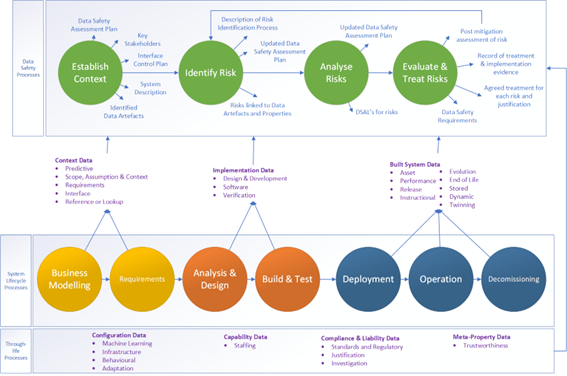
\includegraphics[angle=90]{images/Lifecycle}
\caption{Simplified Process Overview}
\label{fig:process}
\end{figure}
Figure \ref{fig:process} provides an overview of the data safety management process and how it integrates with a typical system lifecycle. Data pervades all aspects of a systems lifecycle, so the data safety assessment process can occur throughout the system lifecycle depending on the type of data that is being assessed. Some data items such as context, implementation and built system data are relevant for specific process phases of the lifecycle, while others such as configuration, capability, compliance and liability data apply throughout the entire lifecycle. The meta-property data of trustworthiness covers data that is used to inform on the overall trustworthiness of the system. The specific data categories are covered in more detail in section \ref{bkm:datacategories}.

The data safety management process occurs over four key steps as shown in the top part of the diagram and the specific objectives and outputs of each step is described in more detail in section \ref{bkm:objectivesoutputs}. The last outcome of the process is a post mitigation risk assessment. If the risk reduction is not considered adequate then the process will iterate again from the `identify risk' step. The whole process is intended to be repeated through the lifecycle of the system and so will be repeated many times and further iterations will be required when there are changes to the system or its data.

The bottom section of the figure shows a typical basic lifecycle for a system from its inception through to decommissioning. The types of data that are of concern for each process step including those that apply to all steps are shown and these feed into the data safety assessment process. Further examples of lifecycles are given in Appendix \ref{bkm:lifecycle}.
\cbend

%\newpage
%\subsection{Summary Figure}
%\begin{figure}[!h]
  %\centering
  %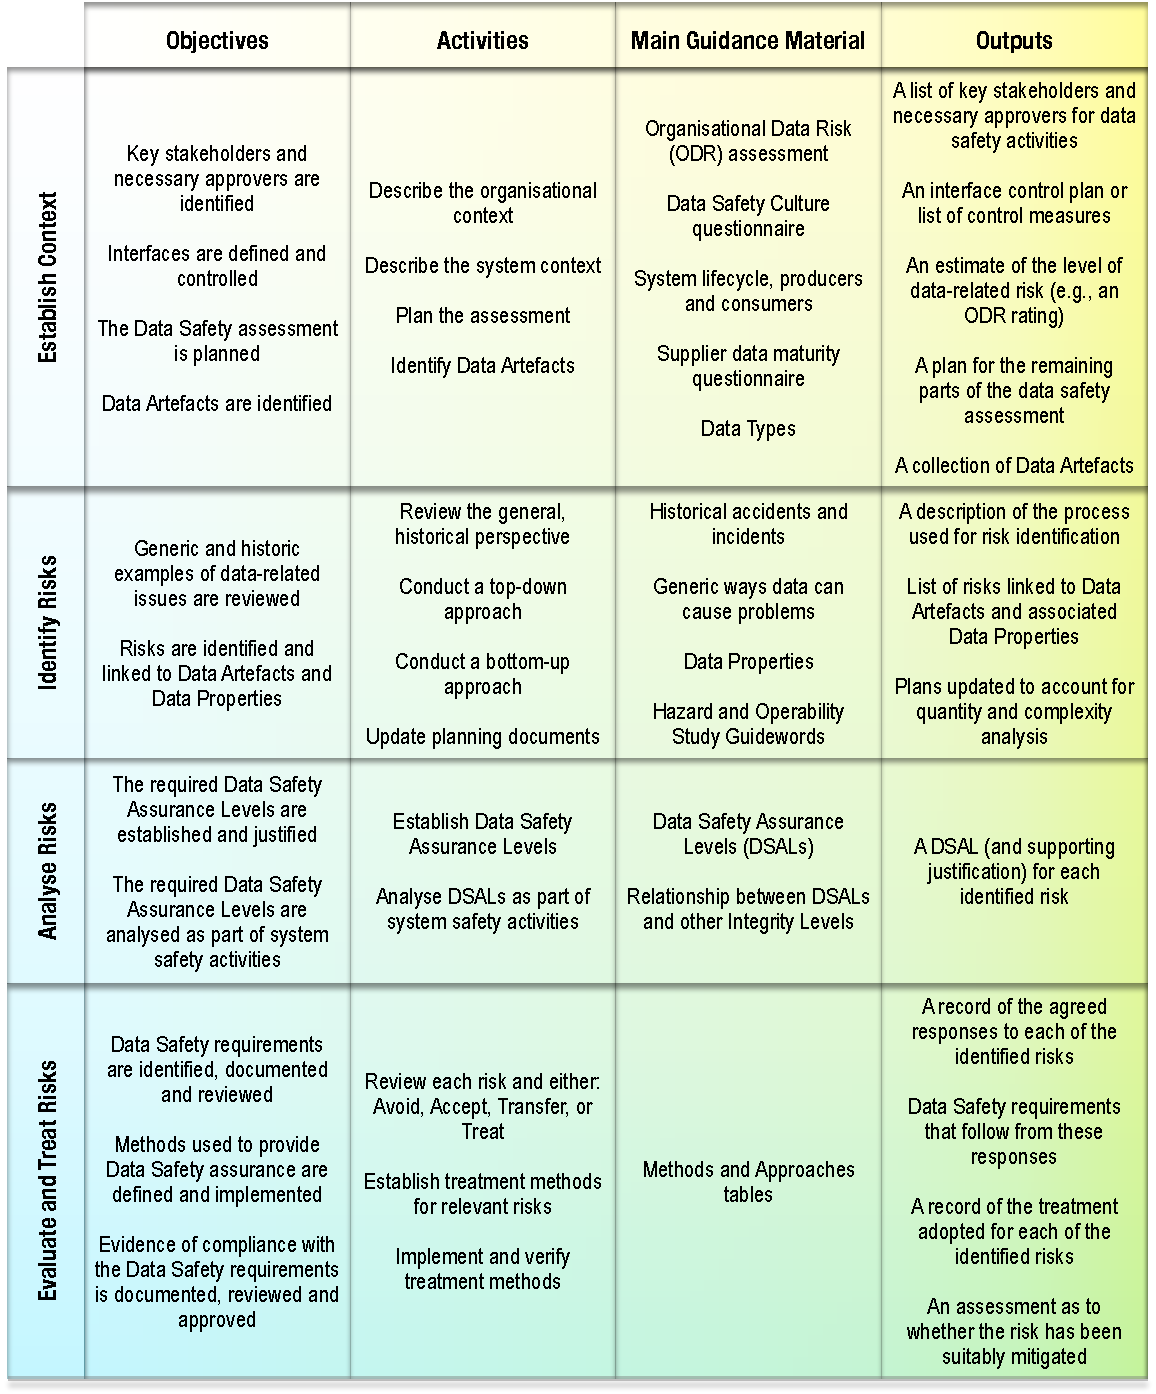
\includegraphics[width=\textwidth]{images/summaryfigure}
  %\label{fig:summaryfigure}
%\end{figure}

%================================================================================
%       Safety Critical Systems Club - Data Safety Initiative Working Group
%================================================================================
%                       DDDD    SSSS  IIIII  W   W   GGGG
%                       D   D  S        I    W   W  G   
%                       D   D   SSS     I    W W W  G  GG
%                       D   D      S    I    WW WW  G   G
%                       DDDD   SSSS   IIIII  W   W   GGG
%================================================================================
%               Data Safety Guidance Document - LaTeX Source File
%================================================================================
%
% Description:
%   Definitions and Abbreviations (Normative) section.
%
%================================================================================
\section{Definitions (Normative)} \label{bkm:definitionsabbreviations}

\dsiwgSectionQuote{I love data. I think it's very important to get it right, and I think it's good to question it.}{Mary Meeker}

\subsection{Definitions}
\begin{longtable}{|L{\dsiwgColumnWidth{0.35}}|L{\dsiwgColumnWidth{0.65}}|}
  \caption{\protect Normative definitions\protect}
  \\\hline\TableHeadColour{Term} & \TableHeadColour{Definition}\\\hline
  \endfirsthead
  \caption[]{Basic definitions (continued)}
  \\\hline\TableHeadColour{Term} & \TableHeadColour{Definition}\\\hline
  \endhead
  \multicolumn{2}{r}{\sl Continued on next page}
  \endfoot
  \endlastfoot
	{Data Artefact\index{Artefact, Data|textbf}} & {An item, or collection of items, that provides a useful perspective on data generated, processed or consumed by a system.}\\\hline
	{\index{Data!Owner|textbf}Data Owner} & {The individual or organization responsible for a particular \index{Artefact, Data}Data Artefact, or collection of Data Artefacts.}\\\hline
	{\index{Property!Data|textbf}\index{Data!Property|see{Property, Data}}Data Property} & {A characteristic that can be exhibited by a \index{Artefact, Data}Data Artefact.}\\\hline
	{\index{Safety Assessment!Data|textbf}\index{Data!Safety Assessment|see{Safety Assessment, Data}}Data Safety Assessment} & {The process of explicitly considering data as part of a \index{Safety Assessment!System}system safety assessment, via the means of \index{Artefact, Data}Data Artefacts, Data Properties and Data Safety Assurance Levels.}\\\hline
	{\index{Data Safety Assurance Level|see{Assurance Level, Safety, Data}}\index{Assurance Level!Safety!Data}Data Safety Assurance Level} & {An indication of the level of rigour with which relevant Data Properties should be demonstrated for appropriate \index{Artefact, Data}Data Artefacts.}\\\hline
	{\index{Safety Requirement!Data|textbf}\index{Data!Safety Requirement|see{Safety Requirement, Data}}Data Safety Requirement} & {A requirement to implement an approach specifically designed to achieve, maintain or demonstrate a Data Property (or Properties) for a given \index{Artefact, Data}Data Artefact (or Artefacts).}\\\hline
    {\index{Response|textbf}Response} & {The way in which an identified risk is addressed; possible responses include avoid/eliminate, treat, or accept as sufficiently low.}\\\hline
	{\index{Stakeholder|textbf}Stakeholder} & {An individual or organization that has some relationship to the system, possibly including a power of veto.}\\\hline
    {\index{Treatment!Risk|textbf}Treatment} & {An action taken to reduce or control risk.}\\\hline
\end{longtable}

A more comprehensive list of definitions, including descriptive definitions, is included at \autoref{bkm:acronyms}.
%-- We don't currently have any normative abbreviations
%\subsection{Abbreviations}
%\textcolor{blue}{XXX TO COMPLETE XXX}

%================================================================================
%       Safety Critical Systems Club - Data Safety Initiative Working Group
%================================================================================
%                       DDDD    SSSS  IIIII  W   W   GGGG
%                       D   D  S        I    W   W  G   
%                       D   D   SSS     I    W W W  G  GG
%                       D   D      S    I    WW WW  G   G
%                       DDDD   SSSS   IIIII  W   W   GGG
%================================================================================
%               Data Safety Guidance Document - LaTeX Source File
%================================================================================
%
% Description:
%   Objectives and Outputs section.
%
%================================================================================
\section{Objectives and Outputs (Normative)} \label{bkm:objectivesoutputs}

\dsiwgSectionQuote{The goal is to turn data into information, and information into insight.}{Carly Fiorina}

\subsection{Establish Context}
\subsubsection{Objectives}
\begin{enumerate}[label=\color{dsiwgAccentColour}{1-\arabic*}]
	\item System context and intended use SHALL be established.
	\item Key \index{Stakeholder}Stakeholders SHALL be identified.
	\item \index{Artefact, Data}Glspl{Data Artefact} SHALL be identified.
	\item Interfaces SHALL be defined and managed.
	\item A \index{Safety Assessment!Data}Data Safety Assessment SHALL be planned.
\end{enumerate}

\subsubsection{Outputs}
\begin{itemize}
	\item A description of the system and its intended use. This SHOULD include an estimate of the level of data-related risks.
	\item A list of key \index{Stakeholder}Stakeholders for data safety activities.
	\item A collection of \index{Artefact, Data}\glspl{Data Artefact}, described at an appropriate level of detail.
	\item An interface control plan or list of control measures. This MAY include a list of \index{Data!Owner}\glspl{Data Owner}, linked to \index{Artefact, Data}\glspl{Data Artefact}.
	\item A plan for the remaining parts of the Data Safety Assessment.
\end{itemize}

\subsection{Identify Risks}
\subsubsection{Objectives}
\begin{enumerate}[label=\color{dsiwgAccentColour}{2-\arabic*}]
	\item Historical data-related accidents and incidents SHALL be reviewed.
	\item Unintended behaviour resulting from data SHALL be identified and analysed.
	\item Risks SHALL be identified and linked to \index{Artefact, Data}\glspl{Data Artefact} and \index{Property!Data}Data Properties.
\end{enumerate}

\subsubsection{Outputs}
\begin{itemize}
	\item A description of the process used for risk identification.
	\item A list of risks, linked to \index{Artefact, Data}\glspl{Data Artefact} and \index{Property!Data}Data Properties.
	\item An updated plan for the remaining parts of the Data \index{Safety Assessment!Data}Safety Assessment, if required.
\end{itemize}

\subsection{Analyse Risks}
\subsubsection{Objectives}
\begin{enumerate}[label=\color{dsiwgAccentColour}{3-\arabic*}]
	\item Data Safety Assurance Levels SHALL be established.
	\item Data Safety Assurance Levels SHALL be justified.
	\item Data Safety Assurance Levels SHALL be incorporated into system safety activities.
\end{enumerate}

\subsubsection{Outputs}
\begin{itemize}
	\item A Data Safety Assurance Level and supporting justification\index{Justification, Safety} for each risk identified in the previous phase.
	\item An updated plan for the remaining parts of the \index{Safety Assessment!Data}Data Safety Assessment, if required.
\end{itemize}

\subsection{Evaluate and Treat Risks}
\subsubsection{Objectives}
\begin{enumerate}[label=\color{dsiwgAccentColour}{4-\arabic*}]
	\item \index{Safety Requirement!Data}Data Safety Requirements SHALL be established and elaborated.
	\item Methods used to provide data safety assurance SHALL be defined and implemented.
	\item Compliance with \index{Safety Requirement!Data}Data Safety Requirements SHALL be demonstrated.	
\end{enumerate}

\subsubsection{Outputs}
\begin{itemize}
	\item A record of the agreed \index{Response}responses to each of the identified risks, along with supporting justification\index{Justification, Safety}.
	\item A list of \index{Safety Requirement!Data}Data Safety Requirements that follow from these \index{Response}responses.
	\item A record of the \index{Treatment!Risk}treatment adopted for each of the identified risks, including evidence that the \index{Treatment!Risk}treatment has been successfully implemented.
	\item An assessment as to whether the risk has been suitably mitigated\index{Mitigation} (and, if not, plans for further mitigation\index{Mitigation} activities).
\end{itemize}

%================================================================================
%       Safety Critical Systems Club - Data Safety Initiative Working Group
%================================================================================
%                       DDDD    SSSS  IIIII  W   W   GGGG
%                       D   D  S        I    W   W  G   
%                       D   D   SSS     I    W W W  G  GG
%                       D   D      S    I    WW WW  G   G
%                       DDDD   SSSS   IIIII  W   W   GGG
%================================================================================
%               Data Safety Guidance Document - LaTeX Source File
%================================================================================
%
% Description:
%   Activities and Tailoring section.
%
%================================================================================
\section{Activities and Tailoring (Informative)} \label{bkm:activitiestailoring}

\dsiwgSectionQuote
  {It is a capital mistake to theorise before one has data.}
  {Sherlock Holmes - ``A Study in Scarlet'' (Sir Arthur Conan Doyle)}


\subsection{Establish Context}
\subsubsection{Overview}
This phase involves developing: an understanding of the context within which the system development occurs; an understanding of the system requirements; and an understanding of the system design.
These factors help determine the risk appetite; that is, essentially, how much effort will be devoted to making risks as low as practicable. In turn, this will inform the nature and scope of assessments that are conducted during system development, introduction to service and operation. The factors also help identify \index{Stakeholder}Stakeholders.

\subsubsection{Activities}
There are four activities associated with this phase.

\paragraph{Describe the organizational context}
Part of this activity involves understanding the \index{Stakeholder}Stakeholders involved, or with an interest, in the system. It is important to define how the \index{Stakeholder}Stakeholders will interact and the derived requirements applicable to each \index{Stakeholder}Stakeholder through interface control\index{Interface!organizational}, similarly to systems engineering interface control procedures already in place in many industries. Consideration of external (e.g., economic, social, regulatory) and internal (e.g., culture, processes, strategy) factors is key to defining appropriate interface control measures. Note that, similarly to requirements, interface control may be iterative throughout the \index{Safety Assessment!Data}Data Safety Assessment. In particular, interface control may need to be amended to take account of implemented data safety mitigations\index{Mitigation}.

To form
a high-level understanding of each organization's risk,
the \gls{odr} assessment (\autoref{bkm:assessment}) can be used. The \gls{odr} assessment can be used at programme level to cover all \index{Stakeholder}Stakeholders, or used by each individual \index{Stakeholder}Stakeholder to determine the
risk
appropriate to their area.
Note however that care should be taken when adopting such a formulaic approach to risk assessment
to ensure that the resulting system can meet its cumulative requirements; that is, nothing has ``fallen through the cracks''. This is part of the requirements decomposition and verification / validation activities described later in the Data Safety Management Process.

Amongst other things, the \gls{odr} assessment includes: the severity of any potential accidents; organizational maturity; applicable legal and regulatory frameworks; and the size, complexity and novelty of the planned system. It results in a rating, from ODR0 (which corresponds to the lowest risk) to ODR4 (which corresponds to the highest risk). This rating provides an initial, top-level view of the magnitude of data-related risk. As such, it
could form
the basis for process tailoring; it also
gives an indication of the proportionate magnitude of effort that may be required in the management of data safety risks.

To allow tailoring to be applied in cases where the \gls{odr} assessment has not been explicitly conducted, the qualitative scale presented in \autoref{tab:Qualitative-ODR} is also used.

\begin{longtable}{|C{\dsiwgColumnWidth{0.21}}|L{\dsiwgColumnWidth{0.39}}|}
  \caption{Qualitative definition of \glsfmtshort{odr}}
  \label{tab:Qualitative-ODR}
  \\\hline\TableHeadColourCX{\glsfmtshort{odr} Rating} & \TableHeadColour{Qualitative Description}\\\hline
  \endfirsthead
  \caption[]{Qualitative definition of \glsfmtshort{odr} (continued)}
  \\\hline\TableHeadColourCX{\glsfmtshort{odr} Rating} & \TableHeadColour{Qualitative Description}\\\hline
  \endhead
  \multicolumn{2}{r}{\sl Continued on next page}
  \endfoot
  \endlastfoot
  {ODR4} & {High risk}\\\hline
  {ODR3} & \multirow{2}*{Medium risk}\\\cline{1-1}
  {ODR2} &\\\hline
  {ODR1} & {Low risk}\\\hline
  {ODR0} & {Very low risk}\\\hline
\end{longtable}

Note that, in the case of an ODR0, no further work is required.

In addition to the rating, the \gls{odr} can be used to facilitate the identification of key \index{Stakeholder}Stakeholders (i.e., those with an interest in the system) and necessary approvers (i.e., those who need to formally accept the system). Note that some approvers might be within the organization, while others may represent external bodies. Likewise, approvers could also be customers or regulatory authorities.

Part of the process of establishing the internal context involves understanding organizational culture. A short Data Safety Culture questionnaire has been developed (\autoref{bkm:culture}), which may help in this regard. This can be applied at an organization level or, more likely, within an individual project team. The questionnaire could also be used to highlight the importance of data safety related issues within a project team. In addition, before and after measurements could be taken to establish the effectiveness of data safety related training.

\paragraph{Describe the system context}
This activity is concerned with describing the system under analysis, as well as the key external influences on that system (examples of which include interfacing systems and human operators). There are obviously many aspects to this activity. For reasons of brevity only those aspects that are directly relevant to data safety are discussed here.

When describing the system it is often helpful to think in terms of producers and consumers of data. These may be external systems, or sub-systems, or a combination of both. In addition, it may be necessary to consider data supply chains, especially when there are a number of separate organizations involved. Note that the considerations discussed in this paragraph are intended to be addressed at a high level: the identification of specific pieces of data is a separate, but related, activity; the identification of required properties is another activity.

Also note that, as development progresses the system description is expected to be refined. This may enable the data safety system context to also be refined, supporting the \index{Safety Assessment!Data}Data Safety Assessment planning.

\paragraph{Plan the assessment}
This activity involves scheduling the phases associated with the Data Safety Management Process and acquiring the necessary resources to complete them. This also involves tailoring the generic process to meet the specific needs of a particular system development. 

Details of the planned assessment may be recorded in a \gls{dsmp}. This could also be used to capture the scope of the analyses and the associated context. Together, this \gls{information} constitutes the first section of the \gls{dsmp} structure. Note that if a \gls{dsmp} is created, it would be expected to be updated with details from subsequent phases. Alternatively, if a Safety Management Plan has already been developed for the project, data safety aspects may augment the existing Safety Management Plan. 

Planning of the \index{Safety Assessment!Data}Data Safety Assessment requires some knowledge of the quantity and complexity of data that requires assessment. Therefore, the \gls{dsmp} (or Safety Management Plan) needs to be updated in subsequent phases once these details are known.

Planning of the assessment may be done through a procurement process. Procurers may wish to understand their potential supplier's understanding of data safety and plans to implement a \index{Safety Assessment!Data}Data Safety Assessment. A Data Safety Supplier Questionnaire (\autoref{bkm:maturity}) has been developed to support this analysis; this questionnaire may also be used for auditing purposes.

\paragraph{Identify \index{Artefact, Data}Data Artefacts}
\index{Artefact, Data}Data Artefacts are the key pieces of data that are generated, processed or consumed by the system, or used for training in its use or maintenance. They provide the foundation for the remaining phases of data-related risk management.

To support the identification of \index{Artefact, Data}Data Artefacts, a wide variety of Data Categories have been enumerated. Cross-referencing these categories against the system description should highlight the relevant artefacts. 

Another way of identifying \index{Artefact, Data}Data Artefacts involves considering the functions that the system performs and establishing the data that is required to support these.

A further option for confirming that all relevant \index{Artefact, Data}Data Artefacts have been identified is to consider the different phases of the system lifecycle\index{Lifecycle!System}. This approach should help prevent an inappropriate focus on operational use of the system at the expense of, for example, artefacts associated with system test and evaluation.

\subsubsection{Tailoring}
The level of
\index{Stakeholder}stakeholder
interface control\index{Interface!organizational} required will depend heavily on the number of \index{Stakeholder}Stakeholders, complexity of their interactions, and the contractual controls already in place. Many programmes already require \glspl{icd}\index{Interface!Control Document} to be developed for systems or equipment. The level of detail required in other programme interface control plans may be used as a guide for the requirements of data safety interface control. 

The guidance in this document is general in nature and so it is anticipated that it will need to be tailored to align with the organization's attitude to risk, their existing processes and the relevant sector's regulatory environment. Thus the provided \gls{odr}, or a version customised to suit the organization's needs, may provide a structured approach to assessment.
The \gls{odr} assessment can be conducted at product line or individual product level, as appropriate for the organization. It is generally not recommended to conduct the \gls{odr} without the context of a system type.

It is expected that the \gls{odr} assessment will be of most utility for organizations that do not have significant safety engineering experience and that are operating in less well-regulated industrial sectors.
organizations with considerable experience in the development of safety-critical systems in heavily regulated environments
may also find it of use in defining the context from a data perspective and augmenting existing safety standards which have no explicit data considerations.
Note that if this assessment is not conducted, some high-level qualitative estimate of risk may still be required (e.g., to support process tailoring); likewise, there will also be a need to identify key \index{Stakeholder}Stakeholders and necessary approvers.

It is also expected that the Data Safety Culture questionnaire will be of most use for low-risk (i.e., ODR1) systems. In particular, it is expected that developers of higher risk systems will have extant processes to develop, maintain and monitor safety cultures,
although the data-oriented questionnaire could help inform those existing processes.

The approach of including data-related aspects within a Safety Management Plan is recommended for complex or highly safety-critical systems. In this case the structure of the Safety Management Plan may be maintained, with the \index{Safety Assessment!Data}Data Safety Assessment process being tailored to align to the overall \index{Safety Assessment}safety assessment process.

The questionnaire that helps establish the level of ``data maturity'' in potential suppliers is expected to be of most use when new organizational relationships are being formed. Conversely, it may offer little value in situations where both organizations are familiar with each other, they have worked on data-related projects together before and there are suitable audit / review arrangements in place.

\index{Artefact, Data}Data Artefacts may be defined at a number of levels. An artefact associated with a medical system could be described as ``patient data''. Alternatively, this could be split into smaller parts (e.g., ``blood group''). Generally speaking, the highest possible level consistent with the system description should be used; this prevents an excessively long list of artefacts being developed. If necessary, those artefacts where further detail is needed can be refined as part of an iterative process that is focused on key issues.

Not every Data Category\index{Data!Category|} will be relevant to every system. Furthermore, for low-risk (ODR1) systems it may be sufficient to simply consider the groupings of categories (e.g., ``context'', ``implementation'', etc.). Conversely, high-risk (ODR4) systems might need to consider every category\index{Category!Data}, even if this results in a conclusion that a specific category\index{Category!Data} is not relevant for the system in question.

A function-based approach to identifying \index{Artefact, Data}Data Artefacts is likely to be enabled by design processes that also adopt a function-based perspective. If \gls{information} from a function-based perspective is readily available then it should be used to support the identification of \index{Artefact, Data}Data Artefacts. If this \gls{information} is not readily available, it is recommended that it be generated for medium and high-risk systems (i.e., ODR2 to ODR4, inclusive).

Considering data across the system lifecycle\index{Lifecycle!System} is a relatively simple activity, which is applicable to all systems (i.e., ODR1 to ODR4, inclusive).

\subsection{Identify Risks}
\subsubsection{Overview}
This phase involves identifying sources of risk and understanding the potential consequences; it should result in a comprehensive list of risks. From a system development perspective, these activities are likely to be concurrent with the development of more detailed system designs.

\subsubsection{Activities}
There are three, complementary, activities that can be used to identify risks. There is also an activity associated with updating planning documents.

\paragraph{Review the general, historical perspective}
Some insight into potential risks may be gained by reviewing historical accidents and incidents, a collection of which is included in
\autoref{bkm:accidents} of this guidance document. It is expected that each domain would have its own catalogue of historical incidents, which can be consulted during a data-focused review.

\paragraph{Conduct a top-down approach}
If the system under consideration has clearly identified functions then data-related risks can be assessed by considering each function in turn and analysing what \index{Artefact, Data}Data Artefacts and, more particularly, what Data Properties the function depends on.

If there are a limited number of safety-related functions, this is usually the simplest approach. This approach also has the advantage that it integrates well with other function-based, top-down approaches to assessing system safety. 

\paragraph{Conduct a bottom-up approach}
This approach starts from the Data Artefacts and explores the effects of \glspl{error}. In this context an error is a situation where a required \index{Property!Data}Data Property is not exhibited. This may be achieved by a variety of methods, including a \gls{hazop}\index{HAZOP}.

\paragraph{Update planning documents}
Once the data safety risks have been identified, the \gls{dsmp} (or Safety Management Plan)
requires review to determine if it needs
updating to take account of the quantity and complexity of the analysis and mitigation\index{Mitigation} activities needed to address the risks. While the \gls{dsmp} may be updated throughout the \index{Safety Assessment!Data}Data Safety Assessment, updates may not be required for all projects.

\subsubsection{Tailoring}
The general, historical perspective review is a simple activity that does not require significant resources. Hence, it is recommended for all systems, regardless of risk level.

When conducting a bottom-up approach, it may not be appropriate to explicitly consider every possible property for every single artefact. In particular, for low-risk (ODR1) and medium-risk (ODR2 / ODR3) systems some form of tailoring may be expected: this may, for example, take the form of pre-selecting the properties that are most relevant, or limiting the layer of abstraction at which the system is considered.

Tailoring of the bottom-up approach may also be appropriate for some high-risk (ODR4) systems, but in this case an explicit argument that the tailoring has not adversely affected system safety would be expected. Furthermore, the risk identification process for high-risk (ODR4) systems is expected to be a highly structured affair. To support this, a number of data-related \gls{hazop}\index{HAZOP} Guidewords have been determined
and are presented in \autoref{bkm:guidewords}.

The top-down and bottom-up approaches provide different perspectives when attempting to identify data-related risks. For low-risk (ODR1) systems it may be appropriate to consider just one of these perspectives. Conversely, both perspectives would be expected to be considered (to some degree) for medium-risk (ODR2 / ODR3) and high-risk (ODR4) systems.
%
%\clearpage %Manual page break
\subsection{Analyse Risks}
\subsubsection{Overview}
This part of the risk management process involves developing an understanding of the consequences and likelihood of each risk. From the perspective of safety-critical and safety-related systems this understanding allows system (or safety) \gls{integrity} levels or \index{Assurance Level!Development}Development Assurance Levels to be determined. Likewise, this understanding should be used to allocate
\glspl{dsal}\index{Assurance Level!Data}\index{DSAL|see{Assurance Level, Data}}.
%
%\vspace{-8pt}%Cheat needed to avoid table bleeding over to next page. Only needed since file indexed!
%
\subsubsection{Activities}
There are two activities associated with this phase.
%
\paragraph{Establish \glsfmtshort{dsal}}\index{Assurance Level!Data|textbf}
\label{bkm:DSAL-table-section}
The key activity in this phase is to establish the (untreated) likelihood and severity of each risk identified in the preceding phase.

To analyse risks and, more particularly, to align data safety with other risk management processes, there is a need to overcome problems stemming from the use of the term ``likelihood'' in situations where there may be no failure rates. For this reason the \gls{dsal}\index{Assurance Level!Data} was developed. The \gls{dsal} metric is not a statistical measure of likelihood, or a literal numeric measure of \index{Integrity Property}\gls{integrity}. Instead, the \gls{dsal} metric is an indicator for the level of rigour that an assurance argument requires. As such, \glspl{dsal} share a common theoretical basis with concepts like \glspl{idal} \index{Assurance Level!Development} \cite{citation:arp4754a2010guidelines} and development process systematic capability \cite{citation:iec615083}.

\glspl{dsal} are measured on a scale of DSAL0 (lowest-assurance) to DSAL4 (highest-assurance). They are typically allocated as indicated in \autoref{tab:DSAL-risk-matrix}.

\begin{longtable}{|C{\dsiwgColumnWidth{0.2}}|C{\dsiwgColumnWidth{0.2}}|C{\dsiwgColumnWidth{0.2}}|C{\dsiwgColumnWidth{0.2}}|}
  \caption{\glsfmtshort{dsal} ``Risk'' Matrix}
  \label{tab:DSAL-risk-matrix}
  \\\hline
  \TableHeadColour{} & \multicolumn{3}{c|}{\TableHeadColourCX{Likelihood}}\\\cline{2-4}
  \multirow{-2}*{\TableHeadColourCX{Severity}} & \TableDimColourCX{ High} & \TableDimColourCX{Medium} & \TableDimColourCX{Low}\\\hline
  \endfirsthead
  \caption[]{\glsfmtshort{dsal} ``Risk'' Matrix (continued)}
  \\\hline
  \TableHeadColour{} & \multicolumn{3}{c|}{\TableHeadColourCX{Likelihood}}\\\cline{2-4}
  \multirow{-2}*{\TableHeadColourCX{Severity}} & \TableDimColourCX{High} & \TableDimColourCX{Medium} & \TableDimColourCX{Low}\\\hline
  \endhead
  \multicolumn{4}{r}{\sl Continued on next page}
  \endfoot
  \endlastfoot
  Minor & DSAL1 & DSAL0 & DSAL0\index{Assurance Level!Data}\\\hline
  Moderate & DSAL2 & DSAL1 & DSAL0\index{Assurance Level!Data}\\\hline
  Significant & DSAL3 & DSAL2 & DSAL1\index{Assurance Level!Data}\\\hline
  Major & DSAL4 & DSAL3 & DSAL2\index{Assurance Level!Data}\\\hline
  Catastrophic & DSAL4 & DSAL4 & DSAL3\index{Assurance Level!Data}\\\hline
\end{longtable}

Definitions for Severity and Likelihood associated with \autoref{tab:DSAL-risk-matrix} may be customised for a specific application. A default approach to the assessment of Likelihood is presented in
\hyperref[bkm:Establishing-DSALS]{section}\index{Assurance Level!Data}~\ref{bkm:Establishing-DSALS} %Clunky, but \autoref inserted "subsubsection"
and \autoref{tab:Likelihood}, while default definitions for Severity are presented in \autoref{tab:Severity}.

Although this allocation of \glspl{dsal}\index{Assurance Level!Data} is typically used, it is acknowledged that there are some situations where a different allocation matrix may be more appropriate. Hence, it may be appropriate for a tailored allocation matrix to be used. Regardless of whether tailoring is used, the matrix should be reviewed and confirmed as being suitable for the intended application.

As their name suggests, \glspl{dsal} are focused on safety concerns. However, the framework of \index{Artefact, Data}Data Artefacts, \index{Property!Data}Data Properties, and so on, developed in this document could also be applied to other concerns. It could, for example, be used for to control data-related financial risks, or data-related reputational risks. In these types of approach, the severity terms would obviously relate to financial and reputational consequences, rather than safety ones.

It is possible that the additional understanding developed during this part of the process may mean some previously identified Data Artefacts are no longer of consequence; similarly, it is possible that this process may identify additional artefacts or a need to refine the description of existing artefacts.

\paragraph{Analyse \glspl{dsal} as part of system safety activities}\index{Assurance Level!Data}
\label{bkm:activities:analyse:partofsystemsafetyactivities}
Allocating a \gls{dsal}\index{Assurance Level!Data} is a significant part of controlling data safety risks, but it is not the only part. It is important that \glspl{dsal} are considered as part of wider system safety activities, rather than being viewed as a separate item.

For medium-risk (ODR2 / ODR3) and high-risk (ODR4) systems it is likely that \index{Integrity Property}\gls{integrity}, or assurance, levels will be calculated from perspectives other than data safety. Possible examples include Item / Function \index{Assurance Level!Development}Development Assurance Levels from \glspl{arp} 4754A \cite{citation:arp4754a2010guidelines} and safety \gls{integrity} levels from IEC 61508 \cite{citation:iec615083}.
Where such an approach is used, the mapping to \glspl{dsal}\index{Assurance Level!Data} should be included within the \gls{dsmp}.

This activity involves comparing \glspl{dsal}\index{Assurance Level!Data} with these other \gls{integrity}, or assurance, levels. Assuming a typical scenario of a system processing or manipulating data flowing through it, there are two cases to consider:

\begin{enumerate}
  \item Can the data affect the software? In particular, this question is concerned with whether the data can affect the software such that the safe operation of the system is jeopardised. Obviously an ideal system would be able to handle any data fed into it safely without problems, but this is often not the case. An example might be a legacy system which has limited error checking and so may fail in unsafe ways if fed with data which is outside of the expected range. Formally this question can be stated as: \dsiwgTextIT{Given a system containing software written to a particular \index{Assurance Level!Software}\cbstart\gls{software assurance level}\cbend\ (which may be none), what should the \gls{dsal}\index{Assurance Level!Data} of the processed data be to preserve correct operation of the system?}
  \item Can the software affect the data? In particular, this question is concerned with whether the system's software can affect the data being processed or manipulated in such a way that \index{Property!Data}Data Properties that are important for safety might be lost. Some examples might be systems which transform messages, losing any associated checksum protections, thereby possibly affecting the \index{Integrity Property}\gls{integrity} of the data within the message; as a minimum, this removes a means of checking data \index{Integrity Property}\gls{integrity}. Another example might be a system that can delay data flowing through it, (e.g., due to buffering) when timely delivery of the data is critical. Formally, this question can be stated as: \dsiwgTextIT{Given data at a particular \gls{dsal}\index{Assurance Level!Data} what should the \index{Assurance Level!Software}\gls{software assurance level} of the software in the system be in order to preserve the \gls{dsal}\index{Assurance Level!Data} of the data?}
\end{enumerate}

\subsubsection{Tailoring}\label{bkm:activities:analyse:tailoring}
\glspl{dsal}\index{Assurance Level!Data} can be applied at different levels and to different constructs. For example, in the case of simple, low-risk systems it may be appropriate to apply a single \gls{dsal} to an entire system. Alternatively, it may be appropriate to apply \glspl{dsal} to sub-systems, for example, to match the level at which other \gls{integrity}, or assurance, levels have been determined. 

Another option is to apply \glspl{dsal}\index{Assurance Level!Data} to Data Artefacts rather than directly to risks. This approach has the advantage that \index{Treatment!Risk}treatments are often related to artefacts; it can work well where there is a simple relationship between artefacts and risks.

%\clearpage %Manual page break
\subsection{Evaluate and Treat Risks}
\subsubsection{Overview}
This phase involves deciding, at a generic level, what action (if any) should be taken for each of the risks identified in preceding phases. This decision will be influenced by the organization's risk appetite and other factors determined as part of the Establish Context phase. From some perspectives it may seem strange that requirements are identified at such a late phase. This is a consequence of explicitly linking \index{Safety Requirement!Data}Data Safety Requirements to risks associated with \index{Property!Data}Data Properties of \index{Artefact, Data}Data Artefacts, and the use of \index{Assurance Level!Data}\glspl{dsal} to describe levels of rigour. 

This phase also involves identifying, implementing and verifying \index{Treatment!Risk}treatments for the risks emerging from the previous phase. Part of verifying the \index{Treatment!Risk}treatment involves checking technical details of the chosen approach; another part involves re-assessing the post-treatment risk to determine whether it is now acceptable.

\subsubsection{Activities}
This phase involves reviewing each risk, including the associated \gls{dsal}\index{Assurance Level!Data} and determining the appropriate \index{Response}response. Essentially, this phase aims to answer the question: can we accept this risk or does some action need to be taken? This is likely to require discussion amongst a number of \index{Stakeholder}Stakeholders. From a system safety perspective, there is nothing intrinsically special about data-related risks. Hence, it is recommended that evaluation of data-related risks be conducted alongside the evaluation of other system risks, as part of an organization's standard risk evaluation process.

Risks may be managed in different ways, for example:

\begin{itemize}
  \item \nonumparagraph{Avoid}
	
	Risk avoidance can be employed where a risk can be eliminated by using different approaches to the design and / or operation of the system. It may also be the case that very significant risks cannot be adequately treated and the only option is to avoid the untenable risk by not proceeding with the project.

  \item \nonumparagraph{Accept} 
	
    For low likelihood and low severity risks (e.g., those ranked as DSAL0)\index{Assurance Level!Data}, where the cost of further risk reduction is judged to be unacceptable, the risk may be accepted as-is and managed as such. Appropriate justification\index{Justification, Safety} is likely to be required for acceptance of risks ranked higher than DSAL0\index{Assurance Level!Data}.
\clearpage   
  \item \nonumparagraph{Transfer} 
	
	In this case ownership of the risk's consequence is transferred to another organization. This can be achieved, for example, by taking out an insurance policy. It is important that any such risk transfers are formally documented, understood and
	agreed
	by both parties.

  \item \nonumparagraph{Treat} 
	
	In this case there is a desire to reduce the risk. This can be achieved by reducing the severity, or the likelihood or both. Choosing this \index{Response}response often involves having an outline view of how the risk may be reduced. 
\end{itemize}

In addition to deciding on and documenting the appropriate \index{Response}response to each risk, this phase also includes gaining approval for these decisions.

In cases when a decision is made to treat a risk, suitable methods and approaches should be identified. To assist in this process, a range of potential methods and approaches are included in this guidance. These are mapped against \glspl{dsal}\index{Assurance Level!Data}, \index{Property!Data}Data Properties and a selection of lifecycle\index{Lifecycle!Data} data categories.

Once a \index{Treatment!Risk}treatment strategy has been established and implemented there is, of course, a need to determine whether the expected risk reduction has been achieved. Equivalently, there is a need to consider whether the residual risk may now be accepted (or whether another one of the \index{Response}responses identified above is necessary).

\subsubsection{Tailoring}
It is expected that records will be kept of the discussions that occur as part of risk evaluation. For low-risk (ODR1) systems, this may be in the form of a brief memo. Conversely, for high-risk (ODR4) systems, a detailed, structured record, which is placed under formal control, may be expected; in this case these discussions may be recorded as part of the system's \gls{hazard log} or as part of a Data Safety Management Plan.

As outlined in
\hyperref[bkm:activities:analyse:tailoring]{section}~\ref{bkm:activities:analyse:tailoring}, %Clunky, but \autoref inserted "subsubsection"
\glspl{dsal}\index{Assurance Level!Data} can be applied at varying levels of abstraction. For small-scale or low-risk (ODR1) systems it may be appropriate to consider \index{Treatment!Risk}treatments at higher levels of system abstraction. For example, this could involve applying a single \gls{dsal} to a sub-system or even to the system in its entirety and implementing risk \index{Treatment!Risk}treatment techniques at that level. The latter approach could be appropriate where the data in the system interacts in complex ways and the associated safety risk does not warrant a detailed investigation of these interactions.

A significant amount of tailoring is implicit in the way the tables of methods and approaches are constructed. At best a method / approach may be Highly Recommended as a way of maintaining a required \index{Property!Data}Data Property at a given \gls{dsal}\index{Assurance Level!Data}. In addition, the tables are not exhaustive; additional, or alternative, methods and approaches can be used.

%================================================================================
%       Safety Critical Systems Club - Data Safety Initiative Working Group
%================================================================================
%                       DDDD    SSSS  IIIII  W   W   GGGG
%                       D   D  S        I    W   W  G   
%                       D   D   SSS     I    W W W  G  GG
%                       D   D      S    I    WW WW  G   G
%                       DDDD   SSSS   IIIII  W   W   GGG
%================================================================================
%               Data Safety Guidance Document - LaTeX Source File
%================================================================================
%
% Description:
%   Guidance section.
%
%================================================================================
\section{Guidance (Informative)} \label{bkm:guidance}

\dsiwgSectionQuote{I wanted to separate data from programs, because data and instructions are very different.}{Ken Thompson}


\subsection{Establish Context}
\subsubsection{Interface control}\index{Interface!Organizational}
The interfaces between \index{Data!Owner}Data Owners, and indeed data ownership itself, can be much more complicated than for hardware or software, where the owner can be clearly identified. Indeed, when combining items from various sources it is possible to create data for which there is not an ``owner'' in any traditional sense. In such circumstances it may be appropriate for the overall system owner to take responsibility for the collected data and, where appropriate, pass specific, formally-recorded requirements onto original data suppliers. 

The \index{Data!Owner}Data Owners throughout the lifecycle\index{Lifecycle!Data} of data within the system should be identified, or the lack of an owner highlighted where applicable, including where data is merged or modified through the system operation. This will facilitate a greater understanding of the ``controllability'' of data safety issues within the assessment at a particular organizational level.

\subsubsection{Organizational Data Risk Assessment Form}
The \gls{odr} Assessment Form was generated to capture a high-level perspective on the risk posed to an organization by data safety issues within a specific project. How it integrates with an organization's existing risk (or safety) management processes is the responsibility of the implementing organization.
However, it is anticipated that the form could be used to facilitate tailoring of the data safety guidance process.
To facilitate this integration, the following paragraphs describe the connections between the \gls{odr} and the
\acrshort{iso} 31000 \cite{citation:iso310002018risk}
standard for risk management.
The \gls{odr} itself is presented in \autoref{bkm:assessment}.

Establishing the context of a risk assessment ensures that the system being considered and the scope of any assessment is well defined. This helps prevent an overrun of the assessment's boundaries and allows those items that are out of scope to be explicitly communicated to all \index{Stakeholder}Stakeholders. In addition, it is the role of this activity to produce the criteria that a system will be judged on. The \gls{odr} assessment links directly to the sub-tasks identified by \acrshort{iso} 31000 for establishing the risk assessment context and introduces aspects to guide the assessor into focusing on data-specific risks.

Questions 2, 3 and 4 of the \gls{odr} align directly with establishing the external context of the risk assessment
(Activity 6.3.3 from \acrshort{iso} 31000).
They guide the assessor into judging the risk appetite of external \index{Stakeholder}Stakeholders, the level of risk that is allocated to the organization and the regulatory environment within the project will operate.

Question 5 is concerned with establishing the internal context of the risk assessment
(Activity 6.3.3),
inviting the assessor to comment on the maturity of the organization in terms of their attitude not just to risk, but specifically to data-driven risks.

Question 6 explores \index{Data!Owner}data ownership through the use cases of the system. This is related to the legal frameworks explored in Question 4, but also acts to lay the foundations of Activity
6.3.4,
``Defining Risk Criteria'', which requires an assessor to identify ``the nature and types of causes and consequences that can occur and how they will be measured''. This is expanded upon by Questions 1, 7 and 8 which go into data-driven specifics about failure consequences and the issues raised by data complexity, boundary complexity and system complexity for the project.

Finally, the scoring system of the \gls{odr} provides a heuristic for defining the risk criteria
(Activity 6.3.4)
which handles how to combine these different aspects of risk into a single, high-level estimate of the data-related risks associated with a given project. This means that the \gls{odr} can, for example, provide some guidance on Data Safety Assurance Principle ``4 + 1''; that is, it provides some guidance on the amount of effort that should be directed towards the management of data safety issues.
 
It is of note that while the completion of an \gls{odr} fits within the context establishment activity it also augments the ongoing ``communication and consultation'' activity both by providing a standardised format for capturing the relevant information and securing endorsement.

\subsubsection{Data Safety Culture Questionnaire}
Part of the \gls{odr} assessment relates to assessing the organization's maturity in managing data safety risks; \index{Response}responses are aimed at establishing the depth of awareness of data safety and the associated management processes within the organization. However, measuring the level of awareness of processes and concepts in an organization is not always easy. There may be sufficient high-level knowledge of this for the purposes of the \gls{odr} but it still may be an area that warrants further investigation.

To support this, a separate questionnaire has been developed to explore the specific area of measuring the data safety culture for a particular activity; whether this be for the organization as a whole or for a particular project, service or activity. However, here the focus is on a personal view rather than a project or company view so the questionnaire would be completed by all, or a significant subset of, staff. \index{Response}Responses can be aggregated to give an overall data safety culture value. A key aspect of this approach is that it can be periodically repeated to determine trends: for example, if overall scores are declining, this may suggest that further training and briefings will be required.

More details on the Data Safety Culture Questionnaire are provided in \autoref{bkm:culture}.

\subsubsection{System Definition}
The system under consideration should be understood and documented, including interfaces\index{Interface!System} and safety-related data aspects. The process of documenting the system of interest furthers the understanding of \index{Stakeholder}Stakeholders and approvers so they can make sensible judgements about the system. It also formally declares assumptions that are being made while assessing the system and clearly defines the limits of the assessment. In addition, different levels of risk may be associated with composites of safety-related data, which may be easier to manage than individual \index{Artefact, Data}artefacts, or where independence cannot be demonstrated or maintained. Hence, the partitioning of data sets should also be considered during this phase.

\subsubsection{Supplier Data Maturity}
As noted above, a number of usage scenarios involve data being supplied by subcontracted organizations. It is expected that some formal process will be used to select these suppliers. A questionnaire has been developed to help ensure that the supplier has suitable processes in place to manage data safety-related issues. This is available in \autoref{bkm:maturity}.

\subsubsection{Data Categories\index{Category!Data|textbf}}
\label{bkm:datacategories}
The full set of Data Categories which can have safety implications is large: to date more than twenty categories (and one meta-category) have been identified. 

The table below gives the current view of the categories of safety-related data that contribute to, are used by, produced by or affected by safety-related systems. They are roughly organized into a number of categories\index{Category!Data}, which aim to cover all aspects of the system lifecycle\index{Lifecycle!System}. Note that the list in \autoref{tab:CategoriesShort} is non-exhaustive. Also note that a more detailed version of this table is available at \autoref{bkm:categories},
where further detail on each entry is provided.

\begin{longtable}{|C{\dsiwgColumnWidth{0.1}}|L{\dsiwgColumnWidth{0.2}}|L{\dsiwgColumnWidth{0.7}}|}
  \caption{Categories\index{Category!Data} of safety-related data: concise definitions}
  \label{tab:CategoriesShort}
  \\\hline\TableHeadColourCX{No.} & \TableHeadColour{Category} & \TableHeadColour{Description}\\\hline
  \endfirsthead
  \caption[]{Category of safety-related data: concise definitions (continued)}
  \\\hline\TableHeadColourCX{No.} & \TableHeadColour{Category} & \TableHeadColour{Description}\\\hline
  \endhead
  \multicolumn{3}{r}{\sl Continued on next page}
  \endfoot
  \endlastfoot
  \multicolumn{3}{|c|}{\dsiwgTextBF{Context}}\\\hline
  {1} & {Predictive}\index{Predictive Data} & {Data used to model or predict behaviours and performance}\\\hline
  {2} & {Scope, Assumption and Context}\index{Scope, Assumption and Context Data} & {Data used to frame the development, operations or provide context}\\\hline
  {3} & {Requirements}\index{Requirement Data} & {Data used to specify what the system has to do}\\\hline
  {4} & {Interface}\index{Interface Data} & {Data used to enable interfaces between this system and other systems:  for operations, initialisation or export from the system}\\\hline
  {5} & {Reference or Lookup}\index{Reference or Lookup Data} & {Data used across multiple systems with generic usage}\\\hline
  \multicolumn{3}{|c|}{\dsiwgTextBF{Implementation}}\\\hline
  {6} & {Design and Development}\index{Design and Development Data} & {Data produced during development  and implementation}\\\hline
  {7} & {Software}\index{Software Data} & {Data that is compiled (or interpreted) and executed to achieve the desired system behaviour}\\\hline
  {8} & {Verification}\index{Verification Data} & {Data used to test and analyse the system,
    specifically to determine whether it has been built as intended}\\\hline
  \multicolumn{3}{|c|}{\dsiwgTextBF{Configuration}}\\\hline
	{9} & {Machine Learning}\index{Machine Learning Data} & {Data used to train the system}\\\hline
  {10} & {Infrastructure}\index{Infrastructure Data} & {Data used to configure, tailor or instantiate the system itself}\\\hline
  {11} & {Behavioural}\index{Behavioural Data} & {Data used to change the functionality of the system}\\\hline
  {12} & {Adaptation}\index{Adaptation Data} & {Data used to configure to a particular site}\\\hline
  \multicolumn{3}{|c|}{\dsiwgTextBF{Capability}}\\\hline
  {13} & {Staffing}\index{Staffing Data} & {Data related to staff training, competency, certification and permits}\\\hline
  \multicolumn{3}{|c|}{\dsiwgTextBF{The Built System}}\\\hline
  {14} & {Asset}\index{Asset Data} & {Data about the installed or deployed system and its parts, including maintenance data}\\\hline
  {15} & {Performance}\index{Performance Data} & {Data collected or produced about the system during trials, pre-operational phases and live operations}\\\hline
  {16} & {Release}\index{Release Data} & {Data used to ensure safe operations per release instance}\\\hline
  {17} & {Instructional}\index{Instructional Data} & {Data used to warn, train or instruct users about the system}\\\hline
  {18} & {Evolution}\index{Evolution!Data} & {Data about changes after deployment}\\\hline
  {19} & {End of Life}\index{End of Life Data} & {Data about how to stop, remove, replace or dispose of the system}\\\hline
  {20} & {Stored}\index{Stored Data} & {Data stored by the system during operations}\\\hline
  {21} & {Dynamic}\index{Dynamic Data} & {Data manipulated and processed by the system during operations}\\\hline
  {22} & {Twinning}\index{Twinning Data} & {Data used to create and maintain a digital counterpart of a physical object or process}\\\hline
%
  \multicolumn{3}{|c|}{\dsiwgTextBF{Compliance and Liability}}\\\hline
  {23} & {Standards and Regulatory}\index{Standards and Regulatory Data} & {Data that governs the approaches,  processes and procedures used to develop safety systems}\\\hline
  {24} & {Justification} & {Data used to justify the safety position of the system}\\\hline
  {25} & {Investigation}\index{Investigation Data} & {Data used to support accident or incident investigations (i.e., potential evidence)}\\\hline
  \multicolumn{3}{|c|}{\dsiwgTextBF{Meta-Property}}\\\hline
  {+1} & {Trustworthiness}\index{Trustworthiness Data} & {(Meta) data which tells us how much the system can be trusted}\\\hline
\end{longtable}

\subsection{Identify Risks}
\subsubsection{Historical Accidents and Incidents}
Ideally, data safety risks would be identified and mitigated before they led to an accident or incident. However, this is not always the case. Historical occurrences can provide an indication of the data safety risks present in planned or existing systems. In particular, accidents and incidents can be analysed to identify potential contributory causes relating to data.

To support this type of analysis a number of previous accidents and incidents have been collected in \autoref{bkm:accidents}.
These include cases which relate to a number of Data Properties (see
\hyperref[bkm:guidance:dataproperties]{section}~\ref{bkm:guidance:dataproperties}), %Clunky, but \autoref inserted "subsubsection"
for example the properties of \index{Completeness!Property}completeness, \index{Integrity Property}integrity and timeliness\index{Timeliness Property}.
They also highlight the importance of the adaptation Data\index{Adaptation Data} Category\index{Category!Data} and dangers associated with the inappropriate use of default data values.

Most of the current collection of accidents and incidents fall into three categories: aviation; maritime; and medical. However, the lessons that can be learned span a much wider range of application areas.

\subsubsection{Ways that Data Can Cause Problems}
\label{tab:issues}
There are some risk-inducing issues that are different or more prevalent for data than for other system elements. An incomplete collection of examples is provided below. This list may provide a quick way of identifying risks, which could be especially useful at an early stage of a project:

\begin{itemize}
  \item \dsiwgTextBF{Fluidity} Hardware and software can undergo significant amounts of product assurance and once assured may change relatively infrequently. Where change is required to hardware or software, it can be carefully managed and the impact on the safety case appraised. This is not always the case for data, which is often much more fluid; indeed the ease with which data can be changed is one motivation for the move towards data-driven systems. This fluidity means that it is not always possible to revisit safety cases when data changes --- for example, the safety case for an autonomous vehicle cannot be updated every time that the vehicle acquires new knowledge during operation. Instead, the fact that data can change, along with any associated safety impacts, may need to be captured in the system safety case. Fluidity can also provide a temptation for unscrupulous operators to falsify data, for example, after an incident has occurred. Rigorous configuration control procedures can help protect against this type of behaviour.

  \item \dsiwgTextBF{Reuse} For the purposes of this discussion, ``reuse'' is interpreted as use of the same data in a different system or system context (e.g., lifecycle\index{Lifecycle!System} phase). Just because data was valid for use in a particular system, it does not immediately follow that it can be reused again in a similar system. Many considerations associated with data reuse are similar to those of software reuse, for example: similarity of requirements; similarity of role in system; and similarity in required \index{Integrity Property}integrity / \index{Assurance Level}assurance level. One consideration that is different is that of timeliness\index{Timeliness Property}: data that was valid for use in a particular system at a particular time is not necessarily valid for reuse in the same system at a different time.

  \item \dsiwgTextBF{Ageing} As highlighted above, all safety-related data has a lifetime and this needs to be explicitly managed. This can involve, for example, purging, deletion and alerting. It is also important to note that ageing can occur as a result of changes external to the system (for example, records of the positions of other aircraft, newly discovered drug interactions, or new software patches) or it can result from internal changes (e.g., valves gradually becoming less responsive, configuration data becoming out of date, or data schemas evolving over time).

  \item \dsiwgTextBF{Transformation} Data is often filtered, mapped or aggregated as it moves through systems, sometimes creating new data sets as a result. Data Properties are not necessarily preserved by these processes --- sometimes data is filtered too much or only some of the data is selected (either deliberately or inadvertently through accident or unintended bias), such as by the selection of only the test runs that succeeded. The main issues are loss of heritage / history / source information; data can also appear to become something else. Without careful management the \index{Integrity Property}integrity may become lowered to the lowest common denominator and this needs to be recognized. Additional checks (e.g., validation checks, sanity checks) or assurance measures may need to be put in place to ensure that required \index{Integrity Property}integrity / assurance is maintained.

  \item \dsiwgTextBF{\index{Data!Owner}Ownership} The transformation of data can result in a lack of clarity regarding who has ownership of, and responsibility for, the data (if anyone). It is important that responsibility for errors can be tracked, for example, to determine whether they were present in the initial data or whether they arose as part of the transformation process. Establishing clear roles within the data supply chain can help mitigate these issues.

  \item \dsiwgTextBF{Archiving and Retrieval} Safety-related data needs to be available when required. There is thus a need to think about data accessibility over the complete system lifetime. It is also important to consider what \index{Property!Data}properties of the data need to be preserved and how this affects the choice of storage medium.

  \item \dsiwgTextBF{Biasing} This is a systemic \index{Accuracy Property}inaccuracy in data due to the characteristics of the process employed in the creation, collection, manipulation, presentation and interpretation of data. It is usually an unintentional distortion in the data set --- one example of this is the confirmation bias that may be applied to safety claims,
    while another example is that synthetic autonomous vehicle training databases can have issues with artificial data if not realistic.
    Although there is no perfect way of checking for this within the system, \index{Completeness!Checks}completeness, statistical and validity checks on data sets may help.

  \item \dsiwgTextBF{Falsification / Misinformation} This issue arises where data is created, modified or deleted either accidentally or deliberately so as to mislead or misinform potential consumers of that data. Examples from policing and criminal justice might be: notes taken with fabricated times or dates; or accidentally adding or removing a crime from the wrong individual in a database. Another example might be a supplier falsifying quality records for materials or goods. There have been many cases of misinformation related to the Covid-19\index{Covid-19} pandemic (for example on social media) where people have been deliberately misled and sometimes this has led to harm (drinking bleach as a cure for instance). Some mitigations\index{Mitigation} involve digitally signing transmitted data, strong access controls, independent fact-checking and audit records.

  \item \dsiwgTextBF{Defaulting} Many systems use default or initial values for data items; sometimes in data sets and sometimes embedded in software. Often these default values are designed to be neutral (e.g., ``0'') or unrealistic (e.g., ``VOID''). There are essentially two cases: (i) initialisation data which may persist and be mistakenly taken as a real value when in fact it should have been changed; (ii) data that is used when no meaningful value has been assigned (e.g., during data migration or data exchange between systems). These issues can often be managed through good design of data structures, for example by the inclusion of a validity flag.

  \item \dsiwgTextBF{Sentinels} A sentinel value is a data value that is used to indicate a special action needs to be taken, typically indicating the end of a record or a data set. The sentinel value should be one that is not allowable in the data set itself, but often is not properly considered and may use common sequences (e.g., five zeroes). Sentinels can cause problems in two ways: (i) where they are not recognized and so, for example, processing continues past the sentinel; (ii) where the data itself somehow contains the sentinel value and so processing is erroneously interrupted. Sentinels can be a particular risk in long-lived systems and data sets. As with the issue above, the management or elimination of this issue may often be achieved through improved data structures.

  \item \dsiwgTextBF{Aliasing} This is an effect that causes different data to become indistinguishable when accessed; that is, there is only one record when there should be several --- for example, two patients with similar names inadvertently sharing a single set of medical records. This could be due to the way the data is filtered, sampled, indexed, stored or retrieved. The data issues are typically related to loss of resolution\index{Resolution Property} leading to similar data points appearing to be identical. Hence, methods to maintain resolution\index{Resolution Property}, including use of unique indexes, may be beneficial.

    One specific case of aliasing has come to light recently regarding ``Homophones'' --- words which sound the same but are different such as ``Flower'' / ``Flour'' and ``Bare'' / ``Bear'' \cite{citation:homonym}.
    If these words are read out over a phone there may be confusion as to which is intended.
    Location services based on a number of words such as W3W don't avoid all homophones,
    and so there may be issues when the words are given verbally in an emergency. The issue is discussed further in \autoref{bkm:incacc:w3w}.

  \item \dsiwgTextBF{Disassociation} This effect is, in some senses, the opposite of aliasing; there are several records when there should only be one. This could occur, for example, if two records are created for the same individual using slightly different names. It could also arise if different systems use different indexing methods and the association between the indexes becomes corrupted. Again, methods to maintain data resolution\index{Resolution Property} can be beneficial.

  \item \dsiwgTextBF{Masking} This issue can arise if a notable proportion of a data set is of a poor quality, for example, if sensors producing the data are faulty or measurements are taken from the wrong source. This poor quality data can mask errors in the way that the system handles the good quality data. One way of protecting against this issue is the generation and use of test sets of appropriate size and quality, although for some applications this may be a non-trivial task.

  \item \dsiwgTextBF{\index{Completeness!Property}Incompleteness} Not all the data that is needed is always available; there may be known, and sometimes, unknown gaps or missing data points. The missing data points ("Dark Data"\index{Dark Data} --- see \autoref{bkm:darkdata}) can be critical and in some cases, more important than the data that is available. Incomplete data can arise, for example, from limitations on how much data can be physically captured (eg.~sampling frequencies, storage/time constraints) or from the unintentional or deliberate darkening of data (eg.~for privacy, security, political or commercial reasons).

  \item \dsiwgTextBF{Volume} Data can be so large and unstructured that it is not manageable in practicable timeframes.
    For example, video records of rail track could take days to inspect manually.

  \item \dsiwgTextBF{Interpretation} Data can be misinterpreted --- too much or too little deduced from available data, or data extrapolated incorrectly to derive unsound results.
    An example is Machine Learning data\index{Machine Learning Data}, especially real or recorded data that may not contain critical edge/corner cases.

  \item \dsiwgTextBF{Distribution}
    Data can be decentralised, decomposed or distributed across many sources (e.g. channels, databases, websites) and needs to be consistently integrated to make a coherent picture. In the health sector often many IT systems have to work together feeding in different parts of a patient medical record to make a complete health picture. If parts of this distributed data are missing (for instance diagnostic test results) then it is difficult if not impossible to obtain the complete picture, and mistakes may be made.
    There are several parts to this problem:
    \begin{enumerate}[label=\alph*]
    	\item \dsiwgTextBF{Integration} - multiple elements of data have to be brought together in a coherent way, addressing aspects such as which data should supercede or replace other data;
    	\item \dsiwgTextBF{Communication} - having correct and current information about what data is available and its location so it can be requested; and
    	\item \dsiwgTextBF{Contingency} - what to to if part of the distributed data is unavailable or late.
    \end{enumerate}
\end{itemize}


Further examples of how data may cause issues in many scenarios is given in a recently published book~\cite{citation:datacentric}.

\subsubsection{Data Properties}\label{bkm:guidance:dataproperties}
Data Properties are used to establish what aspects of the data (e.g., timeliness\index{Timeliness Property}, accuracy\index{Accuracy Property}) need to be guaranteed in order that the system operates in a safe manner.

James Inge's work \cite{citation:inge2008improving} produced a useful taxonomy of data categories, and went on to look at faults in data. He concluded that a rigid taxonomy of data categories was unhelpful due to various properties, or characteristics, of the data which vary independently. In short, it is the combination of Data Category\index{Category!Data} with the required \index{Property!Data}Data Properties that facilitates safety analysis.

Data Categories were discussed in the preceding phase. A collection of \index{Property!Data}Data Properties has been produced; this is documented in \autoref{tab:PropertiesOfData}. Typically speaking, it is the loss of one of these properties that presents a hazard. Note that, this notion of ``loss'' is dependent on the intended use: for example, what is ``timely'' for one use may not be for another. Also note that this list is non-exhaustive.

\paragraph{The Goldilocks\index{Goldilocks Property|textbf} Property}\label{bkm:guidance:goldilocks}
The ``Goldilocks'' property has been added to address appropriate sizing and quantity of data. A number of issues have been found to arise when there is too much or too little data. While it is particularly relevant to communications links, it may have relevance to other areas, such as databases and also when people are involved in reviewing or checking data. The property is named ``Goldilocks'' as it refers to the need to have not too much, not too little, but just the right amount of data%
%
\footnote{A system where the property was lost involved a high speed bus that connected several safety-critical systems. A transceiver of that bus failed and transmitted random noise. The receivers employed parity checks and cyclic redundancy check, but the system had been designed to eliminate occasional errors. When random noise filled the bus, several apparently valid messages were created every second, resulting in potentially lethal behaviour.

In a \gls{hazop}\index{HAZOP} carried out during 2020, based upon the \gls{hazop}\index{HAZOP} guidewords within previous versions of this document, the facilitator realised that certain failure modes had not been identified by the \gls{hazop} team. In addition to the issue of system overload already discussed, those omissions also concerned system behaviour following data rejection. In these cases, bad data was detected and rejected, but the consequences of data rejection over an extended period had not been considered.}.

The Goldilocks\index{Goldilocks Property} property is related to the ``Volume'' problem of data discussed in \hyperref[tab:issues]{section}~\ref{tab:issues}, however given the importance of data sizing, and the experience of real-world incidents this is now a separate property.
%
\paragraph{The Analysability\index{Analysability Property|textbf} Property}\label{bkm:guidance:analysability}
The ``Analysability'' property has been added to recognize that data is now complex and extensive: often large scale, distributed and of a highly complex nature, and yet for safety purposes we need to make sure it is of suitable quality, and able to support system goals.
We therefore need to ensure that it is possible to analyse it for key characteristics and establish, using tools or other means, meaningful results. This property is related to explainabilty and may be performed by the same set of tools or techniques.

\paragraph{The Explainability\index{Explainability Property|textbf} Property}\label{bkm:guidance:explainability}
``Explainability'' has been added because it is necessary to establish, especially for learning or AI-based systems,
what the purpose and effect data (and especially changes to data) has on a system
and explain this to relevant stakeholders in terms that they can understand.
This could be, for example, machine learning training data or system configuration data.
This property is related to analysability and may be performed by the same set of tools or techniques.
%
\clearpage
\begin{longtable}{|L{\dsiwgColumnWidth{0.24}}|C{\dsiwgColumnWidth{0.15}}|L{\dsiwgColumnWidth{0.61}}|}
  \caption{\index{Property!Data}Properties of data}
  \label{tab:PropertiesOfData}
  \\\hline\TableHeadColour{Property} & \TableHeadColour{Abbreviation} & \TableHeadColour{Description}\\\hline
  \endfirsthead
    \caption[]{Properties of data (continued)}
  \\\hline\TableHeadColour{Property} & \TableHeadColour{Abbreviation} & \TableHeadColour{Description}\\\hline
  \endhead
  \multicolumn{3}{r}{\sl Continued on next page}
  \endfoot
  \endlastfoot
  {Integrity}\index{Integrity Property} & I & {The data is correct, true and unaltered}\\\hline
  {Completeness}\index{Completeness!Property} & C & {The data has nothing missing or lost}\\\hline
  {Consistency}\index{Consistency!Property} & N & {The data adheres to a common world view (e.g., units)}\\\hline
  {Continuity}\index{Continuity Property} & Y & {The data is continuous and regular without gaps or breaks}\\\hline
  {Format}\index{Format Property} & O & {The data is represented in a way which is readable by those that need to use it}\\\hline
  {Accuracy}\index{Accuracy Property} & A & {The data has sufficient detail for its intended use}\\\hline
  {Resolution}\index{Resolution Property} & R & {The smallest difference between two adjacent values that can be represented in a data storage, display or transfer system}\\\hline
  {Traceability} & T & {The data can be linked back to its source or derivation}\\\hline
  {Timeliness}\index{Timeliness Property} & M & {The data is as up to date as required}\\\hline
  {Verifiability}\index{Verifiability Property} & V & {The data can be checked and its properties demonstrated to be correct}\\\hline
  {Availability}\index{Availability Property} & L & {The data is accessible and usable when an authorized entity demands access}\\\hline
  {Fidelity/Representation}\index{Fidelity/Representation Property} & F & {How well the data maps to the real-world entity it is trying to model}\\\hline
  {Priority}\index{Priority Property} & P & {The data is presented / transmitted / made available in the order required}\\\hline
  {Sequencing\index{Sequencing, Data}} & Q & {The data is preserved in the order required}\\\hline
  {Intended Destination / Usage}\index{Intended Destination/Usage Property} & U & {The data is only sent to those that should have
  access to
  it}\\\hline
  {Accessibility}\index{Accessibility Property} & B & {The data is visible only to those that should see it}\\\hline
  {Suppression}\index{Suppression Property} & S & {The data is intended never to be used again}\\\hline
  {History}\index{History Property} & H & {The data has an audit trail of changes}\\\hline
  {Lifetime}\index{Lifetime Property} & E & {When does the safety-related data expire}\\\hline
  {Disposability / Deletability}\index{Disposability/Deletability Property} & D & {The data can be permanently removed when required}\\\hline
  {Goldilocks\index{Goldilocks Property}} & G & {The data is just the right size --- not too much and not too little}\\\hline
  {Analysability\index{Analysability Property}} & Z & {The data is of a suitable size, type and representation (including any metadata) to enable it be usefully analysed}\\\hline
  {Explainability\index{Explainability Property}} & X & {The data can be meaningfully explained to those who need to understand it by a suitable mechanism}\\\hline
\end{longtable}

\clearpage
\autoref{tab:issuesCrossReference} illustrates where the data issues discussed in
\hyperref[tab:issues]{section}~\ref{tab:issues} %Clunky, but \autoref inserted "subsubsection"
can result in
loss of one or more \index{Property!Data}Data Properties (x = potential loss of property).

\begin{longtable}{|L{\dsiwgColumnWidth{0.16}}|%
    C{\dsiwgColumnWidth{0.04}}|C{\dsiwgColumnWidth{0.04}}|C{\dsiwgColumnWidth{0.04}}|C{\dsiwgColumnWidth{0.04}}|%
    C{\dsiwgColumnWidth{0.04}}|C{\dsiwgColumnWidth{0.04}}|C{\dsiwgColumnWidth{0.04}}|C{\dsiwgColumnWidth{0.04}}|%
    C{\dsiwgColumnWidth{0.04}}|C{\dsiwgColumnWidth{0.04}}|C{\dsiwgColumnWidth{0.04}}|C{\dsiwgColumnWidth{0.04}}|%
    C{\dsiwgColumnWidth{0.04}}|C{\dsiwgColumnWidth{0.04}}|C{\dsiwgColumnWidth{0.04}}|C{\dsiwgColumnWidth{0.04}}|%
    C{\dsiwgColumnWidth{0.04}}|C{\dsiwgColumnWidth{0.04}}|C{\dsiwgColumnWidth{0.04}}|C{\dsiwgColumnWidth{0.04}}|%
    C{\dsiwgColumnWidth{0.04}}|C{\dsiwgColumnWidth{0.04}}|C{\dsiwgColumnWidth{0.04}}|}
  \caption{Properties that can be lost through issues}
  \label{tab:issuesCrossReference}
  \\\hline
  & \rotatebox{90}{\index{Integrity Property}Integrity}
  & \rotatebox{90}{\index{Completeness!Property}Completeness}
  & \rotatebox{90}{\index{Consistency!Property}Consistency}
  & \rotatebox{90}{\index{Continuity Property}Continuity}
  & \rotatebox{90}{Format}
  & \rotatebox{90}{\index{Accuracy Property}Accuracy}
  & \rotatebox{90}{Resolution\index{Resolution Property}}
  & \rotatebox{90}{Traceability}
  & \rotatebox{90}{Timeliness\index{Timeliness Property}}
  & \rotatebox{90}{Verifiability}\index{Verifiability Property}
  & \rotatebox{90}{\index{Availability Property}Availability}
  & \rotatebox{90}{Fidelity/Representation\index{Fidelity/Representation Property}}
  & \rotatebox{90}{Priority} & \rotatebox{90}{Sequencing\index{Sequencing, Data}}
  & \rotatebox{90}{Intended Destination/Usage\index{Intended Destination/Usage Property}\ }
  & \rotatebox{90}{Accessibility}
  & \rotatebox{90}{Suppression}
  & \rotatebox{90}{History}
  & \rotatebox{90}{Lifetime}
  & \rotatebox{90}{Disposability/Deletability}
  & \rotatebox{90}{Goldilocks\index{Goldilocks Property}}
  & \rotatebox{90}{Analysability\index{Analysability Property}}
  & \rotatebox{90}{Explainability\index{Explainability Property}}
  %
  \\\hline\TableHeadColour{Issue} &%
  \TableHeadColour{I} & \TableHeadColour{C} & \TableHeadColour{N} & \TableHeadColour{Y} &%
  \TableHeadColour{O} & \TableHeadColour{A} & \TableHeadColour{R} & \TableHeadColour{T} &%
  \TableHeadColour{M} & \TableHeadColour{V} & \TableHeadColour{L} & \TableHeadColour{F} &%
  \TableHeadColour{P} & \TableHeadColour{Q} & \TableHeadColour{U} & \TableHeadColour{B} &%
  \TableHeadColour{S} & \TableHeadColour{H} & \TableHeadColour{E} & \TableHeadColour{D} &%
  \TableHeadColour{G} & \TableHeadColour{Z} & \TableHeadColour{X}\\\hline
  \endfirsthead
    \caption[]{Properties that can be lost through issues (continued)}
    \\\hline
    & \rotatebox{90}{\index{Integrity Property}Integrity}
    & \rotatebox{90}{\index{Completeness!Property}Completeness}
    & \rotatebox{90}{\index{Consistency!Property}Consistency}
    & \rotatebox{90}{\index{Continuity Property}Continuity}
    & \rotatebox{90}{Format}
    & \rotatebox{90}{\index{Accuracy Property}Accuracy}
    & \rotatebox{90}{Resolution\index{Resolution Property}}
    & \rotatebox{90}{Traceability}
    & \rotatebox{90}{Timeliness\index{Timeliness Property}}
    & \rotatebox{90}{Verifiability}\index{Verifiability Property}
    & \rotatebox{90}{\index{Availability Property}Availability}
    & \rotatebox{90}{Fidelity/Representation\index{Fidelity/Representation Property}}
    & \rotatebox{90}{Priority} & \rotatebox{90}{Sequencing\index{Sequencing, Data}}
    & \rotatebox{90}{Intended Destination/Usage\index{Intended Destination/Usage Property}\ }
    & \rotatebox{90}{Accessibility}
    & \rotatebox{90}{Suppression}
    & \rotatebox{90}{History}
    & \rotatebox{90}{Lifetime}
    & \rotatebox{90}{Disposability/Deletability}
    & \rotatebox{90}{Goldilocks\index{Goldilocks Property}}
    & \rotatebox{90}{Analysability\index{Analysability Property}}
    & \rotatebox{90}{Explainability\index{Explainability Property}}
    %
    \\\hline\TableHeadColour{Issue} &%
    \TableHeadColour{I} & \TableHeadColour{C} & \TableHeadColour{N} & \TableHeadColour{Y} &%
    \TableHeadColour{O} & \TableHeadColour{A} & \TableHeadColour{R} & \TableHeadColour{T} &%
    \TableHeadColour{M} & \TableHeadColour{V} & \TableHeadColour{L} & \TableHeadColour{F} &%
    \TableHeadColour{P} & \TableHeadColour{Q} & \TableHeadColour{U} & \TableHeadColour{B} &%
    \TableHeadColour{S} & \TableHeadColour{H} & \TableHeadColour{E} & \TableHeadColour{D} &%
    \TableHeadColour{G} & \TableHeadColour{Z} & \TableHeadColour{X}\\\hline
  \endhead
  \multicolumn{22}{r}{\sl Continued on next page}
  \endfoot
  \endlastfoot
  Fluidity       &   &   &   &   &   &   &   & x &   & x &   & x &   &   &   &   &   & x &   &   & x & x & x \\\hline
  Reuse          &   & x &   &   &   & x &   & x & x & x &   & x &   &   & x &   & x & x & x & x & x &   & x \\\hline
  Ageing         &   & x &   &   &   & x &   &   & x &   &   & x &   &   & x & x & x & x & x & x & &   & x \\\hline
  Transformation & x & x & x & x & x & x & x & x & x & x & x & x & x & x & x & x & x & x & x & x & x & x & x \\\hline
  \index{Data!Owner}Ownership      &   &   &   &   &   &   &   & x &   & x & x &   &   &   & x & x &   & x &   &   &   &   & x \\\hline
  Archiving / Retrieval &   &   &   &   &   &   &   &   &   &   &   &   &   &   & x & x & x & x & x & x &   & x & \\\hline
  Biasing        & x & x & x & x &   & x &   &   & x & x &   & x & x & x &   &   &   &   &   &   &   & x & x \\\hline
  Falsification / Misinformation & x & x & x & x & x & x & x & x & x & x & x & x & x & x & x & x & x & x & x & x & x & x & x \\\hline
  Defaulting     & x & x & x & x &   & x &   &   &   &   &   & x &   &   &   &   &   &   &   &   &   & x & \\\hline
  Sentinels      & x & x &   & x &   & x &   &   &   &   &   &   &   & x &   &   &   &   &   &   &   & x & \\\hline
  Aliasing       & x & x &   & x &   & x & x & x &   & x & x & x &   &   &   &   &   &   &   &   &   & x & x \\\hline
  Disassociation & x &   &   & x &   & x &   & x & x & x & x & x & x & x & x & x & x & x & x & x &   & x & x \\\hline
  Masking        & x & x & x & x &   & x &   &   &   & x &   & x &   &   &   &   &   &   &   &   &   & x & x \\\hline
  \index{Completeness!Property}Incompleteness & x & x & x & x & x & x & x & x & x & x & x & x & x & x & x & x & x & x & x & x & x & x & x \\\hline
  Volume         &   &   &   &   &   &   &   &   &   & x &   &   &   &   &   &   &   &   &   &   & x & x & x \\\hline
  Interpretation & x & x & x &   & x & x & x &   & x & x &   & x &   &   &   &   &   &   &   &   &   & x & x \\\hline
  Distribution   & x & x & x & x &   &   &   & x &   &   & x &   & x & x & x & x &   & x &   & x &   & x & x \\\hline
\end{longtable}
\clearpage
\subsubsection{\gls{hazop} Guidewords}\index{HAZOP}
\label{bkm:HazopGuidewords}
A \acrfull{hazop} \cite{citation:iec61882:2016}
provides a structured approach for identifying hazards. It involves a multidisciplinary team collaborating to identify potential hazards and operability problems. Structure and \index{Completeness!Hazard Identification}completeness are supported through the use of guideword prompts, for example, considering the implications if software components perform functions early, late or not at all. These prompts are intended to stimulate imaginative thinking, to focus the study and to elicit ideas and discussion.

\autoref{tab:HazopShort}\index{HAZOP} lists a set of guidewords for a data-focused \gls{hazop}, based upon the \index{Property!Data}properties defined in \autoref{tab:PropertiesOfData}. The intent here is to assess the impact of each guideword on the property under consideration. For example, the first row considers \dsiwgTextIT{loss} of \index{Integrity Property}integrity, \dsiwgTextIT{partial loss} of \index{Integrity Property}integrity, and so on.
The list is non-exhaustive. Other guidewords may be useful for particular systems, or may be used to ensure the Data Safety Assessment is fully integrated within the system safety assessment\index{Safety Assessment!System}\index{System Safety Assessment|see{Safety Assessment, System}}. Note that a more detailed version of this table, including specific \gls{hazop}\index{HAZOP} Data Considerations, is available at \autoref{bkm:guidewords}.

\begin{longtable}{|L{\dsiwgColumnWidth{0.25}}|L{\dsiwgColumnWidth{0.75}}|}
  \caption{\gls{hazop} guidewords: concise guide}\index{HAZOP}
  \label{tab:HazopShort}
  \\\hline\TableHeadColour{Property} & \TableHeadColour{\acrshort{hazop} Data Guidewords}\\\hline
  \endfirsthead
  \caption[]{\gls{hazop} guidewords: concise guide (continued)}
  \\\hline\TableHeadColour{Property} & \TableHeadColour{\acrshort{hazop} Data Guidewords}\\\hline
  \endhead
  \multicolumn{2}{r}{\sl Continued on next page}
  \endfoot
  \endlastfoot
  {Integrity}\index{Integrity Property} & {Loss, partial loss, incorrect, multiple}\\\hline
  {Completeness}\index{Completeness!Property} & {Loss, partial loss, incorrect, multiple, insufficient}\\\hline
  {Consistency}\index{Consistency!Property} & {Loss, partial loss, incorrect, multiple, too early, too late, loss of sequence}\\\hline
  {Continuity}\index{Continuity Property} & {Loss, partial loss, incorrect, late, loss of sequence}\\\hline
  {Format}\index{Format Property} & {Loss, partial loss, incorrect, multiple}\\\hline
  {Accuracy}\index{Accuracy Property} & {Loss, partial loss, incorrect, multiple, insufficient}\\\hline
  {Resolution\index{Resolution Property}} & {Loss, partial loss, incorrect, multiple, insufficient}\\\hline
  {Traceability}\index{Traceability Property} & {Loss, partial loss, incorrect, multiple, too early, too late, loss of sequence}\\\hline
  {Timeliness\index{Timeliness Property}} & {Loss, partial loss}\\\hline
  {Verifiability}\index{Verifiability Property} & {Loss, partial loss, incorrect, multiple, too early, too late, loss of sequence}\\\hline
  {Availability}\index{Availability Property} & {Loss, partial loss, multiple, too early, too late}\\\hline
  {Fidelity/Representation}\index{Fidelity/Representation Property} & {Loss, partial loss, incorrect, multiple, too early, too late}\\\hline
  {Priority}\index{Priority Property} & {Loss, partial loss, incorrect, multiple, too early, too late}\\\hline
  {Sequencing\index{Sequencing, Data}} & {Loss, partial loss, incorrect, multiple}\\\hline
  {Intended Destination / Usage\index{Intended Destination/Usage Property}} & {Loss, partial loss, incorrect, multiple, too early, too late, loss of sequence}\\\hline
  {Accessibility}\index{Accessibility Property} & {Loss, partial loss, incorrect, multiple, too early, too late}\\\hline
  {Suppression}\index{Suppression Property} & {Loss, partial loss, incorrect, too early, too late, too much, too little}\\\hline
  {History}\index{History Property} & {Loss, partial loss, incorrect, multiple}\\\hline
  {Lifetime}\index{Lifetime Property} & {Loss, too early, too late, incorrect, multiple, loss of sequence}\\\hline
  {Disposability / Deletability}\index{Disposability/Deletability Property} & {Loss, partial loss, incorrect, too early, too late}\\\hline
  {Goldilocks\index{Goldilocks Property}} & {Loss, partial loss, incorrect, too early, too late, too much,
    too little (insufficient), spurious}\\\hline
  {Analysability\index{Analysability Property}} & {Loss, partial loss, incorrect, too much, too little, loss of sequence, loss of tooling}\\\hline
  {Explainability\index{Explainability Property}} & {Loss, partial loss, incorrect, too early, too late, too much, too little, loss of sequence, loss of skills, loss of tooling}\\\hline
\end{longtable}

\clearpage
\subsection{Analyse Risks}
\subsubsection{Establishing \glspl{dsal}}\index{Assurance Level!Data}
\label{bkm:Establishing-DSALS}
\hyperref[bkm:DSAL-table-section]{Section}~\ref{bkm:DSAL-table-section} %Clunky, but \autoref inserted "paragraph"
presented a method for the assignment of \gls{dsal}s, by combining Severity and Likelihood through a risk matrix, such as \autoref{tab:DSAL-risk-matrix}. This section describes approaches that may be used to determine the Severity and Likelihood appropriate to the loss of any given \index{Property!Data}property. In principle, \autoref {tab:Likelihood} and \autoref{tab:Severity} are used together with \autoref{tab:DSAL-risk-matrix} to determine a \gls{dsal}. However it must be emphasised that the methods presented within this document to determine Severity and Likelihood, and to combine them to determine a \gls{dsal} should not be slavishly followed, but should be defined based upon the overall \index{Safety Requirement!System}safety requirements of the system being assessed. Examples of situations that may require such alternate approaches are described in
\hyperref[bkm:activities:analyse:partofsystemsafetyactivities]{section}~\ref{bkm:activities:analyse:partofsystemsafetyactivities}, %Clunky, again avoidging "paragraph"
while potential approaches to customisation are described in \autoref{bkm:DsalCustomisation}.
Such customisation is encouraged, but it is essential that any customised approach is recorded in the \gls{dsmp}.

The likelihood of a data safety related risk is qualitatively determined by
consideration of the significance of a data error, along with the defences currently in place against such errors. These factors may be addressed by
considering the following characteristics:

\begin{enumerate}
  \item \dsiwgTextBF{Proximity}: how directly a data failure will lead to an accident;
  \item \dsiwgTextBF{Dependency}: how dependent the application is on the data set;
  \item \dsiwgTextBF{Prevention}: the ability of the systems architect / developers to guard against errors;
  \item \dsiwgTextBF{Detection}: the likelihood of being able to detect a data failure prior to an accident; and
  \item \dsiwgTextBF{Correction}: the ability of the system to work around or correct errors.
\end{enumerate}

For example, errors that are easy to guard against are associated with low likelihoods. Conversely, errors that are difficult to detect are associated with high likelihoods. \autoref {tab:Likelihood} illustrates how aspects of these characteristics map to three, qualitative likelihoods.

\begin{longtable}{|C{\dsiwgColumnWidth{0.19}}|C{\dsiwgColumnWidth{0.27}}|C{\dsiwgColumnWidth{0.27}}|C{\dsiwgColumnWidth{0.27}}|}
  \caption{Calculation of likelihood}
  \label{tab:Likelihood}
  \\\hline
  \TableHeadColour{} & \multicolumn{3}{c|}{\TableHeadColourCX{Likelihood}}\\\cline{2-4}
  \multirow{-2}*{\TableHeadColourCX{}} & \TableDimColourCX{ High} & \TableDimColourCX{Medium} & \TableDimColourCX{Low}\\\hline
  \endfirsthead
  \caption[]{Calculation of likelihood (continued)}
  \\\hline\TableHeadColour{} & \multicolumn{3}{c|}{\TableHeadColourCX{Likelihood}}\\\cline{2-4}
  \multirow{-2}*{\TableHeadColourCX{}} & \TableDimColourCX{High} & \TableDimColourCX{Medium} & \TableDimColourCX{Low}\\\hline
  \endhead
  \multicolumn{4}{r}{\sl Continued on next page}
  \endfoot
  \endlastfoot
  Proximity & %
    A known use of the data is highly likely to lead to an accident. & %
    A possible use of the data could lead to an accident. & %
    All currently foreseen uses of the data could lead to harm only via lengthy and indirect routes.\\
    \hline
  Dependency & %
    Data is completely relied upon. & %
    Data is indirectly relied upon. & %
    Little reliance on data.\\
    \hline
  Prevention & %
    Difficult or impossible to guard / barrier against errors. & %
    Possible to guard / barrier against errors. & %
    Easy to guard / barrier against error.\\
    \hline
  Detection & %
    Low or no chance of anything else detecting an error. & %
    Some other people / systems are involved in checking the data. & %
    Many other people / systems are involved in checking the data.\\
    \hline
  Correction & %
    Difficult or impossible to correct or workaround errors. & %
    Possible to correct or workaround errors. & %
    Easy to correct or workaround errors.\\
    \hline
\end{longtable}

When applying this table to a specific data-related risk it is likely that consideration of different characteristics will result in different likelihoods. In order to provide an overall likelihood, it is assumed that the actions implied in the above table are taken. For example, a low likelihood for the ``prevention'' characteristic is only valid if the easy guard / barrier is actually implemented. Similarly, it is assumed that if an error is found, under the ``detection'' characteristic, an appropriate \index{Response}response is implemented. With those assumptions in place, the overall \gls{dsal}\index{Assurance Level!Data} is
associated with
the lowest likelihood of any characteristic.

Note that the approach described above in the determination of likelihood may seem non-intuitive, as we look for the {\bf lowest} likelihood, not the highest. However in doing so, it is important to only apply those rows of the table which are valid for the issue under consideration. Thus, for example, if it would be easy to implement a guard against a given error, but that guard is not actually in place, it would not be valid to claim that the likelihood is Low, on the basis of the Prevention row. In general, it should always be possible to determine likelihood based upon Proximity and Dependency, however the benefits of Prevention, Detection and Correction will not always be present.

Risk severity is estimated against a five-point scale, as indicated in \autoref{tab:Severity}.

%\clearpage
\begin{longtable}{|C{\dsiwgColumnWidth{0.2}}|L{\dsiwgColumnWidth{0.6}}|}
  \caption{Definition of severity}
  \label{tab:Severity}
  \\\hline
  \TableHeadColourCX{Severity} & \TableHeadColour{Description}\\\hline
  \endfirsthead
    \caption[]{Definition of severity (continued)}
  \\\hline
  \TableHeadColourCX{Severity} & \TableHeadColour{Description}\\\hline
  \endhead
    \multicolumn{2}{r}{\sl Continued on next page}
  \endfoot
  \endlastfoot
  Minor & %
    Minor injury or temporary discomfort for one or two people. Minor environmental impact.\\
    \hline
  Moderate & %
    An accident resulting in minor injuries affecting several people or one serious injury. Some environmental impact.\\
    \hline
  Significant & %
    An accident resulting in minor injuries affecting many people or a few serious injuries. Significant environmental impact.\\
    \hline
  Major & %
    A serious accident resulting in serious injuries affecting a number of people, or a single death. Major environmental impact.\\
    \hline
  Catastrophic & %
    An accident resulting in several deaths. The accident could affect the general public or have wide and catastrophic environmental impact.\\
    \hline
\end{longtable}

As noted earlier, \glspl{dsal}\index{Assurance Level!Data} have some commonality with things like (Item / Function) \index{Assurance Level!Development}Development Assurance Levels (IDALs / \glspl{fdal}). However, this commonality does not extend across all aspects. For example, there is an accepted calculus of \glspl{fdal} in which two independent \index{Integrity Property}lower-integrity functions can be used to replace a single \index{Integrity Property}higher-integrity function. There are two reasons why this type of calculus is not appropriate for \glspl{dsal}:

\begin{enumerate}
  \item The definition of a \gls{dsal}\index{Assurance Level!Data} already caters for interactions. For example, using two independent \index{Artefact, Data}Data Artefacts to provide similar information to a system function reduces the ``dependency'' of each artefact.
  \item These types of consideration are most closely related to system architecture, from which \index{Artefact, Data}Data Artefacts, associated \index{Property!Data}Data Properties and risks are derived. Hence, rather than applying any calculus at the \gls{dsal}\index{Assurance Level!Data} tier it is more appropriate to apply this to, for example, FDALs, with \glspl{dsal} changing as a consequence of the revised system definition.
\end{enumerate}

\subsubsection{Analysing \glspl{dsal}}\index{Assurance Level!Data}
When considering the possibility of data affecting software or software affecting data, the degree of contribution and existing mitigation\index{Mitigation} position are important. The mitigations should be proportionate and full credit for existing mitigations may reduce or obviate the need for additional work. A particular case is the use of strong checksums to ``wrap'' the data. If these are preserved through processing and can be checked later on, then undetected  corruption situations can be largely discounted.

With regards to the first case (i.e., \dsiwgTextBF{data affecting software}) the issue is that the data used by the system may affect the software execution in a way that could credibly lead to hazards, but only where this data-induced effect is not easily detected or mitigated by other means. If this is the situation then appropriate measures need to be put in place \dsiwgTextIT{within the data} to mitigate this risk. Alternatively (or additionally), if the software within the system can be modified, mitigations\index{Mitigation} could be placed \dsiwgTextIT{within the software} to achieve or enhance the mitigation needed:

\begin{enumerate}
  \item \dsiwgTextBF{Mitigation within the data}\index{Mitigation} In many cases the best or only option is to improve the quality of the data to avoid the issue. This can be done by introducing a \gls{dsal}\index{Assurance Level!Data} for the data, related to the severity of the hazard which may be induced, and thereby addressing the issue at cause. In this case, the \gls{dsal} is bearing a large amount of responsibility. This may mean that a greater number of the ``Recommended'' risk \index{Treatment!Risk}treatment methods and approaches (identified in the following phase) need to be implemented.
  \item \dsiwgTextBF{Mitigation within the software} If the data cannot be assured to a \gls{dsal}\index{Assurance Level!Data} (e.g., if it is supplied by a third party or legacy system), sometimes changes can be made to the software in the system to improve the situation. These mitigations could be functional (e.g., introduction of better range checking, rejection of illegal combinations of data values). This requires not only specific software changes but also associated verification of these new features and any software changes will have to be implemented to an appropriate \index{Assurance Level!Software}Software Assurance Level. However there may be no particular functional mitigation\index{Mitigation} or set of mitigations that can be targeted at the particular issue (e.g., testing for illegal combinations of values is too complex). In this latter case, potentially the complete set of software within the system responsible for manipulating the data should be developed (or re-developed) to a suitable \index{Assurance Level!Software}Software Assurance Level. This level should be related to the severity of hazards it is mitigating.
\end{enumerate}

With regards to the second case (i.e., \dsiwgTextBF{software affecting data}) the issue is that the software may affect (e.g., corrupt, delete) the data in a way that key \index{Property!Safety}safety properties may be lost and, furthermore, that loss may not be easily detected. In general the key \index{Property!Data}Data Properties should be considered to see if any important ones for this data may be jeopardised. If so, a \index{Assurance Level!Software}Software Assurance Level from an appropriate standard or guideline should be introduced that mitigates this risk of undetected property loss. This \index{Assurance Level!Software}Software Assurance Level should be determined by the hazards that could be caused, and may be localised to the software that can cause the problem.

However there are specific functional and architectural approaches that may reduce or avoid the need for a \index{Assurance Level!Software}Software Assurance Level, including use of strong checksums and digital signatures, as well as techniques such as storing multiple copies, independent channels and so on. However it is important that the software performing the check of the \index{Property!Data}Data Property will itself need to be developed to the introduced \index{Assurance Level!Software}Software Assurance Level. The key is to establish what the software in the system is doing to the data: if the operations are simple and non-changing, then the risk is lower; if the operations are complex involving transforming the data, using the data to calculate and insert new values, or reformatting the data then the risk is higher.

It is necessary to decide how effective the functional mitigations\index{Mitigation} are in reducing impact to the particular \index{Property!Data}Data Properties, e.g., a strong checksum may be very effective at detecting unwanted change and therefore lower the \index{Assurance Level!Software}Software Assurance Level (from the perspective of data-related requirements). However a checksum may not help at all if the issue is one of timely message delivery. More information on the use of checksums in the aviation domain is available in \cite{citation:koopman2015selection}; this information is likely to be applicable to other domains as well.

\clearpage %Manual page break
\subsection{Evaluate and Treat Risks}
\label{bkm:EvaluateAndTreat}
\subsubsection{Risk \index{Treatment!Risk}Treatment}
There are a range of approaches that could be used to treat data-related risks. One option might be to redesign part of a system, either to remove the risk or to incorporate safety devices. Alternatively, ways of mitigating (or, more generally, treating) the risk could be devised. Another option could be to conduct further analysis, for example to better understand the likelihood of a risk occurring. In extreme cases, risk evaluation may lead to a recommendation to cancel a project.

It is apparent that some of these approaches involve repeating activities (or part of activities) discussed in earlier sections of this document. This type of repetition is to be expected given the iterative nature of risk management.

Discussion is an important part of risk evaluation, allowing a variety of different perspectives to be brought to bear. Documentation is also important, partly to allow these discussions to occur on an even footing and partly to ensure that decisions and supporting rationale are recorded.

\subsubsection{Mitigating Data Safety Risks}\index{Mitigation|textbf}
A range of methods and approaches can be used to mitigate the identified data safety risks. Since mitigation\index{Mitigation} can be a complex process, requiring collaboration with all system engineering elements, a collection of high-level mitigation measures is provided; these may particularly assist those attempting to explain the process to non-practitioners, or those conducting assessments in less regulated environments. For practitioners assessing systems which do not have a high safety criticality, these high-level mitigation measures may prove sufficient.

For practitioners conducting assessments in highly regulated environments, or for highly safety-critical systems, sets of appropriate mitigation\index{Mitigation} measures should be derived from the high-level table. To assist these practitioners, suggested methods and approaches are provided in a series of more detailed tables. These methods and approaches have been developed through cross-industry collaboration, but they may not be complete, especially for different types of system. 

The practitioner should always consider whether the mitigation\index{Mitigation} measures used to mitigate the data safety risks are sufficient for their purposes. In highly safety-critical systems, each data safety risk can be linked to a system-level hazard (or a new system-level hazard identified). Each hazard is tracked in accordance with the existing system safety method and mitigations are reviewed in terms of their feasibility, potential to introduce new or amended hazards, and effectiveness.

\paragraph{High-level Mitigation Measures}
\autoref{tab:HighLevelMitigations} presents a number of generally applicable mitigation measures.
Each of these mitigation measures should be reviewed to establish whether it is relevant to the system under assessment.

For each \index{Assurance Level!Data}\gls{dsal}, the tables indicate whether the method / approach is:
\begin{itemize}
  \item Highly Recommended (HR);
  \item Recommended (R); or
  \item No recommendation for or against being used (-).
\end{itemize}

\begin{longtable}%
  {%
    |C{\dsiwgColumnWidth{0.08}}|L{\dsiwgColumnWidth{0.22}}|C{\dsiwgColumnWidth{0.05}}|C{\dsiwgColumnWidth{0.05}}%
    |C{\dsiwgColumnWidth{0.05}}|C{\dsiwgColumnWidth{0.05}}|L{\dsiwgColumnWidth{0.5}}|%
  }%
  \caption{High-level mitigation measures}\index{Mitigation}
  \label{tab:HighLevelMitigations}
  \\\hline
  \TableHeadColour{} & \TableHeadColour{} & \multicolumn{4}{c|}{\TableHeadColourCX{\gls{dsal}\index{Assurance Level!Data}}}\index{Assurance Level!Data} & \TableHeadColour{}\\\cline{3-6}
  \multirow{-2}*{\TableHeadColourCX{Ref}} & \multirow{-2}*{\TableHeadColour{Mitigation Measure}} & %
  \TableHeadColourCX{1} & \TableHeadColourCX{2} & \TableHeadColourCX{3} & \TableHeadColourCX{4} & \multirow{-2}*{\TableHeadColour{Comment}}\\\hline
  \hline
  \endfirsthead
    \caption[]{High level mitigation measures (continued)}\index{Mitigation}
  \\\hline
  \TableHeadColour{} & \TableHeadColour{} & \multicolumn{4}{c|}{\TableHeadColourCX{\gls{dsal}\index{Assurance Level!Data}}}\index{Assurance Level!Data} & \TableHeadColour{}\\\cline{3-6}
  \multirow{-2}*{\TableHeadColourCX{Ref}} & \multirow{-2}*{\TableHeadColour{Mitigation Measure}} & %
  \TableHeadColourCX{1} & \TableHeadColourCX{2} & \TableHeadColourCX{3} & \TableHeadColourCX{4} & \multirow{-2}*{\TableHeadColour{Comment}}\\\hline
  \hline
  \endhead
    \multicolumn{7}{r}{\sl Continued on next page}
  \endfoot
  \endlastfoot
  M.01 & %
    Documentation of data context and suitability for use & %
    HR & HR & HR & HR & %
    e.g., data flow diagram to document and agree how data is handled in the system, recording the impact of design decisions on the data aspects of the safety case\\%
    \hline
  M.02 & %
    Definition of \index{Data!Owner}data ownership through the data lifecycle\index{Lifecycle!Data} in the system & %
    R & R & HR & HR & %
    e.g., governance model, interface control document\index{Interface!Control Document}\\%
    \hline
  M.03 & %
    Definition and traceability of data requirements & %
    HR & HR & HR & HR & %
    e.g., requirements management, use of test data / test cases\\
    \hline
  M.04 & %
    Recorded trustability of the data source(s) & %
    R & R & HR & HR & %
    e.g., source of the data is trusted (with ‘trusted’ to be defined in detail for the system), or there are multiple sources of data which are correlated\\%
    \hline
  M.05 & %
    Editing limitations & %
    R & R & HR & HR & %
    e.g., encapsulation%
    \footnote{Sometimes referred to as ``data hiding'', encapsulation hides the physical representation of data.}
    of data, access limitations\\%
    \hline
  M.06 & %
    Diverse and / or redundant manipulation of data & %
    R & R & HR & HR & %
    e.g.\ data partitioning separation of data that is managed differently (architectural decisions)\\%
    \hline
  M.07 & %
    Automatic system checking functionality &
    -  & R & HR & HR & %
    e.g., \gls{bit}, heartbeat functionality\\%
    \hline
  M.08 & %
    Monitored, controlled, or redundant manipulation of data & %
    - & - & R & HR & %
    e.g., redundant channels processing the data as hot standby\\
    \hline
  M.09 & %
    Diverse and / or redundant storage of data & %
    R & R & HR & HR & %
    e.g., redundant storage of data, multiple different media types used to back up the data\\
    \hline
  M.10 & %
    Data recovery mechanisms &
    R & R & HR & HR & %
    e.g., backward recovery, error correcting codes\\
    \hline
  M.11 & %
    Tracking of data & %
    R & R & HR & HR & %
    e.g., digital signatures, sequence numbers, logging of data processing events, using metadata, configuration management\\
    \hline
  M.12 & %
    Recorded derivation of test data & %
    R & R & HR & HR & %
    e.g., test data derived from an established system and supported by field evidence, or from another `trusted' source\\
    \hline
  M.13 & %
    Documented compliance against the data requirements & %
    HR & HR & HR & HR &
    e.g., use of test data / test cases\\
    \hline
\end{longtable}

\paragraph{Detailed Methods and Approaches}
\label{bkm:DetailedMethods}
The following collection of tables details methods and approaches which may be used by practitioners conducting \index{Safety Assessment}safety assessments. The tables map the methods and approaches to Data Categories. To aid both legibility and usability, these data categories are abbreviated using the scheme shown in
\autoref{tab:DataCategoryAbbreviations}.

It should be noted that the five Data Categories\index{Category!Data} presented in \autoref{tab:DataCategoryAbbreviations} are a subset of those presented in \autoref{tab:CategoriesShort}, which presents a comprehensive list of Data Categories\index{Category!Data}. The five presented in \autoref{tab:DataCategoryAbbreviations} have been used to populate the tables within this document which are used for the selection of methods and approaches. The addition of further Data Categories\index{Category!Data} to \autoref{tab:DataCategoryAbbreviations} is likely to be associated with expansion or customisation of the methods and approaches tables. Future versions of this guidance may incorporate these enhancements --- however users of the guidance are also encouraged to do this as part of the customisation process associated with their own organizations or projects.

\begin{longtable}{|L{\dsiwgColumnWidth{0.2}}|C{\dsiwgColumnWidth{0.2}}|}
  \caption{Data category\index{Category!Data} abbreviations}
  \label{tab:DataCategoryAbbreviations}
  \\\hline
  \TableHeadColour{Data Category} & \TableHeadColourCX{Abbreviation}\\
  \hline
  \endfirsthead
    \caption[]{Data category abbreviations (continued)}
  \\\hline
  \TableHeadColour{Data Category} & \TableHeadColourCX{Abbreviation}\\
  \hline
  \endhead
    \multicolumn{2}{r}{\sl Continued on next page}
  \endfoot
  \endlastfoot
  Verification\index{Verification Data} & V\\\hline
  Infrastructure\index{Infrastructure Data} & I\\\hline
  Dynamic\index{Dynamic Data} & D\\\hline
  Performance\index{Performance Data} & P\\\hline
  Justification\index{Justification Data} & J\\\hline
\end{longtable}

The tables also map the methods and approaches to the \index{Property!Data}Data Properties. To aid legibility, the properties
which were defined in \autoref{tab:PropertiesOfData} have been assigned abbreviations\cbstart, shown in that table.\cbend

In an attempt to aid usability, these detailed methods and approaches tables have been organized into eight, loosely-defined categories:
\begin{itemize}
  \item System Design\index{Category!Approach!System Design};
  \item Data Design\index{Category!Approach!Data Design};
  \item Data Implementation\index{Category!Approach!Data Implementation};
  \item Data Migration\index{Category!Approach!Data Migration};
  \item Data Testing\index{Category!Approach!Data Testing};
  \item Test Data\index{Category!Approach!Test};
  \item Media - Paper\index{Category!Approach!Media -- Paper}; and 
  \item Media - Electronic\index{Category!Approach!Media -- Electronic}.
\end{itemize}

The method for using these tables when considering any given \index{Artefact, Data}data artefact, is as follows:
\begin{itemize}
    \item Determine the \gls{dsal}\index{Assurance Level!Data} applicable to the \index{Artefact, Data}artefact, using \autoref{tab:DSAL-risk-matrix} in association with \autoref{tab:Likelihood} and \autoref{tab:Severity}.
    \item Determine the Data Category\index{Category!Data}, using the abbreviations in \autoref{tab:DataCategoryAbbreviations}.
    \item Determine the list of applicable \index{Property!Data}Data Properties, using the abbreviations in \autoref{tab:PropertiesOfData}. This will generally provide a list of several applicable abbreviations.
\end{itemize}

Then consider each row in each table (or each table that you wish to use for this assessment). For each row, if:
\begin{itemize}
    \item The Data Category\index{Category!Data} matches the Data Category\index{Category!Data} for this \index{Artefact, Data}artefact and
    \item At least one of the \index{Property!Data}Data Properties listed in that row matches a \index{Property!Data}Data Property for the artefact 
\end{itemize}
then the row is likely to be applicable to the \index{Artefact, Data}artefact. The result for that row is therefore found from the \gls{dsal}\index{Assurance Level!Data} column, since if:
\begin{itemize}
    \item The relevant \gls{dsal} entry is ``HR'', then use of the Technique on this row is Highly Recommended.
    \item The relevant \gls{dsal} entry is ``R'', then use of the Technique is Recommended.
    \item The relevant \gls{dsal} entry is ``-'', then the technique should be considered, as it may be relevant in certain application domains, but this guidance document is unable to take a view on its application in a generic context.
\end{itemize}

To give a specific example, consider the row corresponding to the first Technique in \autoref{tab:MethodsSystemDesign}. This Technique will apply to \index{Artefact, Data}data artefacts where:
\begin{itemize}
    \item The Data Category\index{Dynamic Data} is Dynamic (``D'' from \autoref{tab:DataCategoryAbbreviations}) and
    \item The \index{Artefact, Data}data artefact holds one or more of the \index{Integrity Property}properties \index{Integrity Property}Integrity, \index{Completeness!Property}Completeness or Verifiability\index{Verifiability Property} (``I'', ``C'' or ``V'' from \autoref{tab:PropertiesOfData}).
\end{itemize}
In such a case, the Technique would be Highly Recommended if the \index{Artefact, Data}data artefact were of \gls{dsal}\index{Assurance Level!Data} 3 or 4, Recommended if the \gls{dsal} were 2, or should merely be considered if the \gls{dsal} were 1.

Many dots have been placed in the table to indicate Data Categories\index{Category!Data} and \index{Property!Data}Data Properties which are not applicable to the Technique under consideration. The dots enable the tables to be assessed very quickly, as they enable the letters representing specific Data Categories\index{Category!Data} and \index{Property!Data}Data Properties to always be presented in the same position within the table. For example, the \index{Property!Data}Data Property Verifiability\index{Verifiability Property} (``V'' from \autoref{tab:PropertiesOfData} can easily be seen to appear against the first two Techniques of \autoref{tab:MethodsSystemDesign}, whereas it does not appear in the next seven Techniques --- this can be seen without actually reading the text, but merely looking at the pattern presented by the letters and dots. 

Within each table, the ``Serial'' column lists a unique serial number for each technique. The serial numbers simply provide a unique reference which aligns with those implemented within the toolset.

\paragraph{System Design}

% This next table breaks the rules slightly, with a width of 1.005, as opensans was updated in TeXlive 2019
% Breaking the rules was the only way to keep the page layout in 3.3 aligned with that in 3.2. 
\begin{longtable}
  {%
    |C{\dsiwgColumnWidth{0.07}}%Index
    |L{\dsiwgColumnWidth{0.16}}|C{\dsiwgColumnWidth{0.105}}%Technique, category
    |C{\dsiwgColumnWidth{0.04}}|C{\dsiwgColumnWidth{0.04}}|C{\dsiwgColumnWidth{0.04}}|C{\dsiwgColumnWidth{0.04}}%DSALs
    |L{\dsiwgColumnWidth{0.25}}|C{\dsiwgColumnWidth{0.26}}|%Notes, Properties
  }%
  \caption{Mitigation methods: system design}\index{Mitigation}
  \label{tab:MethodsSystemDesign}
  \\\hline
  \TableHeadColour{} & \TableHeadColour{} & \TableHeadColour{Data} & \multicolumn{4}{c|}{\TableHeadColourCX{\gls{dsal}}}\index{Assurance Level!Data} & %
    \TableHeadColour{} & \TableHeadColour{}\\\cline{3-6}
  \multirow{-2}*{\TableHeadColour{Serial}} & \multirow{-2}*{\TableHeadColourCX{Technique}} & \TableHeadColour{Category\index{Category!Data}} & %
    \TableHeadColourCX{1} & \TableHeadColourCX{2} & \TableHeadColourCX{3} & \TableHeadColourCX{4} & %
    \multirow{-2}*{\TableHeadColour{Notes}} & \multirow{-2}*{\TableHeadColour{\index{Property!Data}Data Property}}\\\hline
  \hline
  \endfirsthead
  \caption[]{Mitigation methods: system design (continued)}\index{Mitigation}
  \\\hline
  \TableHeadColour{} & \TableHeadColour{} & \TableHeadColour{Data} & \multicolumn{4}{c|}{\TableHeadColourCX{\gls{dsal}}}\index{Assurance Level!Data} & %
    \TableHeadColour{} & \TableHeadColour{}\\\cline{3-6}
  \multirow{-2}*{\TableHeadColour{Serial}} & \multirow{-2}*{\TableHeadColourCX{Technique}} & \TableHeadColour{Category} & %
    \TableHeadColourCX{1} & \TableHeadColourCX{2} & \TableHeadColourCX{3} & \TableHeadColourCX{4} & %
    \multirow{-2}*{\TableHeadColour{Notes}} & \multirow{-2}*{\TableHeadColour{\index{Property!Data}Data Property}}\\\hline
  \hline
  \endhead
    \multicolumn{9}{r}{\sl Continued on next page}
  \endfoot
  \endlastfoot
  SD.01 & \gls{bit} / \gls{bite} &  \usefont{T1}{cmtt}{m}{n}{..D..} & - & R & HR & HR & Application tests the data (e.g., at start-up or when requested by an operator). &  \usefont{T1}{cmtt}{m}{n}{IC.......V.............}\\
  \hline
  SD.02 & Cyclic / Continuous \gls{bit} & \dsiwgTextTT{..D..} & - & - & R & HR & Application applies tests to the data it is processing continuously (e.g., for a live data stream) or periodically (e.g., every nth message, every hour). & \dsiwgTextTT{IC.Y.....VL............}\\
  \hline
  SD.03 & Backward recovery & \dsiwgTextTT{..D..} & R & R & HR & HR & If a fault in data has been detected, the system resets to an earlier internal data set, which has been proven consistent. & \dsiwgTextTT{IC.....................}\\
  \hline
  SD.04 & Parity Checks & \dsiwgTextTT{..D..} & R & R & HR & HR & Within data, e.g., Hamming codes, Reed-Solomon, Hagelbarger. & \dsiwgTextTT{I......................}\\
  \hline
  SD.05 & Automatic Error Correction & \dsiwgTextTT{..D..} & R & R & HR & HR & Detected errors are corrected automatically. & \dsiwgTextTT{IC.....................}\\
  \hline
  SD.06 & Checksums / Cyclic Redundancy Checks (CRCs) / Hashes & \dsiwgTextTT{..D..} & - & R & HR & HR & Digests of data sets are produced, included with the data set and checked to provide confidence that the data is unaltered. & \dsiwgTextTT{IC..................G..}\\
  \hline
  SD.07 & Digital Signatures & \dsiwgTextTT{..D..} & - & R & HR & HR & For non-repudiation and \index{Integrity Property}integrity of data. & \dsiwgTextTT{I......T......U.....G..}\\
  \hline
  SD.08 & Sequence Numbers & \dsiwgTextTT{..D..} & R & R & HR & HR & Data bears sequence numbers so the \index{Integrity Property}integrity of a data stream can be checked (e.g., monotonic increase, duplicate detection). & \dsiwgTextTT{ICN.........PQ.........}\\
  \hline
  SD.09 & Automatic Repeat Request & \dsiwgTextTT{..D..} & R & R & HR & HR & \gls{arq} to repeat transmission of data which has not been received correctly. & \dsiwgTextTT{IC.Y................G..}\\
  \hline
  SD.10 & Auditing Facilities & \dsiwgTextTT{..DP.} & - & R & HR & HR & Changes to \index{Property!Data}Data Properties are audited so the before and after values are recorded and also other related information such as the author and the time of the change. & \dsiwgTextTT{.......T.V.......H...ZX}\\
  \hline
  SD.11 & Logging Facilities & \dsiwgTextTT{..DP.} & R & R & HR & HR & Data processing events are logged to allow support staff to monitor the health of the system and provide diagnostic information. & \dsiwgTextTT{.......T.........H...ZX}\\
  \hline
  SD.12 & Encapsulation & \dsiwgTextTT{..D..} & R & R & HR & HR & The hiding of data so that it is only accessible through well-defined interfaces. & \dsiwgTextTT{..............UB.......}\\
  \hline
  SD.13 & Multiple Stores & \dsiwgTextTT{..D..} & - & - & R & HR & The same instance of a data set or data items is stored in multiple locations. & \dsiwgTextTT{...............B.H.....}\\
  \hline
  SD.14 & Homogeneous Redundancy & \dsiwgTextTT{..D..} & - & - & R & HR & Data is processed using homogeneous redundant channels; detected faults in data of one channel cause processing to switch to another channel. & \dsiwgTextTT{IC.Y....M..............}\\
  \hline
  SD.15 & Heterogeneous Redundancy & \dsiwgTextTT{..D..} & - & - & R & HR & Data is processed using heterogeneous redundant channels; detected faults in data of one channel cause processing to switch to another channel. & \dsiwgTextTT{IC.Y....M..............}\\
  \hline
  SD.16 & Data \index{Integrity Property}Integrity Sampling & \dsiwgTextTT{..D..} & HR & HR & R & R & The \index{Integrity Property}integrity of subsets of data is periodically checked, in accordance with a given selection criteria (e.g., random, critical records). & \dsiwgTextTT{IC..O.....L............}\\
  \hline
  SD.17 & Sanity / Reasonability Checks & \dsiwgTextTT{V.D..} & R & R & HR & HR & Dedicated processing implemented to check that data is within reasonable tolerances and / or logically / semantically consistent (e.g., range checks, date checks, record counts, record sizes, special values - NaN). & \dsiwgTextTT{I...O...............G..}\\
  \hline
  SD.18 & Data Correlation & \dsiwgTextTT{..D..} & R & R & HR & HR & Data from a number of sources exists to permit a cross-correlation of the data supplied from one source (the master) with other sources. & \dsiwgTextTT{ICNY...................}\\
  \hline
  SD.19 & Data Partitioning & \dsiwgTextTT{..D..} & R & R & HR & HR & To separate data that is managed differently, creating independence so that a whole data set does not require validation after a change. & \dsiwgTextTT{...............B.......}\\
  \hline
  SD.20 & Syntax Checks & \dsiwgTextTT{VID..} & R & R & HR & HR & Semantic checking of data values and sequences based on defined rule sets. & \dsiwgTextTT{I.N.O...............G..}\\
  \hline
  SD.21 & Feedback testing & \dsiwgTextTT{..D..} & HR & HR & R & R & To check output data by comparing it with the input source. & \dsiwgTextTT{IC.Y...T.V..........G..}\\
  \hline
  SD.22 & Information Redundancy & \dsiwgTextTT{..D..} & HR & HR & R & R & Additional redundant information is supplied from diverse sources. The validity of the data coming from the diverse sources can be checked against each other. & \dsiwgTextTT{IC..................G..}\\
  \hline
  SD.23 & Reverse Translation & \dsiwgTextTT{..D..} & - & R & HR & HR & To verify data output of a process is correct, by attempting to create the source data from the output data and comparing this with the original source. & \dsiwgTextTT{IC.Y...T..............X}\\
  \hline
  SD.24 & Metadata & \dsiwgTextTT{..DP.} & - & R & HR & HR & Auditable data are sent with the data that is about the data (e.g., source, issue state, expiry date). & \dsiwgTextTT{..N....T.V..PQ....E..ZX}\\
  \hline
\end{longtable}

\clearpage% Avoids having a single row of the table on the first page 
\paragraph{Data Design}
This table addresses design aspects, including the construction of data storage structures and methods.
\begin{longtable}
  {%
    |C{\dsiwgColumnWidth{0.07}}%Index
    |L{\dsiwgColumnWidth{0.16}}|C{\dsiwgColumnWidth{0.105}}%Technique, category
    |C{\dsiwgColumnWidth{0.04}}|C{\dsiwgColumnWidth{0.04}}|C{\dsiwgColumnWidth{0.04}}|C{\dsiwgColumnWidth{0.04}}%DSALs
    |L{\dsiwgColumnWidth{0.25}}|C{\dsiwgColumnWidth{0.26}}|%Notes, Properties
  }%
  \caption{Mitigation methods: data design}\index{Mitigation}
  \label{tab:MethodsDataDesign}
  \\\hline
  \TableHeadColour{} & \TableHeadColour{} & \TableHeadColour{Data} & \multicolumn{4}{c|}{\TableHeadColourCX{\gls{dsal}}}\index{Assurance Level!Data} & %
    \TableHeadColour{} & \TableHeadColour{}\\\cline{3-6}
  \multirow{-2}*{\TableHeadColour{Serial}} & \multirow{-2}*{\TableHeadColourCX{Technique}} & \TableHeadColour{Category\index{Category!Data}} & %
    \TableHeadColourCX{1} & \TableHeadColourCX{2} & \TableHeadColourCX{3} & \TableHeadColourCX{4} & %
    \multirow{-2}*{\TableHeadColour{Notes}} & \multirow{-2}*{\TableHeadColour{\index{Property!Data}Data Property}}\\\hline
  \hline
  \endfirsthead
   \caption[]{Mitigation methods: data design (continued)}\index{Mitigation}
  \\\hline
  \TableHeadColour{} & \TableHeadColour{} & \TableHeadColour{Data} & \multicolumn{4}{c|}{\TableHeadColourCX{\gls{dsal}}}\index{Assurance Level!Data} & %
    \TableHeadColour{} & \TableHeadColour{}\\\cline{3-6}
  \multirow{-2}*{\TableHeadColour{Serial}} & \multirow{-2}*{\TableHeadColourCX{Technique}} & \TableHeadColour{\index{Category!Data}} & %
    \TableHeadColourCX{1} & \TableHeadColourCX{2} & \TableHeadColourCX{3} & \TableHeadColourCX{4} & %
    \multirow{-2}*{\TableHeadColour{Notes}} & \multirow{-2}*{\TableHeadColour{\index{Property!Data}Data Property}}\\\hline
  \hline
  \endhead
    \multicolumn{9}{r}{\sl Continued on next page}
  \endfoot
  \endlastfoot
  DD.01 & Governance Model & \dsiwgTextTT{VI..J} & R & R & HR & HR & A governance model is established that defines, e.g., \index{Data!Owner}data ownership, processing roles and responsibilities, processing authorizations and permissions. & \dsiwgTextTT{I....A.T......U.S..D..X}\\
  \hline
  DD.02 & Data Process Definition & \dsiwgTextTT{VIDPJ} & - & R & HR & HR & Documented and agreed process definitions for how data is handled. & \dsiwgTextTT{.......T......U.....G.X}\\
  \hline
  DD.03 & Data Flow Diagram & \dsiwgTextTT{VIDPJ} & HR & HR & HR & HR & To describe the data flow in a diagrammatic form. & \dsiwgTextTT{..............U......Z.}\\
  \hline
  DD.04 & Data Model & \dsiwgTextTT{VIDPJ} & HR & HR & HR & HR & To articulate how data is organized. & \dsiwgTextTT{..N.O................ZX}\\
  \hline
  DD.05 & Client Sign-off & \dsiwgTextTT{VI.PJ} & R & R & HR & HR & Agreement from the client that the system architecture and design are appropriate for the data considered. & \dsiwgTextTT{......R..V.............}\\
  \hline
  DD.06 & Data Quality Correction Mechanisms & \dsiwgTextTT{...P.} & - & R & HR & HR &  Design incorporates a data quality management system. & \dsiwgTextTT{IC.Y...................}\\
  \hline
  DD.07 & Configuration Management & \dsiwgTextTT{VIDPJ} & HR & HR & HR & HR & A formal process that controls changes to the data and data model. & \dsiwgTextTT{.......T.........H.....}\\
  \hline
  DD.08 & Data Dictionary & \dsiwgTextTT{VIDPJ} & HR & HR & HR & HR & A collection of descriptions of the data objects or items in a data model for the benefit of data users. & \dsiwgTextTT{..N.O.R....F.........ZX}\\
  \hline
  DD.09 & Formal Methods & \dsiwgTextTT{..D..} & - & R & R & HR &
  To specify data (or data formats) in a precise, mathematical manner. &
  \dsiwgTextTT{.CN.O..T....PQ......GZX}\\
  \hline
\end{longtable}

\clearpage% Avoids having the following title as a widow on the first page
\paragraph{Data Verification}
\label{bkm:dataVerification}
A number of issues need to be considered during the implementation phase of a programme, to ensure that at any point in the programme we know how much we can rely upon the data. \autoref{tab:MethodsDataProcedures} addresses those mitigations\index{Mitigation} relevant to this whole programme phase, not just from data capture or generation. It therefore includes aspects of data management, checking and expiry.
\begin{longtable}
  {%
    |C{\dsiwgColumnWidth{0.07}}%Index
    |L{\dsiwgColumnWidth{0.16}}|C{\dsiwgColumnWidth{0.105}}%Technique, category
    |C{\dsiwgColumnWidth{0.04}}|C{\dsiwgColumnWidth{0.04}}|C{\dsiwgColumnWidth{0.04}}|C{\dsiwgColumnWidth{0.04}}%DSALs
    |L{\dsiwgColumnWidth{0.25}}|C{\dsiwgColumnWidth{0.26}}|%Notes, Properties
  }%
  \caption{Mitigation methods: data verification}\index{Mitigation}
  \label{tab:MethodsDataProcedures}
  \\\hline
  \TableHeadColour{} & \TableHeadColour{} & \TableHeadColour{Data} & \multicolumn{4}{c|}{\TableHeadColourCX{\gls{dsal}}}\index{Assurance Level!Data}& %
  \TableHeadColour{} & \TableHeadColour{}\\\cline{3-6}
  \multirow{-2}*{\TableHeadColour{Serial}} & \multirow{-2}*{\TableHeadColourCX{Technique}} & \TableHeadColour{Category\index{Category!Data}} & %
  \TableHeadColourCX{1} & \TableHeadColourCX{2} & \TableHeadColourCX{3} & \TableHeadColourCX{4} & %
  \multirow{-2}*{\TableHeadColour{Notes}} & \multirow{-2}*{\TableHeadColour{\index{Property!Data}Data Property}}\\\hline
  \hline
  \endfirsthead
  \caption[]{Mitigation methods: data verification (continued)}\index{Mitigation}
  \\\hline
  \TableHeadColour{} & \TableHeadColour{} & \TableHeadColour{Data} & \multicolumn{4}{c|}{\TableHeadColourCX{\gls{dsal}}}\index{Assurance Level!Data} & %
  \TableHeadColour{} & \TableHeadColour{}\\\cline{3-6}
  \multirow{-2}*{\TableHeadColour{Serial}} & \multirow{-2}*{\TableHeadColourCX{Technique}} & \TableHeadColour{Category\index{Category!Data}} & %
  \TableHeadColourCX{1} & \TableHeadColourCX{2} & \TableHeadColourCX{3} & \TableHeadColourCX{4} & %
  \multirow{-2}*{\TableHeadColour{Notes}} & \multirow{-2}*{\TableHeadColour{\index{Property!Data}Data Property}}\\\hline
  \hline
  \endhead
    \multicolumn{9}{r}{\sl Continued on next page}
\endfoot
\endlastfoot
  DI.01 & Review / Inspection & \dsiwgTextTT{VIDPJ} & HR & HR & HR & HR & Manual review / inspection of data possibly involving data visualization tools. & \dsiwgTextTT{IC..O.....L...........X}\\
  \hline
  DI.02 & Statistics-Based Sampling & \dsiwgTextTT{VIDPJ} & - & R & HR & HR & More appropriate for real-time large and / or volume data. Could be manual selection, a form of random selection or comparison against statistical norms. & \dsiwgTextTT{I.NY.A...............Z.}\\
  \hline
  DI.03 & Ground-Truth Check & \dsiwgTextTT{VIDPJ} & R & R & HR & HR & Inspection against physical measurements (e.g., lengths, positions, heights) taken in the real world. & \dsiwgTextTT{ICN..AR..V.F..........X}\\
  \hline
  DI.04 & Auditing & \dsiwgTextTT{VIDPJ} & R & R & HR & HR & A period of comprehensive internal and external testing of the data quality process. & \dsiwgTextTT{ICNYO....V............X}\\
  \hline
  DI.05 & Tracing & \dsiwgTextTT{VIDPJ} & - & R & HR & HR & Ability to trace data from source across multiple participants in the data supply chain. & \dsiwgTextTT{.......T.V............X}\\
  \hline
  DI.06 & Defined Verification Frequency & \dsiwgTextTT{VIDPJ} & - & R & HR & HR & Data should contain an indicator of how often it should be revalidated against other (e.g., real-world) source. & \dsiwgTextTT{.........V........E....}\\
  \hline
  DI.07 & Defined Data Lifetime(s) & \dsiwgTextTT{VIDPJ} & R & R & HR & HR & Information showing when data validity expires. & \dsiwgTextTT{..................E....}\\
  \hline
  DI.08 & Data Quality Trend Analysis & \dsiwgTextTT{VIDPJ} & - & - & R & HR & Checking that a data set is consistent with a model of the expected data behaviour (e.g., vibration data increases over time). & \dsiwgTextTT{IC.Y.....V.F.........Z.}\\
  \hline
  DI.09 & Authorization & \dsiwgTextTT{VIDPJ} & R & R & HR & HR & A security model is established to control who is authorized to create, view, edit, delete the data. & \dsiwgTextTT{..............UBS..D...}\\
  \hline
  DI.10 & Authentication & \dsiwgTextTT{VIDPJ} & R & R & HR & HR & Data is authenticated to validate its provenance. & \dsiwgTextTT{.......T.V............X}\\
  \hline
  DI.11 & Defined Confidence / Trust Levels & \dsiwgTextTT{VIDPJ} & R & R & HR & HR & Criteria are established to provide an objective measurement of the confidence or trust in a given data set. & \dsiwgTextTT{IC.Y.....V.F..........X}\\
  \hline
  DI.12 & Independent Check & \dsiwgTextTT{VIDPJ} & - & - & R & HR & A separate person or system is used to check the data independently. & \dsiwgTextTT{I........V.............}\\
  \hline
  DI.13 & Update Comparison & \dsiwgTextTT{VIDPJ} & - & R & R & HR & Updated data is compared to its previous version (e.g., so the list of changed elements can be compared with a supplier-generated list). & \dsiwgTextTT{.......T.........H..G..}\\
  \hline
\end{longtable}

\clearpage% Avoids having the final row of the table on a page by itself 
\paragraph{Data Migration}
This table addresses migration of data from one system to another system.

New entries DM.10 to DM.15 have been added to address issues identified during the development of \dsiwgRef{Appendix}{bkm:migration}.
\begin{longtable}
  {%
    |C{\dsiwgColumnWidth{0.07}}%Index
    |L{\dsiwgColumnWidth{0.16}}|C{\dsiwgColumnWidth{0.105}}%Technique, category
    |C{\dsiwgColumnWidth{0.04}}|C{\dsiwgColumnWidth{0.04}}|C{\dsiwgColumnWidth{0.04}}|C{\dsiwgColumnWidth{0.04}}%DSALs
    |L{\dsiwgColumnWidth{0.25}}|C{\dsiwgColumnWidth{0.26}}|%Notes, Properties
  }%
  \caption{Mitigation methods: data migration}\index{Mitigation}
  \label{tab:MethodsDataMigration}
  \\\hline
  \TableHeadColour{} & \TableHeadColour{} & \TableHeadColour{Data} & \multicolumn{4}{c|}{\TableHeadColourCX{\gls{dsal}}}\index{Assurance Level!Data} & %
  \TableHeadColour{} & \TableHeadColour{}\\\cline{3-6}
  \multirow{-2}*{\TableHeadColour{Serial}} & \multirow{-2}*{\TableHeadColourCX{Technique}} & \TableHeadColour{Category\index{Category!Data}} & %
  \TableHeadColourCX{1} & \TableHeadColourCX{2} & \TableHeadColourCX{3} & \TableHeadColourCX{4} & %
  \multirow{-2}*{\TableHeadColour{Notes}} & \multirow{-2}*{\TableHeadColour{\index{Property!Data}Data Property}}\\\hline
  \hline
  \endfirsthead
  \caption[]{Mitigation methods: data migration (continued)}\index{Mitigation}
  \\\hline
  \TableHeadColour{} & \TableHeadColour{} & \TableHeadColour{Data} & \multicolumn{4}{c|}{\TableHeadColourCX{\gls{dsal}}}\index{Assurance Level!Data} & %
  \TableHeadColour{} & \TableHeadColour{}\\\cline{3-6}
  \multirow{-2}*{\TableHeadColour{Serial}} & \multirow{-2}*{\TableHeadColourCX{Technique}} & \TableHeadColour{Category\index{Category!Data}} & %
  \TableHeadColourCX{1} & \TableHeadColourCX{2} & \TableHeadColourCX{3} & \TableHeadColourCX{4} & %
  \multirow{-2}*{\TableHeadColour{Notes}} & \multirow{-2}*{\TableHeadColour{\index{Property!Data}Data Property}}\\\hline
  \hline
  \endhead
  \multicolumn{9}{r}{\sl Continued on next page}
  \endfoot
  \endlastfoot
  DM.01 & Manual Load & \dsiwgTextTT{..D..} & R & R & - & - & Data is entered into the system manually relying on human validation and verification. & \dsiwgTextTT{ICNYOA.....F...........}\\
  \hline
  DM.02 & Dedicated Translation and Loading Platform & \dsiwgTextTT{..D..} & - & R & HR & HR & For example, using mature enterprise migration \gls{cots} products. & \dsiwgTextTT{ICNYOA.T...F...........}\\
  \hline
  DM.03 & Existing / Established System Transfer & \dsiwgTextTT{..D..} & - & R & HR & HR & Use of an existing / established proven transfer mechanism. & \dsiwgTextTT{ICNYOA.T...F...........}\\
  \hline
  DM.04 & Client Supervision & \dsiwgTextTT{VIDPJ} & - & R & HR & HR & The client provides independent supervision of activities checking processes, inputs and outputs at agreed points. & \dsiwgTextTT{ICNYOA.....F...........}\\
  \hline
  DM.05 & Client Sign-off & \dsiwgTextTT{VIDPJ} & - & R & HR & HR & Formal acceptance of the migrated data sets in the target system. & \dsiwgTextTT{ICNYOA.....F...........}\\
  \hline
  DM.06 & Incremental switch-over & \dsiwgTextTT{..D..} & - & R & HR & HR & Users are incrementally switched over to the new system rather than as a ``big bang''. & \dsiwgTextTT{ICNYOA.....F...........}\\
  \hline
  DM.07 & Parallel Load With Existing System & \dsiwgTextTT{..D..} & - & R & HR & HR & Parallel running of the new system alongside the existing system with data crosschecks between the two systems. & \dsiwgTextTT{ICNYOA.....F...........}\\
  \hline
  DM.08 & Shadowing & \dsiwgTextTT{..D..} & - & R & HR & HR & Parallel running of the new system alongside the existing system, only data from the existing system is used operationally, with an experienced user crosschecking between the two systems. & \dsiwgTextTT{ICNYOA.....F...........}\\
  \hline
  DM.09 & End to End Import-Export Verification & \dsiwgTextTT{..D..} & - & R & HR & HR & Data is traced and verified at all stages through the entire end to end migration process. & \dsiwgTextTT{ICNYOA.T...F..........X}\\
  \hline
DM.10&
End-to-end Size Compare&
\dsiwgTextTT{..D..}&
R&
R&
HR&
HR&
Data is extracted from new or final system and its size or volume compared with original data as input
&
\dsiwgTextTT{IC.Y.....V..........G..}\\\hline
%
DM.11&
End-to-end Content Compare&
\dsiwgTextTT{..D..}&
R&
R&
HR&
HR&
Data is extracted from new or final system and compared with original data as input, possibly on a sample basis
&
\dsiwgTextTT{ICN....T.V.F...........}\\\hline
%
DM.12&
Validation Campaign&
\dsiwgTextTT{..D..}&
R&
R&
HR&
HR&
An extensive set of validation checks is performed on the migrated data.
&
\dsiwgTextTT{ICNY.....V.............}\\\hline
%
DM.13&
Interpretation Check&
\dsiwgTextTT{..D..}&
R&
R&
HR&
HR&
Migrated data is checked for misinterpretation in the new system (e.g. due to units, national, or cultural aspects).
&
\dsiwgTextTT{..N.O....V.F..U......Z.}\\\hline
%
DM.14&
Data Cleanse Trial&
\dsiwgTextTT{..D..}&
R&
R&
HR&
HR&
Data cleansing is tried on subsets of the data and special cases,
before being applied to the whole set (e.g. removing time-expired, obsolete or repeated data)
&
\dsiwgTextTT{IC................EDG..}\\\hline
%
DM.15&
Meta-Data Preservation&
\dsiwgTextTT{..D..}&
- &
- &
R&
R&
Any meta-data as part of the original data set which cannot be incorporated or translated into the new system is preserved
&
\dsiwgTextTT{IC.Y...T.........H...ZX}\\\hline
\end{longtable}

\clearpage% Avoids having The section title as a widow at the bottom of the page 
\paragraph{Data Checking}
\begin{longtable}
  {%
    |C{\dsiwgColumnWidth{0.07}}%Index
    |L{\dsiwgColumnWidth{0.16}}|C{\dsiwgColumnWidth{0.105}}%Technique, category
    |C{\dsiwgColumnWidth{0.04}}|C{\dsiwgColumnWidth{0.04}}|C{\dsiwgColumnWidth{0.04}}|C{\dsiwgColumnWidth{0.04}}%DSALs
    |L{\dsiwgColumnWidth{0.25}}|C{\dsiwgColumnWidth{0.26}}|%Notes, Properties
  }%
  \caption{Mitigation methods: data checking}\index{Mitigation}
  \label{tab:MethodsDataChecking}
  \\\hline
  \TableHeadColour{} & \TableHeadColour{} & \TableHeadColour{Data} & \multicolumn{4}{c|}{\TableHeadColourCX{\gls{dsal}}}\index{Assurance Level!Data} & %
  \TableHeadColour{} & \TableHeadColour{}\\\cline{3-6}
  \multirow{-2}*{\TableHeadColour{Serial}} & \multirow{-2}*{\TableHeadColourCX{Technique}} & \TableHeadColour{Category\index{Category!Data}} & %
  \TableHeadColourCX{1} & \TableHeadColourCX{2} & \TableHeadColourCX{3} & \TableHeadColourCX{4} & %
  \multirow{-2}*{\TableHeadColour{Notes}} & \multirow{-2}*{\TableHeadColour{\index{Property!Data}Data Property}}\\\hline
  \hline
  \endfirsthead
  \caption[]{Mitigation methods: data checking (continued)}\index{Mitigation}
  \\\hline
  \TableHeadColour{} & \TableHeadColour{} & \TableHeadColour{Data} & \multicolumn{4}{c|}{\TableHeadColourCX{\gls{dsal}}}\index{Assurance Level!Data} & %
  \TableHeadColour{} & \TableHeadColour{}\\\cline{3-6}
  \multirow{-2}*{\TableHeadColour{Serial}} & \multirow{-2}*{\TableHeadColourCX{Technique}} & \TableHeadColour{\index{Category!Data}} & %
  \TableHeadColourCX{1} & \TableHeadColourCX{2} & \TableHeadColourCX{3} & \TableHeadColourCX{4} & %
  \multirow{-2}*{\TableHeadColour{Notes}} & \multirow{-2}*{\TableHeadColour{\index{Property!Data}Data Property}}\\\hline
  \hline
  \endhead
    \multicolumn{9}{r}{\sl Continued on next page}
\endfoot
\endlastfoot
  DC.01 & Limited / Pre-Operational Deployment & \dsiwgTextTT{.IDP.} & - & R & HR & HR & A period of monitored operation in a specially chosen environment. & \dsiwgTextTT{ICN..A.....F...........}\\
  \hline
  DC.02 & Client Sign-off of Data & \dsiwgTextTT{VI.PJ} & - & R & HR & HR & Agreement from the client that the data is appropriate. & \dsiwgTextTT{......R..V.............}\\
  \hline
  DC.03 & Non-Critical Trialling & \dsiwgTextTT{..D..} & - & R & HR & HR & Monitored operation in an operational, but non-critical, environment. & \dsiwgTextTT{.....A.....F...........}\\
  \hline
  DC.04 & Beta Testing & \dsiwgTextTT{V....} & - & R & HR & HR & Testing with a small group of specially chosen users. & \dsiwgTextTT{ICN..A.....F...........}\\
  \hline
  DC.05 & Parallel Running & \dsiwgTextTT{.IDP.} & - & R & HR & HR & Running two systems in parallel and crosschecking between them. & \dsiwgTextTT{ICN..A..M..FP..........}\\
  \hline
  DC.06 & Checklists & \dsiwgTextTT{.IDP.} & R & R & HR & HR &
  Using a checklist to verify that system behaviour is correct, prior to use. This approach can also be effective for detecting otherwise dormant failures and reduces time at risk.
  & \dsiwgTextTT{ICN.O....VLFP..........}\\
  \hline
  DC.07 & Widespread Distribution to User Community & \dsiwgTextTT{.IDP.} & - & R & HR & HR & Large-scale distribution to all users. & \dsiwgTextTT{ICN.OAR.M.LFP..........}\\
  \hline
\end{longtable}

\clearpage %Manual page break
\paragraph{Test Data}
\begin{longtable}
  {%
    |C{\dsiwgColumnWidth{0.07}}%Index
    |L{\dsiwgColumnWidth{0.16}}|C{\dsiwgColumnWidth{0.105}}%Technique, category
    |C{\dsiwgColumnWidth{0.04}}|C{\dsiwgColumnWidth{0.04}}|C{\dsiwgColumnWidth{0.04}}|C{\dsiwgColumnWidth{0.04}}%DSALs
    |L{\dsiwgColumnWidth{0.25}}|C{\dsiwgColumnWidth{0.26}}|%Notes, Properties
  }%
  \caption{Mitigation methods: test data}\index{Mitigation}
  \label{tab:MethodsTestData}
  \\\hline
\TableHeadColour{} & \TableHeadColour{} & \TableHeadColour{Data} & \multicolumn{4}{c|}{\TableHeadColourCX{\gls{dsal}}}\index{Assurance Level!Data} & %
\TableHeadColour{} & \TableHeadColour{}\\\cline{3-6}
\multirow{-2}*{\TableHeadColour{Serial}} & \multirow{-2}*{\TableHeadColourCX{Technique}} & \TableHeadColour{Category\index{Category!Data}} & %
\TableHeadColourCX{1} & \TableHeadColourCX{2} & \TableHeadColourCX{3} & \TableHeadColourCX{4} & %
\multirow{-2}*{\TableHeadColour{Notes}} & \multirow{-2}*{\TableHeadColour{\index{Property!Data}Data Property}}\\\hline
\hline
\endfirsthead
  \caption[]{Mitigation methods: test data (continued)}\index{Mitigation}
\\\hline
\TableHeadColour{} & \TableHeadColour{} & \TableHeadColour{Data} & \multicolumn{4}{c|}{\TableHeadColourCX{\gls{dsal}}}\index{Assurance Level!Data} & %
\TableHeadColour{} & \TableHeadColour{}\\\cline{3-6}
\multirow{-2}*{\TableHeadColour{Serial}} & \multirow{-2}*{\TableHeadColourCX{Technique}} & \TableHeadColour{Category\index{Category!Data}} & %
\TableHeadColourCX{1} & \TableHeadColourCX{2} & \TableHeadColourCX{3} & \TableHeadColourCX{4} & %
\multirow{-2}*{\TableHeadColour{Notes}} & \multirow{-2}*{\TableHeadColour{\index{Property!Data}Data Property}}\\\hline
\hline
\endhead
    \multicolumn{9}{r}{\sl Continued on next page}
\endfoot
\endlastfoot
  TD.01 & Using Informal / Ad-hoc Means & \dsiwgTextTT{V....} & R & R & - & - & Data is generated by simple means (e.g, spreadsheets, scripts, basic assumptions). There is no formal checking or review of the method of generation. & \dsiwgTextTT{ICNY.A.....F...........}\\
  \hline
  TD.02 & Using \cbstart Generic \cbend Testbed & \dsiwgTextTT{V....} & - & R & HR & HR & \cbstart A testbed \cbend is a good way to produce test data. It may require configuration and tailoring for the particular application, and this configuration should be managed. & \dsiwgTextTT{ICNY.A.....F........G..}\\
  \hline
  TD.03 & Using Simulator & \dsiwgTextTT{V....} & - & R & HR & HR & Simulators (software or hardware) may be able to produce very good test data, obviously depending on how close and detailed a simulation they can achieve. & \dsiwgTextTT{ICNYOAR....F........G..}\\
  \hline
  TD.04 & Using Prototype & \dsiwgTextTT{V....} & - & R & HR & HR & Prototypes are often a good way of generating test data for the real system. However they may not produce data with the appropriate range, \index{Accuracy Property}accuracy or precision. & \dsiwgTextTT{ICNY.A.....F........G..}\\
  \hline
  TD.05 & Using Manual Means & \dsiwgTextTT{V....} & R & R & - & - & Simple test data can be produced by manual means, although this may be prone to human error. & \dsiwgTextTT{ICNY.A.....F........G..}\\
  \hline
  TD.06 & Using Dedicated Platform & \dsiwgTextTT{V....} & - & R & HR & HR & For complex and time-critical systems a dedicated test platform is required which can produce realistic test data for all interfaces and inputs. & \dsiwgTextTT{ICNY.AR..V.FPQ.........}\\
  \hline
  TD.07 & Using Existing / Established System & \dsiwgTextTT{V....} & - & R & HR & HR & Where a new system replaces an old one, then data can often be extracted from the old system to test the new one. Data formats may change so translation may be required. & \dsiwgTextTT{ICNYOAR.MV.FPQU.....G..}\\
  \hline
  TD.08 & Using Initial Runs of New System & \dsiwgTextTT{V....} & R & R & R & R & This method is often used where the system is breaking new ground and there is no prototype or legacy system to produce test data. Initial operations may differ from eventual usage, so test data must evolve. & \dsiwgTextTT{ICNYOAR.MV.FPQ.........}\\
  \hline
  TD.09 & Derived from Real Data & \dsiwgTextTT{V....} & R & R & HR & HR & Where real data is available this is usually a good basis for generating test data (e.g., by modification to increase the test space coverage). & \dsiwgTextTT{ICNY.A.....F........G.X}\\
  \hline
  TD.10 & Statistical Profiling Post-Production & \dsiwgTextTT{V....} & - & - & R & HR & If a statistical analysis of the data can be produced then greater confidence in the quality of the test data can be obtained. & \dsiwgTextTT{ICNY.A...V.F..........X}\\
  \hline
  TD.11 & Produced by Client & \dsiwgTextTT{V....} & R & R & R & HR & Ideally the client is involved in producing or at least checking the test data. & \dsiwgTextTT{ICNY.A...V.F........G..}\\
  \hline
  TD.12 & Client Sign-off & \dsiwgTextTT{V....} & R & R & HR & HR & Where possible, the client should formally agree and sign off the test data as appropriate. & \dsiwgTextTT{ICNY.A...V.F..........X}\\
  \hline
  TD.13 & Error Seeding & \dsiwgTextTT{V....} & R & R & HR & HR & This is where errors are deliberately inserted into the data set to demonstrate the effectiveness of data validation. & \dsiwgTextTT{ICNYOAR.MV.F........G..}\\
  \hline
  TD.14 & Data Reuse & \dsiwgTextTT{V....} & R & R & HR & HR & Reusing data for one project that was created and thoroughly assured for another project. This can be effective but the read-across should be established. & \dsiwgTextTT{ICNY.A.....F........G.X}\\
  \hline
  TD.15 & Feedback Testing & \dsiwgTextTT{V....} & R & R & R & R & To check output data by comparing it with the input source. & \dsiwgTextTT{ICNY.A.....F...........}\\
  \hline
\end{longtable}

\clearpage% Avoids having a single row of the table on the first page 
\paragraph{Media - Paper}
\begin{longtable}
  {%
    |C{\dsiwgColumnWidth{0.07}}%Index
    |L{\dsiwgColumnWidth{0.16}}|C{\dsiwgColumnWidth{0.105}}%Technique, category
    |C{\dsiwgColumnWidth{0.04}}|C{\dsiwgColumnWidth{0.04}}|C{\dsiwgColumnWidth{0.04}}|C{\dsiwgColumnWidth{0.04}}%DSALs
    |L{\dsiwgColumnWidth{0.25}}|C{\dsiwgColumnWidth{0.26}}|%Notes, Properties
  }%
  \caption{Mitigation methods: data media handling --- paper / physical storage}\index{Mitigation}
  \label{tab:MethodsDataMediaPhysical}
  \\\hline
\TableHeadColour{} & \TableHeadColour{} & \TableHeadColour{Data} & \multicolumn{4}{c|}{\TableHeadColourCX{\gls{dsal}}}\index{Assurance Level!Data} & %
\TableHeadColour{} & \TableHeadColour{}\\\cline{3-6}
\multirow{-2}*{\TableHeadColour{Serial}} & \multirow{-2}*{\TableHeadColourCX{Technique}} & \TableHeadColour{Category\index{Category!Data}} & %
\TableHeadColourCX{1} & \TableHeadColourCX{2} & \TableHeadColourCX{3} & \TableHeadColourCX{4} & %
\multirow{-2}*{\TableHeadColour{Notes}} & \multirow{-2}*{\TableHeadColour{\index{Property!Data}Data Property}}\\\hline
\hline
\endfirsthead
  \caption[]{Mitigation methods: data media handling --- paper / physical storage (continued)}\index{Mitigation}
\\\hline
\TableHeadColour{} & \TableHeadColour{} & \TableHeadColour{Data} & \multicolumn{4}{c|}{\TableHeadColourCX{\gls{dsal}}}\index{Assurance Level!Data} & %
\TableHeadColour{} & \TableHeadColour{}\\\cline{3-6}
\multirow{-2}*{\TableHeadColour{Serial}} & \multirow{-2}*{\TableHeadColourCX{Technique}} & \TableHeadColour{Category\index{Category!Data}} & %
\TableHeadColourCX{1} & \TableHeadColourCX{2} & \TableHeadColourCX{3} & \TableHeadColourCX{4} & %
\multirow{-2}*{\TableHeadColour{Notes}} & \multirow{-2}*{\TableHeadColour{\index{Property!Data}Data Property}}\\\hline
\hline
\endhead
    \multicolumn{9}{r}{\sl Continued on next page}
\endfoot
\endlastfoot
  MP.01 & Photographic Copies & \dsiwgTextTT{VIDPJ} & R & R & HR & HR & Photocopy and store separately. & \dsiwgTextTT{.C.............B.H.....}\\
  \hline
  MP.02 & Scan to Electronic Format & \dsiwgTextTT{VIDPJ} & R & R & HR & HR & Retain both paper and electronic copies. & \dsiwgTextTT{.C.............B.H.....}\\
  \hline
  MP.03 & Copies Held at Different Locations & \dsiwgTextTT{VIDPJ} & - & R & HR & HR & Meaning of ``different'' depends on data criticality and similarity of location-based risks. & \dsiwgTextTT{.........VL....B.......}\\
  \hline
  MP.04 & Limited Access & \dsiwgTextTT{VIDPJ} & - & R & HR & HR & Control (e.g., by procedure) who can access the data. & \dsiwgTextTT{..............U........}\\
  \hline
  MP.05 & Secure Storage & \dsiwgTextTT{VIDPJ} & - & R & HR & HR & Physical measures to prevent unauthorized access. & \dsiwgTextTT{..............U........}\\
  \hline
  MP.06 & Manual Inspection & \dsiwgTextTT{VIDPJ} & - & R & HR & HR & Used to check data when generated and periodically thereafter. & \dsiwgTextTT{IC.....................}\\
  \hline
  MP.07 & Suitable Physical Environment & \dsiwgTextTT{VIDPJ} & - & R & HR & HR & For example, prevent water ingress, control temperature. & \dsiwgTextTT{I.........L.......E....}\\
  \hline
  MP.08 & Defined Handling Procedures & \dsiwgTextTT{VIDPJ} & - & R & HR & HR & To ensure that changes to the data can be attributed. & \dsiwgTextTT{I.............UB.H.....}\\
  \hline
  MP.09 & Repair / Restoration Programme & \dsiwgTextTT{VIDPJ} & - & - & R & HR & To protect against degradation and to ensure \index{Availability Property}availability. & \dsiwgTextTT{I.........L............}\\
  \hline
  MP.10 & Indexing / Cataloguing & \dsiwgTextTT{VIDPJ} & R & R & HR & HR & To support efficient accessibility. & \dsiwgTextTT{..........L............}\\
  \hline
  MP.11 & Lifetime Planning & \dsiwgTextTT{VIDPJ} & - & - & R & HR & For example, to avoid gradual quality reduction by repeatedly ``copying a copy''. & \dsiwgTextTT{..................ED...}\\
  \hline
\end{longtable}

\clearpage
\paragraph{Media - Electronic}
\begin{longtable}
  {%
    |C{\dsiwgColumnWidth{0.07}}%Index
    |L{\dsiwgColumnWidth{0.16}}|C{\dsiwgColumnWidth{0.105}}%Technique, category
    |C{\dsiwgColumnWidth{0.04}}|C{\dsiwgColumnWidth{0.04}}|C{\dsiwgColumnWidth{0.04}}|C{\dsiwgColumnWidth{0.04}}%DSALs
    |L{\dsiwgColumnWidth{0.25}}|C{\dsiwgColumnWidth{0.26}}|%Notes, Properties
  }%
  \caption{Mitigation methods: data media handling --- electronic storage}\index{Mitigation}
  \label{tab:MethodsDataMediaElectronic}
  \\\hline
\TableHeadColour{} & \TableHeadColour{} & \TableHeadColour{Data} & \multicolumn{4}{c|}{\TableHeadColourCX{\gls{dsal}}}\index{Assurance Level!Data} & %
\TableHeadColour{} & \TableHeadColour{}\\\cline{3-6}
\multirow{-2}*{\TableHeadColour{Serial}} & \multirow{-2}*{\TableHeadColourCX{Technique}} & \TableHeadColour{Category\index{Category!Data}} & %
\TableHeadColourCX{1} & \TableHeadColourCX{2} & \TableHeadColourCX{3} & \TableHeadColourCX{4} & %
\multirow{-2}*{\TableHeadColour{Notes}} & \multirow{-2}*{\TableHeadColour{\index{Property!Data}Data Property}}\\\hline
\hline
\endfirsthead
  \caption[]{Mitigation methods: data media handling --- electronic storage (continued)}\index{Mitigation}
\\\hline
\TableHeadColour{} & \TableHeadColour{} & \TableHeadColour{Data} & \multicolumn{4}{c|}{\TableHeadColourCX{\gls{dsal}}}\index{Assurance Level!Data} & %
\TableHeadColour{} & \TableHeadColour{}\\\cline{3-6}
\multirow{-2}*{\TableHeadColour{Serial}} & \multirow{-2}*{\TableHeadColourCX{Technique}} & \TableHeadColour{Category\index{Category!Data}} & %
\TableHeadColourCX{1} & \TableHeadColourCX{2} & \TableHeadColourCX{3} & \TableHeadColourCX{4} & %
\multirow{-2}*{\TableHeadColour{Notes}} & \multirow{-2}*{\TableHeadColour{\index{Property!Data}Data Property}}\\\hline
\hline
\endhead
    \multicolumn{9}{r}{\sl Continued on next page}
\endfoot
\endlastfoot
  ME.01 & Regular Refresh / Rewrite & \dsiwgTextTT{VIDPJ} & R & R & HR & HR & Of magnetic media or flash memory. & \dsiwgTextTT{I.................E....}\\
  \hline
  ME.02 & Suitable Physical Environment & \dsiwgTextTT{VIDPJ} & R & R & HR & HR & Store media in a clean, low-humidity environment at a steady temperature, cool but not cold. & \dsiwgTextTT{I.........L.......E....}\\
  \hline
  ME.03 & Copies at Different Locations & \dsiwgTextTT{VIDPJ} & R & R & HR & HR & Physically separate to cover natural disasters, accidental or malicious damage. & \dsiwgTextTT{.........VL....B.......}\\
  \hline
  ME.04 & Backups / Duplication & \dsiwgTextTT{VIDPJ} & R & R & HR & HR & Backups are essential. Frequency of backup depends on rate of change. The number of generations to keep relates to the impact of data loss. & \dsiwgTextTT{..........L............}\\
  \hline
  ME.05 & Sample Restores & \dsiwgTextTT{VIDPJ} & R & R & HR & HR & Sample restores should be performed at intervals to ensure that the backups are readable and retrievable. & \dsiwgTextTT{..........L............}\\
  \hline
  ME.06 & Multiple Copies & \dsiwgTextTT{VIDPJ} & - & R & HR & HR & At least two backups should be kept, preferably in diverse formats. & \dsiwgTextTT{.........VL............}\\
  \hline
  ME.07 & Copy to Latest Media Format & \dsiwgTextTT{VIDPJ} & - & R & HR & HR & Anticipate obsolescence and plan a smooth transition to new technologies. & \dsiwgTextTT{..........L............}\\
  \hline
  ME.08 & Media Physically Secured & \dsiwgTextTT{VIDPJ} & - & R & HR & HR & Access to, and removal of, media should be controlled by suitable procedures. Access permissions should be reviewed at intervals. & \dsiwgTextTT{.......T......U..H.....}\\
  \hline
  ME.09 & Resilient / Redundant Format & \dsiwgTextTT{VIDPJ} & - & - & R & HR & This may involve less use of compression, use of error detection and correction protocols, and (at the highest level) two or more redundant data servers. & \dsiwgTextTT{IC........L............}\\
  \hline
  ME.10 & Long-Lifetime Format & \dsiwgTextTT{VIDPJ} & - & - & R & HR & The best formats should be adopted where available. & \dsiwgTextTT{..........L.......E....}\\
  \hline
  ME.11 & Easily Translatable / Convertible Format & \dsiwgTextTT{VIDPJ} & - & - & R & HR & Adopt widely-used, well-documented, general-purpose formats in preference to specialist proprietary formats. & \dsiwgTextTT{....O.....L............}\\
  \hline
  ME.12 & Copy to Cloud Storage & \dsiwgTextTT{VIDPJ} & - & R & HR & HR & Must specify whether a private cloud or a public cloud shall be used. Cloud storage may not be suitable for highly confidential data. & \dsiwgTextTT{..........L............}\\
  \hline
  ME.13 & Copy to Archiving organization & \dsiwgTextTT{VIDPJ} & - & R & HR & HR & Consider the required level of data \index{Integrity Property}integrity and confidentiality; also, the \index{Integrity Property}integrity and long-term viability of the archiving organization, and plans in case it ceases to function. & \dsiwgTextTT{..........L............}\\
  \hline
\end{longtable}

\paragraph{Recording the Data Safety Risk Mitigation}\index{Mitigation}
The Data Safety Management Plan can be used to document:
\begin{itemize}
  \item The tables of mitigation measures (or methods and approaches) used for the system, context, and planned implementation under assessment;
  \item Any specific mitigation measures identified for the system and their source / justification;
  \item Planned compliance with the tables; and
  \item Confirmation that the mitigation measures are sufficiently complete and consistent.
\end{itemize}  
The overall safety justification for the given project/service/operational context must then provide evidence of compliance against the plan.

%================================================================================
%       Safety Critical Systems Club - Data Safety Initiative Working Group
%================================================================================
%                       DDDD    SSSS  IIIII  W   W   GGGG
%                       D   D  S        I    W   W  G   
%                       D   D   SSS     I    W W W  G  GG
%                       D   D      S    I    WW WW  G   G
%                       DDDD   SSSS   IIIII  W   W   GGG
%================================================================================
%               Data Safety Guidance Document - LaTeX Source File
%================================================================================
%
% Description:
%   Worked Example section.
%
%================================================================================
\section{Worked Example (Informative)} \label{bkm:workedexample}

\dsiwgSectionQuote{There is a forest of data and we need to create a path through.}{Tom Adams}

\subsection{Purpose}
This section provides a worked example of applying the \gls{dsg} to a hypothetical system in the Healthcare sector. Although some aspects of the example have been simplified, it is intended to be sufficiently realistic to allow key features of the guidance to be illustrated.

\subsection{Establish Context}

\subsubsection{Background}
A Manufacturer is building a new integrated health and social care system to support holistic care for community health services. The system supports clinical workflows for aspects such as referrals, tracking clinical encounters, appointment scheduling, outcome measures through to letter and report generation. The system follows a typical development lifecycle\index{Lifecycle!System} as a series of phases: business modelling; requirements; analysis and design; implementation; test; and deployment. 

\begin{figure}[H]
  \centering
  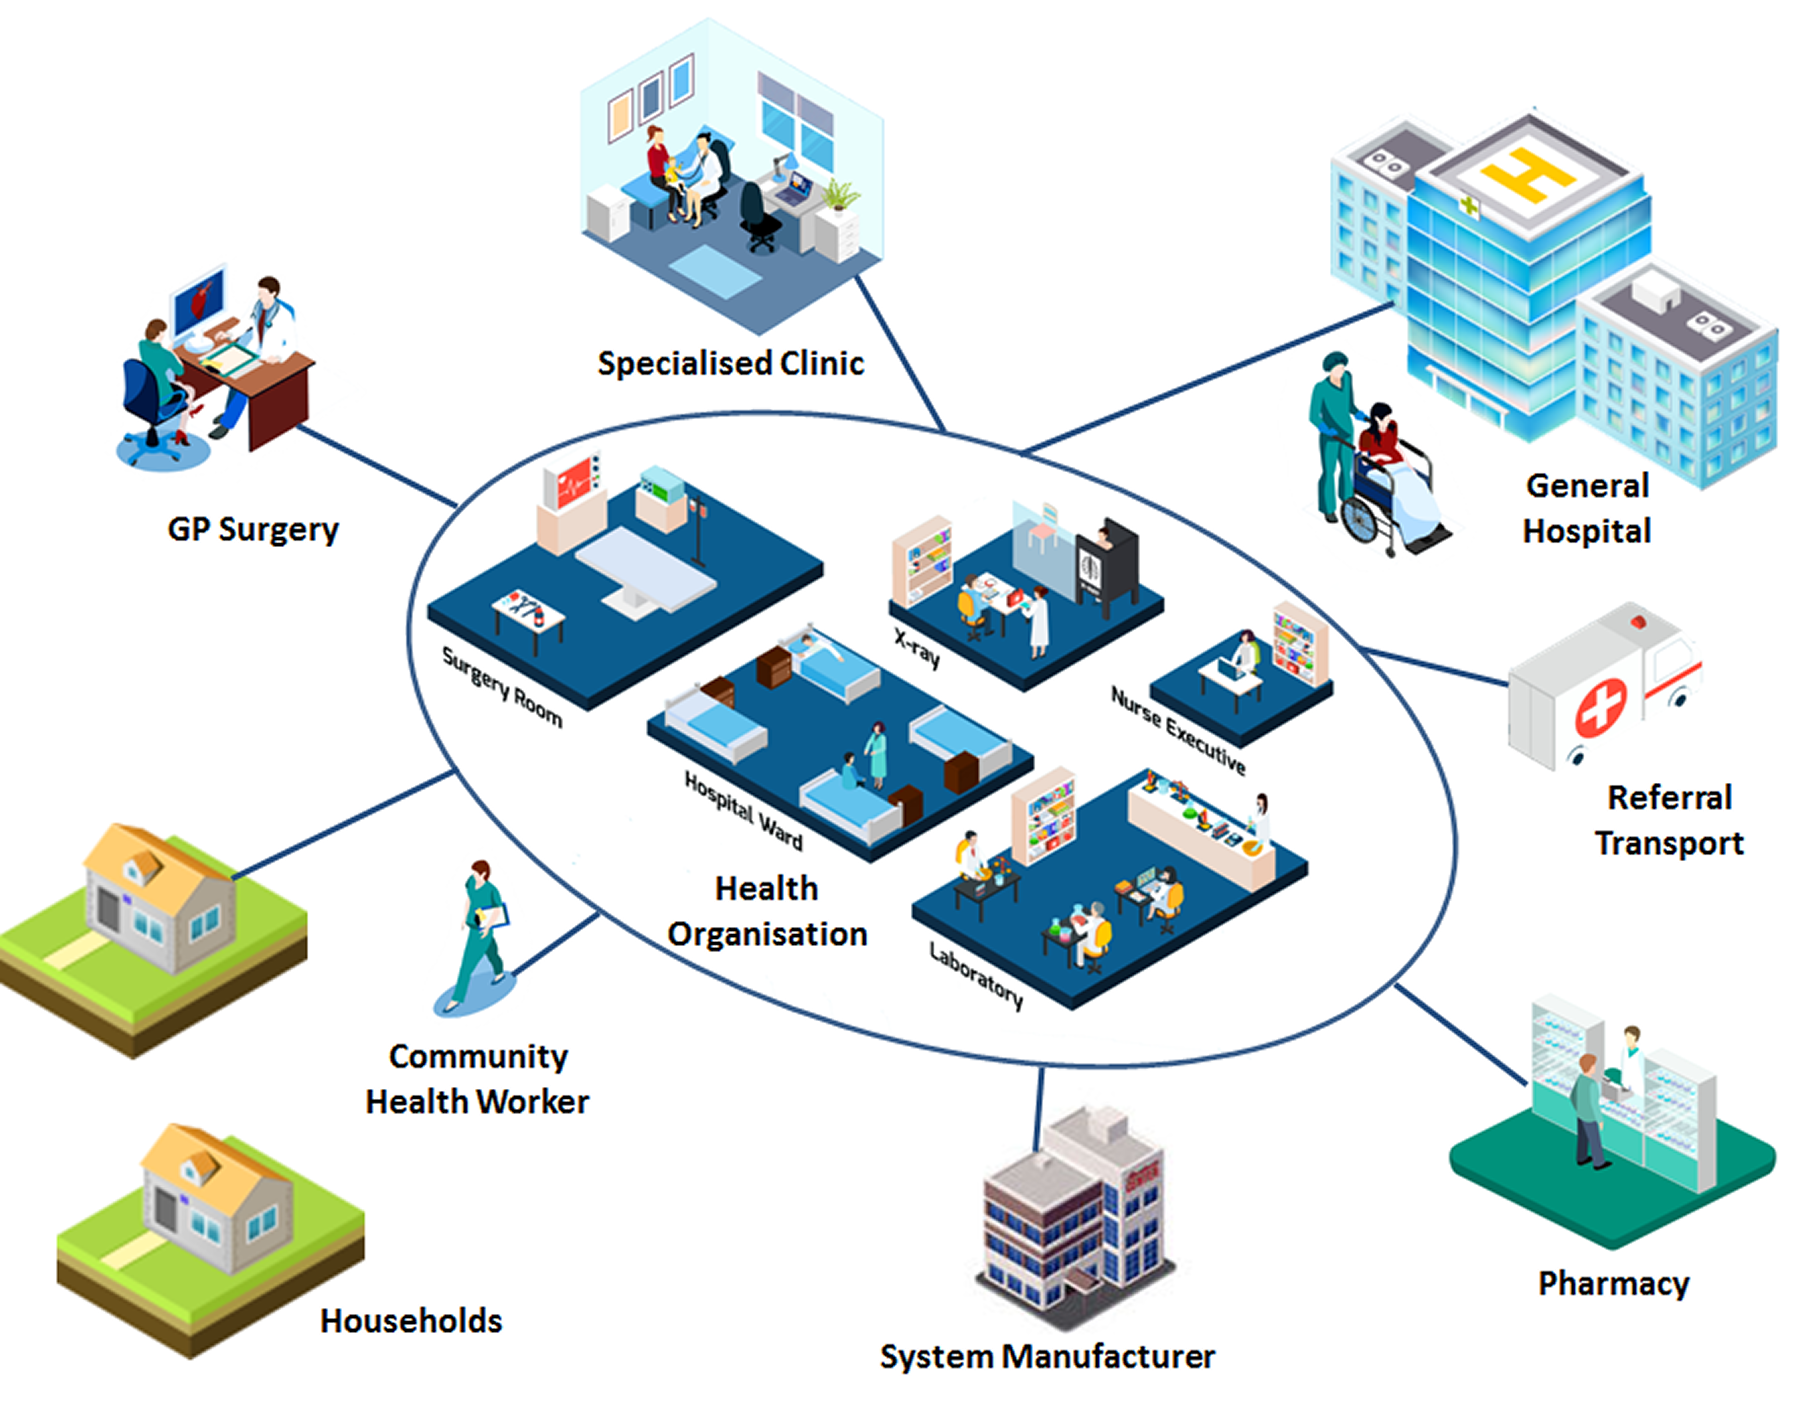
\includegraphics[width=0.9\textwidth]{images/medicalscenario}
  \label{fig:medicalscenario}
\end{figure}

\clearpage
The system is being targeted to meet the requirements of a Health Organization who are procuring a solution to help their clinicians maintain a high level of quality of care in the face of increasing volumes of patients and pressure to reduce staff costs.

From a data perspective, fundamental to fulfilling these requirements is establishing the context within which the use of data in system development, enhancement, introduction, integration or operation is occurring. This should establish the risk appetite: essentially, how much effort is devoted to making data risks as low as practicable. In turn, this will inform the nature and scope of assessments that are conducted during system development and, furthermore, its introduction into operational service. To meet the `Establish Context' objectives set out in the guidance the following activities are recommended:

\begin{itemize}
	\item Describe the organizational context;
	\item Describe the system context;
	\item Plan the assessment; and
	\item Identify Data Artefacts.
\end{itemize}

%
%Put text and image next to each other on the page.
%There are a number of ways of doing this, none of which are that nice or work that well.
%We could use the 'wrapfig' package but it's prone to errors in placement and running outside of page boundaries
%
\begin{minipage}[t][2cm]{0.73\textwidth}
  The Manufacturer decides to use an \gls{odr} Assessment form to understand in broad terms the level of risk it will have to manage in developing and supporting this system. This will allow the Manufacturer to \dsiwgTextBF{\dsiwgTextIT{Describe the organizational context}} and \dsiwgTextBF{\dsiwgTextIT{Describe the system context.}}
\end{minipage}
\begin{minipage}[c][1cm]{0.25\textwidth}
	\vspace{1cm}
  \centering
    
\includegraphics[width=\textwidth]{images/manufacturer}
\end{minipage}

\subsubsection{\Gls{odr} Assessment}
The Manufacturer considered each of the questions within the \gls{odr} form, which is presented in \autoref{bkm:assessment} of this document.
The following list identifies the questions in the \gls{odr} along with the assessments for the Manufacturer's system.

\begin{longtable*}[H]
  {|L{\dsiwgColumnWidth{0.06}}|L{\dsiwgColumnWidth{0.94}}|}
  \hline
  Q1: & How severe could an accident be that is related to the data? Could it be caused directly by the data?\\
  \hline
\end{longtable*}

Failings in the system could give rise to non-optimal \index{Treatment!Medical}treatment plans for a patient that might delay detection of a more serious condition or prolong the recovery for a known condition. The system is not solely relied upon however, and there are other people and systems in play involved in checking data. On balance, this question is assessed as: \dsiwgTextBF{1c}; Score \dsiwgTextBF{4}.

\begin{longtable*}[H]
  {|L{\dsiwgColumnWidth{0.06}}|L{\dsiwgColumnWidth{0.94}}|}
  \hline
  Q2: & What would be the impact on the organization, client or public if an accident occurred related to the data?\\
  \hline
\end{longtable*}

Unfortunately, accidents in the health domain are relatively frequent. There are many injuries and deaths attributed to medical errors but these are largely tolerated by the public and grievances are usually settled through financial settlements through the courts. The Manufacturer believes through their contractual arrangements that the Health Organization would be liable for any claims even if it was attributed to an error in the Manufacturer's system's handling of data. On balance, this question is assessed as: \dsiwgTextBF{2b}; Score \dsiwgTextBF{2}.

\clearpage %Manual page break
\begin{longtable*}[H]
  {|L{\dsiwgColumnWidth{0.06}}|L{\dsiwgColumnWidth{0.94}}|}
  \hline
  Q3: & How much responsibility does this organization have for data safety?\\
  \hline
\end{longtable*}

The Manufacturer is responsible for building the system in compliance with
DCB0129 \cite{citation:dcb0129clinical}
and so is responsible for executing the associated safety management system to manage risk. The Manufacturer however plans to sell the product with a condition of use that places end responsibility for patient safety on the client. On balance, this is question is assessed as: \dsiwgTextBF{3b}; Score \dsiwgTextBF{2}.

\begin{longtable*}[H]
  {|L{\dsiwgColumnWidth{0.06}}|L{\dsiwgColumnWidth{0.94}}|}
  \hline
  Q4: & What legal and regulatory environment will this work be subject to?\\
  \hline
\end{longtable*}

The work will be contracted under UK law and subject to the
\gls{dcb}
standards for Health IT Systems. However, there is no special regulator who is currently empowered to intervene in the delivery of healthcare systems, i.e., the standards are not currently enforced through law. The Health Organization however will make compliance with the standards a contractual requirement. On balance, this question is assessed as: \dsiwgTextBF{4c}; Score \dsiwgTextBF{4}.

\begin{longtable*}[H]
  {|L{\dsiwgColumnWidth{0.06}}|L{\dsiwgColumnWidth{0.94}}|}
  \hline
  Q5: & How mature is this organization regarding data safety?\\
  \hline
\end{longtable*}

The Manufacturer has a good understanding of data as a source of safety risk. Many of their systems are data intensive to support clinical decision making. There is good support and funding for the identification and resolution\index{Resolution Of Risks} of data-related risks. On balance, this question is assessed as: \dsiwgTextBF{5b}; Score \dsiwgTextBF{2}.

\begin{longtable*}[H]
  {|L{\dsiwgColumnWidth{0.06}}|L{\dsiwgColumnWidth{0.94}}|}
  \hline
  Q6: & How widely used is the data and who by?\\
  \hline
\end{longtable*}

The data will be used in multiple clinical settings and by many clinicians and other support staff. There are several data supply chains and public web access to data. On balance, this question is assessed as: \dsiwgTextBF{6c}; Score \dsiwgTextBF{4}.

\begin{longtable*}[H]
  {|L{\dsiwgColumnWidth{0.06}}|L{\dsiwgColumnWidth{0.94}}|}
  \hline
  Q7: & What is the scale, sophistication and complexity of the data and its manipulation?\\
  \hline
\end{longtable*}

The data is complex and although transmitted through industry standard data structures, these require knowledge of the associated abstract clinical data model. Some data manipulations are required to map between different encodings for data held in the various heterogeneous systems. Some legacy systems transfer data in unstructured format. On balance, this question is assessed as: \dsiwgTextBF{7c}; Score \dsiwgTextBF{4}.

\begin{longtable*}[H]
  {|L{\dsiwgColumnWidth{0.06}}|L{\dsiwgColumnWidth{0.94}}|}
  \hline
  Q8: & How well defined and understood are the boundaries and interfaces for this data scenario?\\
  \hline
\end{longtable*}

The boundaries of the supply are well understood and although the interfaces are complex and mixed formats, these will be defined and agreed formally through \glspl{icd}. Most of the integrating systems are established \gls{cots} based systems but some of the legacy systems still need to be investigated and working assumptions have been
made
by the Manufacturer. On balance, this question is assessed as: \dsiwgTextBF{8c}; Score \dsiwgTextBF{4}.

The final score is \dsiwgTextBF{26}, which corresponds to \dsiwgTextBF{ODR2}. The Manufacturer therefore concludes that there is low to medium risk that loss of \index{Property!Data}properties of data in the system can contribute to or give rise to harm. The Manufacturer has an internal policy for engagements based on the \gls{odr} level that dictates how the organization shall \dsiwgTextBF{\dsiwgTextIT{Plan the assessment}}; this policy dictates the amount of proportional effort it needs to spend on safety data management and the level of rigour to be employed. In this case, the policy dictates, amongst other requirements, that a separate section covering Safety Data Management is required in its Clinical Risk Management Plan.

The Manufacturer aims now to \dsiwgTextBF{\dsiwgTextIT{Identify Data Artefacts}} that are potential sources of safety hazards. The Manufacturer also knows that the safety dependency of data is dictated by the context in which it is used so it now develops an understanding of when in its process lifecycle\index{Lifecycle!Process} the data will be used and relied upon. The Manufacturer plans to build an early prototype to show to clients to help elicit requirements definition. To support this, the Manufacturer plans to create a test data set that comprises a typical range of scenarios that the system will encounter. This form of data is identified as \dsiwgTextBF{Verification Data}. The system also needs to be configured to support deploying Health Organizations' policies. This data is \dsiwgTextBF{Infrastructure Data}\index{Infrastructure Data} and, for the prototyping phase, the Manufacturer plans to use largely default values.

In later phases when the system functionality is specified and the system is being built, the Manufacturer plans to create a test data set that will be key to demonstrating the correct functioning of the system and hence acceptance by the deploying Health Organization. This still involves the use of \dsiwgTextBF{Verification Data}\index{Verification Data} and \dsiwgTextBF{Infrastructure Data}\index{Infrastructure Data} but there will be far greater dependency on these data sets than the prototyping case. The Manufacturer therefore documents the planned use of each of the data categories\index{Category!Data} during the entire delivery lifecycle\index{Lifecycle!Delivery} in the Clinical Risk Management Plan.

\begin{minipage}[t]{0.73\textwidth}
	The procuring Health Organization will have a different perspective of the IT system that they will deploy into their organization. They will already have many integrated systems in live operation and as part of establishing the context for the system's deployment they will need to consider many different types of data sets:
\end{minipage}
\begin{minipage}[t]{0.25\textwidth}
  \centering\raisebox{\dimexpr \topskip-\height}{%
    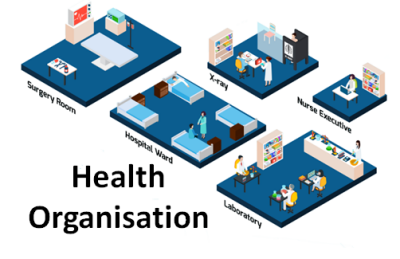
\includegraphics[width=\textwidth]{images/healthorganisation}}
\end{minipage}
	\begin{itemize}
		\item \dsiwgTextBF{Infrastructure Data}\index{Infrastructure Data}: how the system will be configured in the specific environment;
		\item \dsiwgTextBF{Verification Data}\index{Verification Data}: the test data sets to be used to support certain deployments such as integration testing and training; and
		\item \dsiwgTextBF{Dynamic Data}\index{Dynamic Data}: the data entered or fed into the system and the data presented to the user, generated in the form of reports or data passed to other systems.
	\end{itemize}

The Health Organization decides to complete an \gls{odr} assessment
so it can \dsiwgTextBF{\dsiwgTextIT{Describe the organizational context}} and \dsiwgTextBF{\dsiwgTextIT{Describe the system context}}. The scoring is similar to the Manufacturer with the following notable differences:

\begin{longtable*}[H]
  {|L{\dsiwgColumnWidth{0.06}}|L{\dsiwgColumnWidth{0.94}}|}
  \hline
  Q2: & What would be the impact on the organization, client or public if an accident occurred related to the data?\\
  \hline
\end{longtable*}

The Health Organization would bear the brunt of any publicity and litigation in the event of an accident and so assess this question as \dsiwgTextBF{2c}, Score \dsiwgTextBF{4}.

\begin{longtable*}[H]
  {|L{\dsiwgColumnWidth{0.06}}|L{\dsiwgColumnWidth{0.94}}|}
  \hline
  Q3: & How much responsibility does this organization have for data safety?\\
  \hline
\end{longtable*}

The Health Organization is responsible for deploying systems in compliance with
DCB0160 \cite{citation:dcb0160clinical}
and is ultimately responsible for patient safety. The Health Organization assesses this as \dsiwgTextBF{3e}, Score \dsiwgTextBF{12}.

\begin{longtable*}[H]
  {|L{\dsiwgColumnWidth{0.06}}|L{\dsiwgColumnWidth{0.94}}|}
  \hline
  Q5: & How mature is this organization regarding data safety?\\
  \hline
\end{longtable*}

The Health Organization has only recently acquired the expertise to apply
DCB0160
and is still developing its capability. Safety Data Management is new to the organization and it anticipates some resistance from senior management after the expenditure incurred in rolling out a
DCB0160
compliant safety management system. This question is assessed as \dsiwgTextBF{5d}, Score \dsiwgTextBF{7}.

The resulting score for the Health Organization is \dsiwgTextBF{43}. This is \dsiwgTextBF{ODR3}; medium to high risk.
The Health Organization aims to \dsiwgTextBF{\dsiwgTextIT{Plan the assessment}} through a Clinical Risk Management Plan. This plan defines the organization and system context in more detail and lays out the planned activities for identifying, evaluating and treating data safety related risks.

As with the Manufacturer, the Health Organization needs to \dsiwgTextBF{\dsiwgTextIT{Identify Data Artefacts}} that are potential sources of safety hazards and understand the context of their use in the procurement / deployment lifecycles of the Health Organisation\index{Lifecycle}.
Post acceptance, the procuring Health Organization plans to run a series of user training sessions for clinicians.
Once users are trained, the system will be integrated into live operations.
The Health Organization identifies the Infrastructure\index{Infrastructure Data},
Verification\index{Verification Data} and Dynamic\index{Dynamic Data} Data Categories to be used
during these phases.
The Health Organization also realises that the system will form part of a data supply chain as a number of external organizations and departments within their own organization engage in the procurement and use of safety-related data.
For example, it will receive referral data from a number of other \gls{gp} systems, it will receive outcome measures from hospitals and clinical data acquired from remote workers visiting patients in the community and also from the patients themselves using the system's online portal.
The system also produces data for other external systems such as electronic prescriptions for pharmacies.

The Health Organization sees that by using the new system it will become a Commissioning User as it will require and be a \dsiwgTextBF{Consumer} of data from a variety of sources; these sources are: \gls{gp}'s systems, hospital systems, systems used by remote workers in the community and the system's portal capturing data entered by the patients themselves, each of these acting as \dsiwgTextBF{Data Provisioners}. Those health care professionals (and the patient themselves) gathering patient data through physical inspections and measurement are the \dsiwgTextBF{Data Acquirers}.

The Health Organization defines the data supply chain relevant to the system including the roles and interfaces involved in its Clinical Risk Management Plan. This will therefore show where there are dependencies on \dsiwgTextBF{Dynamic Data} used and produced by the system.

Questions the Health Organization will need to address when establishing the context are:
\begin{itemize}
  \item Have all the dependent interfaces been identified?
  \item Have the roles of Commissioning User / Data Provider / Data Acquirer been established and acknowledged?
  \item What `service levels' or contracts exist for the delivery of the data?
  \item What level of assurance do Data Providers/Data Acquirers provide for their data?
\end{itemize}

\subsection{Risk Identification}
\begin{minipage}[t]{0.73\textwidth}
  The Manufacturer aims to carry out the following activities to meet the guidance objectives for the Risk Identification phase.
  \begin{itemize}
    \item Review the general, historical perspective;
    \item Conduct a top-down approach;
    \item Conduct a bottom-up approach; and
    \item Update planning documents.
  \end{itemize}
\end{minipage}
\begin{minipage}[t]{0.25\textwidth}
  \centering\raisebox{\dimexpr \topskip-\height}{%
    
\includegraphics[width=\textwidth]{images/manufacturer}}
\end{minipage}

Before embarking on any hazard analysis, the Manufacturer ensures that \index{Stakeholder}Stakeholders \dsiwgTextBF{\dsiwgTextIT{Review the general, historical perspective}}. This takes the form of a refresh briefing to raise awareness of issues that are specific to data such as ageing, biasing and defaults.

The Manufacturer of the Health IT System decides that during the prototyping phase there is little safety dependency of the test and \gls{configuration data} sets as no clinical decisions will be made based on their content; the data is simply being used to support the elaboration of requirements.

In later phases however, when the system functionality is specified and the system is being built, the Manufacturer will want to create a test data set that will be instrumental in demonstrating the correct functioning of the system. This still involves the use of \dsiwgTextBF{Verification Data}\index{Verification Data} and \dsiwgTextBF{Infrastructure Data}\index{Infrastructure Data} but there is far greater dependency on these data sets than the previous case. For example, if the verification or \gls{configuration data} is not sufficiently diverse or insufficiently models real-world scenarios, it is possible that erroneous and unsafe functional behaviour is present in the system during live operation despite this system having passed factory and site acceptance testing.

To analyse the risks in more detail the Manufacturer uses a \dsiwgTextBF{\dsiwgTextIT{Top-down approach}} and a \dsiwgTextBF{\dsiwgTextIT{Bottom-up approach}}. In the first approach it considers each of the system functions (such as clinical screens) and analyses where there is a dependency on data and the \index{Property!Data}properties that need to be preserved. In the second, as much of the functionality is driven by data flows in and out of the system, the Manufacturer also looks at specific data flows and assesses the impact if there are loss of \index{Property!Data}properties for the data in those flows.

On completion of the risk identification phase the Manufacturer \dsiwgTextBF{\dsiwgTextIT{Updates planning documents}} such as the Clinical Risk Management Plan to reflect the outcome of the analysis.

\begin{minipage}[t]{0.73\textwidth}
  The Health Organization will likewise need to conduct risk identification relevant to their deployment context. Hazards arising from data sources that are to be delivered into the new system from existing systems need to be assessed for data risks.
  As with the Manufacturer, a briefing to \index{Stakeholder}Stakeholders to \dsiwgTextBF{\dsiwgTextIT{Review the general, historical perspective}} is first conducted to cover generic data safety issues but also to highlight lessons learned from previous accidents and incidents that have occurred in the Health Organization itself.
\end{minipage}
\begin{minipage}[t]{0.25\textwidth}
  \centering\raisebox{\dimexpr \topskip-\height}{%
    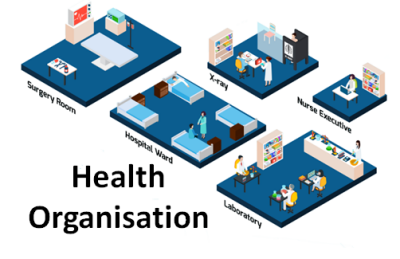
\includegraphics[width=\textwidth]{images/healthorganisation}}
\end{minipage}

As with the Manufacturer, both a \dsiwgTextBF{\dsiwgTextIT{Top-down approach}} and a \dsiwgTextBF{\dsiwgTextIT{Bottom-up approach}} is adopted. From the Health Organization's perspective, one key focus for hazard identification is in the use of \dsiwgTextBF{Dynamic Data}, i.e., data that will be delivered into the new system from existing system data sources, and the data presented to the user. For the interactions identified in the supply chain, the Health Organization needs to consider the risks associated with loss of \index{Property!Data}properties of the data it will receive. Questions the Health Organization will need to consider and address more formally in the Clinical Risk Management Plan are as follows:
\clearpage% Required on 3.3 to keep page breaks as 3.2
\begin{itemize}
  \item Which data sets or items being received from other systems have \index{Property!Data}Data Properties (such as timeliness\index{Timeliness Property}, \index{Completeness!Property}\gls{completeness}, \index{Consistency!Property}\gls{consistency}, \index{Fidelity/Representation Property}fidelity etc.) that are significant to patient safety? 
  \item What data presented to the user has \index{Property!Data}Data Properties (such as \index{Availability Property}\gls{availability}, format, resolution\index{Resolution Property}, etc.) that are significant to patient safety?
  \item What existing barriers or mitigations\index{Mitigation} (physical, technical, procedural) exist to reduce the risk of loss of \index{Property!Data}Data Properties?
  \item
  Will any existing barriers be lost as a consequence of the new system?
\end{itemize}

On completion of the Risk Identification phase the Health Organization will \dsiwgTextBF{\dsiwgTextIT{Update planning documents}} such as the Clinical Risk Management Plan to reflect the outcome of the analysis.

\subsection{Risk Analysis}
\begin{minipage}[t]{0.73\textwidth}
  In this phase identified hazards are assessed to determine their likelihood and severity. To meet the guidance objectives the following activities are carried out:
  \begin{itemize}
    \item Establish \glspl{dsal}\index{Assurance Level!Data}; and
    \item Analyse \glspl{dsal} as part of system safety activities.
  \end{itemize}
\end{minipage}
\begin{minipage}[t]{0.25\textwidth}
  \centering\raisebox{\dimexpr \topskip-\height}{%
    
\includegraphics[width=\textwidth]{images/manufacturer}}
\end{minipage}

The Manufacturer will \dsiwgTextBF{\dsiwgTextIT{Establish \glspl{dsal}\index{Assurance Level!Data}}} by considering cases where the use of specific categories of data\index{Category!Data} could give rise to hazards. In the first, the prototyping phase, the Manufacturer sees no use of the data that can give rise to credible clinical risk and assessing the \gls{dsal}\index{Assurance Level!Data} for that data set as \dsiwgTextBF{DSAL0}. 

In the second phase of the development lifecycle\index{Lifecycle!Development}, where \dsiwgTextBF{Verification Data}\index{Verification Data} and \dsiwgTextBF{Infrastructure Data}\index{Infrastructure Data} is being used to demonstrate the correct functioning of the system, the Manufacturer considers that loss of any of the Data Properties of \dsiwgTextBF{\index{Integrity Property}Integrity, \index{Completeness!Property}\gls{completeness}, \index{Consistency!Property}\gls{consistency}, \index{Continuity Property}\gls{continuity}, \index{Format Property}Format, \index{Accuracy Property}\gls{accuracy}, Resolution{Resolution! Data}, Timeliness\index{Timeliness Property}, \index{Availability Property}\gls{availability}, \index{Fidelity/Representation Property}Fidelity / Representation, Sequencing\index{Sequencing, Data}, Intended Destination / Usage\index{Intended Destination/Usage Property}, Goldilocks\index{Goldilocks Property}, Explainability\index{Explainability Property}} of this data could give rise to hazards.

For example, if the verification data set selected is not representative of the eventual diversity experienced in practice (loss of \index{Fidelity/Representation Property}Fidelity / Representation), then it is possible that the system may contain latent software errors that could give rise to harm. However, the Manufacturer acknowledges that the system will be subject to further testing and trials in the clinical setting and so there will be other opportunities to detect errors in the system. Overall:
\begin{itemize}
  \item The likelihood of the data use gives rise to an accident is \dsiwgTextBF{Medium} as other systems and processes are in place that would detect errors; and
  \item The severity is \dsiwgTextBF{Moderate}; failings in the system could give rise to non-optimal \index{Treatment!Medical}treatment plans for a patient that might delay detection of a more serious condition or prolong the recovery for a known condition.
\end{itemize}

The Manufacturer therefore assesses these data categories\index{Category!Data} as \dsiwgTextBF{DSAL1}\index{Assurance Level!Data} in this particular context of use.

The Manufacturer takes care to \dsiwgTextBF{\dsiwgTextIT{Analyse \glspl{dsal}\index{Assurance Level!Data} as part of system safety activities}} by documenting these assessments along with other hardware and software safety considerations, for example those arising from
DCB0129,
in the Clinical Risk Management Plan.

\begin{minipage}[t]{0.73\textwidth}
  From the Health Organization's perspective, the main focus for risk assessment to \dsiwgTextBF{\dsiwgTextIT{Establish \glspl{dsal}\index{Assurance Level!Data}}} is in the use of \dsiwgTextBF{\dsiwgTextIT{Dynamic Data}}\index{Dynamic Data}. For the interactions identified in the supply chain the Health Organization needs to consider the risks associated with loss of \index{Property!Data}properties of the data it will receive and present to the user. Questions the Health Organization will need to consider and address more formally in the Clinical Risk Management Plan are as follows:
\end{minipage}
\begin{minipage}[t]{0.25\textwidth}
  \centering\raisebox{\dimexpr \topskip-\height}{%
    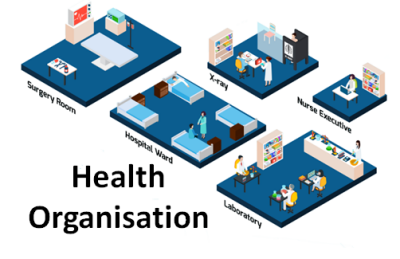
\includegraphics[width=\textwidth]{images/healthorganisation}}
\end{minipage}

\begin{itemize}
  \item How likely is it that there would be a loss of the given \index{Property!Data}Data Property?
  \item How would such a loss of a \index{Property!Data}Data Property be detected?
  \item How would such as loss be isolated to prevent further risks of harm?
  \item What recovery action would be required to resolve the issue to maintain patient safety?
\end{itemize}

Concerns were raised about the vulnerability of the system to inadvertent data overload from the large number of potential data sources, and possibly from malicious activity. This led to the addition of the \dsiwgTextBF{Goldilocks}\index{Goldilocks Property} property to the list of \index{Property!Data}Data Properties applicable to the live system.

In considering the receipt of outcome measures data received from a clinic or hospital, the Health Organization considers that it is likely that some credible errors would not be readily detected by their new system; if the hospital system confused a result or there were errors in the precision of data then there would be few chances to catch these once received by the system.
\begin{itemize}
  \item The Health Organizations assesses the likelihood of this loss of \index{Property!Data}property as \dsiwgTextBF{High}; and
  \item The impact of such errors, although not realistically likely to lead to death, could result in delays to \index{Treatment!Medical}treatment that could result in serious injury and hence \dsiwgTextBF{Moderate} impact.
\end{itemize}

The data received from this data source is therefore classed as \dsiwgTextBF{DSAL2}\index{Assurance Level!Data} in this particular context of use.

The Health Organization takes care to \dsiwgTextBF{\dsiwgTextIT{Analyse \glspl{dsal}}} as part of system safety activities by documenting these assessments along with other hardware and software safety considerations (e.g., arising from
DCB0160
requirements) in the Clinical Risk Management Plan.

\subsection{Risk Evaluation and \index{Treatment!Risk}Treatment}

\begin{minipage}[t]{0.73\textwidth}
  The Manufacturer carries out the following activities to meet the guidance objectives:
  \begin{itemize}
    \item Review each risk and either: Avoid; Accept; Transfer; Treat;
    \item Establish \index{Treatment!Risk} methods for relevant risks; and
    \item Implement and verify \index{Treatment!Risk}treatment methods.
  \end{itemize}
\end{minipage}
\begin{minipage}[t]{0.25\textwidth}
  \centering\raisebox{\dimexpr \topskip-\height}{%
    
\includegraphics[width=\textwidth]{images/manufacturer}}
\end{minipage}

The Manufacturer decides to \dsiwgTextBF{\dsiwgTextIT{Review each risk and either: Avoid; Accept; Transfer; or Treat the risk}}. It decides to \dsiwgTextBF{Accept} the \dsiwgTextBF{DSAL0}\index{Assurance Level!Data} risk but as it has determined there is some, albeit low, risk (\dsiwgTextBF{DSAL1}) associated with its use of data at a specific point of its lifecycle\index{Lifecycle!Data}, it decides to \dsiwgTextBF{Treat} that risk. The Manufacturer evaluates this risk and considers that the risks should be reduced further by taking some reasonably practicable steps.

Having decided that further risk reduction is necessary, the Manufacturer needs to \dsiwgTextBF{\dsiwgTextIT{Establish \index{Treatment!Risk}treatment methods for relevant risks}} that are appropriate for DSAL1\index{Assurance Level!Data}data and in doing so demonstrate that reasonably practicable steps have been taken to reduce the risk. The Manufacturer therefore refers to the tables in the \gls{dsg} document. The Manufacturer then documents in its Clinical Risk Management Plan:

\begin{itemize}
  \item Planned compliance with the tables;
  \item The interpretation for the given method/technique (e.g.\ depth of checking); and
  \item Justification in the case where a technique is not to be adopted.
\end{itemize}

For \dsiwgTextBF{DSAL1}\index{Assurance Level!Data} Verification Data, the tables show that the following are recommended (R) or highly recommended (HR) where loss of Data Properties \dsiwgTextBF{\index{Integrity Property}Integrity, \index{Completeness!Property}\gls{completeness}, \index{Consistency!Property}\gls{consistency}, \index{Continuity Property}\gls{continuity}, \index{Format Property}Format, \index{Accuracy Property}\gls{accuracy}, Resolution{Resolution! Data}, Timeliness\index{Timeliness Property}, \index{Availability Property}\gls{availability}, \index{Fidelity/Representation Property}Fidelity / Representation, Sequencing\index{Sequencing, Data}, Intended Destination / Usage\index{Intended Destination/Usage Property}, Goldilocks\index{Goldilocks Property}, Explainability\index{Explainability Property}} can give rise to
a number of hazards. The extracts below indicate the mitigation\index{Mitigation} techniques identified from the tables which should form the basis of the \index{Safety Requirement!Data}data safety requirements. 

\begin{longtable}{|C{\dsiwgColumnWidth{0.08}}|L{\dsiwgColumnWidth{0.15}}|C{\dsiwgColumnWidth{0.08}}|L{\dsiwgColumnWidth{0.69}}|}
  \caption{Worked example: Filtered Techniques tables}
  \\\hline\TableHeadColourC{Ref} & \TableHeadColour{Technique} & \TableHeadColourCX{R/HR} & \TableHeadColour{System Design
  \hfill(extracted from \autoref{tab:MethodsSystemDesign})
  }\\\hline
  \endfirsthead
  \caption[]{Worked example: Filtered Techniques tables (continued)}
  \\hline\TableHeadColourC{Ref} & \TableHeadColour{Technique} & \TableHeadColourCX{R/HR} & \TableHeadColour{System Design}\\\hline
  \endhead
  \multicolumn{4}{r}{\sl Continued on next page}
  \endfoot\endlastfoot
  SD.11 & Logging Facilities & R & Data processing events are logged to allow support staff to monitor the health of the system and provide diagnostic information.
  \\
  \hline
  SD.17 & Sanity / Reasonability Checks & R & Dedicated processing implemented to check that data is within reasonable tolerances and / or logically / semantically consistent (e.g., range checks, date checks, record counts, record sizes, special values - \gls{nan}). \\
  \hline
  SD.20 & Syntax Checks & R & Semantic checking of data values and sequences based on defined rule sets.\\
  \hline
\end{longtable}

\begin{longtable*}{|C{\dsiwgColumnWidth{0.08}}|L{\dsiwgColumnWidth{0.15}}|C{\dsiwgColumnWidth{0.08}}|L{\dsiwgColumnWidth{0.69}}|}
  \hline\TableHeadColourC{Ref} & \TableHeadColour{Technique} & \TableHeadColourC{R/HR} & \TableHeadColour{Data Design
  \hfill(extracted from \autoref{tab:MethodsDataDesign})
  }\\\hline
  \endfirsthead
  \hline\TableHeadColourC{Ref} & \TableHeadColour{Technique} & \TableHeadColourC{R/HR} & \TableHeadColour{Data Design}\\\hline
  \endhead
  \endfoot\endlastfoot
  DD.01 & Governance Model & R & A governance model is established that defines, e.g., \index{Data!Owner}data ownership, processing roles and responsibilities, processing authorizations and permissions.\\
  \hline
  DD.03 & Data Flow Diagram & HR & To describe the data flow in a diagrammatic form.\\
  \hline
  DD.04 & Data Model & HR & To articulate how data is organized.\\
  \hline
  DD.05 & Client Sign-off & R & \cbstart Agreement from the client that the system architecture and design is appropriate for the data considered\cbend \\
  \hline
  DD.08 & Data Dictionary & HR & A collection of descriptions of the data objects or items in a data model for the benefit of data users.\\
  \hline
\end{longtable*}

\begin{longtable*}{|C{\dsiwgColumnWidth{0.08}}|L{\dsiwgColumnWidth{0.15}}|C{\dsiwgColumnWidth{0.08}}|L{\dsiwgColumnWidth{0.69}}|}
  \hline\TableHeadColourC{Ref} & \TableHeadColour{Technique} & \TableHeadColourC{R/HR} & \TableHeadColour{Data Implementation
  \hfill(extracted from \autoref{tab:MethodsDataProcedures})
  }\\\hline
  \endfirsthead
  \hline\TableHeadColourC{Ref} & \TableHeadColour{Technique} & \TableHeadColourC{R/HR} & \TableHeadColour{Data Implementation}\\\hline
  \endhead
  \endfoot\endlastfoot
   DI.01 & Review / Inspection & HR & Manual review / inspection of data possibly involving data visualization tools.\\
  \hline
   DI.03 & Ground-Truth Check & R & Inspection against physical measurements (e.g., lengths, positions, heights) taken in the real world.\\
  \hline
   DI.04 & Auditing & R & A period of comprehensive internal and external testing of the data quality process.\\
  \hline
   DI.09 & Authorization & R & A security model is established to control who is authorized to create, view, edit, delete the data.\\
  \hline
   DI.11 & Defined Confidence / Trust Levels & R & Criteria are established to provide an objective measurement of the confidence or trust in a given data set.\\
  \hline
\end{longtable*}

\begin{longtable*}{|C{\dsiwgColumnWidth{0.08}}|L{\dsiwgColumnWidth{0.15}}|C{\dsiwgColumnWidth{0.08}}|L{\dsiwgColumnWidth{0.69}}|}
  \hline\TableHeadColourC{Ref} & \TableHeadColour{Technique} & \TableHeadColourC{R/HR} & \TableHeadColour{Data Migration
  \hfill(extracted from \autoref{tab:MethodsDataMigration})
  }\\\hline
  \endfirsthead
  \hline\TableHeadColourC{Ref} & \TableHeadColour{Technique} & \TableHeadColourC{R/HR} & \TableHeadColour{Data Migration}\\\hline
  \endhead
  \endfoot\endlastfoot
  \multicolumn{4}{|l|}{No relevant techniques}\\
  \hline
\end{longtable*}

\begin{longtable*}{|C{\dsiwgColumnWidth{0.08}}|L{\dsiwgColumnWidth{0.15}}|C{\dsiwgColumnWidth{0.08}}|L{\dsiwgColumnWidth{0.69}}|}
  \hline\TableHeadColourC{Ref} & \TableHeadColour{Technique} & \TableHeadColourC{R/HR} & \TableHeadColour{Data Checking
  \hfill(extracted from \autoref{tab:MethodsDataChecking})
  }\\\hline
  \endfirsthead
  \hline\TableHeadColourC{Ref} & \TableHeadColour{Technique} & \TableHeadColourC{R/HR} & \TableHeadColour{Data Checking}\\\hline
  \endhead
  \endfoot\endlastfoot
  \multicolumn{4}{|l|}{No relevant techniques}\\
  \hline
\end{longtable*}

\begin{longtable*}{|C{\dsiwgColumnWidth{0.08}}|L{\dsiwgColumnWidth{0.15}}|C{\dsiwgColumnWidth{0.08}}|L{\dsiwgColumnWidth{0.69}}|}
  \hline\TableHeadColourC{Ref} & \TableHeadColour{Technique} & \TableHeadColourC{R/HR} & \TableHeadColour{Test Data
  \hfill(extracted from \autoref{tab:MethodsTestData})
  }\\\hline
  \endfirsthead
  \hline\TableHeadColourC{Ref} & \TableHeadColour{Technique} & \TableHeadColourC{R/HR} & \TableHeadColour{Test Data}\\\hline
  \endhead
  \endfoot\endlastfoot
   TD.01 & Using Informal / Ad-hoc Means & R & Data is generated by simple means (e.g, spreadsheets, scripts, basic assumptions). There is no formal checking or review of the method of generation.\\
  \hline
   TD.05 & Using Manual Means & R & Simple test data can be produced by manual means, although this may be prone to human error.\\
  \hline
   TD.08 & Using Initial Runs of New System & R & This method is often used where the system is breaking new ground and there is no prototype or legacy system to produce test data. Initial operations may differ from eventual usage, so test data must evolve.\\
  \hline
   TD.09 & Derived from Real Data & R & Where real data is available this is usually a good basis for generating test data (e.g., by modification to increase the test space coverage).\\
  \hline
   TD.11 & Produced by Client & R & Ideally the client is involved in producing or at least checking the test data.\\
  \hline
   TD.12 & Client Sign-off & R & Where possible, the client should formally agree and sign off the test data as appropriate.\\
  \hline
   TD.13 & Error Seeding & R & This is where errors are deliberately inserted into the data set to demonstrate the effectiveness of data validation.\\
  \hline
   TD.14 & Data Reuse & R & Reusing data for one project that was created and thoroughly assured for another project. This can be effective but the read-across should be established.\\
  \hline
   TD.15 & Feedback Testing & R & To check output data by comparing it with the input source.\\
  \hline
\end{longtable*}

\begin{longtable*}{|C{\dsiwgColumnWidth{0.08}}|L{\dsiwgColumnWidth{0.15}}|C{\dsiwgColumnWidth{0.08}}|L{\dsiwgColumnWidth{0.69}}|}
  \hline\TableHeadColourC{Ref} & \TableHeadColour{Technique} & \TableHeadColour{R/HR} & \TableHeadColour{Media - Paper
  \hfill(extracted from \autoref{tab:MethodsDataMediaPhysical})
  }\\\hline
  \endfirsthead
  \hline\TableHeadColourC{Ref} & \TableHeadColour{Technique} & \TableHeadColour{R/HR} & \TableHeadColour{Media - Paper}\\\hline
  \endhead
  \endfoot\endlastfoot
  MP.01 & Photographic Copies & R & Photocopy and store separately.\\
  \hline
  MP.02 & Scan to Electronic Format & R & Retain both paper and electronic copies.\\
  \hline
  MP.10 & Indexing / Cataloguing & R & To support efficient accessibility.\\
  \hline
\end{longtable*}

\begin{longtable*}{|C{\dsiwgColumnWidth{0.08}}|L{\dsiwgColumnWidth{0.15}}|C{\dsiwgColumnWidth{0.08}}|L{\dsiwgColumnWidth{0.69}}|}
  \hline\TableHeadColourC{Ref} & \TableHeadColour{Technique} & \TableHeadColourC{R/HR} & \TableHeadColour{Media - Electronic
  \hfill(extracted from \autoref{tab:MethodsDataMediaElectronic})
  }\\\hline
  \endfirsthead
  \hline\TableHeadColourC{Ref} & \TableHeadColour{Technique} & \TableHeadColourC{R/HR} & \TableHeadColour{Media - Electronic}\\\hline
  \endhead
  \endfoot\endlastfoot
   ME.01 & Regular Refresh / Rewrite & R & Of magnetic media or flash memory.\\
  \hline
   ME.02 & Suitable Physical Environment & R & Store media in a clean, low-humidity environment at a steady temperature, cool but not cold.\\
  \hline
   ME.03 & Copies at Different Locations & R & Physically separate to cover natural disasters, accidental or malicious damage.\\
  \hline
   ME.04 & Backups / Duplication & R & Backups are essential. Frequency of backup depends on rate of change. The number of generations to keep relates to the impact of data loss.\\
  \hline
   ME.05 & Sample Restores & R & Sample restores should be performed at intervals to ensure that the backups are readable and retrievable.\\
  \hline
\end{longtable*}

From these tables the Manufacturer decides on a series of activities to implement the recommendations that are applicable to its particular endeavour. These activities are expressed as a series of requirements that can be placed on the Manufacturer's delivery organization and tracked through to completion. 

\begin{longtable}{|C{\dsiwgColumnWidth{0.07}}|L{\dsiwgColumnWidth{0.78}}|C{\dsiwgColumnWidth{0.15}}|}
\caption{Worked example: Derived \index{Safety Requirement!Data!Derived}data safety requirements}
  \\\hline\TableHeadColourC{} & \TableHeadColour{} & \TableHeadColourCX{Guidance}\\
  \multirow{-2}*{\TableHeadColourC{Ref}} & \multirow{-2}*{\TableHeadColour{Requirement}} & \TableHeadColourCX{Reference}\\\hline
  \endfirsthead
    \caption[]{Worked example: Derived \index{Safety Requirement!Data!Derived}data safety requirements (continued)}
  \\\hline\TableHeadColourC{} & \TableHeadColour{} & \TableHeadColourCX{Guidance}\\
  \multirow{-2}*{\TableHeadColourC{Ref}} & \multirow{-2}*{\TableHeadColour{Requirement}} & \TableHeadColourCX{Reference}\\\hline
  \endhead
      \multicolumn{3}{r}{\sl Continued on next page}
\endfoot\endlastfoot
  R1 & The verification data shall be carefully controlled in the Manufacturer's configuration management system. There shall be a configuration management plan that shall define who has responsibility for the data and who is authorized to create and amend it. & DD.01, DI.09\\
  \hline
  R2 & The verification data shall be held on an industry standard file share that is regularly backed up with copies moved periodically to off-site storage. The Backup / Recovery plans shall include periodic sampling of restores. & ME.01, ME.02, ME.03, ME.04, ME.05\\
  \hline
  R3 & The data shall be modelled as a series of patient ``journeys'' that cover the entire lifecycle\index{Lifecycle!Data} of data from first encounter through to archival and deletion of data. The complete set of journeys shall be chosen to exercise all the functionality of the system. The modelling shall include a data dictionary, data flow diagrams and a data model. & DD.03, DD.04, DD.08\\
  \hline
  R4 & To model data from external systems, the Manufacturer shall use manual data entry\index{Data!Entry} and spreadsheet based records to hold the data. & TD.01, TD.05\\
  \hline
  R5 & The Manufacturer has a set of clinical standing data that was used for another system and derived from real data.
  It includes encounter codes, clinical terms, consultant names, surgery and hospital addresses etc.\ and can be reused for this system. The Manufacturer's Clinical Safety Officer has reviewed the data and agreed its suitability for reuse. & TD.09, TD.14\\
  \hline
  R6 & Some of the verification data sets shall include errors deliberately inserted to check the effectiveness of data validation. & TD.13\\
  \hline
  R7 & The controlled verification data set shall be subject to review and analysis against defined confidence/trust criteria. Scripts shall be written to check for syntax and semantic \index{Consistency!Semantic}\gls{consistency} of the data and provide a basic sanity check. The scripts themselves shall be validated and verified before use. & SD.17, SD.20, DI.01, DI.03, DI.11\\
  \hline
  R8 & The project shall be subject to an internal delivery quality assurance audit. & DI.04\\
  \hline
  R9 & Data loaded from external system into the system and displayed to the user shall be crosschecked against the original source data, using manual spot-checks. & TD.15\\
  \hline
  R10 & The level of rigour employed in verifying all the above requirements shall be commensurate with the \gls{dsal}\index{Assurance Level!Data} \gls{criticality} and so an ISO9001 compliant quality management system shall be adopted. & All\\
  \hline
  R11 & Data processing events shall be logged to allow monitoring of the health of the system, provide diagnostic information, allow audit trails and support the production of explanations. & SD.11
  \\
  \hline
\end{longtable}

The following guidance recommendations were not adopted by the Manufacturer for the reasons given. Note that some may however become relevant in the future so actions are set, where appropriate, to review the applicability of the recommendation when the given condition is met.

\begin{longtable}{|C{\dsiwgColumnWidth{0.07}}|C{\dsiwgColumnWidth{0.13}}|L{\dsiwgColumnWidth{0.55}}|L{\dsiwgColumnWidth{0.25}}|}
\caption{Worked example: \index{Safety Requirement!Data!Rejected}Rejected data safety requirements}
  \\\hline\TableHeadColourC{} & \TableHeadColourC{Guidance} & \TableHeadColour{} & \TableHeadColourCX{}\\
  \multirow{-2}*{\TableHeadColourC{Ref}} & \TableHeadColourC{Reference} & \multirow{-2}*{\TableHeadColour{Justification}} & \multirow{-2}*{\TableHeadColourCX{Action}}\\\hline
  \endfirsthead
\caption[]{Worked example: \index{Safety Requirement!Data!Rejected}Rejected data safety requirements (continued)}
  \\\hline\TableHeadColourC{} & \TableHeadColourC{Guidance} & \TableHeadColour{} & \TableHeadColourCX{}\\
  \multirow{-2}*{\TableHeadColourC{Ref}} & \TableHeadColourC{Reference} & \multirow{-2}*{\TableHeadColour{Justification}} & \multirow{-2}*{\TableHeadColourCX{Action}}\\\hline
  \endhead
      \multicolumn{4}{r}{\sl Continued on next page}
  \endfoot\endlastfoot
  E1 & TD.08 & The data will be used before any initial run of the system. & Review when data from initial runs is available.\\
  \hline
  E2 & DD.05, TD.11, TD.12 & The system is a new development with no contracted client,\ %
  so it will not be possible to get the client to create or sign off data. & Review when contracting with a client.\\
  \hline
  E3 & MP.01, MP.02, MP.10 & There are no paper based resources for this system. & No further action.\\
  \hline
\end{longtable}

Having determined the requirements arising from the data safety analysis the Manufacturer ensures these are included along with other system requirements as part of the overall delivery and operation of the system. It then remains for the Manufacturer to \dsiwgTextBF{\dsiwgTextIT{Implement and verify \index{Treatment!Risk} methods}}, that is, as well as defining requirements the Clinical Risk Management Plan needs to ensure activities are in place to verify and evidence that \index{Treatment!Risk}treatments have actually been implemented.

\begin{minipage}[t]{0.79\textwidth}
  Likewise, the Health Organization has identified DSAL2\index{Assurance Level!Data} data and in deciding to Treat the risk, it aims to ensure risks are reduced as low as reasonably practicable. 
\end{minipage}
\begin{minipage}[t]{0.2\textwidth}
  \centering\raisebox{\dimexpr \topskip-\height}{%
    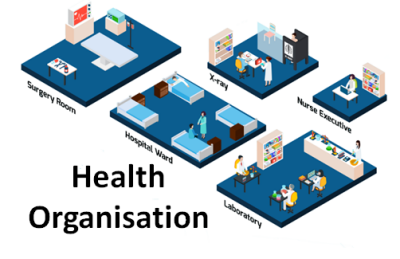
\includegraphics[width=\textwidth]{images/healthorganisation}}
\end{minipage}



%
% Now add in the appendices
%

\begin{appendices}
  %================================================================================
%       Safety Critical Systems Club - Data Safety Initiative Working Group
%================================================================================
%                       DDDD    SSSS  IIIII  W   W   GGGG
%                       D   D  S        I    W   W  G   
%                       D   D   SSS     I    W W W  G  GG
%                       D   D      S    I    WW WW  G   G
%                       DDDD   SSSS   IIIII  W   W   GGG
%================================================================================
%               Data Safety Guidance Document - LaTeX Source File
%================================================================================
%
% Description:
%   Activities and Tailoring section.
%
%================================================================================
\section{Linking Principles and Objectives (Informative)} \label{bkm:principlesobjectives}

\dsiwgSectionQuote
  {I'm a bit of a freak for evidence-based analysis. I strongly believe in data.}
  {Gus O'Donnell}


\subsection{General}

The Data Safety Assurance Principles provide the underpinning philosophy for \gls{dsg}. Conversely, an implementation of the guidance would be based around the objectives. It is thus appropriate to consider how meeting the objectives results in the Principles being satisfied. To that end, each Principle is considered in turn in the following paragraphs.


\subsection{Principle 1}
\dsiwgTextBF{\dsiwgTextIT{\index{Safety Requirement!Data}Data Safety Requirements shall be defined to address the data contribution to system hazards.}}

This Principle asks that requirements be defined. Hence, it is related to the Objective that:

\begin{itemize}
	\item \textcolor{dsiwgAccentColour}{4-1} \index{Safety Requirement!Data}Data Safety Requirements SHALL be established and elaborated.
\end{itemize}

However, that relationship does not tell the full story. In particular, the Principle is focused at a system level, whereas the above Objective is most likely to apply at more detailed levels of design. The following two objectives provide a system-level perspective on risks (from which specific requirements are developed) and hence both objectives directly support this Principle:

\begin{itemize}
	\item \textcolor{dsiwgAccentColour}{1-3} \index{Artefact, Data}\Glspl{data artefact} SHALL be identified.
	\item \textcolor{dsiwgAccentColour}{2-3} Risks SHALL be identified and linked to \index{Artefact, Data}\glspl{data artefact} and \index{Property!Data}\glspl{data property}.
\end{itemize}


\subsection{Principle 2}
\dsiwgTextBF{\dsiwgTextIT{The intent of \index{Safety Requirement!Data}Data Safety Requirements shall be maintained throughout requirements decomposition.}}

This Principle is based on standard systems engineering practices whereby a system is gradually developed at increasing levels of design detail. In order to cater for a wide range of systems, across a wide range of economic sectors, \gls{dsg} does not specifically require an explicit hierarchical decomposition of requirements. However, it does note that, if necessary, \index{Artefact, Data}\glspl{data artefact}s may be defined at a number of levels of increasing detail. Hence, the following two objectives are related to Principle 2:

\begin{itemize}
	\item \textcolor{dsiwgAccentColour}{1-3} \index{Artefact, Data}\Glspl{data artefact} SHALL be identified.
	\item \textcolor{dsiwgAccentColour}{2-3} Risks SHALL be identified and linked to \index{Artefact, Data}\glspl{data artefact} and \index{Property!Data}\glspl{data property}.
\end{itemize}

At a more fundamental level, this Principle is concerned with translating from high-level requirements to something that can be implemented. \Glspl{dsal} are a key element of this translation. As such, the following three objectives are also relevant:

\begin{itemize}
	\item \textcolor{dsiwgAccentColour}{3-1} \index{Assurance Level!Data}\Glspl{dsal} SHALL be established.
	\item \textcolor{dsiwgAccentColour}{3-2} \index{Assurance Level!Data}\Glspl{dsal} SHALL be justified.
	\item \textcolor{dsiwgAccentColour}{3-3} \index{Assurance Level!Data}\Glspl{dsal} SHALL be incorporated into system safety activities.
\end{itemize}

Note that the third of these objectives could also provide a direct link to hierarchical decomposition, if that activity is part of the system safety activities conducted by the organization implementing \gls{dsg}.

As noted earlier, this Principle is about identifying low-level design descriptions that, firstly, satisfy the intent of the high-level requirements and, secondly, are described in sufficient detail to allow them to be implemented (and for this implementation to be verified). From the perspective of \gls{dsg} these low-level items are \index{Safety Requirement!Data}Data Safety Requirements. Consequently, the following Objective also supports this Principle:

\begin{itemize}
	\item \textcolor{dsiwgAccentColour}{4-1} \index{Safety Requirement!Data}Data Safety Requirements SHALL be established and elaborated.
\end{itemize}


\subsection{Principle 3}
\dsiwgTextBF{\dsiwgTextIT{\index{Safety Requirement!Data}Data Safety Requirements shall be satisfied.}}

This Principle is straightforward. It involves implementing the low-level design descriptions and verifying these implementations. As such, it is directly supported by the following objectives:

\begin{itemize}
	\item \textcolor{dsiwgAccentColour}{4-2} Methods used to provide Data Safety assurance SHALL be defined and implemented.
	\item \textcolor{dsiwgAccentColour}{4-3} Compliance with \index{Safety Requirement!Data}Data Safety Requirements SHALL be demonstrated.	
\end{itemize}


\subsection{Principle 4}
\dsiwgTextBF{\dsiwgTextIT{Hazardous system behaviour arising from the system's use of data shall be identified and mitigated\index{Mitigation}.}}

From one perspective this Principle is about looking bottom-up to determine whether the detailed design decisions have introduced any new system-level risks. A \gls{hazop} is one way this can be achieved. Similarly, a \gls{hazop} is one of several techniques that \gls{dsg} suggests can be used to achieve the following objectives, which consequently may support Principle 4:

\begin{itemize}
	\item \textcolor{dsiwgAccentColour}{2-2} Unintended behaviour resulting from data SHALL be identified and analysed.
	\item \textcolor{dsiwgAccentColour}{2-3} Risks SHALL be identified and linked to \index{Artefact, Data}\glspl{data artefact} and \index{Property!Data}\glspl{data property}.
\end{itemize}

More generally, identifying potential new system-level hazards introduced by detailed design decisions involves looking at the system from a variety of perspectives. One perspective that is useful is provided by historical accidents and incidents; another useful perspective is provided by top-level generic data-related issues, distilled from experience across a wide range of systems and activities. Hence, the following Objective also supports Principle 4:

\begin{itemize}
	\item \textcolor{dsiwgAccentColour}{2-1} Historical data-related accidents and incidents SHALL be reviewed.
\end{itemize}

In addition, understanding the system context and intended use, as well as perspectives provided by a suitably wide collection of \index{Stakeholder}Stakeholders can inform risk considerations. Likewise, potential issues can also be identified by considering the boundaries of the system. It follows that the following three objectives are also relevant to Principle 4:

\begin{itemize}
	\item \textcolor{dsiwgAccentColour}{1-1} System context and intended use SHALL be established.
	\item \textcolor{dsiwgAccentColour}{1-2} Key \index{Stakeholder}Stakeholders SHALL be identified.
	\item \textcolor{dsiwgAccentColour}{1-4} Interfaces\index{Interface!System} SHALL be defined and managed.
\end{itemize}


\subsection{Principle 4 + 1}
\dsiwgTextBF{\dsiwgTextIT{The confidence established in addressing the Data Safety Assurance Principles shall be commensurate to the contribution of data to system risk.}}

This Principle provides a means of balancing available effort against risk. From the perspective of \gls{dsg}, this is provided by \index{Assurance Level!Data}\glspl{dsal}. As such, this Principle is directly supported by the following three objectives:

\begin{itemize}
	\item \textcolor{dsiwgAccentColour}{3-1} \index{Assurance Level!Data}\Glspl{dsal} SHALL be established.
	\item \textcolor{dsiwgAccentColour}{3-2} \index{Assurance Level!Data}\Glspl{dsal} SHALL be justified.
	\item \textcolor{dsiwgAccentColour}{3-3} \index{Assurance Level!Data}\Glspl{dsal} SHALL be incorporated into system safety activities.
\end{itemize}


\subsection{Summary Table}

For ease of reference, \autoref{tab:PrinciplesObjectivesSummary} summarises links between the Principles and objectives; these are shown by an ``X'' in the relevant cell. For completeness, this table shows the phase associated with each group of objectives. 

Two things are apparent from this table. Firstly, each Principle is supported by at least two objectives. Secondly, with one exception, each Objective supports at least one Principle. The exception is the Objective that ``A \index{Safety Assessment!Data}\gls{safety assessment} SHALL be planned'', which acts as an overarching Objective to ensure there is sufficient resource to meet the other objectives. For this reason it is loosely associated with each Principle; this is shown by an ``o'' in relevant cells.

Having each Principle supported by at least two objectives, along with the descriptive text above, provides confidence that meeting the objectives will satisfy the Principles; equivalently, it provides confident that the collection of objectives is \dsiwgTextIT{sufficient} to satisfy the Principles. 

In addition, every Objective supporting at least one Principle (with the exception noted above) indicates that there is value in each Objective being included in \gls{dsg}. This observation is not quite enough to demonstrate that the collection of objectives is \dsiwgTextIT{necessary} to satisfy the Principles. However, given the small number of objectives and the apparent lack of overlap between them, it is sufficient to suggest the necessity of the objectives.

\begin{longtable}{|C{\dsiwgColumnWidth{0.5}}|C{\dsiwgColumnWidth{0.08}}|C{\dsiwgColumnWidth{0.08}}|C{\dsiwgColumnWidth{0.08}}|C{\dsiwgColumnWidth{0.08}}|C{\dsiwgColumnWidth{0.08}}|}
  \caption{Principles and Objectives: Summary Table}
  \label{tab:PrinciplesObjectivesSummary}
  \\\hline
  \TableHeadColour{} & \multicolumn{5}{c|}{\TableHeadColourCX{Principle}}\\\cline{2-6}
  \multirow{-2}*{\TableHeadColourCX{}} & \TableHeadColourCX{P1} & \TableHeadColourCX{P2} & \TableHeadColourCX{P3} & \TableHeadColourCX{P4} & \TableHeadColourCX{P4+1}\\\hline
  \endfirsthead
  \caption[]{Principles and Objectives: Summary Table (continued)}
  \\\hline
  \TableHeadColour{} & \multicolumn{5}{c|}{\TableHeadColourCX{Principle}}\\\cline{2-6}
  \multirow{-2}*{\TableHeadColourCX{}} & \TableHeadColourCX{P1} & \TableHeadColourCX{P2} & \TableHeadColourCX{P3} & \TableHeadColourCX{P4} & \TableHeadColourCX{P4+1}\\\hline
  \endhead
  \multicolumn{6}{r}{\sl Continued on next page}
  \endfoot
  \endlastfoot
  \multicolumn{6}{|c|}{\dsiwgTextBF{Establish Context}}\\ \hline
	1-1 System context and intended use SHALL be established. & & & & X & \\ \hline
	1-2 Key \index{Stakeholder}Stakeholders SHALL be identified. & & & & X & \\ \hline
	1-3 \Glspl{data artefact}\index{Artefact, Data} SHALL be identified. & X & X & & & \\ \hline
	1-4 Interfaces\index{Interface!System} SHALL be defined and managed. & & & & X & \\ \hline
	1-5 A \index{Safety Assessment!Data}\Gls{safety assessment} SHALL be planned. & o & o & o & o & o\\ \hline
  \multicolumn{6}{|c|}{\dsiwgTextBF{Identify Risks}}\\ \hline
	2-1 Historical data-related accidents and incidents SHALL be reviewed. & & & & X & \\ \hline
	2-2 Unintended behaviour resulting from data SHALL be identified and analysed. & & & & X & \\ \hline
	2-3 Risks SHALL be identified and linked to \glspl{data artefact}\index{Artefact, Data} and \index{Property!Data}\glspl{data property}. & X & X & & X & \\ \hline
  \multicolumn{6}{|c|}{\dsiwgTextBF{Analyse Risks}}\\ \hline
	3-1 \index{Assurance Level!Data}\Glspl{dsal} SHALL be established. & & X & & & X \\ \hline
	3-2 \index{Assurance Level!Data}\Glspl{dsal} SHALL be justified. & & X & & & X \\ \hline
	3-3 \index{Assurance Level!Data}\Glspl{dsal} SHALL be incorporated into system safety activities. & & X & & & X \\ \hline
  \multicolumn{6}{|c|}{\dsiwgTextBF{Evaluate and Treat Risks}}\\ \hline
	4-1 \index{Safety Requirement!Data}Data Safety Requirements SHALL be established and elaborated. & X & X & & & \\ \hline
	4-2 Methods used to provide Data Safety assurance SHALL be defined and implemented. & & & X & & \\ \hline
	4-3 Compliance with \index{Safety Requirement!Data}Data Safety Requirements SHALL be demonstrated.	& & & X & & \\ \hline
\end{longtable}

  %================================================================================
%       Safety Critical Systems Club - Data Safety Initiative Working Group
%================================================================================
%                       DDDD    SSSS  IIIII  W   W   GGGG
%                       D   D  S        I    W   W  G   
%                       D   D   SSS     I    W W W  G  GG
%                       D   D      S    I    WW WW  G   G
%                       DDDD   SSSS   IIIII  W   W   GGG
%================================================================================
%               Data Safety Guidance Document - LaTeX Source File
%================================================================================
%
% Description:
%   Organizational Data Risk Assessment section.
%
%================================================================================
\section{\ecapitalisewords{\glsentrylong{odr}} (Informative)} \label{bkm:assessment}

\dsiwgSectionQuote{Data is becoming the new raw material of business.}{Craig Mundie}

\dsiwgTextBF{Note: this questionnaire only provides an initial \gls{odr} assessment. Further work is required to establish the safety data risks in detail such as determining a \gls{dsal}\index{Assurance Level!Data} for relevant data sets.}

\begin{longtable*}{|L{\dsiwgColumnWidth{0.31}}|L{\dsiwgColumnWidth{0.23}}|L{\dsiwgColumnWidth{0.23}}|L{\dsiwgColumnWidth{0.23}}|}
  \hline\multicolumn{4}{|c|}{\TableHeadColour{\Gls{odr} Assessment Form}}\\\hline
  \endfirsthead
  \hline\multicolumn{4}{|c|}{\TableHeadColour{\gls{odr} Assessment Form}}\\\hline
  \endhead
  \endfoot\endlastfoot
  %
  %Large block of text explaining the form, spanning all four columns
  %Need to have each paragraph as its own table entry, along with blank entries
  %spanning all of the columns for space between the paragraphs.
  %
  \multicolumn{4}{|p{\dsiwgColumnWidth{1.0}}|}{\dsiwgTextIT{This form is used to determine the safety risk related to data for a particular organization and usage.}}\\
  \multicolumn{4}{|p{\dsiwgColumnWidth{1.0}}|}{}\\
  \multicolumn{4}{|p{\dsiwgColumnWidth{1.0}}|}{\dsiwgTextIT{This form must be completed from the perspective of \dsiwgTextBF{one} of the organizations involved; typically this will be the organization using the data or the contractor supplying the system that handles the data. This form needs to be completed for each instance / application / scope / risk profile and should consider a defined boundary for the analysis, e.g.\ the scope of supply for the contractor or the limit of the data user's operational responsibility. It may be useful for both contracting parties to complete the form from their respective positions to check the data risk responsibilities and apportionment.}}\\
  \multicolumn{4}{|p{\dsiwgColumnWidth{1.0}}|}{}\\
  \multicolumn{4}{|p{\dsiwgColumnWidth{1.0}}|}{\dsiwgTextIT{It is anticipated that this form will be used during early phases of a procurement or supply and also for changes to existing supplies. It can also be used to assess existing legacy scenarios.}}\\
  \multicolumn{4}{|p{\dsiwgColumnWidth{1.0}}|}{}\\
  \multicolumn{4}{|p{\dsiwgColumnWidth{1.0}}|}{\dsiwgTextIT{Answer the questions as they apply in the context of the scope of supply. Mark the \index{Response}response with the ``best'' fit for the given scenario. Note that not all elements have to be satisfied. For each \index{Response}response also add a brief justification for that particular selection as opposed to any other choice.}}\\
  \multicolumn{4}{|p{\dsiwgColumnWidth{1.0}}|}{}\\
  \multicolumn{4}{|p{\dsiwgColumnWidth{1.0}}|}{\dsiwgTextIT{If the answer to a question is completely unknown at this stage; it is suggested that the middle value or higher is chosen and an explanation added to the justification.}}\\
  \multicolumn{4}{|p{\dsiwgColumnWidth{1.0}}|}{}\\
  \multicolumn{4}{|p{\dsiwgColumnWidth{1.0}}|}{\dsiwgTextIT{When all the relevant questions have been answered and justified, add the scores together to give a final total and record the value in the appropriate field. Use this total to determine the final \gls{odr} level based on the stated ranges.}}\\
  \multicolumn{4}{|p{\dsiwgColumnWidth{1.0}}|}{}\\
  \multicolumn{4}{|p{\dsiwgColumnWidth{1.0}}|}{\dsiwgTextIT{The \gls{odr} level determined may be used to
      support process tailoring and to
      determine the management regime required to mitigate the risk associated with the data.}}\\
  \hline
  %
  %Now the details of the form
  %
  Data Scenario/Context Name: & \multicolumn{3}{l|}{}\\
  \hline
  Data Scenario/Context Description: & \multicolumn{3}{l|}{}\\
  \hline
  Scope/Data Boundary and Perspective: & \multicolumn{3}{l|}{}\\
  \hline
  Completed By: & & Date Completed: & \\
  \hline
  %
  %Finally the last instruction for this part of the form.
  %Again, a block of text spanning all four columns.
  %
  \multicolumn{4}{|p{\dsiwgColumnWidth{1.0}}|}{\dsiwgTextIT{Answer each question using the \index{Response}response that forms the best match for the particular scenario. Not all statements have to be satisfied and some judgement is required; it is expected that the majority of statements in the selected \index{Response}response can be satisfied with some interpretation. The use of multiple criteria in each question enables a smaller and manageable set of questions to be posed to provide a holistic view of the overall risk.}}\\
  \hline
\end{longtable*}

%================================================================================
%Now the actual question tables themselves
%================================================================================
\clearpage %Start these on a new page

%
%Question 1
%
\begin{longtable*}{|C{\dsiwgColumnWidth{0.05}}|L{\dsiwgColumnWidth{0.85}}|C{\dsiwgColumnWidth{0.05}}|C{\dsiwgColumnWidth{0.05}}|}
  \hline\multicolumn{4}{|c|}{\TableHeadColour{QUESTION 1 --- SEVERITY AND PROXIMITY}}\\\hline
  \endfirsthead
  \hline\multicolumn{4}{|c|}{\TableHeadColour{QUESTION 1 --- SEVERITY AND PROXIMITY}}\\\hline
  \endhead
  \endfoot\endlastfoot
  \multicolumn{4}{|p{\dsiwgColumnWidth{1.0}}|}{\dsiwgTextBF{How severe could an accident be that is related to the data? Could it be caused directly by the data?}}\\
  \multicolumn{4}{|p{\dsiwgColumnWidth{1.0}}|}{\dsiwgTextIT{This question considers the safety consequence, the proximity and contribution of the data to the accident sequence.}}\\
  \hline
  1a & All currently foreseen uses of the data could not contribute to an accident. The data is not relied upon for safe operation. Negligible environmental impact. & 1 & \dsiwgCheckBox \\
  \hline
  1b & A possible use of data could contribute to a minor accident, but only via lengthy and indirect routes. Could lead to minor injury or temporary discomfort for 1 or 2 people. Many other people/systems are involved in checking the data. Some aspects of safe operation rely very indirectly on the data. Minor environmental impact only via indirect routes. & 2 & \dsiwgCheckBox \\
  \hline
  1c & A use of the data could lead to a significant accident resulting in minor injuries affecting several people or one serious injury. Several other people/systems are involved in checking the data. There is a dependency on the data for safe operation. Environmental impact is possible. & 4 & \dsiwgCheckBox \\
  \hline
  1d & A likely use of the data could directly lead to a serious accident resulting in serious injuries affecting a number of people, or a single death. One human or independent check is involved for all data. There is major dependency on the data for safe operation. Major environmental impact is possible. & 8 & \dsiwgCheckBox \\
  \hline
  1e & An intended use of the data could lead to an accident resulting in death for several people. The accident could be caused by the data with little chance of anything else detecting and mitigating the data issues. The accident could affect the general public or cause catastrophic environmental impact. & 16 & \dsiwgCheckBox \\
  \hline
  \multicolumn{4}{|p{\dsiwgColumnWidth{1.0}}|}{\dsiwgTextBF{Justification:}}\\*
  \multicolumn{4}{|p{\dsiwgColumnWidth{1.0}}|}{}\\*
  \multicolumn{4}{|p{\dsiwgColumnWidth{1.0}}|}{}\\
  \hline
\end{longtable*}

%
%Question 2
%
\begin{longtable*}{|C{\dsiwgColumnWidth{0.05}}|L{\dsiwgColumnWidth{0.85}}|C{\dsiwgColumnWidth{0.05}}|C{\dsiwgColumnWidth{0.05}}|}
  \hline\multicolumn{4}{|c|}{\TableHeadColour{QUESTION 2 --- ORGANIZATIONAL AND SOCIETAL IMPACT}}\\\hline
  \endfirsthead
  \hline\multicolumn{4}{|c|}{\TableHeadColour{QUESTION 2 --- ORGANIZATIONAL AND SOCIETAL IMPACT}}\\\hline
  \endhead
  \endfoot\endlastfoot
  \multicolumn{4}{|p{\dsiwgColumnWidth{1.0}}|}{\dsiwgTextBF{What would be the impact on the organization, client or public if an accident occurred related to the data?}}\\
  \multicolumn{4}{|p{\dsiwgColumnWidth{1.0}}|}{\dsiwgTextIT{This question considers the tolerability within this industry sector and the general public. How much would it affect the organization or society? Would a claim be likely? Would it generate press interest? Would a formal investigation ensue?}}\\
  \hline
  2a & Little interest, accidents happen all the time in this sector; very high societal tolerability. Negligible chance of claims or investigations. No adverse publicity likely. & 1 & \dsiwgCheckBox \\
  \hline
  2b & Some concern from the client, but accidents happen occasionally; high societal tolerability. Small chance of claim against the organization. Local or specialist press interest. Minor investigation or audit. & 2 & \dsiwgCheckBox \\
  \hline
  2c & Public would be concerned, accidents are rare in this sector; some societal tolerability. Significant chance of claim against the organization. Regional press interest. Client inquiry or investigation likely. & 4 & \dsiwgCheckBox \\
  \hline
  2d & Public would be alarmed and consider the accident a result of poor practice; little societal tolerability. Claims very likely. National press or media coverage a possibility. Legal or independent inquiry may follow. & 8 & \dsiwgCheckBox \\
  \hline
  2e & Public would be outraged and consider such an accident unacceptable; almost no societal tolerability. Multiple claims/fines from regulators or courts are likely. International press or media coverage. Official and / or public enquiry possible. & 16 & \dsiwgCheckBox \\
  \hline
  \multicolumn{4}{|p{\dsiwgColumnWidth{1.0}}|}{\dsiwgTextBF{Justification:}}\\*
  \multicolumn{4}{|p{\dsiwgColumnWidth{1.0}}|}{}\\*
  \multicolumn{4}{|p{\dsiwgColumnWidth{1.0}}|}{}\\
  \hline
\end{longtable*}

%
%Question 3
%
\begin{longtable*}{|C{\dsiwgColumnWidth{0.05}}|L{\dsiwgColumnWidth{0.85}}|C{\dsiwgColumnWidth{0.05}}|C{\dsiwgColumnWidth{0.05}}|}
  \hline\multicolumn{4}{|c|}{\TableHeadColour{QUESTION 3 --- RESPONSIBILITY}}\\\hline
  \endfirsthead
  \hline\multicolumn{4}{|c|}{\TableHeadColour{QUESTION 3 --- RESPONSIBILITY}}\\\hline
  \endhead
  \endfoot\endlastfoot
  \multicolumn{4}{|p{\dsiwgColumnWidth{1.0}}|}{\dsiwgTextBF{How much responsibility does this organization have for data safety?}}\\
  \multicolumn{4}{|p{\dsiwgColumnWidth{1.0}}|}{\dsiwgTextIT{This question considers how much legal and other responsibility and ownership the organization has for data safety aspects within this scenario. What liabilities for consequential losses/3rd party claims does the organization have via the contract or other means? What is the scale of the organization's contribution to the overall scope?}}\\
  \hline
  3a & The organization is not responsible for any data safety aspects. No liabilities for accident claims related to the data lie with the organization. Client or other party has accepted full data safety responsibility. The organization is fully covered and indemnified by the client or a 3rd party. & 1 & \dsiwgCheckBox \\
  \hline
  3b & The organization is a small part of a large consortium. It has minimal liability for data safety via the contract. It is partly covered by explicit client or 3rd party protections. All safety data is managed by subcontractors, the organization only reviews and monitors. & 2 & \dsiwgCheckBox \\
  \hline
  3c & The organization is a significant part of the consortium team. It has some share of the data safety responsibility. Specific data safety liabilities to the client via the contract are mentioned. There are no indemnities in the organization's favour. All key safety data obligations are explicitly flowed down to subcontractors. & 4 & \dsiwgCheckBox \\
  \hline
  3d & The organization is prime for a small programme or has the bulk of the data safety responsibility within a team. Specific accident-related liabilities in the contract are significant. The organization provides some indemnities to others via the contract. Some significant data safety obligations are not flowed down to subcontractors. & 7 & \dsiwgCheckBox \\
  \hline
  3e & The organization is priming a major programme or has total data safety responsibility. Specific accident-related liabilities in the contract are large (or unlimited). The organization provides explicit indemnities in favour of the client/3rd parties for accidents. Safety data obligations have not been discussed or are not flowed down to subcontractors. & 12 & \dsiwgCheckBox \\
  \hline
  \multicolumn{4}{|p{\dsiwgColumnWidth{1.0}}|}{\dsiwgTextBF{Justification:}}\\*
  \multicolumn{4}{|p{\dsiwgColumnWidth{1.0}}|}{}\\*
  \multicolumn{4}{|p{\dsiwgColumnWidth{1.0}}|}{}\\
  \hline
\end{longtable*}

%
%Question 4
%
\begin{longtable*}{|C{\dsiwgColumnWidth{0.05}}|L{\dsiwgColumnWidth{0.85}}|C{\dsiwgColumnWidth{0.05}}|C{\dsiwgColumnWidth{0.05}}|}
  \hline\multicolumn{4}{|c|}{\TableHeadColour{QUESTION 4 --- LEGAL AND REGULATORY FRAMEWORK}}\\\hline
  \endfirsthead
  \hline\multicolumn{4}{|c|}{\TableHeadColour{QUESTION 4 --- LEGAL AND REGULATORY FRAMEWORK}}\\\hline
  \endhead
  \endfoot\endlastfoot
  \multicolumn{4}{|p{\dsiwgColumnWidth{1.0}}|}{\dsiwgTextBF{What legal and regulatory environment will this work be subject to?}}\\
  \multicolumn{4}{|p{\dsiwgColumnWidth{1.0}}|}{\dsiwgTextIT{This question considers the legal and regulatory obligations that this work will have to conform to. How well is the legal framework defined and understood? Is there an established standards culture? Is there a regulator and certification process?}}\\
  \hline
  4a & Well-understood and tested legal framework, one jurisdiction. Highly regulated sector with one overseeing body. Well-established industry guidelines and standards for safety data. Formal certification processes. & 1 & \dsiwgCheckBox \\
  \hline
  4b & Understood and established legal framework, a few related jurisdictions. Regulated sector, more than one overseeing body. Industry guidelines and standards for safety data. Some formal certification processes. & 2 & \dsiwgCheckBox \\
  \hline
  4c & Some understanding of legal position, several jurisdictions. Partially regulated sector, several possible overseeing bodies. Some industry guidelines and standards that refer to data. Informal certification processes. & 4 & \dsiwgCheckBox \\
  \hline
  4d & Complex, poorly defined legal position, multiple different jurisdictions. Largely unregulated sector with no established overseeing body. Some industry guidelines and standards that mention data. Some informal certification processes. & 6 & \dsiwgCheckBox \\
  \hline
  4e & Very complex, untested and unclear legal position, many diverse jurisdictions. Unregulated sector with no overseeing body. No industry guidelines or standards for data. No certification processes. & 10 & \dsiwgCheckBox \\
  \hline
  \multicolumn{4}{|p{\dsiwgColumnWidth{1.0}}|}{\dsiwgTextBF{Justification:}}\\*
  \multicolumn{4}{|p{\dsiwgColumnWidth{1.0}}|}{}\\*
  \multicolumn{4}{|p{\dsiwgColumnWidth{1.0}}|}{}\\
  \hline
\end{longtable*}

%
%Question 5
%
\begin{longtable*}{|C{\dsiwgColumnWidth{0.05}}|L{\dsiwgColumnWidth{0.85}}|C{\dsiwgColumnWidth{0.05}}|C{\dsiwgColumnWidth{0.05}}|}
  \hline\multicolumn{4}{|c|}{\TableHeadColour{QUESTION 5 --- ORGANIZATIONAL MATURITY}}\\\hline
  \endfirsthead
  \hline\multicolumn{4}{|c|}{\TableHeadColour{QUESTION 5 --- ORGANIZATIONAL MATURITY}}\\\hline
  \endhead
  \endfoot\endlastfoot
  \multicolumn{4}{|p{\dsiwgColumnWidth{1.0}}|}{\dsiwgTextBF{How mature is this organiZation regarding data safety?}}\\
  \multicolumn{4}{|p{\dsiwgColumnWidth{1.0}}|}{\dsiwgTextIT{This question considers the maturity of the organization in relation to awareness and management of the risks associated with safety data. Are staff trained, managed and resourced to enable proper handling of data safety risk?}}\\
  \hline
  5a & Explicit recognition of data as a source of safety risk. Formal and established processes and procedures in place for the identification and control of safety data. Staff trained and fully aware of safety data risks. Senior management fully aware and supportive of data safety management activities. Management of safety data risks fully supported and funded. & 1 & \dsiwgCheckBox \\
  \hline
  5b & Awareness of data as a source of safety risk. Informal processes and procedures in place for the identification and control of safety data. Staff awareness of safety data risks. Senior management awareness of data safety management issues. Good support and funding for management of safety data risks. & 2 & \dsiwgCheckBox \\
  \hline
  5c & Some awareness of data as a source of safety risk. Some ad-hoc processes and procedures in place for the identification and control of safety data. Some staff awareness of safety data risks. Some senior management awareness of data safety management issues. Some support or partial funding for management of safety data risks. & 4 & \dsiwgCheckBox \\
  \hline
  5d & Little awareness of data as a source of safety risk. Minimal processes or procedures in place for the identification and control of safety data. Little staff awareness of safety data risks. Little senior management awareness of data safety management issues. Little support or minimal funding for management of safety data risks. & 7 & \dsiwgCheckBox \\
  \hline
  5e & No recognition of data as a source of safety risk. No processes or procedures in place for the identification or control of safety data. No staff training or awareness of safety data risks. Senior management not aware or in denial of safety data risks. No support or funding for management of safety data risks. & 10 & \dsiwgCheckBox \\
  \hline
  \multicolumn{4}{|p{\dsiwgColumnWidth{1.0}}|}{\dsiwgTextBF{Justification:}}\\*
  \multicolumn{4}{|p{\dsiwgColumnWidth{1.0}}|}{}\\*
  \multicolumn{4}{|p{\dsiwgColumnWidth{1.0}}|}{}\\
  \hline
\end{longtable*}

%
%Question 6
%
\begin{longtable*}{|C{\dsiwgColumnWidth{0.05}}|L{\dsiwgColumnWidth{0.85}}|C{\dsiwgColumnWidth{0.05}}|C{\dsiwgColumnWidth{0.05}}|}
  \hline\multicolumn{4}{|c|}{\TableHeadColour{QUESTION 6 --- OWNERSHIP AND USAGE}}\\\hline
  \endfirsthead
  \hline\multicolumn{4}{|c|}{\TableHeadColour{QUESTION 6 --- OWNERSHIP AND USAGE}}\\\hline
  \endhead
  \endfoot\endlastfoot
  \multicolumn{4}{|p{\dsiwgColumnWidth{1.0}}|}{\dsiwgTextBF{How widely is the data used and who by?}}\\
  \multicolumn{4}{|p{\dsiwgColumnWidth{1.0}}|}{\dsiwgTextIT{This question considers how much usage and what type of users there are likely to be of the data. How complex is the data supply chain? In what geographies is it used? How many \index{Data!Owner}owners and interfaces\index{Interface!Organizational} are there?}}\\
  \hline
  6a & Minimal or infrequent usage. One \index{Data!Owner}\gls{data owner}, a specialist highly trained user group. Single organization or recipient usage only. & 1 & \dsiwgCheckBox \\
  \hline
  6b & A number of operational data users. Simple linear supply chain. More than one \index{Data!Owner}\glspl{data owner}. Specialist user or limited public access. Small-scale operation. No general web access. Few user organizations or recipients. & 2 & \dsiwgCheckBox \\
  \hline
  6c & Regional usage. Some public or mainstream usage. A few supply chains. A few \index{Data!Owner}\glspl{data owner}. Some web access. Several user organizations or recipients. & 4 & \dsiwgCheckBox \\
  \hline
  6d & National usage. Public or mainstream usage. Several supply chains. Several \index{Data!Owner}\glspl{data owner}. Web access. Some or varied user organizations or recipients. & 7 & \dsiwgCheckBox \\
  \hline
  6e & International usage. Extensive public or mainstream usage. Extensive web access. Many complex supply chains. Many and diverse \index{Data!Owner}\glspl{data owner}. Many and diverse user organizations or recipients. & 12 & \dsiwgCheckBox \\
  \hline
  \multicolumn{4}{|p{\dsiwgColumnWidth{1.0}}|}{\dsiwgTextBF{Justification:}}\\*
  \multicolumn{4}{|p{\dsiwgColumnWidth{1.0}}|}{}\\*
  \multicolumn{4}{|p{\dsiwgColumnWidth{1.0}}|}{}\\
  \hline
\end{longtable*}

%
%Question 7
%
\begin{longtable*}{|C{\dsiwgColumnWidth{0.05}}|L{\dsiwgColumnWidth{0.85}}|C{\dsiwgColumnWidth{0.05}}|C{\dsiwgColumnWidth{0.05}}|}
  \hline\multicolumn{4}{|c|}{\TableHeadColour{QUESTION 7 --- SIZE, COMPLEXITY AND NOVELTY}}\\\hline
  \endfirsthead
  \hline\multicolumn{4}{|c|}{\TableHeadColour{QUESTION 7 --- SIZE, COMPLEXITY AND NOVELTY}}\\\hline
  \endhead
  \endfoot\endlastfoot
  \multicolumn{4}{|p{\dsiwgColumnWidth{1.0}}|}{\dsiwgTextBF{What is the scale, sophistication and complexity of the data and its manipulation?}}\\
  \multicolumn{4}{|p{\dsiwgColumnWidth{1.0}}|}{\dsiwgTextIT{This question considers the nature of the data, its lifecycle and how easy it is to detect errors in the data.}}\\
  \hline
  7a & Simple data structures. Mature and established data storage and manipulation techniques and technologies. One or two interfaces\index{Interface!System}. No timeliness\index{Timeliness Property} aspects. No transformations. Data is easily verifiable. Data is easily traceable to original source. & 1 & \dsiwgCheckBox \\
  \hline
  7b & Varied data structures. Mainstream data storage and manipulation techniques and technologies. Several interfaces\index{Interface!System}. Few timeliness\index{Timeliness Property} aspects. Few data transformations. Data is verifiable. Data is traceable to original source. & 2 & \dsiwgCheckBox \\
  \hline
  7c & Complex with some unstructured data. Current data storage and manipulation techniques and technologies. Multiple interfaces\index{Interface!System}. Some timeliness\index{Timeliness Property} aspects. Some data transformations. Data is difficult to verify. Data is difficult to trace back to original source. & 4 & \dsiwgCheckBox \\
  \hline
  7d & Complex, varied or partially unstructured data. Novel storage and manipulation techniques and technologies. Multiple complex interfaces\index{Interface!System}. Time critical. Complex data transformations. Data is very difficult to verify. Data is very difficult to trace back to original source. & 7 & \dsiwgCheckBox \\
  \hline
  7e & Highly complex, varied or unstructured data. Highly novel storage and manipulation techniques and technologies. Many and complex, ill-defined or dynamic interfaces\index{Interface!System}. Highly time critical. Many and complex data transformations. Data is infeasible to verify. Data is impossible to trace back to original source. & 10 & \dsiwgCheckBox \\
  \hline
  \multicolumn{4}{|p{\dsiwgColumnWidth{1.0}}|}{\dsiwgTextBF{Justification:}}\\*
  \multicolumn{4}{|p{\dsiwgColumnWidth{1.0}}|}{}\\*
  \multicolumn{4}{|p{\dsiwgColumnWidth{1.0}}|}{}\\
  \hline
\end{longtable*}

%
%Question 8
%
\begin{longtable*}{|C{\dsiwgColumnWidth{0.05}}|L{\dsiwgColumnWidth{0.85}}|C{\dsiwgColumnWidth{0.05}}|C{\dsiwgColumnWidth{0.05}}|}
  \hline\multicolumn{4}{|c|}{\TableHeadColour{QUESTION 8 --- BOUNDARIES AND INTERFACES}}\\\hline
  \endfirsthead
  \hline\multicolumn{4}{|c|}{\TableHeadColour{QUESTION 8 --- BOUNDARIES AND INTERFACES}}\\\hline
  \endhead
  \endfoot\endlastfoot
  \multicolumn{4}{|p{\dsiwgColumnWidth{1.0}}|}{\dsiwgTextBF{How well defined and understood are the boundaries and interfaces\index{Interface!System} for this data scenario?}}\\
  \multicolumn{4}{|p{\dsiwgColumnWidth{1.0}}|}{\dsiwgTextIT{This question considers the number, complexity and definition status of the boundaries and interfaces\index{Interface!System} where data is exchanged. How well understood are the boundaries and interfaces\index{Interface!System}? Are standard formats and protocols used? Is data exchange time critical? Are all assumptions and ambiguities relating to the data exchange resolved?}}\\
  \hline
  8a & One well-understood boundary and few, well-defined interfaces\index{Interface!System}. Standard interface formats and protocols. No timeliness\index{Timeliness Property} aspects to data exchange. No remaining ambiguities, TBCs or TBDs. No assumptions. & 1 & \dsiwgCheckBox \\
  \hline
  8b & A few, understood boundaries and several defined interfaces\index{Interface!System}. Mainly standard interface formats and protocols. Few timeliness\index{Timeliness Property} aspects to data exchange. Few areas of ambiguity, few TBCs and TBDs. Few assumptions. & 2 & \dsiwgCheckBox \\
  \hline
  8c & Several, established boundaries, some defined, some undefined and some ambiguous interfaces\index{Interface!System}. Mixture of standard and non-standard interface formats and protocols. Some timely data exchanges. Some areas of ambiguity, some TBCs and TBDs. Some assumptions. & 4 & \dsiwgCheckBox \\
  \hline
  8d & Many, poorly understood boundaries, many undefined or ambiguous interfaces\index{Interface!System}. Mostly non-standard interface formats and protocols. Time sensitive data exchange. Many areas of ambiguity, many TBCs and TBDs. Many assumptions. & 6 & \dsiwgCheckBox \\
  \hline
  8e & A large number of unclear boundaries; a large number of unknown and undefined interfaces\index{Interface!System}. Completely non-standard, complex interface formats and protocols. Real-time data exchange. Large areas of ambiguity, a large number of TBCs and TBDs. A large number of assumptions. & 10 & \dsiwgCheckBox \\
  \hline
  \multicolumn{4}{|p{\dsiwgColumnWidth{1.0}}|}{\dsiwgTextBF{Justification:}}\\*
  \multicolumn{4}{|p{\dsiwgColumnWidth{1.0}}|}{}\\*
  \multicolumn{4}{|p{\dsiwgColumnWidth{1.0}}|}{}\\
  \hline
\end{longtable*}

%
%ODR Level Table
%
\begin{longtable*}{|L{\dsiwgColumnWidth{0.75}}|C{\dsiwgColumnWidth{0.25}}|}
  \hline\multicolumn{2}{|c|}{\TableHeadColour{\GLStext{odr} LEVEL}}\\\hline
  \endfirsthead
  \hline\multicolumn{2}{|c|}{\TableHeadColour{\GLStext{odr} LEVEL}}\\\hline
  \endhead
  \endfoot\endlastfoot
  \multicolumn{2}{|p{\dsiwgColumnWidth{1.0}}|}{\dsiwgTextBF{Record the total score and use it to determine the \gls{odr} level based on the ranges given below. \underline{If the first three questions' scores sum up to 6 or less then disregard the scores for the remaining} \underline{questions.}}}\\
  \hline
  Score 14 or less & ODR0 \\
  \hline
  Score 15 to 21 & ODR1 \\
  \hline
  Score 22 to 37 & ODR2 \\
  \hline
  Score 38 to 47 & ODR3 \\
  \hline
  Score 48 and above & ODR4 \\
  \hline
  \dsiwgTextBF{Total Score for this scenario/context:} & \\
  \hline
  \dsiwgTextBF{\gls{odr} Level for this scenario/context:} & \\
  \hline
\end{longtable*}

  %================================================================================
%       Safety Critical Systems Club - Data Safety Initiative Working Group
%================================================================================
%                       DDDD    SSSS  IIIII  W   W   GGGG
%                       D   D  S        I    W   W  G   
%                       D   D   SSS     I    W W W  G  GG
%                       D   D      S    I    WW WW  G   G
%                       DDDD   SSSS   IIIII  W   W   GGG
%================================================================================
%               Data Safety Guidance Document - LaTeX Source File
%================================================================================
%
% Description:
%   Data Safety Culture Questionnaire section.
%
%================================================================================
\section{Data Safety Culture Questionnaire (Informative)} \label{bkm:culture}

\dsiwgSectionQuote{Data is the fabric of the modern world: just like we walk down pavements, so we trace routes through data and build knowledge and products out of it.}{Ben Goldacre}

This form helps an organization appreciate the data safety culture. It can be applied at various levels, including at the project level and at the organizational level.

\begin{longtable*}{|L{\dsiwgColumnWidth{0.25}}|L{\dsiwgColumnWidth{0.25}}|L{\dsiwgColumnWidth{0.25}}|L{\dsiwgColumnWidth{0.25}}|}
  \hline\multicolumn{4}{|c|}{\TableHeadColour{Data Safety Culture Questionnaire Form}}\\\hline
  \endfirsthead
  \hline\multicolumn{4}{|c|}{\TableHeadColour{Data Safety Culture Questionnaire Form}}\\\hline
  \endhead
  \endfoot\endlastfoot
  %
  %Large block of text explaining the form, spanning all four columns
  %Need to have each paragraph as its own table entry, along with blank entries
  %spanning all of the columns for space between the paragraphs.
  %
  \multicolumn{4}{|p{\dsiwgColumnWidth{1.0}}|}{\dsiwgTextIT{This form is used to assess the safety culture related to data for a particular programme.}}\\
%  \multicolumn{4}{|p{\dsiwgColumnWidth{1.0}}|}{}\\
  \multicolumn{4}{|p{\dsiwgColumnWidth{1.0}}|}{\dsiwgTextBF{You play a key role in protecting the organization from data safety risks and your views are important. This self-assessment survey is designed to assess our current level of data safety culture within the programme. The output can help us to improve our safety position.}}\\
%  \multicolumn{4}{|p{\dsiwgColumnWidth{1.0}}|}{}\\
  \multicolumn{4}{|p{\dsiwgColumnWidth{1.0}}|}{Please tick the box which reflects your view and answer as honestly as possible. Space is provided for explanatory comments. Your response will only be of value if it reflects what you actually believe is the case, rather than what you believe should happen.}\\
%  \multicolumn{4}{|p{\dsiwgColumnWidth{1.0}}|}{}\\
  \multicolumn{4}{|p{\dsiwgColumnWidth{1.0}}|}{If you would like to remain anonymous please print and send this form by post.}\\
%  \multicolumn{4}{|p{\dsiwgColumnWidth{1.0}}|}{}\\
  \multicolumn{4}{|p{\dsiwgColumnWidth{1.0}}|}{The survey should take no longer than 10 minutes. It is anticipated that this form will be used on a regular basis (e.g.\ annually).}\\
  \hline
  %
  %Now the details of the form
  %
  Programme Name: & \multicolumn{3}{l|}{}\\
  \hline
  Data Scenario / Context Description: & \multicolumn{3}{l|}{}\\
  \hline
  Completed By: & & Date Completed: & \\
  \hline
  %
  %Finally the last instruction for this part of the form.
  %Again, a block of text spanning all four columns.
  %
  \multicolumn{4}{|c|}{\dsiwgTextBF{\dsiwgTextIT{Answer each question as you see it - there is no right answer!}}}\\
  \hline
\end{longtable*}

%================================================================================
%Now the actual question tables themselves
%================================================================================

%
%Question 1
%
\begin{longtable*}{|C{\dsiwgColumnWidth{0.05}}|L{\dsiwgColumnWidth{0.38}}|C{\dsiwgColumnWidth{0.08}}|C{\dsiwgColumnWidth{0.11}}%
                  |C{\dsiwgColumnWidth{0.11}}|C{\dsiwgColumnWidth{0.09}}|C{\dsiwgColumnWidth{0.08}}|C{\dsiwgColumnWidth{0.10}}|}
  \hline\multicolumn{8}{|c|}{\TableHeadColour{QUESTION 1 --- MY VIEW OF OUR SUPPLY}}\\\hline
  \multicolumn{2}{|l|}{} & Don't Know & Strongly Disagree & Disagree & Maybe & Agree & Strongly Agree\\\hline
  \endfirsthead
  \hline\multicolumn{8}{|c|}{\TableHeadColour{QUESTION 1 --- MY VIEW OF OUR SUPPLY}}\\\hline
  \multicolumn{2}{|l|}{} & Don't Know & Strongly Disagree & Disagree & Maybe & Agree & Strongly Agree\\\hline
  \endhead
  \endfoot\endlastfoot
  1a & I see data as an important factor in the safety of my programme. & \dsiwgCheckBox & \dsiwgCheckBox & \dsiwgCheckBox & \dsiwgCheckBox & \dsiwgCheckBox & \dsiwgCheckBox \\
  \hline
  1b & I am familiar with the safety aspects of our data. & \dsiwgCheckBox & \dsiwgCheckBox & \dsiwgCheckBox & \dsiwgCheckBox & \dsiwgCheckBox & \dsiwgCheckBox \\
  \hline
  1c & I understand how data in our solution can contribute to an accident. & \dsiwgCheckBox & \dsiwgCheckBox & \dsiwgCheckBox & \dsiwgCheckBox & \dsiwgCheckBox & \dsiwgCheckBox \\
  \hline
  1d & I think we could be blamed if there were an accident due to our data. & \dsiwgCheckBox & \dsiwgCheckBox & \dsiwgCheckBox & \dsiwgCheckBox & \dsiwgCheckBox & \dsiwgCheckBox \\
  \hline
  \multicolumn{8}{|p{\dsiwgColumnWidth{1.0}}|}{\dsiwgTextBF{Comments:}}\\*
  \multicolumn{8}{|p{\dsiwgColumnWidth{1.0}}|}{}\\*
  \multicolumn{8}{|p{\dsiwgColumnWidth{1.0}}|}{}\\
  \hline
\end{longtable*}

%
%Question 2
%
\begin{longtable*}{|C{\dsiwgColumnWidth{0.05}}|L{\dsiwgColumnWidth{0.38}}|C{\dsiwgColumnWidth{0.08}}|C{\dsiwgColumnWidth{0.11}}%
                  |C{\dsiwgColumnWidth{0.11}}|C{\dsiwgColumnWidth{0.09}}|C{\dsiwgColumnWidth{0.08}}|C{\dsiwgColumnWidth{0.10}}|}
  \hline\multicolumn{8}{|c|}{\TableHeadColour{QUESTION 2 --- WHAT WE'RE DOING}}\\\hline
  \multicolumn{2}{|l|}{} & Don't Know & Strongly Disagree & Disagree & Maybe & Agree & Strongly Agree\\\hline
  \endfirsthead
  \hline\multicolumn{8}{|c|}{\TableHeadColour{QUESTION 2 --- WHAT WE'RE DOING}}\\\hline
  \multicolumn{2}{|l|}{} & Don't Know & Strongly Disagree & Disagree & Maybe & Agree & Strongly Agree\\\hline
  \endhead
  \endfoot\endlastfoot
  2a & I think that the programme is aware of data safety risks. & \dsiwgCheckBox & \dsiwgCheckBox & \dsiwgCheckBox & \dsiwgCheckBox & \dsiwgCheckBox & \dsiwgCheckBox \\
  \hline
  2b & I believe we need to implement measures to manage data safety risks. & \dsiwgCheckBox & \dsiwgCheckBox & \dsiwgCheckBox & \dsiwgCheckBox & \dsiwgCheckBox & \dsiwgCheckBox \\
  \hline
  2c & I think that the programme meets its obligations (e.g.\ has a Data Management Plan in place and a role with specific responsibilities in this area). & \dsiwgCheckBox & \dsiwgCheckBox & \dsiwgCheckBox & \dsiwgCheckBox & \dsiwgCheckBox & \dsiwgCheckBox \\
  \hline
  \multicolumn{8}{|p{\dsiwgColumnWidth{1.0}}|}{\dsiwgTextBF{Comments:}}\\*
  \multicolumn{8}{|p{\dsiwgColumnWidth{1.0}}|}{}\\*
  \multicolumn{8}{|p{\dsiwgColumnWidth{1.0}}|}{}\\
  \hline
\end{longtable*}

%
%Question 3
%
\begin{longtable*}{|C{\dsiwgColumnWidth{0.05}}|L{\dsiwgColumnWidth{0.38}}|C{\dsiwgColumnWidth{0.08}}|C{\dsiwgColumnWidth{0.11}}%
                  |C{\dsiwgColumnWidth{0.11}}|C{\dsiwgColumnWidth{0.09}}|C{\dsiwgColumnWidth{0.08}}|C{\dsiwgColumnWidth{0.10}}|}
  \hline\multicolumn{8}{|c|}{\TableHeadColour{QUESTION 3 --- MY ROLE}}\\\hline
  \multicolumn{2}{|l|}{} & Don't Know & Strongly Disagree & Disagree & Maybe & Agree & Strongly Agree\\\hline
  \endfirsthead
  \hline\multicolumn{8}{|c|}{\TableHeadColour{QUESTION 3 --- MY ROLE}}\\\hline
  \multicolumn{2}{|l|}{} & Don't Know & Strongly Disagree & Disagree & Maybe & Agree & Strongly Agree\\\hline
  \endhead
  \endfoot\endlastfoot
  3a & I know my role relates to the management of data and associated safety risks. & \dsiwgCheckBox & \dsiwgCheckBox & \dsiwgCheckBox & \dsiwgCheckBox & \dsiwgCheckBox & \dsiwgCheckBox \\
  \hline
  3b & If I had a safety concern about our data I would report it. & \dsiwgCheckBox & \dsiwgCheckBox & \dsiwgCheckBox & \dsiwgCheckBox & \dsiwgCheckBox & \dsiwgCheckBox \\
  \hline
  3c & I know who the data safety representative is on my programme. & \dsiwgCheckBox & \dsiwgCheckBox & \dsiwgCheckBox & \dsiwgCheckBox & \dsiwgCheckBox & \dsiwgCheckBox \\
  \hline
  3d & I have received adequate training regarding data safety for my role. & \dsiwgCheckBox & \dsiwgCheckBox & \dsiwgCheckBox & \dsiwgCheckBox & \dsiwgCheckBox & \dsiwgCheckBox \\
  \hline
  3e & I feel supported in dealing with data safety risks. & \dsiwgCheckBox & \dsiwgCheckBox & \dsiwgCheckBox & \dsiwgCheckBox & \dsiwgCheckBox & \dsiwgCheckBox \\
  \hline
  3f & I have adequate time to address any data safety issues. & \dsiwgCheckBox & \dsiwgCheckBox & \dsiwgCheckBox & \dsiwgCheckBox & \dsiwgCheckBox & \dsiwgCheckBox \\
  \hline
  \multicolumn{8}{|p{\dsiwgColumnWidth{1.0}}|}{\dsiwgTextBF{Comments:}}\\*
  \multicolumn{8}{|p{\dsiwgColumnWidth{1.0}}|}{}\\*
  \multicolumn{8}{|p{\dsiwgColumnWidth{1.0}}|}{}\\
  \hline
\end{longtable*}

  %================================================================================
%       Safety Critical Systems Club - Data Safety Initiative Working Group
%================================================================================
%                       DDDD    SSSS  IIIII  W   W   GGGG
%                       D   D  S        I    W   W  G   
%                       D   D   SSS     I    W W W  G  GG
%                       D   D      S    I    WW WW  G   G
%                       DDDD   SSSS   IIIII  W   W   GGG
%================================================================================
%               Data Safety Guidance Document - LaTeX Source File
%================================================================================
%
% Description:
%   Supplier Data Maturity section.
%
%================================================================================
\section{Supplier Data Maturity (Informative)} \label{bkm:maturity}

\dsiwgSectionQuote{The most valuable thing you can have as a leader is clear data.}{Ruth Porat}

This questionnaire may be used for two purposes:
\begin{enumerate}
  \item To support a procurement process - distributed by an organization looking for a company that can handle safety-critical development, because the system they require to be developed is known to have safety-critical requirements
  \item Internal audits - used internally by a company developing systems with safety-related data which needs to assure itself of its capability to fulfil customer needs.
\end{enumerate}

\dsiwgTextBF{Organization}
\begin{enumerate}
  \item For each software development involving data, is there a designated data safety manager?
  \item If so, does the data safety manager report directly to the project manager?
  \item Are the management reporting channels for data assurance and software development separate?
  \item Is data subject to a formal configuration control process? 
  \item Is data engineering represented on the system design team?
  \item Is data engineering process improvement part of the company quality systems?
\end{enumerate}

\dsiwgTextBF{Resources, Personnel and Training}
\begin{enumerate}
  \item Are personnel specified as responsible for data safety as a separate role from software and system design and development?
  \item Is there a required training programme for data specialists?
  \item Is training on data safety issues part of the training for managers or management teams?
  \item Is there a formal training programme for data safety design and review leaders
\end{enumerate}

\dsiwgTextBF{Data Issues Growth Management}
\begin{enumerate}
  \item Is a mechanism employed for maintaining awareness of the state of the art in data safety technology?
  \item Is a mechanism employed for comparing the company approach to data safety with external processes for data safety practised elsewhere in the industry?
  \item Is a mechanism used for introducing new technologies and processes into system development?
  \item Is a mechanism in place for identifying and replacing obsolescent processes related to data safety?
\end{enumerate}

\clearpage% Move heading onto next page (doesn't align with 3.2, but corrects layout error)
\dsiwgTextBF{Documented Standards and Procedures}
\begin{enumerate}
  \item Describe any formal procedures adopted at each periodic management review to assess the status of data related to the system.
  \item Describe the methods used for ensuring that the data development team understands each data requirement.
  \item Is a data risk assessment method used for assessing the use of existing data in new applications?
  \item Are data test cases developed formally with a company standard?
  \item Is there a document which describes how the customer is to be consulted over data issues?
  \item Is particular care taken to capture requirements, design, review and test data for user interfaces\index{Interface!User}?
  \item Is there a data risk monitoring and tracking to closure procedure practised?
\end{enumerate}

\dsiwgTextBF{Process Metrics}
\begin{enumerate}
  \item Are statistics of failures due to data errors during development kept to feedback and learn from in future development?
  \item Are data issue action items tracked to closure and reports maintained of causes?
  \item Is configuration data separately developed from everyday operational data?
  \item Is data test coverage measured and recorded?
  \item Are all states, from which configuration data will be required, tested, (including emergency reboot), and results recorded?
  \item Are analyses of errors due to data conducted to determine their process related causes?
  \item Are the process causes reviewed and changes to processes implemented where appropriate?
\end{enumerate}

\dsiwgTextBF{Process Control}
\begin{enumerate}
  \item Is regression testing routinely performed when errors are discovered?
  \item Is the adequacy of regression testing subject to an assurance process to ensure new errors are not introduced?
  \item Is a mechanism used for identifying and resolving system engineering issues that affect data?
  \item Is a mechanism used for ensuring traceability between the data requirements and the top-level design?
  \item Is the importance of data in the system engineering process reviewed to maintain processes at an adequate level to cope with the expanding role of data in the Internet of Things? 
\end{enumerate}

  %================================================================================
%       Safety Critical Systems Club - Data Safety Initiative Working Group
%================================================================================
%                       DDDD    SSSS  IIIII  W   W   GGGG
%                       D   D  S        I    W   W  G   
%                       D   D   SSS     I    W W W  G  GG
%                       D   D      S    I    WW WW  G   G
%                       DDDD   SSSS   IIIII  W   W   GGG
%================================================================================
%               Data Safety Guidance Document - LaTeX Source File
%================================================================================
%
% Description:
%   Data Categories section.
%
%================================================================================
\section{Data Categories -- Detail (Informative)\index{Category!Data|textbf}} \label{bkm:categories}

\dsiwgSectionQuote{It's difficult to imagine the power that you're going to have when so many different sorts of data are available}{Tim Berners-Lee}

\autoref{tab:Categories} provides additional \gls{information}, in the form of explanations and lists of typical containers, for the identified Data Categories.

\begin{longtable}{|C{\dsiwgColumnWidth{0.06}}|L{\dsiwgColumnWidth{0.17}}|L{\dsiwgColumnWidth{0.17}}|L{\dsiwgColumnWidth{0.38}}|L{\dsiwgColumnWidth{0.22}}|}
  \caption{Categories of Safety-related Data: Detailed Definitions}
  \label{tab:Categories}
  \\\hline\TableHeadColourC{No.} & \TableHeadColour{Category} & \TableHeadColour{Description} & \TableHeadColour{Explanation} & \TableHeadColour{Typical containers}\\\hline
  \endfirsthead
  \caption[]{Categories of Safety-related Data: Detailed Definitions (continued)}
  \\\hline\TableHeadColourC{No.} & \TableHeadColour{Category} & \TableHeadColour{Description} & \TableHeadColour{Explanation} & \TableHeadColour{Typical containers}\\\hline
  \endhead
  \multicolumn{5}{r}{\sl Continued on next page}
  \endfoot\endlastfoot
  \hline
  \multicolumn{5}{|c|}{\dsiwgTextBF{Context}}\\
  \hline
  1 & Predictive\index{Predictive Data|textbf} & Data used to model or predict behaviours and performance & Data for studies, models, prototypes, initial risk assessments, etc.  This is the data produced during the initial concept phase which subsequently flows into further development phases. & Prototype results, evaluations, analyses\\
  \hline
  2 & Scope, Assumption and Context\index{Scope, Assumption and Context Data|textbf} & Data used to frame the development, operations or provide context & Restrictions, risk criteria, usage scenarios, etc.\ explaining how the system will be used and any limitations of use. & Concepts of operation, Safety Case Report Part~1 \\
  \hline
  3 & Requirements\index{Requirement Data|textbf} & Data used to specify what the system has to do & Data encompassing requirements, specifications, internal interface\index{Interface!System} or control definitions, data formats, etc. & Formal specifications, interface control documents\index{Interface!Control Document}, user requirements documents, Safety Case Report Part~1\\
  \hline
  4 & Interface\index{Interface Data|textbf} & Data used to enable interfaces between this system and other systems:  for operations, initialisation or export from the system & Data that exists to enable exchange between this system and other external systems. Covers start-of-life operations (data import or migration), end-of-life operations and ongoing operational exchange of data between systems. & Protocols, schemas, interface control documents\index{Interface!Control Document}, transition plans, Extract-Transform-Load tool specifications, cleansing and filtering rules\\
  \hline
  5 & Reference or Lookup\index{Reference or Lookup Data|textbf} & Data used across multiple systems with generic usage & Data comprising generic reference \gls{information} sets used by multiple systems (i.e., not produced solely for this system). Typically updated infrequently, and not specific to this system. & Dictionaries, materials \gls{information}, sector data reference sets, encyclopedias\\
  \hline
  \pagebreak[4]%4 chosen as an experiment, as 1-3 didn't work. We don't want the next line at the bottom of a page
  \multicolumn{5}{|c|}{\dsiwgTextBF{Implementation}}\\
  \hline
  6 & Design and Development\index{Design and Development Data|textbf} & Data produced during development  and implementation & Data encompassing the design and development process artefacts: everything from design models and schemas to document review records.  It also includes test documents (specification and results) but not the test data itself. & Design documents, review records, hardware, software, test scripts, code inspection reports, Safety Case Report Part~2\\
  \hline
  7 & Software\index{Software Data|textbf} & Data that is compiled (or interpreted) and executed to achieve the desired system behaviour & From some perspectives it is helpful to consider software (e.g., source code) as another category of data. & Text files, configuration management systems\\
  \hline
  8 & Verification\index{Verification Data|textbf} & Data used to test and analyse the system & Data comprising the test values and test data sets used to verify the system. It might include real data, modified real data or synthetic data. It includes data used to drive stubs, and any data files used by simulators or emulators. & Test data sets, stub data, emulator and simulator files\\
  \hline
  \multicolumn{5}{|c|}{\dsiwgTextBF{Configuration}}\\
  \hline
	9 & \Gls{ml}\index{Machine Learning Data|textbf} & Data used to train the system to enable it to learn from the characteristics of the data & Data used to train, set up or adapt the system for a particular purpose or configuration. Might be subsets of real data or synthetically produced. Might have to include or exclude corner cases. & Images for pattern recognition analysis \\
	\hline
  10 & Infrastructure\index{Infrastructure Data|textbf} & Data used to configure, tailor or instantiate the system itself & Data used to set up and configure the system for a particular installation, product configuration, or network environment. & Network configuration files, initialisation files, hardware pin settings, network addresses, passwords \\
  \hline
  11 & Behavioural\index{Behavioural Data|textbf} & Data used to change the functionality of the system & Data to enable / disable or configure functions or behaviour of the system. & \gls{xml} configuration files, \gls{csv} data, schemas \\
  \hline
  12 & Adaptation\index{Adaptation Data|textbf} & Data used to configure to a particular site & Data used to tailor or calibrate a system to a particular physical site or environment, incorporating physical or environmental conditions. & Configuration files \\
  \hline
    \pagebreak[4]%4 chosen as an experiment, as 1-3 didn't work. We don't want the next line at the bottom of a page
\multicolumn{5}{|c|}{\dsiwgTextBF{Capability}}\\
  \hline
  13 &  Staffing\index{Staffing Data|textbf} & Data related to staff training, competency, certification and permits & Data which allows staff to perform a function within the wider context of the safety-related system. This might include training records, competency assessments, permits to work, etc. & Human Resources records, training certificates, card systems\\
  \hline
  \multicolumn{5}{|c|}{\dsiwgTextBF{The Built System}}\\
  \hline
  14 & Asset\index{Asset Data|textbf} & Data about the installed or deployed system and its parts, including maintenance data & Data related to location, condition and maintenance requirements of the system under consideration. This might cover hardware, software and data. & Inventory, asset and maintenance \gls{database} systems\\
  \hline
  15 & Performance\index{Performance Data|textbf} & Data collected or produced about the system during trials, pre-operational phases and live operations & Data produced by and about the system during introduction to service and live service itself. Includes fault data and diagnostic data. This might be the results of various phases of introduction and might include trend analysis to look for long-term problems. & Field data, Support calls, bug reports, non-compliance reports, \gls{dracas} data\\
  \hline
  16 & Release\index{Release Data|textbf} & Data used to ensure safe operations per release instance & Explanation of particular features or limitations of a release or instance. Might include specific time-limited workarounds and caveats for a release. & Release notes, \gls{cod}, Transfer documents, Safety Case Report Part 2 or Part 3\\
  \hline
  17 & Instructional\index{Instructional Data|textbf} & Data used to warn, train or instruct users about the system & Data that explains to users the risks of the systems and gives any mitigations\index{Mitigation} that might be required to be implemented by users, e.g., by process, procedure, workarounds, limitations of use. & Manuals, \glspl{sop}, online help, training courses, Safety Case Report Part 3\\
  \hline
  18 & Evolution\index{Evolution!Data|textbf} & Data about changes after deployment & Data that covers enhancements, formal changes, workarounds, and maintenance issues. It also covers data produced by configuration management activities, such as baselines or branch data. & Change requests, modification requests, issue and version data, configuration management system outputs\\
  \hline
  19 & End of Life\index{End of Life Data|textbf} & Data about how to stop, remove, replace or dispose of the system & Data covering all activities related to taking the system out of service or mothballing / storage / dormant phases. & Transition, disposal and decommissioning plans\\
  \hline
  20 & Stored\index{Stored Data|textbf} & Data stored by the system during operations & Data stored or used within the system which has end-user meaning. It might be displayed and used within the system or might be for transfer and distribution to other systems or downstream users. It is data that has some real domain meaning. & Might be stored internally within the system (e.g., in \glspl{database} or text files), or transferred into or out of the system through interfaces\index{Interface!System} (e.g., Ethernet)\\
  \hline
  21 & Dynamic\index{Dynamic Data|textbf} & Data manipulated and processed by the system during operations & Data processed, transformed or produced by the system which has end-user meaning. It might be displayed and used within the system or might be for transfer and distribution to other systems or downstream users. It is data that has some real domain meaning. & Might be manipulated within the system in data structures or transferred into or out of the system through interfaces\index{Interface!System}\\
  \hline
  22 & Twinning\index{Twinning Data|textbf} &
  Data used to create and maintain a digital counterpart of a physical object or process &
  The digital twin is an up-to-date and accurate model when supplied with accurate and up-to-date data.
  This might be a model of a physical object's properties and states,
  including position, status and motion or of a process flow.
  A digital twin also can be used for monitoring, diagnostics and prognostics
  to optimize asset performance and use.
  Intelligent maintenance system platforms can use digital twins to find the root cause of problems.
  &
  Tooling / modelling environments and bespoke software implementations\\
  \hline
  \multicolumn{5}{|c|}{\dsiwgTextBF{Compliance and Liability}}\\
  \hline
  23 & Standards and Regulatory\index{Standards and Regulatory Data|textbf} & Data that governs the approaches,  processes and procedures used to develop safety systems & Data predominantly in the form of documents that describe and dictate the activities, processes, competencies etc.\ to be used for a particular development in a particular sector. & Standards documents, guidelines, legal directives and laws\\
  \hline
  24 & Justification\index{Justification Data|textbf} & Data used to justify the safety position of the system & Data used to justify, explain and make the case for starting or continuing live operations and why they are safe enough. Often passed to external bodies (e.g., regulators, Health and Safety Executive, Independent Safety Auditors) for their review. & Safety Case Report, certification case,  regulatory documents, \gls{cots} justification file, design justification file\\
  \hline
  25 & Investigation\index{Investigation Data|textbf} & Data used to support accident or incident investigations\index{Investigation!Incident/Accident} (i.e., potential evidence) & Data collected or produced during an incident or accident investigation which might be used in investigation reports, lessons learned or prosecutions. This can be process data, trace data, site data (e.g., photographs of crash site) or might be derived (accident simulations, analyses, etc.). & Incident/accident investigation reports and supporting documents\\
  \hline
  \multicolumn{5}{|c|}{\dsiwgTextBF{Meta-Property}}\\
  \hline
  +1 & Trustworthiness\index{Trustworthiness Data|textbf} & (Meta) data which tells us how much the system can be trusted & Data which provides assurance or confidence about the other data within or about the system under consideration. This might be some of the data mentioned in the other categories, but might be different. & Data audits, \gls{quality} index measures, sign-off sheets, traceability records, model \gls{database}\\
  \hline
\end{longtable}

  %================================================================================
%       Safety Critical Systems Club - Data Safety Initiative Working Group
%================================================================================
%                       DDDD    SSSS  IIIII  W   W   GGGG
%                       D   D  S        I    W   W  G   
%                       D   D   SSS     I    W W W  G  GG
%                       D   D      S    I    WW WW  G   G
%                       DDDD   SSSS   IIIII  W   W   GGG
%================================================================================
%               Data Safety Guidance Document - LaTeX Source File
%================================================================================
%
% Description:
%   HAZOP Guidewords section.
%
%================================================================================
\section{\glsfmtshort{hazop} Guidewords -- Detail (Informative)} \label{bkm:guidewords}

\dsiwgSectionQuote{I don't see the logic of rejecting data just because they seem incredible.}{Fred Hoyle}

\autoref{tab:HazopFull}
expands upon the \gls{hazop} guidewords presented in \autoref{tab:HazopShort} by adding Data Considerations which may be helpful in determining how to apply the guidewords to a specific instance of a \index{Property!Data}Property.

\begin{longtable}{|L{\dsiwgColumnWidth{0.17}}|L{\dsiwgColumnWidth{0.28}}|L{\dsiwgColumnWidth{0.20}}|L{\dsiwgColumnWidth{0.35}}|}
  \caption{\gls{hazop} guidewords: detailed definitions}
  \label{tab:HazopFull}
  \\\hline\TableHeadColour{Property} & \TableHeadColour{Description} & \TableHeadColour{\gls{hazop} Data Guidewords} & \TableHeadColour{\gls{hazop} Data Considerations}\\\hline
  \endfirsthead
  \caption[]{\gls{hazop} guidewords: detailed definitions (continued)}
  \\\hline\TableHeadColour{Property} & \TableHeadColour{Description} & \TableHeadColour{\gls{hazop} Data Guidewords} & \TableHeadColour{\gls{hazop} Data Considerations}\\\hline
  \endhead
% * <dave.banham@rolls-royce.com> 2018-06-29T15:01:24.767Z:
% 
% Swapped the Data Considerations and Data Guideword column headings
% 
% ^ <dave.banham@rolls-royce.com> 2018-06-29T15:02:22.750Z.
  \multicolumn{4}{r}{\sl Continued on next page}
  \endfoot\endlastfoot
  \index{Integrity Property}Integrity & The data is correct, true and unaltered & Loss, partial loss, incorrect, multiple & \Gls{correctness}, truth, original, trustworthy, coherency, stability, perfect, unquestionable, faithful, certain, ordered, unadulterated, unmodified, unchanged, clean, uncontaminated, untainted, proper, flawless, organized, exact, undistorted, faultless, guided, connected, linked, traced, unbiased.\\
  \hline
  \index{Completeness!Property}\Gls{completeness} &
  The data has nothing missing or lost &
  Loss, partial loss, incorrect, multiple, insufficient &
  Whole, complete, entire, finished, done, stable, qualified, certified.\\
  \hline
  \Gls{consistency} & The data adheres to a common world view, e.g., units & Loss, partial loss, incorrect, multiple, too early, too late, loss of sequence & Coherent, compatible, congruent, congruous, harmonious, deconflicted, consistent, appropriate, suitable, sound, cleansed.\\
  \hline
  \index{Continuity Property}\Gls{continuity} & The data is continuous and regular without gaps or breaks & Loss, partial loss, incorrect, late, loss of sequence & Smooth, continuous, regular, gapless, whole, complete, entire, unfragmented.\\
  \hline
  Format & The data is represented in a way which is readable by those that need to use it & Loss, partial loss, incorrect, multiple & Conformant, suitable, valid, configured, well-formed, set-up, composed, well structured, arranged, compliant, organized, exact, unaliased, migrated, transformed.\\
  \hline
  \index{Accuracy Property}\Gls{accuracy} &
  The data has sufficient detail for its intended use &
  Loss, partial loss, incorrect, multiple, insufficient &
  Accurate, true, correct, undistorted, unbiased, faultless.\\
  \hline
  Resolution &
  The smallest difference between two adjacent values that can be represented in a data storage, display or transfer system &
  Loss, partial loss, incorrect, multiple, insufficient &
  Exact, untruncated, retention of detail, clarity, determination, distinguishable, clear, within range, distinct, separated, discernible, discriminatable, unconfused, divisible, unaliased, granularity, precision.\\
  \hline
  Traceability & The data can be linked back to its source or derivation & Loss, partial loss, incorrect, multiple, too early, too late, loss of sequence & Traceable, verifiable, indexed, linked, connected, justified, proven, evidenced, substantiated, continuous, unfragmented, complete, networked.\\
  \hline
  Timeliness\index{Timeliness Property} & The data is as up to date as required & Loss, partial loss & Timely, early, ready, expected, unique, appropriate, opportune, ordered, organized, anticipated, seasonable, converging, settling, on-time, latency, lag, lead time, time slots, real-time, determinism, predictable.\\
  \hline
  Verifiability\index{Verifiability Property} & The data can be checked and its \index{Property!Data}properties demonstrated to be correct & Loss, partial loss, incorrect, multiple, too early, too late, loss of sequence & Verifiable, provable, checkable, supportable, demonstrable, sustainable, certifiable, defensible, excusable, justifiable, undisputable, irrefutable, validated.\\
  \hline
  \index{Availability Property}\Gls{availability} & The data is accessible and usable when an authorized entity demands access & Loss,
  partial loss, multiple, too early, too late & Ready, available, obtainable, reachable, accessible, serviceable, operable, functional, usable, capable, released, issued, disseminated, distributed.\\
  \hline
  \index{Fidelity/Representation Property}Fidelity / Representation & How well the data maps to the real-world entity it is trying to model & Loss, partial loss, incorrect, multiple, too early, too late & Representative, accurate, faithful, trustworthy, characteristic, normal, standard, real, expected, natural, typical, regular, fit for purpose, validated, separable, associated, correct units/dimensions, stable, unbiased.\\
  \hline
  Priority & The data is presented / transmitted / made available in the order required & Loss, partial loss, incorrect, multiple, too early, too late & Current, ordered, included, precedence, hierarchy, pre-eminence, retained, ahead, readiness.\\
  \hline
  Sequencing\index{Sequencing, Data} & The data is preserved in the order required & Loss, partial loss, incorrect, multiple & Ordered, contiguous, unique, ordered, clear, continuous, successive, uninterrupted, sequential.\\
  \hline
  Intended Destination / Usage & The data is only sent to those that should have it & Loss, partial loss, incorrect, multiple, too early, too late, loss of sequence & Directed, delivered, copied, sent, transmitted, correct recipient, unintercepted, unseen, integral, received, acknowledged, forwarded, filtered.\\
  \hline
  Accessibility & The data is visible only to those that should see it & Loss, partial loss, incorrect, multiple, too early, too late & Secure, open, visible, reachable, seen, usable, accessible, obtainable, uncompromised, secure, encrypted, preserved.\\
  \hline
  Suppression & The data is intended never to be used again & Loss, partial loss, incorrect, too early, too late, too much, too little & Hidden, encrypted, private, confidential, erased, unlinked, unavailable, unaccessible, redacted.\\
  \hline
  History & The data has an audit trail of changes & Loss, partial loss, incorrect, multiple & Justifiable, traceable, provable, supportable, demonstrable, sustainable, certifiable, defensible, excusable, justifiable, undisputable, irrefutable.\\
  \hline
  Lifetime & When does the safety-related data expire & Loss, too early, too late, incorrect, multiple, loss of sequence & Expiry date, age, validity, currency, applicability, durability, duration, lifespan, stretch, tenure, half-life, longevity, span, in-date, best-before, window, established.\\
  \hline
  Disposability / Deletability & The data can be permanently removed when required & Loss, partial loss, incorrect, too early, too late & Unavailable, unaccessible, redacted, hidden, filtered, lost, deleted, destroyed, backup, archive, locked, secured, unlinked.\\
  \hline
  Goldilocks\index{Goldilocks Property} &
  There is exactly the right amount of data - not too much, not too little and arrives at the right time &
  {Loss, partial loss, incorrect, too early, too late, too much, too little (insufficient), spurious} &
  Manageable data rate, manageable error rate, expected, within acceptable limits, without system overload, size, volume, sufficient\\
  \hline
  Analysability\index{Analysability Property} &
  The data is of a suitable size, type and representation (including any metadata) to enable it be usefully analysed &
  {Loss, partial loss, incorrect, too much, too little, loss of sequence, loss of tooling} &
  Readability, Representation, Methods \& Techniques, Statistical, Parameters, Characteristics, Anonymisation, Format, Media, Volume, Tools
  \\
  \hline
  Explainability\index{Explainability Property} &
  The data can be meaningfully explained to those who need to understand it by a suitable mechanism &
  {Loss, partial loss, incorrect, too much, too little, loss of sequence, loss of skills, loss of tooling} &
  Justifiable, Traceable, Metadata, Interpretation, Evidenced, Supported, Argued, Logical, Inference, Derived, Tools
  \\
  \hline
\end{longtable}

  %================================================================================
%       Safety Critical Systems Club - Data Safety Initiative Working Group
%================================================================================
%                       DDDD    SSSS  IIIII  W   W   GGGG
%                       D   D  S        I    W   W  G   
%                       D   D   SSS     I    W W W  G  GG
%                       D   D      S    I    WW WW  G   G
%                       DDDD   SSSS   IIIII  W   W   GGG
%================================================================================
%               Data Safety Guidance Document - LaTeX Source File
%================================================================================
%
% Description:
%   Data Safety Management Plan section.
%
%================================================================================
\section{\ecapitalisewords{\glsentrylong{dsmp}} (Informative)} \label{bkm:plan}

\dsiwgSectionQuote{Things get done only if the data we gather can inform and inspire those in a position to make a difference.}{Mike Schmoker}

This section gives a suggested \gls{dsmp} table of contents. It is expected that this will be needed only for aspects not already covered in a \gls{smp}, or similar. It can be merged with an \gls{smp}, if appropriate. However it may be useful to consider the distinct data perspective by using a \gls{dsmp} as well as an \gls{smp}. Regardless, a close connection should be maintained between the \gls{smp} and the \gls{dsmp}.

\Gls{dsmp} suggested contents:
\begin{enumerate}
  \item Introduction:
  \begin{itemize}
    \item Scope and Context (Sets the scene, describes the project, scenario, concept of operations, etc.);
    \item Boundaries and Interfaces (Describes the main interfaces and exchanges, with a scope boundary diagram.);
    \item
      Derived requirements (System-level requirements which impact the data safety process);
    \item \index{Data!Owner}Owners (Who owns the data under consideration as it progresses through the system?);
    \item Producers / Consumers (Who are the producers and consumers of the data the system inputs and outputs?);
    \item Assumptions;
    \item References; and
    \item Abbreviations and Acronyms.
  \end{itemize}
  \item Analysis of Assigned \gls{dsal}\index{Assurance Level!Data} and \gls{odr} Level (Implications of the data analyses.):
  \begin{itemize}
    \item \Gls{sil}, etc., Implications (What impact does the \gls{dsal}\index{Assurance Level!Data} have on the required \gls{sil}, or similar measure, and vice versa?);
    \item Development Implications (Are there any special development considerations? Derived from the \gls{sil} if there is one, otherwise what is deemed necessary for this system.);
    \item \Gls{verification} implications (derived from the \gls{sil} if there is one, otherwise what is deemed necessary for this system.);
    \item Assurance implications (derived from the \gls{sil} if there is one, otherwise what is deemed necessary for this system.); and
    \item Process / procedure implications (derived from the \gls{sil} if there is one, otherwise what is deemed necessary for this system.).
  \end{itemize}
\item
  Categories
  of Safety Data in Scope (A list of all the categories\index{Category!Data} to be considered in the system context.).
  \item Data Requirements Analysis:
  \begin{itemize}
    \item Lifecycles\index{Lifecycle!Data} (What data lifecycles are to be used?);
    \item Specific Targets (Are there any qualitative or quantitative targets for the data?); and
    \item Security Considerations (How will security be managed in this context? Are there any security / safety conflicts? Are there any security-related causes of data \glspl{hazard}?).
  \end{itemize}
  \item Management Approach (How will the organization manage the data safety risks?):
  \begin{itemize}
    \item Organization;
    \item Responsibilities;
    \item Authorisations; and
    \item Approvals and Signoffs.
  \end{itemize}
  \item Justification Approach (How will the safe use of the data be justified, e.g., as part of the Safety Case Report?). 
  \item Analyses / \glspl{verification} to be Performed (What analyses or checks are to be performed on the data?).
  \item Documents to be Produced (The list of documents to be produced related to data aspects.).
  \item Appendix: \gls{dsal}\index{Assurance Level!Data} Guidelines Response (Tailored version of the tables from this document. What is considered applicable / useful and what is not?).
\end{enumerate}

  %================================================================================
%       Safety Critical Systems Club - Data Safety Initiative Working Group
%================================================================================
%                       DDDD    SSSS  IIIII  W   W   GGGG
%                       D   D  S        I    W   W  G   
%                       D   D   SSS     I    W W W  G  GG
%                       D   D      S    I    WW WW  G   G
%                       DDDD   SSSS   IIIII  W   W   GGG
%================================================================================
%               Data Safety Guidance Document - LaTeX Source File
%================================================================================
%
% Description:
%   Incidents and Accidents section.
%
%================================================================================
\section{Incidents and Accidents (Discursive)} \label{bkm:accidents}

\dsiwgSectionQuote{Hiding within those mounds of data is knowledge that could change the life of a patient, or change the world.}{Atul Butte}

\subsection{General}
The following `War Stories' describe incidents and accidents in which data is considered to have been a contributory factor. A data perspective has been taken to demonstrate the need for data to be given equal footing alongside software, hardware and human factors. The items described here have been arbitrarily selected; the collection is not intended to be exhaustive.

\dsiwgTextBF{Note:} The analysis presented here has no legal standing whatsoever. The purpose of this section is not to discredit, contradict or undermine any existing accident analysis; the aim is simply to view these incidents from a data perspective. Where possible accident reports have been referenced with the role of data highlighted. All references have been taken at face value and not independently verified.

Two tables are presented to assist the reader in finding incidents and accidents of interest:
\begin{itemize}
\item \autoref{tab:IncidentsByDomain} lists the issues and accidents according to the domain where
  they occurred.
\item \autoref{tab:Incidents} lists them in reverse chronological order of incorporation --- those entries that have been added to this document most recently appear at the top of the table.
  This table can also be used to find examples relevant to specific data properties.
\end{itemize}

%% Start new ToC table
\begin{longtable}{|C{\dsiwgColumnWidth{0.07}}|L{\dsiwgColumnWidth{0.43}}|L{\dsiwgColumnWidth{0.07}}|L{\dsiwgColumnWidth{0.43}}|}
  \caption{Incidents and accidents (by domain)}
  \label{tab:IncidentsByDomain}
  \\\hline\TableHeadColourC{Ref.} & \TableHeadColour{Title} & \TableHeadColour{Ref.} & \TableHeadColour{Title}\\\hline
  \endfirsthead
  \caption[]{Incidents and accidents (continued)}
  \\\hline\TableHeadColourC{Ref.} & \TableHeadColour{Title} & \TableHeadColour{Ref.} & \TableHeadColour{Title}\\\hline
  \endhead
  \multicolumn{4}{r}{\sl Continued on next page}
  \endfoot\endlastfoot
  %
  %
  %
  \multicolumn{4}{|l|}{\TableDimColour{\sl Accountancy}}\\\hline
  %%%
  \ref{bkm:incacc:horizon} & \multicolumn{3}{l|}{Post Office Horizon System}\\
  \hline
    %%%
    \multicolumn{4}{|l|}{\TableDimColour{\sl Air}}\\\hline
    \ref{bkm:incacc:737max8} & Boeing 737 MAX~8 crashes &
    %
    \ref{bkm:incacc:lot282} & LOT Flight 282\\    
    %%
    \ref{bkm:accinc:turkisha330} & Turkish Airlines A330 &
    %
    \ref{bkm:incacc:comair5191} & Comair Flight 5191\\
    %%
    \ref{bkm:incacc:qantastakeoff} & Qantas Boeing 737 Take-Off &
    %
    \ref{bkm:incacc:uberlingen} & \"Uberlingen Mid-Air Collision\\
    %%
    \ref{bkm:incacc:qantasloading} & Qantas Boeing 737 Loading &
    %
    \ref{bkm:incacc:nimitzhill} & Crash into Nimitz Hill, Guam\\
    %%
    \ref{bkm:incacc:737-33A} & Boeing 737-33A at Chambery Airport, France & &\\%%%
    \hline
    %%%
    \multicolumn{4}{|l|}{\TableDimColour{\sl Air (Defence)}}\\\hline
    %%%
    \ref{bkm:incacc:a400m} & A400M Torque Calibration Parameters &
    %
    \ref{bkm:incacc:hermes450} & Loss of Hermes 450\\
    %
    \ref{bkm:incacc:mq9reaper} & Loss of MQ-9 reaper & &\\
    \hline
    %%%
    \multicolumn{4}{|l|}{\TableDimColour{\sl Air (Other)}}\\\hline
    %%%
    \ref{bkm:incacc:irishsar} & \multicolumn{3}{l|}{Loss of Irish rescue Helicopter}\\
    \hline
    %%%
    \multicolumn{4}{|l|}{\TableDimColour{\sl Defence}}\\\hline
    %%%
    \ref{bkm:incacc:agincourt} & Battle of Agincourt &
    %
    \ref{bkm:incacc:fortdrum} & Fort Drum Artillery Incident\\
    \hline
    %%%
    \multicolumn{4}{|l|}{\TableDimColour{\sl Internet}}\\\hline
    %%%
    \ref{bkm:incacc:log4j} & \multicolumn{3}{l|}{log4j Java library vulnerability}\\
    \hline
    %%%
    \multicolumn{4}{|l|}{\TableDimColour{\sl Maritime}}\\\hline
    %%%
    \ref{bkm:incacc:navscor} & Grounding of \dsiwgTextIT{Navigator Scorpio} &
    %
    \ref{bkm:incacc:canterbury} & Grounding of \dsiwgTextIT{The Pride of Canterbury}\\
    %%
    \ref{bkm:incacc:sichemosprey} & Grounding of \dsiwgTextIT{Sichem Osprey} &
    %
    \ref{bkm:incacc:annabella} & Annabella container ship --- Baltic Sea\\
    \hline
    %%%
    \multicolumn{4}{|l|}{\TableDimColour{\sl Maritime (Defence)}}\\\hline
    %%%
    \ref{bkm:incacc:subtrawler} & \multicolumn{3}{l|}{Royal Navy Submarine}\\
    \hline
    %%%
    \multicolumn{4}{|l|}{\TableDimColour{\sl Medical}}\\\hline
    %%%
    \ref{bkm:incacc:w3w} & What3Words systemic ambiguities &
    %
    \ref{bkm:incacc:dallasebola} & Dallas Hospital Ebola Incident\\
    %%
    \ref{bkm:incacc:immensa} & Immensa False Negative Covid-19 \gls{pcr} Tests &
    %
    \ref{bkm:incacc:advocatelutheran} & Advocate Lutheran Hospital\\
    %%
    \ref{bkm:incacc:covidexcel} & Covid-19 test results silently deleted by Excel &
    %
    \ref{bkm:incacc:cedarssinai} & Cedars-Sinai Medical Center Scanner\\
    \hline
    %%%
    \multicolumn{4}{|l|}{\TableDimColour{\sl Oil \& Gas}}\\\hline
    %%%
    \ref{bkm:incacc:peigneur} & \multicolumn{3}{l|}{Lake Peigneur Drilling Accident}\\
    \hline
    %%%
    \multicolumn{4}{|l|}{\TableDimColour{\sl Policing}}\\\hline
    %%%
    \ref{bkm:incacc:w3w} & What3Words systemic ambiguities &
    %
    \ref{bkm:incacc:washprison} & Early release from Washington State Prison\\
    %%
    \ref{bkm:incacc:comintercept} & Interception of Communications & &\\
    \hline
    %%%
    \multicolumn{4}{|l|}{\TableDimColour{\sl Rail}}\\\hline
    %%%
    \ref{bkm:incacc:cambrian} & Cambrian Line Data Loss &
    %
    \ref{bkm:incacc:sanbernardino} &
    San Bernardino derailment and pipeline rupture\\
    %%
    \ref{bkm:incacc:cootamundra} & Near Collision of Trains, Cootamundra & &\\
    \hline
    %%%
    \multicolumn{4}{|l|}{\TableDimColour{\sl Space}}\\\hline
    %%%
    \ref{bkm:incacc:geminiV} & Gemini V &
    %
    \ref{bkm:incacc:schiaparelli} & Loss of Schiaparelli Mars Lander\\
    %%
    \ref{bkm:incacc:soyuz} & Loss of Soyuz-2.1b rocket carrying Meteor-M 2-1 weather satellite &
    %
    \ref{bkm:incacc:marsclimate} & Mars Climate Orbiter\\
    \hline
    %
\end{longtable}
%% End new ToC table
%
%
%
\autoref{tab:Incidents} provides a summary of the items considered in this appendix. More information on each item is then presented in the following paragraphs.

\begin{longtable}{|C{\dsiwgColumnWidth{0.07}}|L{\dsiwgColumnWidth{0.16}}|L{\dsiwgColumnWidth{0.37}}|L{\dsiwgColumnWidth{0.14}}|L{\dsiwgColumnWidth{0.1}}|L{\dsiwgColumnWidth{0.15}}|}
  \caption{Incidents and accidents}
  \label{tab:Incidents}
  \\\hline\TableHeadColourC{Ref.} & \TableHeadColour{Title} & \TableHeadColour{Summary} & \TableHeadColour{Domain} & \TableHeadColour{Year} & \TableHeadColour{\index{Property!Data}Data Property}\\\hline
  \endfirsthead
  \caption[]{Incidents and accidents (continued)}
  \\\hline\TableHeadColourC{Ref.} & \TableHeadColour{Title} & \TableHeadColour{Summary} & \TableHeadColour{Domain} & \TableHeadColour{Year} & \TableHeadColour{\index{Property!Data}Data Property}\\\hline
  \endhead
  \multicolumn{6}{r}{\sl Continued on next page}
  \endfoot\endlastfoot
  %
  \hline
  %
  \ref{bkm:incacc:horizon} & Post Office Horizon System\index[locationidx]{United Kingdom} &
  Non-atomic transactions and other errors in accounting software lead to false prosecutions, lost livelihoods, and suicides. &
  Accountancy & 1999 & Integrity\index{Integrity Property}, Completeness\index{Completeness Property}, Traceability\index{Traceability Property}, Verifiability\index{Verifiability Property}, History\index{History Property}\\ 
  %TGR I have not included Availability, because SPMs were not authorised to see the transaction information, although arguably they should have been.
  %TGR I cannot find an appropriate property for "The data can only be changed by those with authority to change it. One of the Horizon issues was that PO staff had higher level access than they were supposed to have had.
  %
  \hline
  %
  \ref{bkm:incacc:agincourt} & Battle of Agincourt &
  French misconceptions about English longbow led to devastating losses &
  Defence & 1415 &
  Integrity\index{Integrity Property}, \gls{completeness}\index{Completeness Property},
  Accuracy\index{Accuracy Property}, Fidelity / Representation\index{Fidelity/Representation Property},
  Timeliness\index{Timeliness Property}\\
  %
  \hline
  \ref{bkm:incacc:geminiV} & Gemini V\index{Gemini V} &
  Possibly the earliest known \gls{data error}: erroneous ``schoolboy knowledge'' that Earth rotates 360$^\circ$ per day sends spacecraft off course
  &
  Space & 1965 & \index{Accuracy Property}Accuracy,
  \index{Traceability Property}Traceability,
  \index{Fidelity/Representation Property}Fidelity/ Representation\\
  \hline
  %
  \ref{bkm:incacc:w3w} & What3Words\index{What3Words} systemic ambiguities &
  What3Words use of homophones and plurals is alleged to have created difficulties in providing emergency services
  to persons in distress.
  &
  Policing and Medical & 2021 & \index{Integrity Property}Integrity,
  \index{Consistency Property}\gls{consistency},
  \index{Aliasing Property}Aliasing\\
  \hline
  %
        \ref{bkm:incacc:log4j} & log4j\index{Log4j} Java\index{Java} library vulnerability &
        Critical zero-day\index{Zero-day} vulnerability affecting Apache\index{Apache} Log4j2 java library &
        Internet & 2021 & Integrity\\
        \hline
        %
        \ref{bkm:incacc:immensa} & Immensa False Negative Covid-19\index{Covid-19} \gls{pcr}\index{PCR}\index{Polymerase Chain Reaction|see{PCR}} Tests &
        43,000 people with Covid-19\index{Covid-19} mistakenly given negative \gls{pcr}\index{PCR} results &
        Medical & 2021 & \index{Integrity Property}Integrity, \index{Accuracy Property}\gls{accuracy}, Traceability, Verifiability\index{Verifiability Property}\\
        \hline
        \ref{bkm:incacc:covidexcel} & Covid-19\index{Covid-19} test results silently deleted by Excel\index{Excel} &
        Importing Covid-19\index{Covid-19} test results into an Excel\index{Excel} file truncated the data after 65536 records &
        Medical & 2020 & \index{Integrity Property}Integrity, \index{Completeness!Property}\gls{completeness}, Timeliness\index{Timeliness Property}, \index{Availability Property}\gls{availability}, \index{Fidelity/Representation Property}Fidelity / representation\\
        \hline
	\ref{bkm:incacc:737max8} & Boeing 737 MAX~8 crashes &
	On two occasions a single faulty Angle-of-Attack sensor repeatedly commanded the nose down,
        leading to the aircraft flying into the sea/ground
	& Air & 2018 \& 2019 & \index{Integrity Property}Integrity, \index{Completeness!Property}\gls{completeness}, \index{Accuracy Property}\gls{accuracy}\vspace{1ex} \index{Availability Property}\gls{availability}, Verifiability\index{Verifiability Property}, \index{Fidelity/Representation Property}Fidelity / representation\\ 
	\hline
        \ref{bkm:incacc:soyuz} & Loss of Soyuz-2.1b\index{Soyuz} rocket carrying Meteor-M\index{Meteor-M} 2-1 weather satellite &
        The launch vehicle and satellite were lost because programmers gave coordinates for the wrong cosmodrome
        & Space & 2017 & \index{Fidelity/Representation Property}Fidelity / representation, \index{Integrity Property}Integrity, Verifiability\index{Verifiability Property} \\
        \hline
	\ref{bkm:incacc:cambrian} & Cambrian Line Data Loss &
	Speed restriction data failed to be passed to trains, placing pedestrians on level crossings at risk.
	& Rail & 2017 & \index{Availability Property}\gls{availability}, History \\ 
	\hline
	\ref{bkm:incacc:irishsar} & Loss of Irish rescue Helicopter & At the time of writing, the investigation\index{Investigation!Incident/Accident} is continuing; possible controlled flight into terrain; possible issues with terrain / obstacle \glspl{database}. Four fatalities. & Air & 2017 & \index{Fidelity/Representation Property}Fidelity / representation, \index{Completeness!Property}\gls{completeness}, \index{Accuracy Property}\gls{accuracy} \\
	\hline
	\ref{bkm:incacc:schiaparelli} & Loss of Schiaparelli Mars Lander & High rates led to the saturation of the \gls{imu}; the lander prematurely believed it was on the ground and released its parachute; the lander was lost. The high rates should have been expected, but were not due to modelling deficiencies. & Space & 2016 & \index{Fidelity/Representation Property}Fidelity / representation, \index{Integrity Property}Integrity \\
	\hline
	\ref{bkm:incacc:comintercept} & Interception of Communications & Incorrect data was disclosed during an investigation\index{Investigation!Criminal} into indecent images. A welfare check was delayed on a child believed to be in crisis. & Policing & 2015 & \index{Integrity Property}Integrity \\ 
	\hline
	\ref{bkm:incacc:a400m} & A400M Torque Calibration Parameters & A software update apparently wiped the engine torque control parameters. Aircraft crash; four fatalities. & Air (Defence) & 2015 & \index{Completeness!Property}\Gls{completeness} \\
	\hline
	\ref{bkm:incacc:subtrawler} & Royal Navy Submarine, Trawler \dsiwgTextIT{Karen}\index{Trawler Karen} & A royal Navy submarine snagged the fishing gear of the trawler \dsiwgTextIT{Karen}. The trawler was dragged backwards at about seven knots and suffered structural damage. & Maritime & 2015 & resolution, \index{Integrity Property}Integrity \\
	\hline
	\ref{bkm:accinc:turkisha330} & Turkish Airlines A330 & Inaccurate navigation data, relating to runway location, led to touchdown with left main gear off the paved surface. Aircraft written off. & Air & 2015 & \index{Accuracy Property}\Gls{accuracy}, Timeliness\index{Timeliness Property}, Verifiability\index{Verifiability Property} \\
	\hline
	\ref{bkm:incacc:dallasebola} & Dallas Hospital Ebola Incident & A man suffering from Ebola was mistakenly sent home from a Dallas hospital. He later returned to hospital, was diagnosed but died; two nurses contracted Ebola but survived. & Medical & 2014 & \index{Completeness!Property}\Gls{completeness}, Format \\
	\hline
	\ref{bkm:incacc:qantastakeoff} & Qantas \index{Boeing 737}Boeing 737 Take-Off & Two independent and inadvertent data entry\index{Data!Entry} errors meant weight used when calculating take-off performance was 10 tonnes less than actual weight. Tail strike. & Air & 2014 & \index{Integrity Property}Integrity, Verifiability\index{Verifiability Property} \\
	\hline
	\ref{bkm:incacc:qantasloading} & Qantas \index{Boeing 737}Boeing 737 Loading & Default settings meant that children were incorrectly recorded as adults, resulting in incorrect aircraft weight and balance. Take-off safety speed was exceeded by about 25 knots. & Air & 2014 & \index{Completeness!Property}\Gls{completeness}, \index{Fidelity/Representation Property}Fidelity / representation \\
	\hline
	\ref{bkm:incacc:navscor} & Grounding of \dsiwgTextIT{Navigator Scorpio} & The \dsiwgTextIT{Navigator Scorpio} was sailing with out-of-date charts, the planned route was not checked and positional fixes were not taken as often as required. The vessel was grounded, but refloated on the rising tide, with no damage. After the event, false information was added to the navigation chart. & Maritime & 2014 & Timeliness\index{Timeliness Property}, Verifiability\index{Verifiability Property} \\
	\hline
	\ref{bkm:incacc:mq9reaper} & Loss of MQ-9 reaper & The \gls{gcs} station was \cbstart misconfigured \cbend following a change from MQ-1 to MQ-9 operations. The misconfiguration was not spotted. It caused any throttle position aft of full forward to command negative thrust. The aircraft decelerated below stall speed and impacted ground in unpopulated area. & Air (Defence) & 2012 & \index{Consistency!Property}\Gls{consistency}, Verifiability\index{Verifiability Property} \\
	\hline

        \ref{bkm:incacc:737-33A} & \index{Boeing 737}Boeing 737-33A at Chambery Airport, France & Misuse of Electronic Flight Bag results in tail strike & Air & 2012 &Timeliness\index{Timeliness Property}, Suppression, Lifetime \\
        \hline
        
	\ref{bkm:incacc:hermes450} & Loss of Hermes 450 & While attempting an automatic landing the \gls{uas} self-aborted. This abort was due to an incorrect set-up parameter that had been loaded by the crew. The crew elected to intervene rather than let the \gls{uas} self-recover. The air vehicle hit a new, unoccupied hangar; it was ultimately deemed ``non-repairable''. & Air (Defence) & 2011 & \index{Integrity Property}Integrity \\
	\hline
	\ref{bkm:incacc:advocatelutheran} & Advocate Lutheran Hospital & An infant boy died after a series of medical errors: incorrect information was entered into an electronic intravenous order; automatic alerts had been turned off; and a bag was mislabelled. & Medical & 2010 & \index{Integrity Property}Integrity, Verifiability. \\
	\hline
	\ref{bkm:incacc:sichemosprey} & Grounding of \dsiwgTextIT{Sichem Osprey} & Anti-collision radar thresholds were apparently set incorrectly; there were also sizeable discrepancies between positions plotted on a chart and those displayed on the radar. The vessel grounded at more than 16 knots; no pollution occurred. & Maritime & 2010 & \index{Integrity Property}Integrity, \index{Accuracy Property}\gls{accuracy} \\
	\hline
	\ref{bkm:incacc:cootamundra} & Near Collision of Trains, Cootamundra\index[locationidx]{Australia!New South Wales!Cootamundra} & Following a signalling\index{Signalling, Railway} system design error, a passenger train had to unexpectedly apply its brakes; it stopped just 5 m short of a goods train. & Rail & 2009 & \index{Integrity Property}Integrity, \index{Completeness!Property}\gls{completeness} \\
	\hline
	\ref{bkm:incacc:cedarssinai} & Cedars-Sinai Medical Center Scanner & A software misconfiguration led to 206 patients receiving radiation doses approximately eight times higher than intended; the error persisted for 18 months. & Medical & 2008 & Verifiability \\
	\hline
	\ref{bkm:incacc:canterbury} & Grounding of \dsiwgTextIT{The Pride of Canterbury} & An unapproved \gls{ecs} was apparently being used as the primary means of navigation for the passenger ferry \dsiwgTextIT{The Pride of Canterbury}. Due to user settings a charted wreck would not have been displayed on this system. The vessel grounded on the wreck, causing severe damage to her port propeller system. & Maritime & 2008 & \index{Accuracy Property}\Gls{accuracy}, \index{Completeness!Property}\gls{completeness}, Intended Destination / Usage \\
	\hline
	\ref{bkm:incacc:lot282} & LOT Flight 282 & Incorrect data input to the Flight Management System, `E' rather than `W', meant loss of instruments. Aircraft had to return to \gls{lhr}. & Air & 2008 & \index{Integrity Property}Integrity, \index{Fidelity/Representation Property}Fidelity / representation \\
	\hline
        \ref{bkm:incacc:annabella} & Annabella container ship --- Baltic Sea & Software developed loading plan using incorrect container specifications &
        Maritime & 2007 & \index{Integrity Property}Integrity, Verifiability\index{Verifiability Property}, \index{Fidelity/Representation Property}Fidelity / representation \\
        \hline
        \ref{bkm:incacc:comair5191} & Comair Flight 5191 & Inaccurate (out-of-date) aerodrome charts led to take-off being attempted from the wrong runway. Aircraft overran the runway; 49 fatalities. & Air & 2006 & Timeliness\index{Timeliness Property}, \index{Completeness!Property}\gls{completeness} \\
	\hline
	\ref{bkm:incacc:uberlingen} & \"Uberlingen Mid-Air Collision & Contradictory advice from \gls{tcas} and an air traffic controller led to a mid-air collision between two \gls{tcas}-equipped aircraft. 71 fatalities. & Air & 2002 & \index{Consistency!Property}\Gls{consistency}, \index{Availability Property}\gls{availability}, Timeliness\index{Timeliness Property} \\
	\hline
	\ref{bkm:incacc:fortdrum} & Fort Drum Artillery Incident & Movement of an artillery site led to errors in targeting. Artillery shells were fired more than a mile off target: 2 soldiers killed; 13 injured. & Defence & 2002 & \index{Integrity Property}Integrity, Verifiability\index{Verifiability Property} \\
	\hline
	\ref{bkm:incacc:washprison} & Early release from Washington State Prison & A software update led to miscalculation of the time an inmate was due to serve in prison. Although the results of the calculation could easily be checked, the problem persisted for 13 years and over 2,000 offenders were released early. & Policing & 2002 & \index{Integrity Property}Integrity, Verifiability\index{Verifiability Property} \\
	\hline
	\ref{bkm:incacc:marsclimate} & Mars Climate Orbiter & A mismatch in the units used by two software teams led to errors in the Flight Management System and, ultimately, the loss of a multi-million dollar space mission. & Space & 1998 & \index{Consistency!Property}\Gls{consistency} \\
	\hline
	\ref{bkm:incacc:nimitzhill} & Crash into Nimitz Hill, Guam & \Gls{cfit}; the ground-based \gls{msaw} designed to alert air traffic controllers had been inhibited. 228 fatalities; 26 serious injuries. & Air & 1997 & \index{Continuity Property}\Gls{continuity}, \index{Fidelity/Representation Property}Fidelity / representation \\
	\hline
        \ref{bkm:incacc:sanbernardino} &
        San Bernardino \index[locationidx]{USA!California!San Bernardino} derailment and pipeline rupture & \Gls{criticality} of train weight not recognized,
        resulting in multiple fatalities &
        Rail & 1989 & \index{Integrity Property}Integrity, \index{Completeness!Property}\gls{completeness}, \index{Accuracy Property}\gls{accuracy}, Timeliness\index{Timeliness Property}, Verifiability\index{Verifiability Property}, \index{Fidelity/Representation Property}Fidelity / representation, Lifetime \\
        \hline
	\ref{bkm:incacc:peigneur} & Lake Peigneur Drilling Accident & While drilling a test well, a rig crew inadvertently caused a flood in a nearby salt mine. The previously freshwater lake became a salt water lake and the flow of a river was reversed. & Oil and Gas & 1980 & Verifiability\index{Verifiability Property} \\
	\hline

\end{longtable}

%\clearpage% Inserted to better format 737 MAX 8 after inserting Soyuz - a new war story may make this unnecessary
\subsection{Post Office Horizon System}\index[locationidx]{United Kingdom}\label{bkm:incacc:horizon}
Post Office Limited is a company wholly owned by the UK government, and provides a variety of counter services to the general public. These include postal services, banking services including currency exchange, issue of international driving permits, driving licence renewals, passport application checks, benefits payments, and various other services. A small number of branches are operated by Post Office Limited itself (``Crown Post Offices''), but the vast majority are operated under contract (``Branch Post Offices'') by independent persons known as subpostmasters (SPMs).

In the 1990s, Post Office Counters Limited (POCL, the name at that time for what would become Post Office Limited), the Department of Social Security (the government department at that time responsible for the Post Office) and ICL agreed to replace the paper-based accounting scheme at Post Office branches with an electronic system, in particular to allow the payment of benefits by electronic transfer instead of cash. A pilot system known as Pathway was rolled out to a small number of branches in 1996, but was subsequently abandoned due to ``greater than expected complexity''. However, POCL and ICL decided to continue with a system based on Pathway to automate branch post offices. ICL was acquired by Fujitsu in 1998, and the resulting system, known as Horizon (now known as Legacy Horizon), was rolled out from 1999 and a version that combined management accounting functions and electronic point-of-sale functions, Horizon Online, was rolled out from 2010.

From the outset, Horizon has been a \gls{data-driven system} ``in which any requirement which
might change frequently is encoded as data, rather than software code. The code is
written and tested to work with all allowed values of the data''\cite{citation:bates_v_pol_tech}. 

Shortly after the introduction of (legacy) Horizon, there was a sharp increase in SPMs reporting accounting shortfalls; the products that Horizon showed they had sold far exceeded the money the SPMs had taken. However, unlike the paper system, Horizon did not allow SPMs any access to the transaction records, so they were unable to trace the cause of the discrepancy. Under the terms of their contract with Post Office Limited the SPMs were obliged to make good any shortfall unless they could prove they were not at fault. Without access to the accounting trail there was no possible way for them to do that.

Following the roll out of Horizon, Post Office Limited ``prosecuted more than 700 SPMs  for crimes such as theft and false accounting. Hundreds of SPMs were sent to prison and many more received punishments such as being forced to do community service and having to wear electronic tags. [...] Hundreds were made bankrupt, losing their livelihood, and many struggled after being forced to pay the Post Office to cover shortfalls that didn’t exist outside the Horizon system. The lives of the victims and their families were severely impacted, with several suicides linked to the scandal and many cases of illness caused by stress.'' \cite{citation:cw_horizon}. The shortfalls were eventually found to have been due to faults in the Horizon system and to Fujitsu staff changing the accounts, apparently on the instruction of the Post Office, without the knowledge of the SPMs.

The false prosecutions resulting from the faults in the Horizon system are at the time of writing subject to a public inquiry. The Criminal Cases Review Commission (CCRC) described the prosecutions as ``the most widespread miscarriage of justice the CCRC has ever seen and represents the biggest single series of wrongful convictions in British legal history''  \cite{citation:horizon_ccrc}.

The data issues included:
\begin{itemize}
	\item Neither SPMs nor Post Office Limited were able to access the full data necessary to identify the source of accounting discrepancies \cite[\textsection 995]{citation:bates_v_pol} and in particular SPMs' ``ability to
	investigate was itself similarly limited. The expert agreement [...]
	makes it clear in IT terms (based on the transaction data and reporting functions
	available to SPMs) that SPMs simply could not identify apparent or alleged
	discrepancies and shortfalls, their causes, nor access or properly identify transactions
	recorded on Horizon, themselves. They required the co-operation of the Post Office \cite[\textsection 1000]{citation:bates_v_pol}.
	\item Change control processes for the data representing the products and services provided were inadequate \cite[\textsection 54]{citation:bates_v_pol_tech}.
	\item Transactions within Horizon were not atomic, so transactional integrity was not maintained: if a transaction failed, the payment for the goods or service could be recorded without showing on the SPM's point of sale system. In that case SPMs were instructed to retry the transaction, so the payment would be recorded multiple times for a single transaction. Possible causes of failure of a transaction included the speed with which a button on the point-of-sale terminal was pressed \cite[\textsection 113]{citation:bates_v_pol}.
	\item Horizon did not maintain correct double-entry bookkeeping even within transactions that were completed normally \cite[\textsection 128ff]{citation:bates_v_pol_tech}
	\item Fujitsu, apparently on Post Office Limited's instruction, changed accounting transactions without the knowledge of the SPMs responsible for those transactions \cite[\textsection 61.4]{citation:bates_v_pol_tech}.
	\item Records were not kept of the occasions accounting transactions were altered by Fujitsu \cite[\textsection 1013, \textsection 1014]{citation:bates_v_pol}
	\item Post Office Limited staff were given unnecessary top-level security access to the accounting data \cite[\textsection 390]{citation:bates_v_pol}.
\end{itemize}
  %
  % Agincourt - start
  %
\subsection{Battle of Agincourt}\index[locationidx]{France}\label{bkm:incacc:agincourt}
  At the battle of Agincourt (1415), the French cavalry had little regard for the English longbowmen.
  They appear to have been so proud that they thought little of the power of the English
  archers.
  The French underestimated the longbow at Agincourt in several ways.
  Thomas Walsingham, an English chronicler, described how the French were ``utterly astonished''
  by the effectiveness of the English longbowmen,
  noting that ``the French never thought that such weapons could have such power''.
  This chronicler, among others, demonstrates that the French underestimated the longbow at
  Agincourt due to their misconceptions about its range, \gls{accuracy}, and impact on their cavalry.
  This underestimation ultimately contributed to their defeat at the hands of the English army.

  The French assessment of English capability was probably based on their own experience with
  crossbows, which had more limited range and effectiveness. Thus even when Henry moved his troops
  closer to the French army, so as to be within longbow range, the French still did not perceive the threat.

  Data properties involved: Their assessment was based upon incorrect data, resulting in loss of 
  \dsiwgTextIT{\index{Integrity Property}Integrity} and
  \dsiwgTextIT{\index{Completeness Property}\gls{completeness}}.
  Although they understood the principles of one type of bow, the French data could be regarded as
  inaccurate, due to their read-across from one type of weapon to another, resulting in loss of the
  \index{Accuracy Property}\gls{accuracy} and the
  \dsiwgTextIT{\index{Fidelity/Representation Property}Fidelity/Representation} property.
  However another view of the problem was that the French used data from what (to them) was old
  technology --- the crossbow --- and failed to keep their data up to date as technology advanced,
  leading to loss of the
  \dsiwgTextIT{\index{Timeliness Property}Timeliness} property.

  \dsiwgTextBF{Links}
  \begin{itemize}
  \item Agincourt:
  \href{https://www.longbow-archers.com/historyagincourt.html}
       {https://www.longbow-archers.com/historyagincourt.html}
       (Accessed 11 February 2024)
  \item Walsingham, Historia Anglicana, Volume II:
  \href{https://archive.org/details/thomwalsinghamh00walsgoog/page/312/mode/2up?view=theater}
       {https://archive.org/details/thomwalsinghamh00walsgoog/ page/312/mode/2up?view=theater}
       (Accessed 11 February 2024)

\end{itemize}

  %
  % Agincourt - end
  %
\subsection{Gemini V}\label{bkm:incacc:geminiV}
The Gemini V crewed spaceflight took place in 1965. It lasted eight days --- twice as long as Gemini IV, thereby demonstrating that a spaceflight long enough to get to the moon and back was feasible.

There had been various system failures during the mission. However during re-entry, systems behaved correctly, and the crew were able to control the descent as planned. However the spacecraft landed eighty miles short of its intended landing zone.

Post-mission analysis revealed that the computing equipment had not failed. The error had been introduced by a simple \gls{data error} ---
an assumption that the Earth turns 360$^\circ$ in 24 hours. The 24 hour day was based upon the position of the Sun at midday,
and a simplistic understanding of Earth's rotation suggests that the ball must have rotated 360$^\circ$ for the Sun to appear in the same vertical plane. However the Earth follows an orbit around the Sun, making one full orbit per year.
Thus on average, every 24 hours, the Earth moves 360/365.24 = 0.99$^\circ$ along its orbit,
and must over-rotate by a similar amount for the Sun to appear in the same place.
In other words, whilst everybody ``knows'' that the Earth rotates 360$^\circ$ per day, that figure is incorrect.

As the computer had been given a parameter of 360$^\circ$, instead of the accurate value, the calculations to reach the landing site were inaccurate.

Data properties involved: The approximation was a loss of the \index{Accuracy Property}\gls{accuracy} property.
Its introduction resulted from a lack of consideration of celestial movement,
and so could potentially also be regarded as a loss of both the \dsiwgTextIT{\index{Traceability Property}Traceability} and \dsiwgTextIT{\index{Fidelity/Representation Property}Fidelity/Representation} properties.

\dsiwgTextBF{Links}
\begin{itemize}
\item A general outline of the Gemini V mission:
  \href{https://en.wikipedia.org/wiki/Gemini\_5}
       {https://en.wikipedia.org/wiki/Gemini\_5}
       (Accessed 26~January 2022)
     \item An explanation of how Earth's orbit results in more than 360$^\circ$ rotation in 24 hours: 
       \href{https://en.wikipedia.org/wiki/Sidereal\_time}
            {https://en.wikipedia.org/wiki/Sidereal\_time}
       (Accessed 26 January 2022)
          \item The Gemini V mission report:
            \href{https://www.ibiblio.org/apollo/Documents/Gemini5MissionReport.pdf}
                 {https://www.ibiblio.org/apollo/Documents/Gemini5MissionReport.pdf}
       (Accessed 26 January 2022)
\end{itemize}

\subsection{What3Words}\label{bkm:incacc:w3w}
The What3Words application is intended to provide a means to easily and unambiguously define a location anywhere on the surface of
the Earth. The ease with which the application can be used has led to its use by emergency services worldwide, for locating people in need of assistance --- in safety terms, it has provided a useful form of mitigation, enabling emergency services to easily locate people,
whether simply at the roadside, or somewhere on a mountainside.
However there have been a number of claims that What3Words is not suitable for this purpose.

Accoring to the Telegraph (1 June 2021),
Mountain Rescue England and Wales (MREW) claimed it had been told to go to 45 locations in the past 12 months which had turned out
to be incorrect, whilst a rescue request that indicated a location in Australia actually emanated from a location in China.
The article suggested that the problem was a combination of local accents and spelling errors.

However the BBC reported that research by Andew Tierney indicates that the problem is more systemic, and reported:
\begin{itemize}
\item The dictionary used by What3Words includes a number of homophones --- words that have the same pronunciation, but different spelling.
\item Similar sounding words
\item Plurals
\end{itemize}
Cybergibbons illustrated the problem by presenting a list of thirty two pairs of words in the What3Words dictionary that appear to
be extremely similar in pronunciation. They also pointed out a further algorithmic deficiency --- that plural words can be followed
by a word beginning with the letter ``s''. Their examples include likely.stage.sock and likely.stages.sock, which denote locations on opposite sides of the River Clyde, and illustrate how in mountain rescue situations, even a small error in location could result in
a serious delay to emergency provision.

Thus it appears that the system is working as designed, by providing a simple means to carry out geolocation.
However a tool that was designed as a social application to help friends meet up has now been applied to a safety-related domain,
without being re-engineered for that more demanding purpose.
Three words will appear on the screen of the person requiring help, and if those same three words are used by the emergency services,
the parties will be able to meet up.
However that transfer is carried out by voice, where ambiguity can introduce error.
The dictionary appears to contain homophones, plurals are used, and the algorithm permits the selection of pairs of words where the
ending of one word cannot easily be distinguished from the start of the following word --- each of these failings can lead to
errors in communication. 

Data properties involved: The ambiguities can lead to loss of \dsiwgTextIT{\index{Integrity Property}Integrity},
whilst the resulting distortion of world view is a loss of \dsiwgTextIT{\index{Consistency Property}\gls{consistency}},
and the Data Issue is one of \dsiwgTextIT{\index{Aliasing Property}Aliasing}.

\dsiwgTextBF{Links}
\begin{itemize}
\item The Telegraph article:
  \href{https://www.telegraph.co.uk/news/2021/06/01/rescuers-directed-china-australia-what3words-app-regional-accent/}
       {https://www.telegraph.co.uk/news/2021/06/01/rescuers-directed-china- australia-what3words-app-regional-accent/}
       (Accessed 16 January 2022)
     \item A BBC article: 
       \href{https://www.bbc.co.uk/news/technology-56901363}
            {https://www.bbc.co.uk/news/technology-56901363}
       (Accessed 16 January 2022)
          \item Cybergibbons report:
            \href{https://cybergibbons.com/security-2/why-what3words-is-not-suitable-for-safety-critical-applications/}
                 {https://cybergibbons.com/security-2/why-what3words-is-not-suitable- for-safety-critical-applications/}
       (Accessed 16 January 2022)
\end{itemize}

\subsection{log4j\index{Log4j} Java\index{Java} library vulnerability} \label{bkm:incacc:log4j}
On Dec 10th 2021 a new critical zero-day\index{Zero-day} vulnerability was detected that affected Apache\index{Apache} Log4j 2 Java library. 
It adversely impacted the digital domain and security systems worldwide.

The vulnerability, when exploited, permited remote code execution on the vulnerable server with system-level privileges.

Log4j\index{Log4j} is a highly configurable logging mechanism for Java\index{Java} (“log4j”\index{Log4j}) that is used for documentation and debugging.
Although originally developed for the Apache\index{Apache} web server, it has been used part of many commercial applications,
including network monitoring tools and even games such as Minecraft\index{Minecraft}.

The exploit was a combination of the Java\index{Java} code that contains different logging functions
(typically error(), warn(), info(), debug(), \dots)
and a configuration file.
The configuration file specifies which information shall be added 
to the log-file, the associated format, and how to ``interpret'' the logged data.

The security risk was that the logging mechanism was by default configured in a way such that it interpreted the logged data,
and that the logged data that the user entered could be used to attack the server.
For example if a user were to enter into the name field of a html-page\index{HTML} instead of his name a ``delete *.*'' command, along with certain escape sequences\index{Escape sequences},
it might cause huge damage on the server --- if this data were logged from the software and interpreted from the configuration file.

Data Property involved: \dsiwgTextIT{\index{Integrity Property}Integrity.}

\dsiwgTextBF{Links}
\begin{itemize}
  \item Apache\index{Apache} provides details on security issues with the log4j\index{Log4j} library, including available fixes, on its website \href{https://logging.apache.org/log4j/2.x/security.html}{https://logging.apache.org/log4j/2.x/security.html} (Accessed: 09/01/2022)
  \item Further details may be found at \href{https://cve.mitre.org/cgi-bin/cvename.cgi?name=CVE-2021-44228}{https://cve.mitre.org/cgi-bin/cvename.cgi?name=CVE-2021-44228} (Accessed: 09/01/2022)
\end{itemize}

\subsection{Immensa\index{Immensa} False Negative Covid-19\index{Covid-19} \index{PCR}\index{PCR} Tests} \label{bkm:incacc:immensa}
Failings at the Immensa\index{Immensa} lab in Wolverhampton led to an estimated 43,000 people with Covid-19\index{Covid-19} being mistakenly given negative \gls{pcr}\index{PCR} results;
they thought they were in the clear, but were actually positive for Covid-19\index{Covid-19}.
This contributed to soaring rates of infection across the South West and Wales.

It took the Government almost a month to identify the issue and to stop sending \gls{pcr}\index{PCR} tests there.

It is unknown how much the virus spread in that time, but the effects of this mismanagement are potentially huge.
Professor Deepti Gurdasani\index{Gurdasani, Professor Deepti}, a senior lecturer in epidemiology at Queen Mary University\index{Queen Mary University},
estimates that the false negatives may have caused up to 200,000 further Covid-19\index{Covid-19} infections, and more than 1,000 avoidable deaths.

On Monday, November 1st 2021 the Good Law Project\index{Good Law Project} launched legal proceedings against the Secretary of State Sajid Javid\index{Javid, Sajid} over the Immensa\index{Immensa} testing scandal,
citing the lack of a proper system to monitor the \gls{accuracy} of tests at such labs breached the Department of Health and Social Care's duty to protect life, and the human rights of those affected.

Data properties involved: \index{Integrity Property}Integrity, \index{Accuracy Property}\gls{accuracy} and possibly \dsiwgTextIT{Traceability} and Verifiability\index{Verifiability Property}.

\dsiwgTextBF{Links}
\begin{itemize}
  \item BBC programme Inside Science containing discussion with Professor Gurdasani: \href{https://www.bbc.co.uk/programmes/m0010q9x}{https://www.bbc.co.uk/programmes/m0010q9x} (Accessed: 09/01/2022)
  \item\href{https://goodlawproject.org/news/immensa-update/}{https://goodlawproject.org/news/immensa-update/} (Accessed: 09/01/2022)
  \item\href{https://www.gov.uk/government/news/testing-at-private-lab-suspended-following-nhs-test-and-trace-investigation}{https://www.gov.uk/government/news/testing-at-private-lab-suspended-following-nhs- test-and-trace-investigation} (Accessed: 09/01/2022)
  \item\href{https://www.theguardian.com/world/2021/dec/21/immensa-lab-month-delay-before-incorrect-covid-tests-stopped}{https://www.theguardian.com/world/2021/dec/21/immensa-lab-month-delay-before-incorrect- covid-tests-stopped} (Accessed: 09/01/2022)
\end{itemize}

%\clearpage% Inserted to better format 737 MAX 8 after inserting Soyuz - a new war story may make this unnecessary
\subsection{Covid-19\index{Covid-19} test results silently deleted by Excel\index{Excel}} \label{bkm:incacc:covidexcel}

In early October 2020 the British Government announced that 15841 positive Covid-19\index{Covid-19} test results had not been reported in the totals for England between 25 September and 2 October. This also meant that the contacts of those people were not traced, or asked to self-isolate, meaning that the virus might have spread further than it would otherwise have done, and possibly have taken additional lives.

The results were silently discarded as they were imported into the Public Health England \gls{database}. Results were delivered as a \gls{csv} file, which was imported into an Excel\index{Excel} spreadsheet ``template'', using the ``.xls'' format, which was then in turn imported into the national \gls{database}. The ``.xls'' format has a limit of 65536 (2$^{16}$) rows, and rows beyond this limit in the \gls{csv} file were silently discarded. (Data Category\index{Dynamic Data}: Dynamic, Properties lost: \dsiwgTextIT{\index{Integrity Property}Integrity, \index{Completeness!Property}\gls{completeness}, Timeliness\index{Timeliness Property}, \index{Availability Property}\gls{availability}, \index{Fidelity/Representation Property}Fidelity/representation})

The newer ``.xlsx'' file format would have increased the row limit to 1048576 (2$^{20}$) rows before suffering the same problem, but the \gls{csv} file format has no limit on the number of rows.

This demonstrates the danger of using \gls{cots}\index{COTS} software for safety-related functions without fully analysing its limitations. A decision had already been made to replace this system, but had not been acted upon. It is also an example of Dark Data\index{Dark Data}, where it comes under the
\dsiwgTextIT{Data we don’t know are missing: ``unknown unknowns'',}\index{Dark Data!Data We Don't Know are Missing} and the \dsiwgTextIT{Missing What Matters}\index{Dark Data!Missing What Matters} categories.

Finally, it is an example of where an error is known to the system, but not reported (adequately) to the user (Data Category: Dynamic\index{Dynamic Data}, \index{Property!Data}Properties lost: \dsiwgTextIT{Timeliness\index{Timeliness Property}, \index{Availability Property}\gls{availability}}).

\dsiwgTextBF{Links}
\begin{itemize}
  \item\href{https://www.bbc.co.uk/news/technology-54423988}{https://www.bbc.co.uk/news/technology-54423988} (Accessed: 11/01/21)
  \item\href{https://www.bbc.co.uk/news/uk-54422505}{https://www.bbc.co.uk/news/uk-54422505} (Accessed: 12/01/21)
\end{itemize}


\subsection{\index{Boeing 737}Boeing 737 MAX 8 crashes} \label{bkm:incacc:737max8}

On October 29th 2018, Lion Air\index{Lion Air} flight 610 was lost with all on board when it flew into the sea. On March 10th 2019, Ethiopian Airlines\index{Ethiopian Airlines} flight 302 flew into the ground. In each case the aircraft was a \index{Boeing 737}Boeing 737 MAX 8 --- the latest modernised iteration of the 737 airframe design, and in each, a software system called the \gls{mcas}\index{Manoeuvring Characteristics Augmentation System|see{MCAS}}\index{MCAS} has been established as the principle cause of the crashes.

The \gls{mcas}\index{MCAS} system was introduced because bigger, and hence more fuel efficient, engines are used on the 737 MAX 8, which had to be positioned higher on the wing and further forward (to ensure sufficient ground clearance for the larger engines). This changed the aerodynamic properties of the aircraft and meant the 737 MAX~8 tended to pitch up during high angles of attack. \Gls{mcas}\index{MCAS} was introduced to counter this effect by taking input from an \gls{aoa} sensor and commanding the horizontal stabiliser control surfaces to bring the nose down. Although the aircraft has two \gls{aoa} sensors, only one sensor gave input to \gls{mcas}\index{MCAS} at any one time, meaning that a single sensor failure could cause the nose to be forced down incorrectly. The design of \gls{mcas}\index{MCAS} allowed this to happen repeatedly, which if left unchecked would eventually force the aircraft into an unrecoverable dive.

\Gls{mcas}\index{MCAS} did not compare data from the two sensors in order to detect a discrepancy between them, and hence indicate that the sensor data was not trustworthy (Data Category: Dynamic\index{Dynamic Data}; Properties lost: \index{Integrity Property}Integrity, \index{Accuracy Property}\gls{accuracy}, \index{Fidelity/Representation Property}Fidelity/representation; Mitigations\index{Mitigation} unused: redundancy). Furthermore, the function (outside MCAS\index{MCAS}) to report a discrepancy between the sensors to the pilots was not enabled, reducing the crew's ability to respond appropriately (Data Category: Dynamic\index{Dynamic Data}; \index{Property!Data}Properties lost: \dsiwgTextIT{\index{Availability Property}\gls{availability}}).

Several other data-safety-related failures can also be found in the report on flight 610:

\begin{itemize}
    \item The \gls{mcas}\index{MCAS} system was not described in the pilot's manual and training materials (Data Category: Staffing\index{Staffing Data}, \index{Property!Data}Properties lost: \dsiwgTextIT{\index{Availability Property}\gls{availability}})
    \item There was no indication to the pilots that \gls{mcas}MCAS\index{MCAS} was active (Data Category: Dynamic\index{Dynamic Data}; \index{Property!Data}Properties lost: \dsiwgTextIT{\index{Availability Property}\gls{availability}}).
    \item The \gls{aoa} sensor fitted to flight 610 was incorrectly calibrated during a previous repair,
      reporting an angle 21° higher than the correct value.
      But this was not detected during the repair
      (Data Category: Justification\index{Justification Data}; \index{Property!Data}Properties lost: \dsiwgTextIT{\index{Availability Property}\gls{availability}, \index{Fidelity/Representation Property}Fidelity/representation, Verifiability\index{Verifiability Property}}).
    \item The evidence of the testing of the \gls{aoa} sensor after fitting to flight 610 by the maintenance crew was erroneous (Data Category: Justification\index{Justification Data}; Properties lost: \dsiwgTextIT{\index{Integrity Property}Integrity, \index{Availability Property}\gls{availability}, Verifiability\index{Verifiability Property}})
    \item 31 pages were missing from the maintenance log-book for flight 610, including the records of the testing of the \gls{aoa} sensor after fitting to the aircraft (Data Category: Asset\index{Asset Data}; \index{Property!Data}Properties lost: \dsiwgTextIT{\index{Completeness!Property}\gls{completeness}, \index{vailability Property}\gls{availability}, Verifiability\index{Verifiability Property}})
%Next statement removed as of uncertain provenance:
%    \item The ability of MCAS to detect a faulty sensor was only tested with faulty sensors giving a value 24° higher than measured (Data Category: Verification; Properties lost: \dsiwgTextIT{Completeness}).
    \item During the previous flight of the aircraft on flight 610, the pilots experienced repeated activation of the stick shaker, and other alarms, which were caused by the faulty \gls{aoa} sensor.
      However they did not fully report all the issues in the flight logs, and so the maintenance crew's remediation activities did not lead them to suspect an issue with the sensor. (Data Category: Performance\index{Performance Data}, \index{Property!Data}Properties lost: \dsiwgTextIT{\index{Availability Property}\gls{availability}})
    \item During flight testing, \cbstart\gls{adaptation data}\cbend\index{Adaptation Data} was changed to give \gls{mcas}\index{MCAS} more authority, without a new safety impact assessment (Data Category: Adaptation\index{Adaptation Data}; \index{Property!Data}Properties lost: \dsiwgTextIT{Verifiability\index{Verifiability Property}}).
\end{itemize}

% Additionally, MCAS itself was not redundantly or diversely implemented, leading to another lost opportunity to apply redundancy.

%\begin{samepage}
\dsiwgTextBF{Links}
\begin{itemize}
    \item \raggedright{\href{http://knkt.dephub.go.id/knkt/ntsc\_aviation/baru/2018\%20-\%20035\%20-\%20PK-LQP\%20Final\%20report.pdf}{http://knkt.dephub.go.id/knkt/ntsc\_aviation/baru/ 2018 - 035 - PK-LQP Final report.pdf} (Accessed: 20/12/19)}
    \item \raggedright{\href{https://en.wikipedia.org/wiki/Boeing\_737\_MAX\_groundings}{https://en.wikipedia.org/wiki/Boeing\_737\_MAX\_groundings} (Accessed: 20/12/19)}
    \item \raggedright{\href{https://en.wikipedia.org/wiki/Lion\_Air\_Flight\_610}{https://en.wikipedia.org/wiki/Lion\_Air\_Flight\_610} (Accessed: 20/12/19)}
    \item \raggedright{\href{https://en.wikipedia.org/wiki/Ethiopian\_Airlines\_Flight\_302}{https://en.wikipedia.org/wiki/Ethiopian\_Airlines\_Flight\_302}  (Accessed: 20/12/19)}
    \item \raggedright{\href{https://www.businessinsider.in/thelife/boeing-reportedly-made-the-flight-control-system-that-mistakenly-activated-during-2-deadly-crashes-4-times-stronger-while-creating-the-737-max/articleshow/68840690.cms}{https://www.businessinsider.in/thelife/boeing-reportedly-made-the-flight-control-system-that- mistakenly-activated-during-2-deadly-crashes-4-times-stronger-while-creating-the-737-max/ articleshow/68840690.cms} (Accessed: 03/01/20)}
    \item \raggedright{\href{https://www.theverge.com/2019/5/2/18518176/boeing-737-max-crash-problems-human-error-mcas-faa}{https://www.theverge.com/2019/5/2/18518176/ boeing-737-max-crash-problems-human-error-mcas-faa} (Accessed: 04/01/20)}
    \item The design, development \& Certification of the Boeing 737 MAX, September 2020, The House Committee on Transportation \& Infrastructure. \href{https://transportation.house.gov/committee-activity/boeing-737-max-investigation}{https://transportation.house.gov/committee-activity/boeing-737-max-investigation} (Accessed 22/01/2021)
\end{itemize}
%\end{samepage}

%
% Loss of Soyuz-2.1b rocket
%
\subsection{Loss of Soyuz-2.1b\index{Soyuz} rocket carrying Meteor-M\index{Meteor-M} 2-1 weather satellite} \label{bkm:incacc:soyuz}
On November 28th, 2017, the second launch took place from russia's new launch site at Vostochny, carrying the Meteor-M\index{Meteor-M} No.2-1 polar-orbiting weather satellite, and 18 small satellites flying as secondary payloads. The launch appeared successful, but several hours later it was announced that it had not been possible to establish communications with the weather satellite, because it was not in its target orbit. An unconfirmed report claimed that the rocket was in the wrong orientation during its initial burn, and crashed into the Atlantic ocean.
The following January, russian deputy prime minister Dmitry rogozin reported that the 2.6bn-rouble (\$45m) satellite was lost because the Soyuz-2.1b\index{Soyuz} launch vehicle had been programmed to take off from Baikonur, and not from the actual launch site at Vostochny. 
This is an example of a problem with data in the Adaptation category\index{Adaptation Data}, which did not map correctly to the real-world entity that it was modelling, and hence lost the \dsiwgTextIT{\index{Fidelity/Representation Property}Fidelity/representation} property. Other properties that were lost include \dsiwgTextIT{\index{Integrity Property}Integrity and Verifiability\index{Verifiability Property}.}

\dsiwgTextBF{Links}
\begin{itemize}
  \item \raggedright{\href{https://www.theguardian.com/world/2017/dec/28/russian-satellite-lost-wrong-spaceport-meteor-m}{https://www.theguardian.com/world/2017/dec/28/russian-satellite-lost-wrong-spaceport-meteor-m} (Accessed: 14/01/20)}
  \item \raggedright{\href{https://www.space.com/39270-russian-weather-satellite-doomed-human-error.html}{https://www.space.com/39270-russian-weather-satellite-doomed-human-error.html} \\(Accessed: 22/01/20)}
  \item \raggedright{\href{https://www.space.com/38918-russian-satellites-lose-contact-after-launch.html}{https://www.space.com/38918-russian-satellites-lose-contact-after-launch.html} \\(Accessed: 22/01/20)}
\end{itemize}
%
% Cambrian Line Data Loss
%
\subsection{Cambrian Line\index{Cambrian Line} Data Loss} \label{bkm:incacc:cambrian}

In the United Kingdom\index[locationidx]{United Kingdom}, railway signalling\index{Signalling, Railway} is primarily implemented through trackside signals\index{Signalling, Railway}. In 2011, a trial system was installed in the Machynlleth\index[locationidx]{United Kingdom!Wales!Machynlleth} signalling\index{Signalling, Railway} control centre, which enabled suitably equipped trains travelling over the part of the rail network that it controlled (the Cambrian lines\index{Cambrian Line}) to acquire data relating to speed restrictions and display these to the driver. The Cambrian lines\index{Cambrian Line} are a collection of rail tracks which run along the Welsh coast and as far inland as Shrewsbury\index[locationidx]{United Kingdom!England!Shrewsbury}. On 20th October 2017, a driver reported that his train had failed to display speed restriction data.

The initiating event was just after 23:00 hrs on 19th October 2017, when a train automatically requested a movement authority (permission to travel on a specified part of the rail network) which had already been allocated to another train. This error condition is known to occur several times per year and causes an automatic software reset to be invoked. A well-established set of processes are used by the signalling\index{Signalling, Railway} centre staff to return the rail system to normal operation. The staff followed their processes, and once the system was functional, allowed the final three trains of the day to complete their journeys. On the following day, it was the driver of the fourth train of the day who noticed the error and reported the failure.

Subsequent investigation\index{Investigation!Incident/Accident} revealed that speed restriction data had been unavailable since the software reset, resulting in six trains completing their journeys without that data, before the driver of the seventh train observed the problem. 

The most significant risk identified thus far by the rail Accident Investigation Board is that a number of the speed restrictions which were in place on the Cambrian lines\index{Cambrian Line} had been invoked to allow pedestrians at level crossings sufficient time to take action, when observing an approaching train. Luckily the failure did not result in an accident --- but this was due to luck, not fail-safe systems on the railway.

This incident highlights the importance of the \dsiwgTextIT{\index{Availability Property}\gls{availability}} \index{Property!Data}Data Property, as the data had been silently unavailable to trains. In addition, much of the digital audit trail relating to the failure was lost during repeated attempts to correct the problem and get the rail network running again, a loss of the \dsiwgTextIT{history} \index{Property!Data}Data Property.

\begin{samepage}
\dsiwgTextBF{Links}
\begin{itemize}
\item Interim report: \raggedright{\href{https://assets.publishing.service.gov.uk/media/5bc871d5e5274a0956564a41/Ir012018_181018_Cambrian_TSrs.pdf}{https://assets.publishing.service.gov.uk/media/5bc871d5e5274a0956564a41/ Ir012018\_181018\_Cambrian\_TSrs.pdf} (accessed 31 December 2018).}
\item
  Final report: \raggedright{\href{https://www.gov.uk/government/news/report-172019-loss-of-safety-critical-signalling-data-on-the-cambrian-coast-line}{https://www.gov.uk/government/news/ report-172019-loss-of-safety-critical-signalling-data-on-the-cambrian-coast-line} (accessed 14 January 2020).}
\end{itemize}
\end{samepage}

\subsection{Loss of Irish rescue Helicopter} \label{bkm:incacc:irishsar}
On 14 March 2017, an Irish \gls{sar} helicopter\index{Search and Rescue} apparently suffered \gls{cfit}\index{CFIT}; all four crew members were killed. \dsiwgTextIT{Note: At the time of writing the investigation\index{Investigation!Incident/Accident} is continuing. The following discussion is based on a preliminary report from the Air Accident Investigation Unit, Ireland}.

The \gls{sar}\index{Search and Rescue} helicopter was responding to a medical emergency on board a fishing vessel. It left Dublin\index[locationidx]{Ireland, republic of!Dublin} and requested a route to Blacksod\index[locationidx]{Ireland, republic of!Blacksod} to refuel. The flight data recorded on the \gls{hums} showed the helicopter was in stable level flight until the final few seconds, when it pitched up rapidly and impacted with terrain at the western end of Black rock\index[locationidx]{Ireland, republic of!Black rock}.

The helicopter was equipped with an \gls{egpws}. This is designed to decrease instances of \gls{cfit}\index{CFIT}\index{Controlled Flight into Terrain|see{CFIT}} by increasing pilot situational awareness, including the use of alerts and warnings: it is not intended to be used for aircraft navigation. The \gls{egpws} can provide terrain alerting using look ahead algorithms, which take information from the aircraft (e.g.\ position., attitude, heading) and use this in conjunction with internal terrain and obstacle \glspl{database}. Neither the Black rock\index[locationidx]{Ireland, republic of!Black rock} lighthouse nor the island's terrain were included in the \gls{egpws} \glspl{database}; these \glspl{database} had been sourced from external suppliers by the \gls{egpws} manufacturer.

The preliminary investigation\index{Investigation!Incident/Accident} also notes that the flight crew were following an operator-specific route guide: a review of such guides has been recommended.

This incident potentially illustrates the importance of the \dsiwgTextIT{\index{Fidelity/Representation Property}fidelity / representation} and \dsiwgTextIT{\index{Completeness!Property}\gls{completeness}} \index{Property!Data}Data Properties, with respect to the \gls{egpws} \gls{database}, and the \index{Accuracy Property}\gls{accuracy} \index{Property!Data}Data Property, with respect to the route guides.

\begin{samepage}
\dsiwgTextBF{Links}
\begin{itemize}
  \item \raggedright{\href{http://www.aaiu.ie/sites/default/files/report-attachments/rEPOrT\%202017-006\%20PrELIMINArY.pdf}{http://www.aaiu.ie/sites/default/files/report-attachments/ rEPOrT\%202017-006\%20PrELIMINArY.pdf} (accessed 29 November 2017).}
\end{itemize}
\end{samepage}


\subsection{Loss of Schiaparelli Mars Lander}\index{Schiaparelli Mars Lander}\index[locationidx]{Mars!Lander, Schiaparelli|see{Schiaparelli Mars Lander}} \label{bkm:incacc:schiaparelli}
The Schiaparelli\index{Schiaparelli Mars Lander} module, also known as the \gls{edm}, was part of the \gls{esa}'s\index{ESA}\index{European Space Agency|see{ESA}} ExoMars 2016 mission. The objective was to validate and demonstrate entry, descent and landing on Mars in preparation for the ExoMars 2020 mission.

On 19 October 2016, the \gls{edm} entered the Mars atmosphere at 14:42:07 (UTC). During its entry and descent it constantly transmitted telemetry. Its signal was lost at 14:47:22 (UTC), about 43 seconds before expected touchdown. On 20 October, a camera on NASA's\index{NASA} Mars reconnaissance Orbiter\index[locationidx]{Mars!reconnaissance Orbiter} imaged the planned landing site and observed crash debris.

During entry, a parachute was deployed as planned. This triggered oscillations that saturated the \gls{imu}. Integration of this saturated value caused a significant error in predicted attitude. As the descent continued, a \gls{rda} was turned on. The significant attitude error led to large discrepancies between the \gls{imu} and the \gls{rda}. The nature of the guidance and navigation control software meant that this discrepancy led to a premature declaration of touchdown. As such, the parachute was jettisoned too early, causing the \gls{edm} to crash into the planet's surface.

The investigation\index{Investigation!Incident/Accident} determined the rates that saturated the \gls{imu} could have been predicted. Limitations in the modelling of parachute dynamics meant they were not. The investigation also noted issues with the persistence of the flag used to denote \gls{imu} saturation, as well as inadequate handling of this saturation by the guidance software.

This incident illustrates the importance of the \dsiwgTextIT{\index{Fidelity/Representation Property}fidelity / representation} Data Property, with respect to the modelling, and the \dsiwgTextIT{\index{Integrity Property}integrity} \index{Property!Data}Data Property, with respect to the persistence time of the saturation flag.

\begin{samepage}
\dsiwgTextBF{Links}
\begin{itemize}
	\item \raggedright{\href{http://exploration.esa.int/mars/59176-exomars-2016-schiaparelli-anomaly-inquiry/}{http://exploration.esa.int/mars/59176-exomars-2016-schiaparelli-anomaly-inquiry/} (accessed 29 November 2017).}
\end{itemize}
\end{samepage}


\subsection{Interception of Communications} \label{bkm:incacc:comintercept}
In July 2015, it was reported that a public authority was undertaking an investigation\index{Investigation!Incident/Accident} into the uploading of indecent images\index{Images, Indecent} of children and requested details of the account connected to the \gls{ip} address used to upload the images. Issues with a new upgrade of the communication provider's system resulted in incorrect data being disclosed. Investigations revealed that a further five requests had resulted in incorrect data being disclosed. Data was acquired in six cases that related to individuals unconnected with the investigations. In one of these cases a welfare check was delayed on a child believed to be in crisis.

Under the regulation of Investigatory Powers Act 2000, Internet Service Providers and indeed other communication service providers (e.g.\ mobile phone network providers) are required to provide data to investigatory bodies such as the Police. This data can be used to support criminal investigation\index{Investigation!Criminal} and prosecutions and in the protection of vulnerable children and adults. The data clearly has the potential to be safety related, but there is no obligation for data providers to treat it as such. In this case the \glspl{data error} led to a child being exposed to additional risk of harm.

This incident highlights the importance of the \dsiwgTextIT{\index{Integrity Property}integrity} \index{Property!Data}Data Property. It also shows the applicability of Data Safety Guidance to areas that are not traditionally encompassed by safety engineering.

\begin{samepage}
\dsiwgTextBF{Links}
\begin{itemize}
  \item \raggedright{\href{https://www.ipco.org.uk/docs/iocco/2015\%20Half-yearly\%20report\%20(web\%20version).pdf}{https://www.ipco.org.uk/docs/iocco/2015\%20Half-yearly\%20report\%20(web\%20version).pdf} (accessed 9 January 2019).}
\end{itemize}
\end{samepage}


\subsection{A400M\index{Airbus!A400M}, Torque Calibration Parameters\index{Torque Calibration}} \label{bkm:incacc:a400m}
On 9 May 2015, just minutes into a routine, pre-delivery test flight an Airbus\index{Airbus!A400M} A400M military plane crashed in Spain, killing four of the six crew. Three of the four engines had become stuck at high power and initially did not respond to the crew's attempts to control the power setting in the normal way. Pilots then succeeded in reducing power only after selecting the thrust levers to idle. The engines subsequently remained stuck in this mode. In an attempt to return to the airport, the aircraft struck power lines and crashed.  

Although not confirmed, reports suggest the torque calibration\index{Torque Calibration} parameters for the engines were wiped during a software installation. The torque calibration\index{Torque Calibration} data is needed to measure and interpret information coming back from the A400M's engines, and is crucial for the \glspl{ecu} that control the aircraft's power systems. 

This accident highlights the importance of the \dsiwgTextIT{\index{Completeness!Property}\gls{completeness}} \index{Property!Data}Data Property, specifically with respect to the torque calibration\index{Torque Calibration} parameters.

\begin{samepage}
\dsiwgTextBF{Links}
\begin{itemize}
  \item \raggedright{\href{http://www.bbc.co.uk/news/technology-33078767}{http://www.bbc.co.uk/news/technology-33078767} (accessed 29 November 2017).}
  \item \raggedright{\href{http://www.reuters.com/article/us-airbus-a400m-idUSKBN0OP2AS20150609}{http://www.reuters.com/article/us-airbus-a400m-idUSKBN0OP2AS20150609} (accessed 29 November 2017).}
\end{itemize}
\end{samepage}


\subsection{rN Submarine\index{Submarine}, Trawler Karen\index{Karen|see{Trawler Karen}}\index{Trawler Karen}} \label{bkm:incacc:subtrawler}
On 15 April 2015, a submerged royal Navy submarine\index{Submarine} snagged the fishing gear of the UK registered trawler \dsiwgTextIT{Karen}\index{Trawler Karen}, 15 miles south-east of Ardglass\index[locationidx]{United Kingdom!Northern Ireland!Ardglass}, Northern Ireland. \dsiwgTextIT{Karen}\index{Trawler Karen} had been trawling for prawns on a westerly heading at 2.8 knots when its fishing gear was snagged and it was dragged backwards at about 7 knots. \dsiwgTextIT{Karen}'s\index{Trawler Karen} crew managed to release both winch brakes, freeing the trawl warps; the starboard warp ran out completely but the port warp became fouled on the winch drum, causing the vessel to heel heavily to port and its stern to be pulled underwater. \dsiwgTextIT{Karen}\index{Trawler Karen} broke free from the submarine\index{Submarine} when the port warp parted; there was structural damage to the vessel but it returned to Ardglass\index[locationidx]{United Kingdom!Northern Ireland!Ardglass} safely under its own power. Evidence of the collision on board the submarine\index{Submarine} was either not observed or misinterpreted. 

The nature of sub-surface operations requires the use of sonar\index{Sonar} technology to detect collision hazards. Detection in this way is reliant on noise emanating from contacts. In this instance the fishing trawler was detected but misidentified as a merchant vessel rather than a fishing vessel because the submarine's\index{Submarine} sonar\index{Sonar} operators did not detect or report hearing trawl noise. Given the number of vessels operating in the area, it is almost certain that the noise levels being generated would have been extremely high, with noise from one vessel masking the noise from another. Such a situation would make it very difficult for the \index{Sonar} operators to methodically identify and analyse each contact, in particular to identify discrete acoustic classification clues such as trawl noise. As a result the trawler was assessed to be that of a small merchant vessel and the command team's perception would have been that no risk of collision could exist between a submarine\index{Submarine} at safe depth and a merchant vessel. 

review concluded that the submarine\index{Submarine} was operating near to the limit of its capability. Given that all the submarine's\index{Submarine} systems were reported to be functioning properly, it was apparent that the submarine's\index{Submarine} limit of capability had, in reality, been exceeded, with its sonar\index{Sonar} and command teams becoming cognitively overloaded, leading to degraded situational awareness and poor decision making.

In conclusion, the Maritime Accident Investigation Board (\glsfmtshort{maib}) report stated, ``The collision happened because the submarine's\index{Submarine} command team believed \dsiwgTextIT{Karen}\index{Trawler Karen} to be a merchant ship, so they did not perceive any risk of collision or need for avoiding action.''

This incident highlights the importance of the \dsiwgTextIT{resolution} \index{Property!Data}Data Property, specifically with regards to resolving a trawler and a merchant vessel. It also highlights the importance of the \dsiwgTextIT{\index{Integrity Property}integrity}, specifically with regards to the information provided from the sonar\index{Sonar} team to the command team. 

\begin{samepage}
\dsiwgTextBF{Links}
\begin{itemize}
  \item \raggedright{\href{https://www.gov.uk/maib-reports/collision-between-the-stern-trawler-karen-and-a-dived-royal-navy-submarine}{https://www.gov.uk/maib-reports/collision-between-the-stern-trawler-karen-and-a-dived-royal- navy-submarine} (accessed 29 November 2017).}
\end{itemize}
\end{samepage}


\subsection{Turkish Airlines\index{Turkish Airlines} A330\index{Airbus!A330-303}} \label{bkm:accinc:turkisha330}
During March 2015, an Airbus A330-303, operated by THY Turkish Airlines, suffered a runway excursion accident upon landing at Kathmandu-Tribhuvan\index[locationidx]{Nepal!Kathmandu!Kathmandu-Tribhuvan Airport} (KTM)\index{KTM|see{Turkey, Kathmandu-Tribhuvan in location index}}.

Flight TK726 was a regular passenger service from Istanbul-Atat{\"u}rk\index[locationidx]{Turkey!Istanbul!Istanbul-Atat{\"u}rk International Airport} (IST)\index{IST|see{Istanbul-Atat{\"u}rk in location index}} to Kathmandu, Nepal\index[locationidx]{Nepal!Kathmandu}. The flight was the first international flight to arrive that morning. After descending from cruising altitude, it entered a holding pattern. It was subsequently cleared for a \gls{vor} / \gls{dme} approach to runway 02. 

This approach was abandoned at about the Missed Approach Point at 1DME and the aircraft performed a go around. The aircraft circled and positioned for a second approach to runway 02. The aircraft touched down to the left of the runway centre line with the left hand main gear off the paved runway surface. It ran onto soft soil and the nose landing gear collapsed. Following the accident the aircraft was written off.

The aircraft touched down to the left of the centreline because the \gls{fmgs} navigation \gls{database} contained threshold coordinates for a proposed displacement of the runway 02 threshold. This was later withdrawn through a \gls{notam}, but had not been updated by the airline in the \gls{database}. Additionally, the coordinates that were initially published were inaccurate, causing the threshold coordinates to be offset to the left of the actual threshold. This had been noticed and reported by a previous Turkish Airlines\index{Turkish Airlines} flight on March 2. The changes had not been performed by the time TK726 landed at Kathmandu\index[locationidx]{Nepal!Kathmandu!Kathmandu-Tribhuvan Airport}. 

Among the safety recommendations stated in the accident report were:
\begin{itemize}
  \item ``The operator must ensure that the correct navigation data are uploaded on Flight Management Guidance System''; 
  \item ``The operator should establish a system of verifying the quality of charts prepared by the service provider''; 
  \item ``The operator should establish a system of checking the validity of the \gls{fms} \gls{database}''; and
  \item ``Civil Aviation Authority of Nepal\index[locationidx]{Nepal} must ensure that raw aeronautical information/data are provided by the aerodrome authorities taking into account of its \index{Accuracy Property}accuracy and \index{Integrity Property}integrity requirements for \gls{aeronautical data} as specified by \gls{icao} Annex 15 and its Aeronautical Information Service Manual.''
\end{itemize}

This incident highlights the importance of three \index{Property!Data}Data Properties, specifically: \index{Accuracy Property}\gls{accuracy}; \dsiwgTextIT{timeliness\index{Timeliness Property}}; and \dsiwgTextIT{verifiability}\index{Verifiability Property}. All of these apply to data describing the runway's location.

\begin{samepage}
\dsiwgTextBF{Links}
\begin{itemize}
  \item \raggedright{\href{https://web.archive.org/web/20170709044727/http://www.tourism.gov.np/downloadfile/TUrKISH_AIrLINE_Final_report_finalcopy4.pdf}{http://www.tourism.gov.np/downloadfile/TUrKISH\_AIrLINE\_Final\_report\_finalcopy4.pdf} (accessed 29 November 2017 --- no longer available from this location, but on 9 January 2019 was still available through archive.org).}
\end{itemize}
\end{samepage}


\subsection{Dallas Hospital Ebola Incident\index{Ebola}} \index{Dallas Hospital}\index[locationidx]{USA!Texas!Dallas}\label{bkm:incacc:dallasebola}
On 26th September 2014, a Dallas hospital\index{Dallas Hospital} mistakenly sent home a man who had the Ebola\index{Ebola} virus having missed what would have appeared to be an obvious potential case: a Liberian citizen with fever and abdominal pain who said he had recently travelled from Liberia. The man later returned to the hospital, was eventually diagnosed with the illness, but subsequently died. Two nurses that had treated the man also contracted the virus but later recovered.

There have been mixed reports on the cause of the problem, but it is clear that external social phenomena such as the Ebola\index{Ebola} outbreak, which are outside the hospital's \gls{ehr}\index{Electronic Health record|see{EHr}}\index{EHR} system and processes, can change the safety significance of data held in the \gls{ehr}. If the importance of the data is not recognized and elevated appropriately in the support tools and processes, then the risk of unintended harm can increase. This conclusion is reinforced by system vendors who subsequently updated their systems to reflect the Ebola\index{Ebola} crisis in light of the Dallas\index{Dallas Hospital} incident.

This incident highlights the importance of the \dsiwgTextIT{\index{Completeness!Property}\gls{completeness}} and \dsiwgTextIT{format} \index{Property!Data}Data Properties, in that information about the Ebola\index{Ebola} outbreak was apparently either not available, or not available in a usable form, to decision makers.

\begin{samepage}
\dsiwgTextBF{Links}
\begin{itemize}
  \item \raggedright{\href{http://www.nbcnews.com/storyline/ebola-virus-outbreak/texas-hospital-makeschanges-after-ebola-patient-turned-away-n217296}{http://www.nbcnews.com/storyline/ebola-virus-outbreak/texas-hospital-makeschanges-after- ebola-patient-turned-away-n217296} (accessed 29 November 2017).} 
\end{itemize}
\end{samepage}


\subsection{Qantas Boeing 737 Take-Off} \index{Qantas}\index{Boeing 737}\label{bkm:incacc:qantastakeoff}
On 1 August 2014, a \index{Qantas}Qantas \index{Boeing 737}Boeing 737-838 aircraft commenced take-off from Sydney\index[locationidx]{Australia!New South Wales!Sydney} Airport, New South Wales. The flight was a scheduled passenger service from Sydney\index[locationidx]{Australia!New South Wales!Sydney} to Darwin\index[locationidx]{Australia!Northern Territory!Darwin}, Northern Territory.

While the aircraft was climbing to cruise level, a cabin crew member reported hearing a ``squeak'' during rotation. Suspecting a tail strike, the flight crew conducted the tail strike checklist and contacted the operator's maintenance support. With no indication of a tailstrike, they continued to Darwin\index[locationidx]{Australia!Northern Territory!Darwin} and landed normally. After landing, the captain noticed some paint was scraped off the protective tailskid. This indicated the aircraft's tail only just contacted the ground during take-off.

The \gls{atsb} found the tail strike was the result of two independent and inadvertent data entry\index{Data!Entry} errors in calculating the take-off performance data\index{Performance Data}. As a result, the take-off weight used was 10 tonnes lower than the actual weight. This resulted in the take-off speeds and engine thrust setting calculated and used for the take-off being too low. Hence, when the aircraft was rotated, it overpitched and contacted the runway.

The \gls{atsb} also identified that the \index{Qantas}Qantas procedure for conducting a check of the Vref40 speed could be misinterpreted. This negated the effectiveness of that check as a defence for identifying data entry\index{Data!Entry} errors. In this case, uncorrected errors affected the \index{Integrity Property}integrity of the data used to calculate take-off parameters.

This incident highlights the importance of the \dsiwgTextIT{\index{Integrity Property}integrity} and \dsiwgTextIT{verifiability}\index{Verifiability Property} \index{Property!Data}Data Properties, with respect to the data used to calculate take-off performance data\index{Performance Data}.

\begin{samepage}
\dsiwgTextBF{Links}
\begin{itemize}
  \item \raggedright{\href{http://www.atsb.gov.au/publications/investigation_reports/2014/aair/ao-2014-162.aspx}{http://www.atsb.gov.au/publications/investigation\_reports/2014/aair/ao-2014-162.aspx} (accessed 29 November 2017).}
\end{itemize}
\end{samepage}


\subsection{Qantas Boeing 737 Loading} \index{Qantas}\index{Boeing 737}\label{bkm:incacc:qantasloading}
On 9 May 2014, a \index{Boeing 737}\index{Qantas}Qantas Boeing 737 was preparing for departure from Canberra\index[locationidx]{Australia!ACT!Canberra} to Perth\index[locationidx]{Australia!Western Australia!Perth}. There were 150 passengers, 87 of which were primary school children. These children were all seated together at the rear of the cabin. 

A `name template' was completed by a travel agent on behalf of the school group. This group was travelling from Perth\index[locationidx]{Australia!Western Australia!Perth} to Canberra\index[locationidx]{Australia!ACT!Canberra} and returning back to Perth\index[locationidx]{Australia!Western Australia!Perth}. Despite being marked as mandatory, the ``Gender Description'' field in this template was left blank; options for this field were ``Adult'', ``Child'' and ``Infant''.

As per company procedures, two days before the Perth-Canberra\index[locationidx]{Australia!Western Australia!Perth}\index[locationidx]{Australia!ACT!Canberra} leg of their journey this group was `advance accepted' into the booking system. Since the fields recording the number of children and young passengers in the group were blank, the Customer Service Agent assumed all of the group were adults. No loading-related issues were experienced during this flight.

Two days before the return flight the group was again ``advance accepted'' as all adults. This meant they had all been assigned an `adult weight' of 87 kg. They were checked in at Canberra\index[locationidx]{Australia!ACT!Canberra} Airport and assigned seats at the rear of the aircraft. During take-off the aircraft appeared nose heavy. Significant back pressure was required to rotate the aircraft and lift off from the runway. The aircraft exceeded the calculated take-off safety speed by about 25 kt. The aircraft rose at a higher initial climb speed than usual, but the crew did not receive any warnings. No further issues were experienced during the flight.

This incident demonstrates the importance of the \dsiwgTextIT{\index{Completeness!Property}\gls{completeness}} Data \index{Property!Data}y (i.e., ensuring that the mandatory ``Gender Description'' field was completed) and the \dsiwgTextIT{\index{Fidelity/Representation Property}fidelity / representation} \index{Property!Data}Data Property (i.e., ensuring the calculated aircraft loads and balances reflect the real situation). It also illustrates some potential difficulties associated with the use of default data.

\begin{samepage}
\dsiwgTextBF{Links}
\begin{itemize}
  \item \raggedright{\href{http://www.atsb.gov.au/publications/investigation_reports/2014/aair/ao-2014-088.aspx}{http://www.atsb.gov.au/publications/investigation\_reports/2014/aair/ao-2014-088.aspx} (accessed 29 November 2017).}
\end{itemize}
\end{samepage}


\subsection{Grounding of Navigator Scorpio\index{Navigator Scorpio}} \label{bkm:incacc:navscor}
On 3 January 2014, the liquefied gas carrier \dsiwgTextIT{Navigator Scorpio}\index{Navigator Scorpio} ran aground on Haisborough Sand\index[locationidx]{North Sea!Haisborough Sand} in the North Sea. The vessel was undamaged, no pollution occurred and after two and a half hours the vessel refloated on the rising tide.

The schedule for the \dsiwgTextIT{Navigator Scorpio}\index{Navigator Scorpio} was changed close to the time of its departure. This change meant that additional North Sea coastal charts were required. These charts were delivered to the vessel shortly before its departure. However, they were not up to date with the latest corrections and they were not corrected prior to sailing. In addition, the passage plan (i.e., vessel route) was not checked by the master before sailing.

When the master checked the passage plan, which had been drawn up by the second officer (2/O), he suggested a change to a portion of the route. After discussion with the 2/O the route was left unchanged, but with a requirement that position fixes be obtained every five minutes rather than every fifteen. While acting as the sole bridge watch-keeper the 2/O was distracted by further passage planning activities and lost positional awareness. This led to the grounding of the vessel. After the grounding false information was added to the navigation chart to give the appearance that five minute positional fixes had been taken.

This incident highlights the importance of the \dsiwgTextIT{timeliness\index{Timeliness Property}} \index{Property!Data}Data Property, with respect to both the additional North Sea charts and the master's check of the passage plan.

In addition, the fluidity of the chart data allowed the 2/O to make false post-grounding additions to create an incorrect impression. According to the \glsfmtshort{maib}'s report, such actions are not uncommon. These actions affect the \dsiwgTextIT{verifiability}\index{Verifiability Property} of the chart data, which makes post-accident investigations\index{Investigation!Incident/Accident} more complicated.

\begin{samepage}
\dsiwgTextBF{Links}
\begin{itemize}
  \item \raggedright{\href{https://assets.publishing.service.gov.uk/media/547c6f1740f0b6024100000d/NavigatorScorpio.pdf}{https://assets.publishing.service.gov.uk/media/547c6f1740f0b6024100000d/NavigatorScorpio.pdf} (accessed 29 November 2017).}
\end{itemize}
\end{samepage}


\subsection{Loss of MQ-9 reaper\index{MQ-9 reaper}} \label{bkm:incacc:mq9reaper}
On 5 December 2012, an MQ-9 reaperMQ-9 reaper remotely piloted aircraft crashed in an unpopulated area three miles north-east of Mount Irish\index[locationidx]{USA!Nevada!Mount Irish}, Douglas County, Nevada. The crash occurred due to a stall, which was the result of an unrecognized reverse thrust condition. The aircraft and a number of pieces of ancillary equipment were destroyed. The total damage to United States \index{Property!Government}government property was assessed at over \$9 million.

The investigation\index{Investigation!Incident/Accident} board concluded that the throttle settings of the \gls{gcs} were incorrectly configured. This misconfiguration arose as the \gls{gcs} was converted from supporting MQ-1 operations to supporting MQ-9 operations. It persisted despite the presence of a checklist, the completion of which should have identified the error. The misconfiguration meant that reverse thrust was commanded whenever the pilot's throttle was in any position except full forward.

This incident highlights the importance of the \dsiwgTextIT{\index{Consistency!Property}\gls{consistency}} \index{Property!Data}Data Property, with respect to the differences between the \gls{gcs} settings and the aircraft it was meant to be controlling. It also highlights the importance of the \dsiwgTextIT{verifiability}\index{Verifiability Property} Data Property, with respect to the \gls{gcs} settings (and, in particular, the limitations of using checklists to verify data).

\begin{samepage}
\dsiwgTextBF{Links}
\begin{itemize}
	\item \raggedright{\href{http://www.airforcemag.com/AircraftAccidentreports/Documents/2013/120512_MQ-9_Nevada_full.pdf}{http://www.airforcemag.com/AircraftAccidentreports/Documents/2013/ 120512\_MQ-9\_Nevada\_full.pdf} (accessed 29 November 2017).}
\end{itemize}
\end{samepage}


\subsection{Boeing 737-33A at Chambery Airport, France} \index{Boeing 737}\index[locationidx]{France!Chambery}\label{bkm:incacc:737-33A} 
On the 14 April 2012 and prior to departing Chambery\index[locationidx]{France!Chambery} Airport in France, the crew of a \index{Boeing 737}Boeing 737 used an Electronic Flight Bag (EFB) computer to calculate the aircraft’s take-off performance. During the use of the software application the commander omitted to input the aircraft’s take-off weight and it defaulted to the previous flight’s data. Compounding the issue was that none of the crew undertook a cross-check of the EFB’s output and the pilot subsequently employed incorrect speed and thrust information for the take-off. The consequence of using the incorrect information was that the calculation of the required airspeed for rotation was too low and the pilot continued to increase the aircraft’s pitch angle to the point whereby the tail hit the runway. There were no injuries sustained in this incident but the aircraft suffered damage.

Following its investigation\index{Investigation!Incident/Accident}, which examined the wider employment of computers to derive aircraft performance information, the Air Accident Investigation Branch (AAIB) identified that there had been ``a number'' of previous accidents and incidents attributable to the ``incorrect calculation of take-off performance''; and that due to the potential for degraded climb performance a catastrophic outcome could be envisaged. The AAIB also recognized that ``take-off under-performance'' is subtle and many other events of this nature may have been experienced but never reported. In its conclusions the AAIB acknowledged that using computers has ``brought about improvements in \gls{accuracy} and ease with which aircraft performance requirements can be made''. However, there are ``continued vulnerabilities'' associated with the use of incorrect data that it is essential to control through ``appropriately designed software and hardware''. Although there were no injuries in this instance, this incident and the conclusions of the AAIB highlight some important points for ``Safety-related Information Systems''.

A clear chain of events was established that involved the use of incorrect information as a causal factor leading to an incident, which had the potential to be of a catastrophic nature;
\begin{itemize}
\item This was not an isolated incident;
\item The crew did not appreciate the \gls{criticality} of the EFB’s information and it was used without validation; 
\item The AAIB recognized the essential need for appropriate system development. 
\end{itemize}

It is often recognized that data must be up to date, but the explicit need to prevent the use of old data can be omitted from the \index{Safety requirement}safety requirements. This incident illustrates the importance of the \index{Property!Data}properties \dsiwgTextIT{Timeliness\index{Timeliness Property}, Suppression} and \dsiwgTextIT{Lifetime}. 

\dsiwgTextBF{Links}
    
\begin{itemize}
\item \raggedright{\dsiwgTextIT{Air Accident Investigation Branch April Bulletin 4/2013} [on line] available at \href{http://www.aaib.gov.uk/publications/bulletins/april_2013.cfm}{http://www.aaib.gov.uk/publications/bulletins/april\_2013.cfm} (accessed 17 January 2021).}
\end{itemize}
    
\subsection{Loss of Hermes 450\index{Hermes 450}} \label{bkm:incacc:hermes450}
On 2 October 2011, a Hermes 450 \gls{uas} crashed at Bastion Airfield\index[locationidx]{Afghanistan!Bastion Airfield}, Afghanistan. The aircraft was unrepairable.

The aircraft sortie was terminated early due to rising engine temperature. Due to the presence of vehicles and people in the vicinity of the runway, the \gls{gtols} was selected to land the aircraft. Shortly after the approach had been initiated, the landing was self-aborted by the \gls{uas}. This abort occurred as a result of an incorrect data parameter in the \gls{gtols} set-up loaded by the crew.

Moments after the self-abort, due to the urgency of the situation and the addition strain on the engine caused by the aborted landing, the crew chose to abbreviate the pre-programmed go-around \gls{gtols} route. Instead, they issued a `fly to coordinate' command. As the aircraft was climbing, the engine temperature rose rapidly, before the engine failed completely. On its descent the aircraft initially impacted an unoccupied hangar, before striking the ground upside down. It eventually came to rest on an empty aircraft dispersal pan.

The Service Inquiry determined that the cause of the accident was engine failure, as a result of overheating caused by oil starvation. Like many incidents, there were a considerable number of interacting factors. In total, thirteen contributory factors were identified, including the error in the \gls{gtols} data.

This incident highlights the importance of the \dsiwgTextIT{\index{Integrity Property}integrity} \index{Property!Data}Data Property, with respect to the \gls{gtols} data loaded by the crew.

\begin{samepage}
\dsiwgTextBF{Links}
\begin{itemize}
	\item \raggedright{\href{https://www.gov.uk/government/publications/service-inquiry-investigating-the-accident-involving-unmanned-air-system-uas-hermes-450-zk515-on-02-oct-11}{https://www.gov.uk/government/publications/service-inquiry-investigating-the-accident-involving- unmanned-air-system-uas-hermes-450-zk515-on-02-oct-11} (accessed 29 November 2017).}
\end{itemize}
\end{samepage}


\subsection{Advocate Lutheran Hospital\index{Advocate Lutheran Hospital}} \label{bkm:incacc:advocatelutheran}
A Chicago\index[locationidx]{USA!Illinois!Chicago} hospital paid \$8.25 million to settle a lawsuit brought by the parents of an infant boy who died at the institution in October 2010 after a series of medical errors.

The mother gave birth to her son 4 months prematurely. She stayed by his side with her husband for the next six weeks while the boy remained in the hospital's care. On 15 October, the baby suddenly died after coming out of a heart operation without any clear complications.

The hospital determined that a pharmacy technician had entered information incorrectly when processing an electronic \gls{iv} order for the baby. This resulted in an automated machine preparing an \gls{iv} solution containing a massive overdose of sodium chloride, more than 60 times the amount ordered. The problem would have been identified by automated alerts in the \gls{iv} compounding machine, but these were not activated when the customised bag was prepared for the baby. That is, \gls{adaptation data}\index{Adaptation Data} had been used to change the behaviour of the machine.

Investigations\index{Investigation!Incident/Accident} also found that the outermost label on the \gls{iv} bag administered to the baby did not reflect its actual contents. Furthermore, although a blood test on the infant had shown abnormally high sodium levels, a lab technician assumed the reading was inaccurate. This highlights a different perspective on the dangers of defaulting, in this case a default assumption rather than a numerical default value.

Since the incident, staff have been activating alerts for similar \gls{iv} compounders used in the system's hospitals and strengthened ``double check'' policies for all medications leaving pharmacies.

This incident highlights the importance of the \dsiwgTextIT{\index{Integrity Property}integrity} and \dsiwgTextIT{verifiability} \index{Verifiability Property}Data Properties, for example with regard to: the information in the \gls{iv} order; the bag label; and the blood test results.

\begin{samepage}
\dsiwgTextBF{Links}
\begin{itemize}
  \item \raggedright{\href{http://articles.chicagotribune.com/2012-04-05/news/chi-parents-awarded-825-million-in-infants-death-20120405_1_clear-complications-lab-technician-double-check-policies}{http://articles.chicagotribune.com/2012-04-05/news/chi-parents-awarded-825-million-in-infants- death-20120405\_1\_clear-complications-lab-technician-double-check-policies} (accessed 29 November 2017).}
\end{itemize}
\end{samepage}


\subsection{Grounding of Sichem Osprey}\index{Sichem Osprey} \label{bkm:incacc:sichemosprey}
On 10 February 2010 at 0436 (local), the chemical tanker \dsiwgTextIT{Sichem Osprey}\index{Sichem Osprey}, on her way from Panama\index[locationidx]{Panama} to Ulsan\index[locationidx]{South Korea!Ulsan}{Ulsan} (South Korea) stranded at more than 16 knots on the north-easterly part of Clipperton Island\index[locationidx]{France!Clipperton Island}. An \gls{oow} and a lookout were on the bridge at the time and no damage had been reported prior to the accident. A 100 metre fore part of the vessel had been grounded. No pollution was observed.

Anti-collision radar alarm thresholds were apparently not set according to the Captain's instructions. There were also sizeable discrepancies between the fixes plotted on the chart and those displayed on the radar.

This incident highlights the role of the \dsiwgTextIT{\index{Integrity Property}integrity} \index{Property!Data}Data Property, with respect to the chart plots, and the \index{Accuracy Property}\gls{accuracy} \index{Property!Data}Data Property, with respect to the alarm thresholds which did not reflect the Captain's wishes.

\begin{samepage}
\dsiwgTextBF{Links}
\begin{itemize}
	\item \raggedright{\href{https://www.nautinst.org/download.cfm?docid=F9DA081F-6C1E-40F0-A71F0A89B10F426C}{https://www.nautinst.org/download.cfm?docid=F9DA081F-6C1E-40F0-A71F0A89B10F426C} (accessed 5 December 2017).}
  \item \raggedright{\href{http://www.bea-mer.developpement-durable.gouv.fr/IMG/pdf/rET_SICHEM_OSPrEY_05-2010_Site.pdf}{http://www.bea-mer.developpement-durable.gouv.fr/IMG/pdf/rET\_SICHEM\_OSPrEY\_05-2010\_\\Site.pdf} (in French) (accessed 29 November 2017).}
\end{itemize}
\end{samepage}


\subsection{Near Collision of Trains, Cootamundra}\index[locationidx]{Australia!New South Wales!Cootamundra} \label{bkm:incacc:cootamundra}
On 12 November 2009, a passenger train was being routed into Number 1 Platform road at Cootamundra\index[locationidx]{Australia!New South Wales!Cootamundra}, New South Wales. The driver of the passenger train received a signal\index{Signalling, Railway} indicating that the route was clear. However, as he approached, he noticed that the last wagon of a freight train was blocking his path. He applied the train brakes and stopped just short of a collision.

The investigation\index{Investigation!Incident/Accident} determined that a signalling system\index{Signalling, Railway}\index{Railway Signalling|see{Signalling, Railway}} design error had allowed the incorrect signal\index{Signalling, Railway} to occur. The error happened despite the staff involved being suitably qualified and experienced. Working against a tight timescale, they were simultaneously developing a control table and associated software, rather than adopting the normal sequential approach. The control table contains information on points, signal\index{Signalling, Railway} and level crossing interlocking logic. The tight timescale also compromised the normal testing process. In addition, the quality control process was somewhat lacking: for example, not all identified queries and issues were appropriately closed out.

This incident illustrates the importance of the \dsiwgTextIT{\index{Integrity Property}integrity} \index{Property!Data}Data Property, with respect to the control table data, and the \dsiwgTextIT{\index{Completeness!Property}\gls{completeness}} \index{Property!Data}Data Property, with respect to data produced by the testing and the quality control processes.

\begin{samepage}
\dsiwgTextBF{Links}
\begin{itemize}
	\item \raggedright{\href{http://www.atsb.gov.au/publications/investigation_reports/2009/rair/ro-2009-009.aspx}{http://www.atsb.gov.au/publications/investigation\_reports/2009/rair/ro-2009-009.aspx} (accessed 29 November 2017).}
\end{itemize}
\end{samepage}


%\clearpage
\subsection{\protect Cedars-Sinai Medical Center\protect\index{Cedars-Sinai Medical Center} Scanner} \label{bkm:incacc:cedarssinai}
A software misconfiguration\index{Data!Configuration} in a \gls{ct} scanner used for brain perfusion scanning at Cedar Sinai Medical Center\index{Cedars-Sinai Medical Center} in Los Angeles\index[locationidx]{USA!California!Los Angeles}, California, resulted in 206 patients receiving radiation doses approximately eight times higher than intended. This error persisted for an 18 month period, starting in February 2008. Some patients reported temporary hair loss and erythema. 

The problem reportedly arose from an error made by the hospital in resetting the \gls{ct} machine after it began using a new protocol for the procedure in February 2008. The error was not detected until one of the patients reported patchy hair loss in August 2009. ``There was a misunderstanding about an embedded default setting applied by the machine,'' according to a statement from Cedars-Sinai. ``As a result, the use of this protocol resulted in a higher than expected amount of radiation.'' 

This incident highlights the importance of the \dsiwgTextIT{verifiability} \index{Verifiability Property}Data Property, especially with regards to default (and \gls{adaptation data}\index{Adaptation Data}).

\begin{samepage}
\dsiwgTextBF{Links}
\begin{itemize}
  \item \raggedright{\href{http://articles.latimes.com/2009/oct/10/local/me-cedars-sinai10}{http://articles.latimes.com/2009/oct/10/local/me-cedars-sinai10} (accessed 29 November 2017).}
\end{itemize}
\end{samepage}


\subsection{Grounding of The Pride of Canterbury\index{Pride of Canterbury}} \label{bkm:incacc:canterbury}
On 31 January 2008, the roll-on roll-off passenger ferry, \dsiwgTextIT{Pride of Canterbury}\index{Pride of Canterbury} grounded on a charted wreck while sheltering from heavy weather in an area known as `The Downs' off Deal\index[locationidx]{United Kingdom!England!Deal}, Kent. The vessel suffered severe damage to her port propeller system but was able to proceed unaided to Dover\index[locationidx]{United Kingdom!England!Dover}, where she berthed with the assistance of two tugs.

The vessel had been in the area for over 4 hours when, while approaching a turn at the northern extremity, the bridge team became distracted by a fire alarm and a number of telephone calls for information of a non-navigational nature. The vessel overshot the northern limit of the identified safe area before the turn was started. The \gls{oow} became aware that the vessel was passing close to a charted shoal, but he was unaware that there was a charted wreck on the shoal. The officer was navigating by eye and with reference to an \gls{ecs} which was sited prominently at the front of the bridge, but he was untrained in the use and limitations of the system. The wreck would not have been displayed on the electronic chart due to the user settings in use at the time. A paper chart was available, but positions had only been plotted on it sporadically and it was not referred to at the crucial time.

Although the \gls{vms} was loaded with \glspl{enc} for the vessel's area of operation, the system had not been approved by the \gls{mca} as the owner's policy was for the \gls{vms} to be used as an aid to navigation only, with \dsiwgTextIT{Pride of Canterbury}'s\index{Pride of Canterbury} paper charts being used as the primary means for navigation. relevant admiralty charts were supplied to the vessel for this purpose.

Despite the \gls{vms} being unapproved for use as the primary means of navigation, the officers on \dsiwgTextIT{Pride of Canterbury}\index{Pride of Canterbury} were apparently using it as if it was. Furthermore, many of the officers, including the Chief Officer, who was in charge at the time of the accident, were not fully trained in the use of the system.

This incident highlights the importance of the \index{Accuracy Property}\gls{accuracy} \index{Property!Data}Data Property, with regards to the information displayed on the electronic chart. It also highlights the importance of the \dsiwgTextIT{\index{Completeness!Property}\gls{completeness}} \index{Property!Data}Data Property, with regards to training (and training records) and the \dsiwgTextIT{intended destination / usage} \index{Property!Data}Data Property, with regards to the inappropriate use of the \gls{vms} data.

\begin{samepage}
\dsiwgTextBF{Links}
\begin{itemize}
  \item \raggedright{\href{https://assets.publishing.service.gov.uk/media/547c700ded915d4c0d000071/PrideofCanterburyreport.pdf}{https://assets.publishing.service.gov.uk/media/547c700ded915d4c0d000071/ PrideofCanterburyreport.pdf} (accessed 29 November 2017).}
\end{itemize}
\end{samepage}


\subsection{LOT Flight 282}\index{LOT Flight 282} \label{bkm:incacc:lot282}
On 4 June 2007, just after take-off from runway 09r at \gls{lhr}\index[locationidx]{United Kingdom!England!London Heathrow Airport}, the pilots noticed that most of the information on both of the Electronic Attitude Director Indicators and Electronic Horizontal Situation Indicators had disappeared. The aircraft entered \gls{imc} at about 1,500 feet \gls{aal}, and the co-pilot had no option but to fly using the standby attitude indicator and standby compass. He experienced difficulty in following radar headings. The aircraft returned to land at \gls{lhr}\index{LHR|see{United Kingdom, England, London Heathrow Airport in location index}} after a flight of 27 minutes.

A single error made by the co-pilot during the pre-flight preparation caused the subsequent problems. This was the use of `E' instead of `W' when the longitude coordinates were entered into the \gls{fms}.

The airports around London\index[locationidx]{United Kingdom!England!London}, because of their proximity to the Prime Meridian, can lead flight crews to make coordinate entry errors of this nature. It is of note that the operator's route network is such that there are few destinations to the west of the Prime Meridian and hence the majority of longitude coordinates that need to be entered would be eastings. \gls{irs} alignment warnings should have alerted the crew but may have been dismissed.

This incident highlights the importance of the \dsiwgTextIT{\index{Integrity Property}integrity} and \dsiwgTextIT{\index{Fidelity/Representation Property}fidelity / representation} \index{Property!Data}Data Properties, specifically with respect to coordinates.

\begin{samepage}
\dsiwgTextBF{Links}
\begin{itemize}
  \item \raggedright{\href{https://www.gov.uk/government/uploads/system/uploads/attachment_data/file/384859/Bulletin_6-2008.pdf}{https://www.gov.uk/government/uploads/system/uploads/attachment\_data/file/384859/ Bulletin\_6-2008.pdf} (accessed 29 November 2017).}
\end{itemize}
\end{samepage}

\subsection{Annabella container ship --- Baltic Sea} \index{Annabella}\index[locationidx]{Baltic Sea}\label{bkm:incacc:annabella}
On the evening of the 25 June 2007 the container ship the Annabella\index{Annabella} was subjected to heavy seas causing the vessel to pitch and roll heavily. The following morning the ship’s crew discovered that, due to the induced stresses, a ``stack of seven 30 ft cargo containers'' had collapsed resulting in crushing damage to the lowest containers. A number of these containers were transporting Class 2 Dangerous Goods in the form of Butylene\index{Butylene} gas.
 
The Marine Accident Investigation Branch\index{Investigation!Incident/Accident} (\glsfmtshort{maib}) concluded that the container stack had been ``piled too high both for the particular hold location and the stacking limits of the containers''. The \glsfmtshort{maib} identified that one of the incident’s contributing factors had been an incorrect loading plan which had been produced by planning software used by the cargo company. The software application should have taken account of the stability and stowage information pertinent to the vessel (as provided by its manufacturer). The application, however, had unknowingly converted the container’s dimensions from 30 ft to 40ft resulting in the wrong stacking limits being detailed. The cargo company passed the loading plan to the shipping terminal prior to it being inputted to the vessel’s on-board loading computer. The computer did not recognize the error and the 40 ft limits were applied. Amongst the \glsfmtshort{maib}’s conclusions it was noted that, although the master is responsible for the final loading plan, appropriate oversight is difficult in practice in light of the ``pace of modern container operations''. The \glsfmtshort{maib} made the following recommendations in relation to the Information System:
\begin{itemize}
\item Loading computer programs should incorporate the full requirements of a vessel’s cargo securing manual and be properly approved to ensure that officers can place full reliance on the information provided;
\item The \index{Availability Property}\gls{availability} of a reliable and approved loading computer programme is a factor to be considered in determining an appropriate level of manning for vessels on intensive schedules; 
\item Cargo planning software should be able to recognize and alert planners to the consequences of variable data, such as non-standard container specifications.
\end{itemize}

This incident involved incorrect data, that could have been identified if the software had highlighted the unusual aspects of the data such as the container dimensions to the operator. From a data perspective, the \index{Property!Data}properties that needed to be maintained were \dsiwgTextIT{\index{Integrity Property}Integrity, Verifiability}\index{Verifiability Property} and \dsiwgTextIT{\index{Fidelity/Representation Property}Fidelity / representation.}

\dsiwgTextBF{Links}
\begin{itemize}
\item Marine Accident Investigation Branch report 21 --- \dsiwgTextIT{report on the Investigation of the Collapse of Cargo Containers Annabella Baltic Sea 26 February 2007} [online] available at \href{https://assets.publishing.service.gov.uk/media/547c7032e5274a429000007d/Annabellareport.pdf}{https://assets.publishing.service.gov.uk/media/547c7032e5274a429000007d/Annabellareport.pdf} (accessed 17 January 2021).
\end{itemize}

\subsection{Comair Flight 5191}\index{Comair Flight 5191} \label{bkm:incacc:comair5191}
On 27th August 2006, Comair flight 5191\index{Comair Flight 5191} crashed during take-off from Blue Grass Airport, Lexington\index[locationidx]{USA!Kentucky!Lexington}, Kentucky. The flight crew was instructed to take off from runway 22, but instead lined up on runway 26 and began the take-off roll. The airplane ran off the end of the runway and impacted the airport perimeter fence, trees, and terrain. The captain, flight attendant and 47 passengers were killed.

The National Transportation Safety Board determined that the probable cause of the accident was the flight crews' failure to use available cues and aids to identify the airplane's location on the airport surface during taxi and their failure to cross-check and verify that the airplane was on the correct runway before take-off.

The Airport Charts used by the crew were inaccurate. The airport was under construction, and the charts were not kept current with the rapid changes that were taking place during the construction work. The chart did not accurately reflect either the taxiway identifiers or a taxiway that was closed on the day of the accident.

Due to a previously unrecognized software problem, any information the chart provider received after normal work hours on Fridays was not included in their regular updates. Furthermore, the chart provider modified the Blue Grass Airport chart after the accident to include a note that runway 8/26 is ``daytime \acrshort{vmc}\footnote{\acrlong{vmc}} use only'', even though this information had been published since 2001. Additionally there was a local \gls{notam} issued advising of taxiway closures due to construction work. However the crew was not provided with this information in their dispatch paperwork.

This incident highlights the importance of the \dsiwgTextIT{timeliness\index{Timeliness Property}} \index{Property!Data}Data Property, specifically with regards to the charts. The \dsiwgTextIT{\index{Completeness!Property}\gls{completeness}} \index{Property!Data}Data Property is also relevant, given that neither the ``after hours'' changes on Fridays nor the local \gls{notam} were communicated appropriately.

\begin{samepage}
\dsiwgTextBF{Links}
\begin{itemize}
  \item \raggedright{\href{http://libraryonline.erau.edu/online-full-text/ntsb/aircraft-accident-reports/AAr07-05.pdf}{http://libraryonline.erau.edu/online-full-text/ntsb/aircraft-accident-reports/AAr07-05.pdf} (accessed 29 November 2017).}
	\item \raggedright{\href{http://en.wikipedia.org/wiki/Comair_Flight_5191}{http://en.wikipedia.org/wiki/Comair\_Flight\_5191} (accessed 29 November 2017).}
\end{itemize}
\end{samepage}


\subsection{\"Uberlingen Mid-Air Collision}\index[locationidx]{Switzerland!Uberlingen} \label{bkm:incacc:uberlingen}
On 1 July 2002, a passenger jet (Bashkirian Airlines\index{Bashkirian Airlines Flight 2937}) and a cargo jet (DHL Flight 611\index{DHL Flight 611}) collided in mid-air. The collision happened over the south German town of \"Uberlingen\index[locationidx]{Switzerland!{\"Uberlingen}}; it occurred despite both aircraft being equipped with \gls{tcas}.

The two aircraft were in airspace that was controlled from Z\"urich\index[locationidx]{Swizerland!Z\"urich} and were on a collision course. A single controller was on duty and they were responsible for controlling two workstations. This arrangement was against regulations, but was tolerated by management and had become accepted practice. Initially, the controller did not appreciate the dangerous situation that was developing.

Maintenance was being conducted on the main radar system, which meant that the controller was reliant on a backup system. This delayed the presentation of radar information. In addition, a ground-based optical system that would have provided warning of the impending collision was turned off, also for maintenance: the controller was unaware of this.

Less than a minute before the collision the controller became aware of the situation. He instructed Flight 2937 to descend\index{Bashkirian Airlines Flight 2937}. Seconds after initiating this decent, the \gls{tcas} on Flight 2937\index{Bashkirian Airlines Flight 2937} requested a climb, with the corresponding system on Flight 611\index{DHL Flight 611} requesting a descent. Flight 2937\index{Bashkirian Airlines Flight 2937} continued to follow the controller's direction, meaning that both aircraft were descending.

Unaware of the \gls{tcas} instructions the controller repeated the request for Flight 2937\index{Bashkirian Airlines Flight 2937} to descend; he also provided Flight 2937 with misleading information on the relative location of Flight 611\index{{DHL Flight 611}}. The planes collided, resulting in the deaths of all 69 people on Flight 2937\index{Bashkirian Airlines Flight 2937} and both people on Flight 611\index{Bashkirian Airlines Flight 2937}.

One of the actions resulting from the accident was a clarification from \gls{icao} of how pilots should respond to contradictory information from a controller and \gls{tcas}.

This incident illustrates the importance of the following \index{Property!Data}Data Properties: \dsiwgTextIT{\index{Consistency!Property}\gls{consistency}}, with regards to the instructions provided to Flight 2937; \dsiwgTextIT{\index{Availability Property}\gls{availability}}, with regards to information from the ground-based optical system; and \dsiwgTextIT{timeliness\index{Timeliness Property}}, with regards to information from the radar system.

\begin{samepage}
\dsiwgTextBF{Links}
\begin{itemize}
	\item \raggedright{\href{https://en.wikipedia.org/wiki/\%C3\%9Cberlingen_mid-air_collision}{https://en.wikipedia.org/wiki/\"Uberlingen\_mid-air\_collision} (accessed 29 November 2017).}
\end{itemize}
\end{samepage}


\subsection{Fort Drum Artillery Incident} \index[locationidx]{USA!New York!Fort Drum}\label{bkm:incacc:fortdrum}
Two artillery shells were fired more than a mile off target during an Army firing exercise at Fort Drum\index[locationidx]{USA!New York!Fort Drum} in Northern New York\index[locationidx]{USA!New York!New York} in March 2002. The shells landed near a mess tent where a Battalion were having breakfast. Two soldiers were killed, 13 were injured. 

The initial artillery site was unsuitable so the unit had to move to a different location nearly a mile away. The unit then had trouble setting up its digital and wire communications. The movement of the unit was not taken into account when programming the firing coordinates. Also, in what was termed a `software behavioural shortfall' the system was designed to reset the gun elevation to zero. The correct altitude for the new site was not entered into the safety calculations, and the mistakes were not captured by the data review process.

This incident highlights the importance of the \dsiwgTextIT{\index{Integrity Property}integrity} and \dsiwgTextIT{verifiability}\index{Verifiability Property} Data Properties, specifically with respect to the location and elevation data.

\dsiwgTextBF{Sources}
\begin{itemize}
	\item \raggedright{\href{http://www.apnewsarchive.com/2002/Army-reports-on-Ft-Drum-Accident/id-539bf2ea24b8dd66009c6efee2be926c}{http://www.apnewsarchive.com/2002/Army-reports-on-Ft-Drum-Accident/id- 539bf2ea24b8dd66009c6efee2be926c} (accessed 29 November 2017).}
\end{itemize}


\subsection{Early release from Washington State Prison\index{Washington State Prison}} \label{bkm:incacc:washprison}
For over 13 years the Washington State\index[locationidx]{USA!Washington State} \gls{doc} had been releasing certain prison inmates earlier than their sentences allowed.

In 2002 the Supreme Court ruled that the \gls{doc} was erroneously denying offenders credit for early release time earned during pre-sentence detention. In attempting to address that issue the \gls{doc} incorrectly reprogrammed its computer tracking system. This resulted in the early release of offenders with sentencing enhancements. The programming error went undetected for over ten years, with more than 2,000 offenders being released early.

The error was detected when the family of an assault victim hand-calculated the assailant's release date. The family notified the \gls{doc} that it appeared as if the assailant would be released earlier than warranted by statute. It took a further three years before the programming error was finally corrected.

This incident illustrates the importance of the \dsiwgTextIT{\index{Integrity Property}integrity} \index{Property!Data}Data Property, with respect to calculated release dates. The \dsiwgTextIT{verifiability} \index{Verifiability Property}Data Property is also relevant, noting that the calculation of the release date was readily verifiable (as shown by the actions of the family of the assault victim).

\begin{samepage}
\dsiwgTextBF{Links}
\begin{itemize}
	\item \raggedright{\href{http://www.governor.wa.gov/sites/default/files/documents/2016-02-25_DOC_report.pdf}{http://www.governor.wa.gov/sites/default/files/documents/2016-02-25\_DOC\_report.pdf} (accessed 29 November 2017).}
\end{itemize}
\end{samepage}


% \clearpage
\subsection{Mars Climate Orbiter}\index[locationidx]{Mars!Climate Orbiter} \label{bkm:incacc:marsclimate}
The Mars Climate Orbiter was a spacecraft launched aboard a Delta II rocket by NASA\index{NASA} from Cape Canaveral on 11th December 1998. Its intended mission was to study the Martian atmosphere and climate, while acting as a communications relay for other spacecraft on or near Mars.

The plan was that the rocket would place the spacecraft into a transfer orbit to Mars, which would be optimized along the way by a series of four trajectory correction manoeuvres. Insertion into Mars orbit was to take place at an altitude of 226 km, but during the week after the final correction manoeuvre, calculations predicted that it would be between 150 km and 170 km; revised to 110 km the day before insertion. The orbiter was able to survive atmospheric stresses down to about 80 km. On 23rd December 1999, the spacecraft passed behind Mars, and so out of radio contact, earlier than expected; communications were never regained.

Final calculations placed the spacecraft in a trajectory that would have taken it within 57 km of the Martian surface, but it is likely to have disintegrated before getting to that point. 

It transpires that the orbiter's \gls{fms} software was designed to work with metric Newton seconds, whereas a \gls{fms} \cbstart \cbstart data file \cbend generated by ground system software used pound-force seconds. A Newton is about 22.5\% of a pound-force or a factor of 4.45.

The cost of the mission was stated by NASA\index{NASA} to have been \$327.6 million in total (\$193.1 million to develop the spacecraft, \$91.7 million for launch and \$42.8 million for mission operations). 

This incident highlights the importance of the \dsiwgTextIT{\index{Consistency!Property}\gls{consistency}} \index{Property!Data}Data Property.

\dsiwgTextBF{Links}
\begin{itemize}
  \item \raggedright{\href{http://en.wikipedia.org/wiki/Mars_Climate_Orbiter}{http://en.wikipedia.org/wiki/Mars\_Climate\_Orbiter} (accessed 29 November 2017).}
\end{itemize}


\subsection{Crash into Nimitz Hill\index[locationidx]{Guam!Nimitz Hill}, Guam} \label{bkm:incacc:nimitzhill}
On 6 August 1997, Korean Air Flight 801\index{Korean Air Flight 801} crashed at Nimitz Hill\index[locationidx]{Guam!Nimitz Hill}, Guam. This is high terrain approximately 3 miles southwest of Guam International Airport\index[locationidx]{Guam!International Airport}, where the aircraft had been cleared to land. Of the 254 people on board, 228 were killed and 26 survived with serious injuries.

Probable causes of the accident were the captain's failure to adequately brief and execute a non-precision approach and the first officer's and flight engineer's failure to effectively monitor and cross-check this approach. Contributing factors included fatigue and inadequate flight crew training.

Another contributing factor was the intentional inhibition by the \gls{faa} of the \gls{msaw} system at Guam\index[locationidx]{Guam}, and the agency's failure to adequately manage the system.

The \gls{msaw} system uses a terrain \gls{database}. It is designed to alert a controller if an aircraft equipped with a Mode C transponder descends below, or is predicted to descend below, a predetermined safe altitude.

In 1990, the Guam\index[locationidx]{Guam} terminal \gls{msaw} was installed to provide protection within a 55~nm radius. In 1993, a new software package was produced in which warnings were inhibited within a 54~nm radius; this left a 1~nm annular region within which warnings could be generated. The motivation behind the new configuration was to reduce false alarms. The software became operational in February 1995. A further software update became operational in April 1996. This also had the 54~nm inhibition.

This incident illustrates the importance of the \dsiwgTextIT{\index{Continuity Property}\gls{continuity} \index{Property!Data}}Data Property, with respect to the \gls{msaw} coverage, and the \dsiwgTextIT{\index{Fidelity/Representation Property}fidelity / representation} \index{Property!Data}Data Property,
regarding
the terrain \gls{database} used by the \gls{msaw} system.

\begin{samepage}
\dsiwgTextBF{Links}
\begin{itemize}
	\item \raggedright{\href{https://www.ntsb.gov/investigations/Accidentreports/reports/AAr0001.pdf}{https://www.ntsb.gov/investigations/Accidentreports/reports/AAr0001.pdf} (accessed 29 November 2017).}
\end{itemize}
\end{samepage}

\subsection{San Bernardino derailment and pipeline rupture} \index[locationidx]{USA!California!San Bernardino}\label{bkm:incacc:sanbernardino}
In May 1989 a Southern Pacific Transportation Company\index{Southern Pacific Transportation Company} freight train derailed in San Bernardino\index[locationidx]{USA!California!San Bernardino}, California. The train derailment accounted for seven fatalities and two serious injuries; however, that accident also damaged a fuel pipe and less than a fortnight later it ruptured causing a further two deaths and three serious injuries.

One of the causal factors of the train’s derailment, as reported by the National Transportation Safety Board, was a ``failure to determine the weight of the train'' and in summary, the operator thought it weighed less than it actually did, resulting in the dynamic braking being insufficient to deal with the downhill gradient it was travelling on. The Company\index{Southern Pacific Transportation Company} had used a computer to determine the train’s weight and because the actual weights had not been entered the system made its calculations based upon estimated weights, which were lower. Clearly this was not a systematic failure of the computation algorithm but again potentially a failure to appreciate the \gls{criticality} of the weight information and its potential as a causal factor within an accident sequence.

From the \gls{criticality} of the weight information, \index{Safety Requirement!Data!Derived}derived safety requirements could be developed for the various data sources that were used to derive the weight. Such requirements could be expected to highlight the \index{Property!Data}properties of \index{Integrity Property}Integrity, \index{Completeness!Property}\gls{completeness}, \index{Accuracy Property}\gls{accuracy}, Timeliness\index{Timeliness Property}, Verifiability\index{Verifiability Property}, \index{Fidelity/Representation Property}Fidelity / representation and Lifetime.

T Hardy, \dsiwgTextIT{Software and System Safety --- Accidents, Incidents and Lessons Learned,} Bloomington, Author House, 2012, ISBN 978-1-4685-7470-8

\subsection{Lake Peigneur Drilling Accident} \index[locationidx]{USA!Louisiana!Lake Peigneur}\label{bkm:incacc:peigneur}
Lake Peigneur\index[locationidx]{USA!Louisiana!Lake Peigneur} is located in Louisiana, United States of America. It was a ten-foot deep freshwater lake popular with sportsmen. On 20th November 1980, an exploration rig drilling for oil in the lake bed was evacuated as it began to sink; this was perceived by the crew as a structural collapse. Meanwhile, the nearby Jefferson Island salt mine was being evacuated due to the sudden onset of flooding. 

The rig crew had been drilling a test well into deposits alongside a salt dome under Lake Peigneur\index[locationidx]{USA!Louisiana!Lake Peigneur}. By some miscalculation, the assembly drilled into the third level of the nearby salt mine. Fresh water from the lake soon began trickling into the mine. Over the course of the morning, the fresh lake water began dissolving the salt and enlarging the hole until water was literally flooding into the mine.

The whirlpool created as the lake drained into the mine sucked in the drilling platform, eleven barges, trees and soil. The Delcambre Canal\index[locationidx]{USA!Louisiana!Delcambre Canal}, which usually drains from the lake into a bay on the Gulf of Mexico\index[locationidx]{Gulf of Mexico}, had its flow reversed. This resulted in Lake Peigneur\index[locationidx]{USA!Louisiana!Lake Peigneur} becoming a salt water lake. Fortunately, no injuries or loss of human life were reported. 

Federal experts from the Mine Safety and Health Administration were not able to determine the cause of the accident due to confusion over whether the rig was drilling in the wrong place or whether the mine's maps were inaccurate.

This incident highlights the importance of the \dsiwgTextIT{verifiability} \index{Verifiability Property}Data Property, specifically with regards to the location of the rig. Note that this property was relevant both when the rig started to drill and also during the post-incident investigation\index{Investigation!Incident/Accident}.

\begin{samepage}
\dsiwgTextBF{Links}
\begin{itemize}
  \item \raggedright{\href{http://en.wikipedia.org/wiki/Lake_Peigneur}{http://en.wikipedia.org/wiki/Lake\_Peigneur} (accessed 29 November 2017).}
\end{itemize}
\end{samepage}



      \settocdepth{section} %Don't know why, but this has to go before lifecycle, to affect MachineLearning
  %================================================================================
%       Safety Critical Systems Club - Data Safety Initiative Working Group
%================================================================================
%                       DDDD    SSSS  IIIII  W   W   GGGG
%                       D   D  S        I    W   W  G   
%                       D   D   SSS     I    W W W  G  GG
%                       D   D      S    I    WW WW  G   G
%                       DDDD   SSSS   IIIII  W   W   GGG
%================================================================================
%               Data Safety Guidance Document - LaTeX Source File
%================================================================================
%
% Description:
%   Miscellanea section.
%
%================================================================================
\section{Lifecycle\index{Lifecycle|textbf} Considerations (Discursive)} \label{bkm:lifecycle}

\dsiwgSectionQuote{Failure is an amazing data point that tells you which direction not to go.}{Payal Kadakia}

\subsection{Usage Scenarios}
If safety-related data is incorrect it can become dangerous when used, either by making a computer or control system perform incorrect actions, or by misleading human users into making incorrect decisions. Since the danger can only be determined when the usage of the data is understood, risk assessment should involve both the consumer of the data and the producer.

\begin{figure}[htbp]
  \centering
  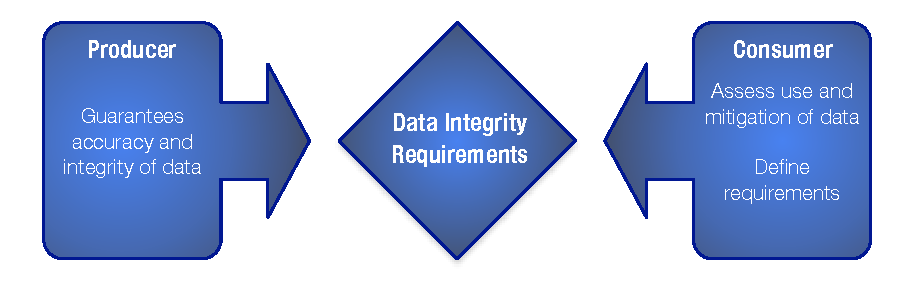
\includegraphics[width=0.75\textwidth]{images/producerconsumer}
  %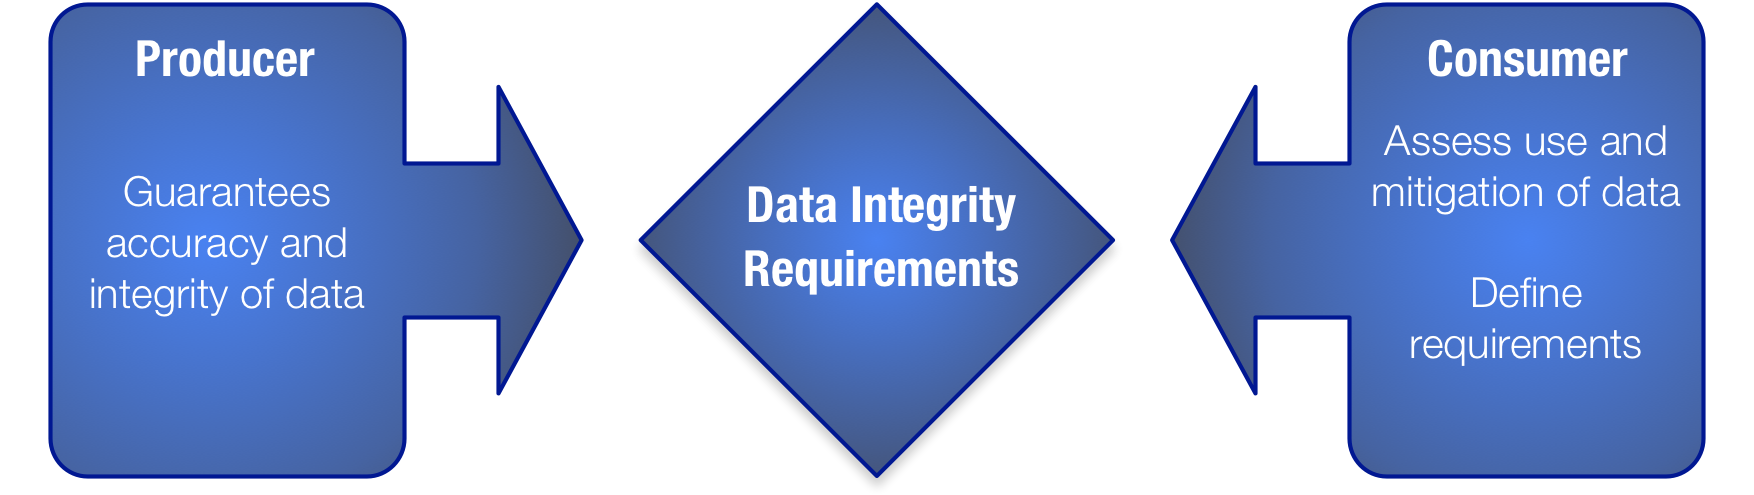
\includegraphics[width=0.75\textwidth]{images/producerconsumer.png}
  \caption{Consumer-focused \index{Integrity Property}integrity requirements}
  \label{fig:producerconsumer}
\end{figure}

The consumer assesses the use of the safety-related data. (In later phases of the Data Safety Management Process this information is used to define the required Data Properties: for example, how accurate a particular safety-related \index{Artefact, Data}Data Artefact must be.)

The producer investigates how the safety-related data is collected and what errors might occur. (Building on activities in later phases of the Data Safety Management Process, the producer can provide some form of guarantee, or level of confidence, that the safety-related data meets the specific data-related requirements.)

In some cases a producer will be providing safety-related data without any knowledge of a specific user (e.g., mapping data or generic databases that are sold to many users). In these cases the producer will need to make some assumptions about possible users, and then clearly state what level of \index{Integrity Property}integrity the data has been produced to. It is then up to the users to check whether the declared \index{Integrity Property}integrity matches their need.

\subsection{Data in System Lifecycles}
Like other components of a safety-related system, the safety dependency of data is dictated by the context in which it is used and the causal links that become established where loss of one or more of the required \index{Property!Data}properties can contribute to hazardous system states. For example, a given data set (say configuration data) could be used in a number of separate contexts such as:
\begin{itemize}
  \item prototyping a system to demonstrate solution feasibility of a safety-related system;
  \item development testing of a safety-related system; and
  \item live operational use of a safety-related system.
\end{itemize}

In these cases, the data set is the same but the context of its use changes the safety significance and therefore the level of assurance that it may require. It follows that the assessed \index{Assurance Level!Data}assurance level of a data set is also predicated on where and when in the lifecycle the data set will be applied. 

To illustrate this concept, a number of generic model lifecycles are discussed below. Note that these are not intended to be prescriptive or mandate the use of any particular model. Instead, they are being used to illustrate how the Data Safety Management Plan could articulate these lifecycle considerations.

\dsiwgTextBF{Development} The diagram in \autoref{fig:developmentlifecycle} represents a typical development lifecycle using an iterative development approach\footnote{The diagram is based on \acrshort{ibm}'s Rational Unified Process, an iterative software development\index{Software Development Process} process framework. The original diagram is in the public domain.}. In this model there are key phases as the system transitions from concept through to testable executable code. The process is iterative in that several cycles of functional elaboration, design, development and test may be run and these typically will focus on the areas of the system that bear most technical risk or comprise the key functional use cases so the client gets early visibility of the system. This early awareness allows feedback to be provided into the next iteration to help steer the solution to the client's actual needs. Traditional waterfall implementation can map onto this model on the basis that there is only one iteration in each phase and all activities in one phase need to be completed before progressing to the next.

\begin{figure}[htbp]
  \centering
  %\includegraphics[width=\textwidth]{images/developmentlifecycle}
  %\includegraphics[width=\textwidth]{images/developmentlifecycle_png600}
  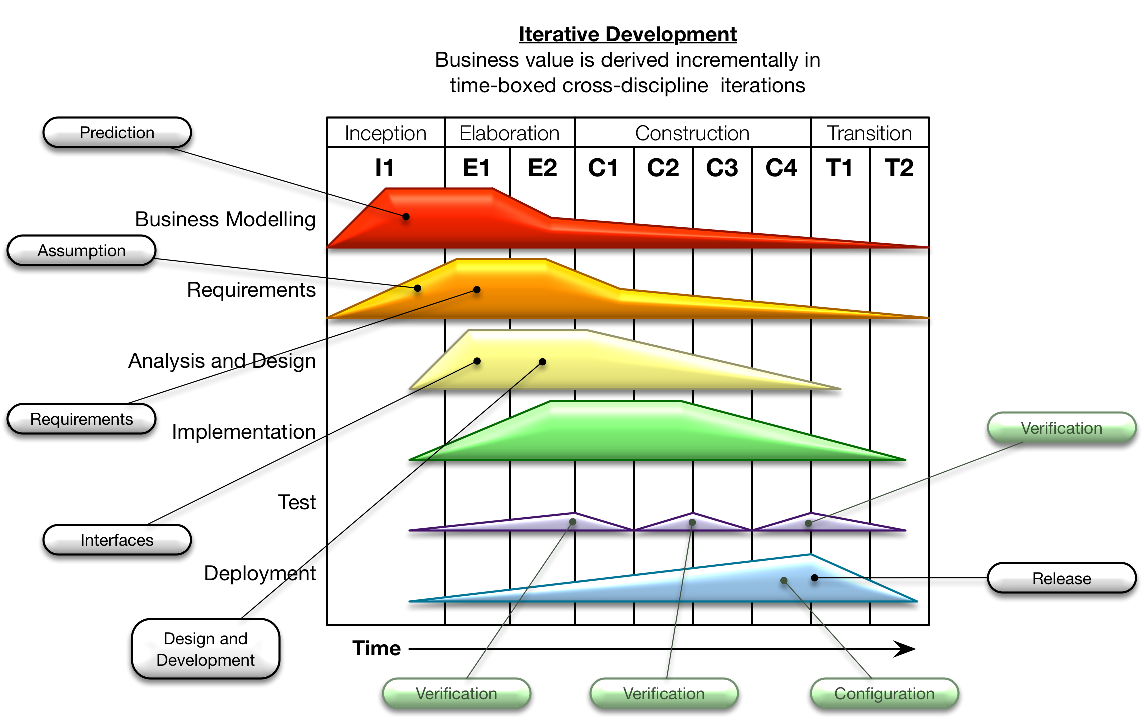
\includegraphics[width=\textwidth]{images/developmentlifecycleflat}
  \caption{Development lifecycle}
  \label{fig:developmentlifecycle}
\end{figure}

The model itself may vary depending on the specific needs of the project but the diagram illustrates that different Data Categories\index{Category!Data} become significant at different points of the process. 

\dsiwgTextBF{Operational} Once a system has been developed it will move into an operational lifecycle or indeed, if data safety has not previously been considered for an enterprise, then the system could already be in operational use. These operational lifecycles tend to be cyclical in nature; the diagram in \autoref{fig:operationallifecycle}\footnote{ITIL is a registered Trade Mark of AXELOS Limited. All rights reserved.} illustrates a typical model.

\begin{figure}[htbp]
  \centering
  %\includegraphics[width=0.9\textwidth]{images/operationallifecycle}
  %\includegraphics[width=0.9\textwidth]{images/operationallifecycle_png600}
  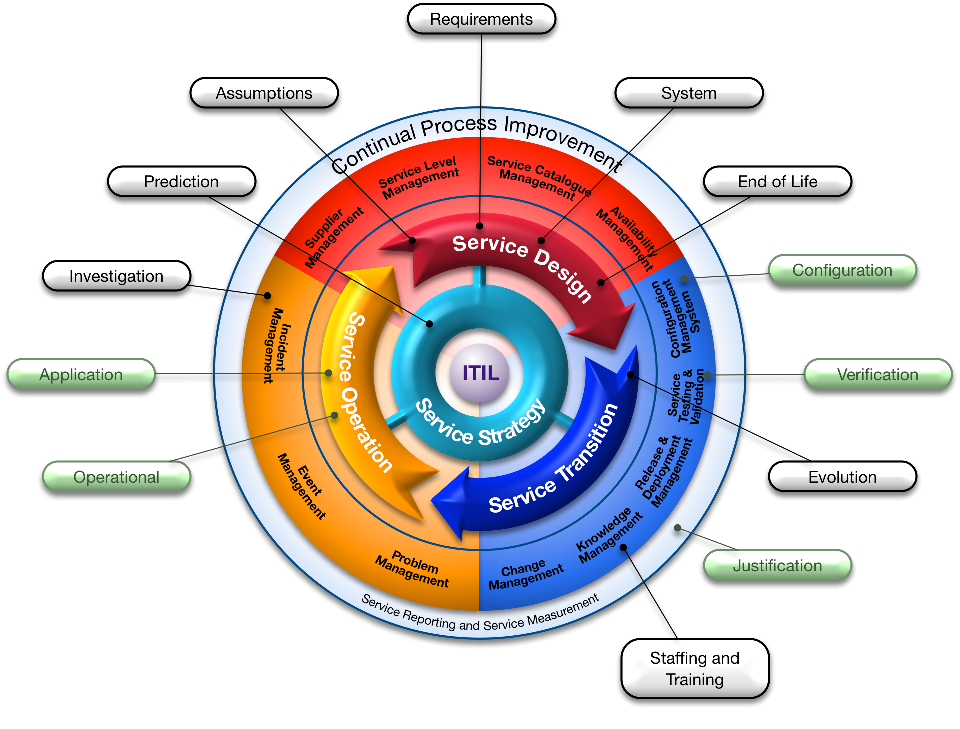
\includegraphics[width=0.9\textwidth]{images/operationallifecycleflat}
  \caption{Operational lifecycle}
  \label{fig:operationallifecycle}
\end{figure}

Again, specific Data \index{Category!Data} will come into play at different periods in the process. Documenting the relationship between process steps and Data Categories will therefore give clarity as to when a particular assurance technique needs to be applied.

\dsiwgTextBF{Data supply chains} The previous models relate to typical system supply and operate perspectives but there are also other data supply chains where a number of organizations engage in the procurement and use of safety-related data. These processes may include the development and operational lifecycles but a different model is required to fully represent the wider processes that are being employed. The diagram in \autoref{fig:dataacquisitionlifecycle} shows such a model representing a data acquisition lifecycle.

\begin{figure}[htbp]
  \centering
  %\includegraphics[width=\textwidth]{images/dataacquisitionlifecycle}
  %\includegraphics[width=\textwidth]{images/dataacquisitionlifecycle_png600}
  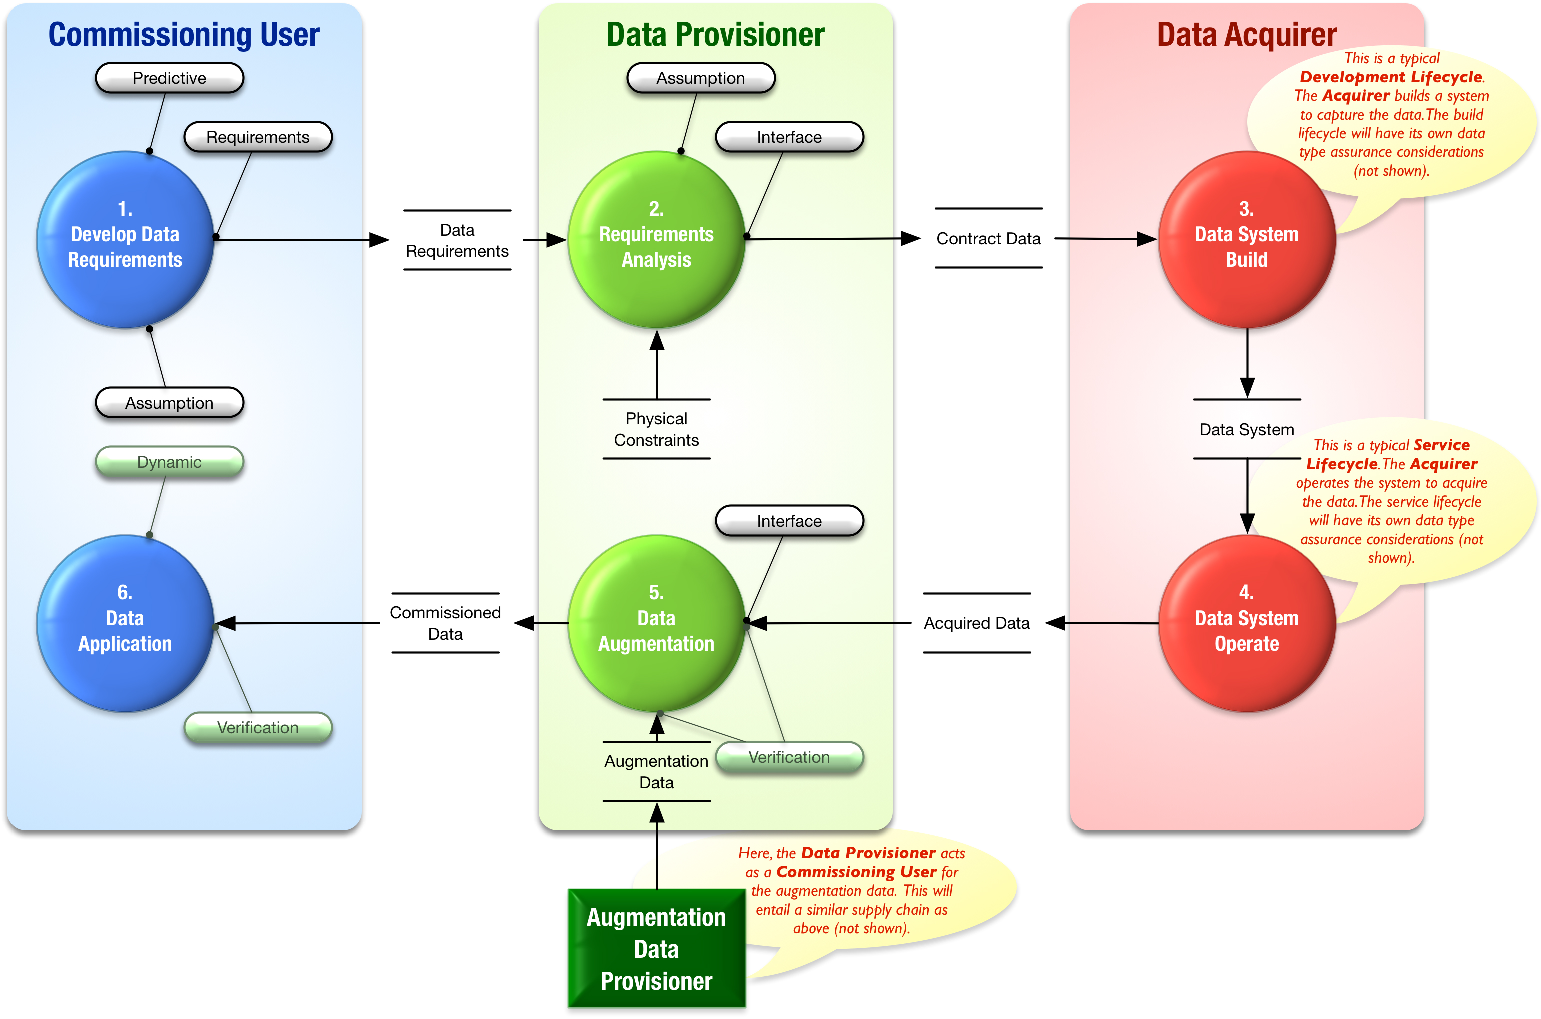
\includegraphics[width=\textwidth]{images/dataacquisitionlifecycleflat}
  \caption{Data supply chain}
  \label{fig:dataacquisitionlifecycle}
\end{figure}

This model represents the interactions between three key organizations:
\begin{itemize}
  \item The Commissioning User: the organization that has the need for the data;
  \item The Data Provisioner: the organization that will fulfil that need for data; and
  \item The Data Acquirer: the organization employed by the Data Provisioner to carry out physical collection of data.
\end{itemize}

Note that these may be three separate organizations, or they may be separate business units within the same, larger, organization.

In this supply chain, the Commissioning User is a Consumer of the data and the Data Acquirer is a Producer of data. The Data Provisioner acts both as a Consumer (from the Data Acquirer) and Producer (to the Commissioning User) of data. Similarly, an organization that augments data sets is both a Consumer and Producer of data in the supply chain.

The Commissioning User Requirement Analysis is the key process step where the Commissioning User's expectations for data (including \index{Fidelity/Representation Property}fidelity levels for associated \index{Property!Data}properties) are agreed with the Data Provisioner. The requirements may be adjusted because of physical constraints (e.g., loss of precision because of physical measuring device constraints) and may include additional requirements to augment the captured data with additional information (e.g., airport codes added to a measurement of a given runway length).

The Data Provisioner may employ a Data Acquirer to capture the data (e.g., to carry out a physical survey of a site). The acquisition phase may itself require a specialised system to be built to perform the capture and data refinement to meet the Data Provisioner's specifications. Such systems will then themselves be subject to the Development lifecycle model considerations discussed above. Likewise, the data augmentation phase may require further system development processes or indeed, could trigger an instance of the model again as the Data Provisioner acting as a Commissioning User.

Acquired and augmented data is then fed into the operational system that has been built for providing the service of generating the commissioned data. This system in its service provision role would then typically follow the Operational Lifecycle process model discussed earlier.

\subsubsection{Tool Assurance}
Tools in this context are considered anything that automates all or part of a process, for example, data creation or data transformation. Test tools are also included (i.e., the term is not limited to parts of an operational system).

Tools can impact data safety in different ways, depending on both their function and how they are to be used. For tools to be considered fit for purpose it is necessary to show that the tool meets its requirements in the context in which it is to be used. The activity to ensure a tool is fit for purpose is usually called ``tool qualification''.

The first step is to define the purpose for which the tool is required to be fit. Once that is done, and the tool's requirements are specified, there are three main strategies available for qualification:
\begin{itemize}
  \item Use evidence of a previous certification of the tool by a trusted third party (unlikely to be available in most industry sectors);
  \item Base tool qualification on the practices used when designing and developing the tool (only practicable for tools developed within the organization); and
  \item Use one of the available industry-specific guidance documents that admit \gls{cots} solutions, e.g., EUROCAE Document ED-215 (RTCA/DO-330) \cite{citation:ED215}.
\end{itemize}

%There is an alternative, risk-based and perhaps more feasible, approach. This involves assessing the potential risks presented by use of the tool and providing assurance that these risks are adequately managed. The method proceeds as follows:

%\begin{itemize}
%  \item Draft a procedure for the use of the tool to achieve the stated purpose;
%  \item Identify threats to data safety associated with using the tool;
%  \item Specify adequate mitigations\index{Mitigation} for each identified threat;
%  \item Augment and formally issue the tool requirements and the usage procedure to implement the specified  mitigations\index{Mitigation%};
%  \item Demonstrate that the tool and its mitigations\index{Mitigation} perform as expected; and
%  \item Provide a compelling assurance argument based on the previous steps and any other evidence that will improve confidence; for example:
%  \begin{itemize}
%    \item reputation of the supplier; 
%    \item configuration management of the tool, its settings and its documentation;
%    \item competence of the tool user; and
%    \item checks that are made on the tool's output.
%   \end{itemize}
%\end{itemize}

Further details on tool qualification are presented in \dsiwgRef{Appendix}{bkm:tools}.

\subsubsection{Test Data}
The generation of suitable test data is critical to verification of a safety system. The test data must include both representative ``normal'' values based on intended usage and also values which push at, and beyond, normal use to provoke hazards that the system might produce. This latter type of test data is particularly hard to generate: generally it must be credible, yet it must stress the system to react in a way that the preservation of \index{Property!Safety}safety properties can be assessed. 

In general, all the \index{Property!Data}properties of the test data should be considered and an assessment made as to whether breaking a property (e.g., introducing corrupt or late data) would cause a problem to the system. If it does, then specific test data should be produced to facilitate testing of this potential problem.

Some suggestions for test data for safety-related systems are:
\begin{itemize}
  \item Use of values on or around boundaries;
  \item Use of extreme values, way beyond what could be reasonably expected;
  \item Use of typical ``everyday'' values / sets;
  \item Some realistic but unexpected values;
  \item Try combinations of data values or items that are problematic together (e.g., inconsistent);
  \item If possible, use some values known to have caused problems in the past;
  \item Where appropriate, use values related to timing, rollover or date boundaries;
  \item Where possible, use white box values (i.e., those derived from an understanding of the system);
  \item Use a set of values with drift or bias over time;
  \item Use data sets with particular \index{Property!Statistical}statistical properties (e.g., distribution, patterns etc.);
  \item Use data which has incorrect formatting, ordering, or out of sequence, etc.; and
  \item Try data which has repeated sets of values or pseudo-random characteristics.
\end{itemize}
Typically very complex test data is derived from recorded live feeds of real data flows. While this data can be extremely useful for regression purposes, it should be recognised that it is unlikely to contain many outlying or boundary data items. Therefore it may need to be modified to test any hazardous situations; this modification can be difficult and may require sophisticated tools to both ensure correct \index{Property!Data}properties and injection of the intended faults (for instance to introduce a statistical bias to the data).

Simulator / emulator derived values can be useful, but again the issue is how realistic the values are: often the \index{Accuracy Property}accuracy, resolution or timing of simulated values may be different to real data.

Coverage with test data is something to consider. Sometimes the same data set is used for multiple test scenarios, when in fact it is not stressing all of them to the same degree. Test data coverage can be collected over requirements, code or design, but it is important not to forget hazards: coverage of the hazards and mitigations\index{Mitigation} identified in the hazard log is a key aim. 

In general some measure of the quality and suitability of the test data can be useful. This could be based on {Property!Statistical}statistical properties, coverage of hazards or coverage of requirements. 

Test data must show continued relevance, through systems evolution\index{Evolution!System} and over time. It is good practice to build up extensive regression suites containing coverage of all detected problems to date.

\subsubsection{Interfaces with Existing Assessments}\index{Interface!Assessment}
\paragraph{Data and Software}\index{Software vs. Data}
Although most people feel they have an intuitive understanding of the difference between software and data, upon closer examination the boundary is not always as clear as it may first appear.

Consider, for example, Java bytecode, which is operated on by a Java Virtual Machine. From one perspective, it could be argued that the Java bytecode is simply data. By extension, it could also be argued that the Java source code is also just data. This type of argument can be extended to suggest that any software\index{Software vs. Data} can, at least from one viewpoint, be considered as data. Conversely, think about the data used in a 3D printer, perhaps to produce a part for an aircraft. This data could be viewed as a program for the printer; that is, it could potentially be viewed as software. This type of argument can easily be extended across a range of situations, especially those relating to configuration data.

While they are interesting, and potentially important, these philosophical considerations should not detract from the practical issue: there are some aspects of data (using the term in a generic sense) that are often not explicitly addressed in standards. These are a consequence of features that are more readily apparent in data than in software\index{Software vs. Data}. Examples include:
\begin{itemize}
  \item It is easy for data to be reused in a range of contexts and despite appearances it is not trivial to translate an assurance argument that the data is fit for purpose from one context to another.
  \item It is not always clear who owns or is responsible for data, especially when data is shared and processed amongst a collection of disparate systems.
	\item Data often has a lifetime, that is a time after which it is no longer valid. This may be a strict cut off, or a more gradual degradation in the utility (or applicability) of the data.
  \item There is often a default value for data. While this can make systems easier to use and hence more productive it can be difficult to identify a default value that is appropriate for all circumstances.
  \item It can be easy to change data. In some circumstances this can give rise to a temptation to make uncontrolled and potentially untested changes. It can also allow data to be fraudulently changed after an accident.
\end{itemize}
In summary, data and software\index{Software vs. Data} are closely related and, as such, need to be considered together in system engineering activities, including system safety analyses. However, data and software emphasise different facets of risk and they are susceptible to different mitigation\index{Mitigation} approaches; this means there is also a need to adopt a data-focused perspective. It also means that \index{Assurance Level!Software}assurance levels related to software cannot be mapped directly to \index{Assurance Level!Data}\glspl{dsal}.

\paragraph{Data Safety and Security}
When generating high-level processes and techniques to manage the risks posed by data, it is worthwhile understanding the difference between the safety risks posed by accidental failure to preserve \index{Property!Data}Data Properties and the security risks posed by actors maliciously undermining the properties of data.

The relationship between safety and security, as engineering concepts, can be summarised by their relationships to cultural, developmental and aspirational \index{Property!System Development}properties of systems development.

Culturally, embedding both safety and security into an organization is seen as a key strategic goal for creating systems that are both safe and secure. Developmentally, safety and security are quality factors, generating transverse requirements that impact the entire system. Most importantly, at the aspirational level, both safety and security have the common goal of preventing harm from accidental and malicious interventions respectively.

For an organization aiming to create systems that are both safe and secure, these connections can be both a benefit and a burden. The shared goal of preventing harm means that both quality factors seek to identify routes to harm through analysis of the system being developed. This can result in shared processes and tools, which in turn can save time and money during systems development. However, safety and security interact in a more volatile way at the functional level. Security failings can undermine the safety case for a system and, conversely, \index{Safety Requirement}safety requirements can prevent the implementation of standard security solutions. For example, the German government published a report in 2014 into a fire at a steel works caused by a cyber attack that resulted in the control system being placed into an unsafe state and the safety system being unable to intervene (Section 3.3.1 of \cite{citation:DieLage} - in German). In addition, ``fail-safe'' states can often leave a system with exposed security vulnerabilities.

These links between safety and security infer that there are connections between the sub-categories of data safety and information security: both attempt to take a data-centric view of the system of interest in order to improve the associated quality factor; and both attempt to prevent harm through the preservation of the \index{Property!Data}properties of data within that system.

In the security domain, the three key properties of data considered are confidentiality, \index{Integrity Property}integrity, and availability. Confidentiality, the failure of which is termed ``Information Disclosure'' in the Microsoft Security Model, \cite{citation:leblanc2002writing} is typically not a safety concern as, without malicious intent, information sharing is not inherently unsafe. However, when considering systems where confidentiality is an important property, the interaction between data safety and security cannot be trivially resolved. For example, accidental disclosure of information can form part of a causal chain which leads to harm from a malicious actor.

Data \index{Integrity Property}integrity is a critical property for both domains. The Microsoft Security Model describes malicious removal of the property of \index{Integrity Property}integrity as ``tampering''. Whether by accident or through malicious intent, the potential harm from loss of data \index{Integrity Property}integrity can be disastrous to a safety-critical system, from the values of drug dosages to control system parameters. 

Data availability is also important to both domains. Loss of availability, or ``denial of service'' in the Microsoft Security Model, is another \index{Property!Data}property that can be lost accidentally or through malicious intervention. Loss of availability prevents systems from functioning properly and can result in undefined behaviour if not mitigated\index{Mitigation} by design.

Further guidance on the integration of safety and security can be found in a Code of Practice published by the IET
\cite{citation:IetCyber}.
The Code of Practice is written for engineers and engineering management to support their understanding of the issues
involved in ensuring that the safety responsibilities of an organization are addressed, in the presence of a threat of
cyber attack.

  %================================================================================
%       Safety Critical Systems Club - Data Safety Initiative Working Group
%================================================================================
%                       DDDD    SSSS  IIIII  W   W   GGGG
%                       D   D  S        I    W   W  G   
%                       D   D   SSS     I    W W W  G  GG
%                       D   D      S    I    WW WW  G   G
%                       DDDD   SSSS   IIIII  W   W   GGG
%================================================================================
%               Data Safety Guidance Document - LaTeX Source File
%================================================================================
%
% Description:
%   Machine Learning section.
%
%================================================================================
\section{\Glsfmtshort{ai} and \ecapitalisewords{\glsentrylong{ml}} (Informative)} \label{bkm:MachineLearning}

\dsiwgSectionQuote{Learning never exhausts the mind.}{Leonardo da Vinci}


\subsection{\ecapitalisewords{\glsentrylong{ml}} Training Data}\index{Machine Learning Data|textbf}
A complete discussion about the assurance of \gls{ml} /\gls{ai} algorithms is beyond the scope of this document.
However, as such algorithms are inherently data-driven, the Data Safety Guidance provides the following notes on good practice for \glspl{dataset} used for \gls{ml} / \gls{ai} applications.

The data for real-world \gls{ml} scenarios may be effectively infinite (for example, with self-driving cars, where the environment is largely unbounded) and can only be approximated by a finite number of scenarios.
Therefore it is crucial to have an extension process in place to extend the system when previously unknown situations are experienced. 
ISO~21448 \cite{citation:ISO21448} captures this process by introducing the term \gls{sotif} and requires the systematic handling of unknowns. Although specifically aimed at road vehicles, \gls{sotif} may be of interest to other domains.

For more general guidance on managing the safety of Autonomous Systems, please refer to the safety assurance objectives guidance produced by the SCSC \gls{saswg} \cite{citation:SASWG:Objectives}.

\subsection{Data Categories}
Three data categories are discussed: \cbstart\gls{ml} training data\index{Machine Learning Data} (the data used to train the model)\cbend,
\gls{ml} test data\index{Category!Data!Verification} (used to provide a measure the trained model’s \index{Accuracy Property}\gls{accuracy}), and \gls{ml}
validation data (used to independently verify the trained model).  

\subsection{Real-world Data}
It is important to obtain sufficient quantities of data for the training data. It is generally assumed that this is sufficiently representative of situations that could be encountered to allow the algorithm to generalise the appropriate behaviour for all encountered situations.  However, there are problems with real-life training data. Firstly, it is possible that rare, hazardous cases are never encountered during the capture of a \gls{dataset} (as those events have been engineered to be statistically unlikely) and are too dangerous, or expensive, to generate deliberately. Poor representation of rare cases in training data will result in a model that is insufficiently prepared to handle those important scenarios. Poor representation (or weighting) of rare cases in
\gls{ml} test data or \gls{ml}
validation data can result in error heuristics that do not provide adequate insight into the system’s performance\index{Performance, System} in rare situations. A second issue with real-world data is that amassing, understanding, verifying and validating it at scale is resource intensive.
Hence it is not just a case of more testing, a more cost-effective approach is needed. Some possible techniques are: artificial
\gls{ml}
test \gls{dataset} generation, data fault injection and simulation. It may well be more practicable to use simulated training data during the training phase to give more control and avoid the cost and effort of real-world testing. The issue then is how realistic the simulated data (and the associated simulation) can be. Note that artificial \glspl{dataset} can also be used to increase the frequency of rare events, thus biasing the algorithm to managing those rare events effectively, but doing so, could impair the ``sunny day'' performance\index{Performance, System} of the system.

\subsection{Sensor Data}
In many cases sensors will be on-board and embedded (e.g.\ on an automated vehicle) and will be subject to many real-world influences. Sensor data may be changed or degraded by both internal influences, e.g.\ system environment temperature, and external factors e.g.\ humidity, ambient light, weather conditions such as snow or fog, and rarely encountered extremes such as lightning or flood. 
Sensors may also suffer degradation due to ageing and specific faults due to their positioning, construction or configuration. Sensors may need to be diverse to increase resilience and give an overall more reliable output. Realistic data variations, informed by an understanding of likely sensor failure modes, need to be incorporated in the training \gls{dataset} (c.f.\ the AoA sensor in the Boeing 737 MAX~8, discussed in \autoref{bkm:incacc:737max8}).
Sensor fusion can effectively create ``composite data'', e.g.\ from merging of Lidar, Radar and Camera data; this will have different (and possibly hard to predict) \index{Property!Data}properties compared to the individual sensors.

\subsection{Data Coverage}
Some notion of data coverage, that is, how well the training data covers the intended operational domain, is needed: this could be based on use of all known \glspl{dataset}, all known hazardous situations or some other measure. White box techniques involved in exercising all connected sensors or coverage of nodes in a neural network may have some value. Regardless, it will be essential that the training data covers all required safety test scenarios.

\subsection{\Glsfmttext{dataset} Assurance}
There is a need to have assurance about the \glspl{dataset} themselves, including their configuration management. Assessment of the quality and suitability of the training \glspl{dataset} should be included in the safety argument.

The University of York has developed a method for the Assurance of Machine Learning for use in Autonomous Systems (AMLAS)
\cite{citation:machinelearning:amlas}.
The University's approach is intended to assist in the development of a compelling argument about a machine learning model,
to feed into a system safety case.

\subsection{Data Diversity}
The degree of data diversity is important. Common \glspl{item data} across \glspl{dataset} need to be avoided, especially across training and
\gls{ml}
validation data. Common data may include data derived from the same sources, environments, simulators, tools, techniques or mathematical models.

\subsection{\index{Property!Data}\ecapitalisewords{\glsentryplural{data property}}}
Bias, sufficiency and \index{Accuracy Property}\gls{accuracy} are all concerns with the data. \index{Fidelity/Representation Property}\cbstart\gls{fidelity}\cbend\ may also be a problem as modelling real-life sensor data is difficult.  Errors should be introduced for training: this may be by analytical means, by random, automated sampling of data to determine the degree of similarity between samples, or by means of deliberate insertion of known edge-cases. 
It is suggested that all the \index{Property!Data}\glspl{data property} mentioned in this guidance document are considered.

\subsection{Hallucinations}
\label{bkm:MachineLearning:Hallucinations}\index{Hallucinations|textbf}
%
The human brain can see and interpret patterns in unexpected ways, for example seeing a shadow that
suggests a monster is waiting to pounce, or seeing an animal in a cloud formation%
\footnote{These are not strictly hallucinations in the medical sense, but serve to illustrate
the issue with \gls{ai} interpretation of data.}.
\Gls{ai} tools can similarly interpret data in novel and unplanned ways, perhaps seeing patterns that a
human would not perceive, or seeing shapes in noise. However with \gls{ai} tools, hallucinations can appear
in two different ways --- in the interpretation of the question or instruction to perform, as well as
in the interpretation of the source data.
The problem is exacerbated in the case of \gls{ai} ``chatbots'', where the output presentation in natural
language can make the response seem authoritative and result in it being trusted, as though the
\gls{ai} chatbot is an expert in the field under consideration \cite{citation:chatbotsterrible:website}. 

The complete eradication of hallucinations may not be possible, so it can be dangerous to rely fully
on the output of an \gls{ai} without verification. Biases in the training data are regarded as a
significant cause of hallucinations, so selection of training data should include consideration
of its quality --- whether it is diverse, balanced and well structured
\cite{citation:halucinations:website}. In addition, evaluation of the resultant behaviour should be
assessed by humans, to achieve ``reinforcement learning with human feedback''
\cite{citation:howchatgptworks:website}.
The results of the assessments can then be fed back into the model,
thus fine-tuning it for its specific application.

Note that fine-tuning will generally only be possible for a specific application and/or a specific
environment. As with all safety analyses, it is critical that these be clearly defined.

We asked two different \glspl{ai} to comment on the risks that hallucinations present to data safety. Their responses were as presented in the
following two boxes:

\begin{aibox}%ChatGPT
  \Gls{ai} hallucinations can have significant implications for data safety and overall trust in \gls{ai} systems. Here are some key concerns:

Misinformation and Disinformation: If an \gls{ai} model generates incorrect or misleading \gls{information} (hallucinates), and this \gls{information} is used without verification, it can lead to the spread of misinformation. In sensitive areas like healthcare, finance, or law, this could have serious consequences.

Decision-Making Risks: In scenarios where \gls{ai} is used to aid decision-making, hallucinations can lead to incorrect or risky decisions. For instance, if a financial \gls{ai} advises on investments based on hallucinated data, it could lead to substantial financial losses.

Trust and Reliability Issues: Frequent hallucinations can undermine the trust in \gls{ai} systems. Users and organizations may become reluctant to rely on \gls{ai} for critical tasks if there's a significant risk of the \gls{ai} generating false \gls{information}.

Security Vulnerabilities: \gls{ai} hallucinations can be exploited in cybersecurity. For example, if an \gls{ai} system responsible for network security misinterprets data or hallucinates a threat, it could either overlook actual threats or allocate resources to non-existent threats.

Privacy Concerns: There’s a risk that an \gls{ai} model might inadvertently reveal or imply private \gls{information} in its outputs, especially if it has been trained on sensitive \glspl{dataset}. While not a hallucination in the traditional sense, this is related to the broader issue of how \gls{ai} handles and interprets data.

Ethical and Legal Implications: \gls{ai} hallucinations can lead to ethical and legal challenges, especially if they result in harm or damage. Determining liability in cases where AI-generated misinformation leads to real-world consequences is complex.

Bias and Fairness: Hallucinations can also be a reflection of biases in the training data. An \gls{ai} might generate outputs that are unfairly biased against certain groups or individuals, leading to ethical concerns and potential legal issues.

To mitigate these risks, it's crucial to have robust \gls{validation} and \gls{verification} processes, use \gls{ai} in conjunction with human oversight, continually update and improve \gls{ai} models with diverse and accurate data, and maintain transparency about the limitations and capabilities of \gls{ai} systems.
\end{aibox}

\begin{aibox}%Google Bard
  The implications of hallucinations for data safety are complex and far-reaching, spanning aspects of privacy, security, and misinformation. Here's a breakdown of some key concerns:

Privacy:

False generation of personal data: \gls{ai} hallucinations can fabricate personal \gls{information} (names, addresses, financial details) that doesn't actually exist, potentially violating privacy rights and harming individuals.
Exposure of sensitive data: If trained on sensitive data, hallucinations might leak this \gls{information} unintentionally, even if not explicitly instructed to do so. This could include medical records, financial data, or other confidential \gls{information}.
Security:

Creating vulnerabilities: Hallucinations might invent security flaws or exploits that don't actually exist, leading to wasted resources and potentially even vulnerabilities being introduced into real systems.
Misleading security assessments: If used for security testing, hallucinations could create false positives or negatives, providing inaccurate assessments of a system's security posture.
Misinformation:

Spreading false \gls{information}: \gls{ai}-generated hallucinations can easily spread misinformation, as they appear convincing and authoritative even if factually incorrect. This can have significant implications for public discourse, trust in institutions, and even manipulation.
Evolving deepfakes: Hallucinations could be used to create even more sophisticated deepfakes, making it harder to distinguish between real and fake content, further eroding trust and potentially influencing elections or other high-stakes situations.
Additional considerations:

Impact on trust: As reliance on \gls{ai} grows, hallucinations can erode trust in its outputs, making it harder to distinguish reliable \gls{information} from fabricated content.
Regulation and accountability: Establishing clear guidelines and accountability mechanisms for \gls{ai} systems prone to hallucinations is crucial to mitigate their risks.
Overall, addressing the implications of hallucinations for data safety requires a multi-pronged approach:

Developing robust and transparent \gls{ai} systems: Techniques like adversarial training and explainable \gls{ai} can help reduce hallucinations and improve transparency.
Implementing data governance and privacy measures: Strong data protection frameworks and responsible data handling practices are essential to minimize the risk of sensitive data exposure.
Promoting media literacy and critical thinking: Educating users to critically evaluate \gls{information}, regardless of its source, is crucial in the age of \gls{ai}-generated content.
Establishing ethical guidelines and regulations: Clear ethical frameworks and regulations for \gls{ai} development and deployment are necessary to ensure responsible use and mitigate potential risks.
By acknowledging the dangers of hallucinations and taking proactive steps to address them, we can minimize their impact on data safety and build trust in \gls{ai}-powered technologies.
\end{aibox}

\subsection{\Glsfmttext{dataset} Management}
\Glspl{dataset} will be large and complex and ensuring quality and \index{Consistency!Property}\gls{consistency} will be difficult. Measures will have to be taken to control, manage and archive large amounts of data. \Glspl{dataset} should be subject to formal change control and monitoring. Tools will be needed to manage the data.

\subsection{Optimization}
What is an optimal size of a training or
\gls{ml}
validation \gls{dataset}? A \gls{dataset} may contain many repeated or redundant values. If these do not add to the training outcome it is possible that some values may be removed. Also if there are ways in which the \gls{dataset} could be compressed or optimized then these should be considered to assist management and curation.

\subsection{Compliance}
A ``safety by compliance'' strategy for such data is difficult to implement as there are currently
few existing standards and little guidance for data in this area.
It is therefore difficult to quantify data sufficiency and as a result, no generally agreed ``ALARP'' principle for data.

It may be possible to demonstrate Data Safety through statistical methods,
such as when millions of representative miles have been driven.
However such approaches have generally been found insufficiently robust to support safety-critical systems in other domains
such as aviation, and so must be treated with caution.
The demonstration of compliance for the data is likely to require a compliance argument for the tools that produced the data,
the preservation of \index{Property!Data}\glspl{data property} as described within this document, and an update process such as that specified in ISO 21448 (SOTIF)
\cite{citation:ISO21448}.

\subsection{References}
This appendix provides only a brief overview of the issues around the application of data safety techniques to machine learning. It is based upon \gls{information} in the following documents, which should be consulted for further details:
\begin{itemize}
\item Assuring the Machine Learning Lifecycle: Desiderata, Methods, and Challenges \cite{citation:Ashmore2019}
\item Quantifying Data Set \index{Property!Data}Properties for Systematic Artificial Neural Network Classifier \Glsfmttext{verification} \cite{citation:Hond2020}
\item Safety Critical Integrity Assurance in Large Data Sets \cite{citation:Sutherland2020}
\end{itemize}

%  %================================================================================
%       Safety Critical Systems Club - Data Safety Initiative Working Group
%================================================================================
%                       DDDD    SSSS  IIIII  W   W   GGGG
%                       D   D  S        I    W   W  G   
%                       D   D   SSS     I    W W W  G  GG
%                       D   D      S    I    WW WW  G   G
%                       DDDD   SSSS   IIIII  W   W   GGG
%================================================================================
%               Data Safety Guidance Document - LaTeX Source File
%================================================================================
%
% Description:
%   AI and autonomy section.
%
%================================================================================
\section{AI and autonomy (Informative)} \label{bkm:autonomy}\index{AI|textbf}\index{Autonomy|textbf}

\cbstart
%
%\dsiwgSectionQuote{The first rule of any technology used in a business is that automation applied to an efficient operation will magnify the efficiency.
%  The second is that automation applied to an inefficient operation will magnify the inefficiency.}{Bill Gates}\todo{Pick a suitable quote}
%
\dsiwgSectionQuote{The potential benefits of artificial intelligence are huge, so are the dangers.}{Dave Waters}
%
%
%
\subsection{Job Displacement}\index{AI!Job displacement}
AI and automation can lead to the displacement of jobs, as machines can perform some tasks more efficiently than humans. This can have significant socioeconomic implications, including increased unemployment and wage stagnation in affected industries. The International Monetary Fund, (IMF), in January 2024, gave an estimate that AI will impact 40\% of jobs globally, and 60\% of highly skilled work, (ref 1). The report balances the already known complementary nature of AI to human work against the likely detrimental aspects. Unusually for technological advances, AI is expected to impact high-skilled jobs to a greater extent than manual skills. The report states, “advanced economies face greater risks from AI—but also more opportunities to leverage its benefits”. Labour requirements could significantly reduce, wages could be lower and of course jobs will disappear.  Managing Director of the IMF, Kristalina Georgieva, said that “AI will likely worsen overall inequality , a troubling trend that policymakers must proactively address to prevent the technology from further stoking social tensions.” (Ref 2). How economists are changing the standard growth view of economics and how engineering and other businesses can engage with such  developing problems is discussed in an article in the SCSC Newsletter edition 2024 (Ref 3). The data used to determine the impact of an AI system, especially when it affects currently underdeveloped nations must ensure that the social tension Georgieva refers to does not reach a breaking point. Like well digging, rail construction and careful dam placement, AI technology could raise many millions out of poverty if it is applied to benefit life on earth.

\begin{itemize}
\item Ref 1: International Monetary Fund, Staff Discussion Notes, “Gen-AI: Artificial Intelligence and the Future of Work”, Mauro Cazzaniga et al, (14/01/2024).
\item Ref 2: Western Daily Press, “AI to hit 40\% of jobs and will worsen inequality” Holly Williams, (16/01/2024) 
\item Ref 3: Engineering, Ethics and ‘Doughnut’ Economics, Nicholas Hales,  Safety Critical Systems Club Newsletter Feb 24 edition. Vol 32 Nos 2 SCSC-193
\end{itemize}

\subsection{Bias and Discrimination}\index{AI!Bias}\index{AI!Discrimination}
AI systems can inherit biases present in their training data, leading to discriminatory practices. For instance, facial recognition software has been shown to have higher error rates for people of certain racial and ethnic groups. At a very basic level, slight imperfections in coatings for car registration plates, easily ignored by humans, has made some number plates unrecognisable to automatic Number Plate Recognition cameras at car parks. This can be easily missed in training the system since it would have been difficult to anticipate the degree of training a system needs to recognise every possible imperfect state of a number plate. In this case advances are made from experience but there are many situations in which day one of a system’s deployment has to be near perfect. Training data sets should be vetted by committees, as safety usually is and should be always. That technique is more likely to bring out overlooked areas, obvious to someone on the committee but totally missed by others. Testing of developed systems should also cover the full range of possibilities, whether or not those involved in the development provide assurances, as assurances can hide failings.

\subsection{Loss of Human Skills}\index{Autonomy!Loss of human skills}
With AI taking over tasks such as navigation or memory-dependent activities, there is a risk that humans may lose certain skills that are not used regularly, potentially reducing cognitive abilities over time.  However, the opposite is also true, because driven by the threat of automation, many people could turn to artisan skills to create unique or less ubiquitous products providing an element of appealing individuality. This could turn supermarket check-out staff into, for instance entrepreneurial upholsterers, when and where all check-outs have become automated, or cosmetic developers. Regardless of whether or not skills are lost, it is certain that in order to verify and validate data intensive artificial intelligence systems someone will be required to maintain those basic skills to provide the assurance. To make a simple analogy, one cannot validate a French grammar correcting AI system if one does not speak French fluently.

\subsection{Security Risks}\index{AI!Security risks}
AI can be used to develop sophisticated cyber-attacks, and AI systems themselves can be vulnerable to such attacks. The integration of AI into critical infrastructure heightens the potential impact of these risks. The issue of autonomous vehicles in military applications has been discussed in an SCSC newsletter, (Ref 1) wherein a quote from a paper, “Formal Verification of Ethical Choices in an Autonomous System” (Ref 2), the following was written, “All participants in society are required to follow specific regulations and laws. An autonomous system cannot be an exception”. Given this as an accepted  principle it is then incumbent on engineers to design systems which follow ethical regulations. This presents difficulties and it demands that the most sophisticated sensors be employed on killer robots when decisions will need to be made as to whether or not to engage in an action which may result in death or excessive damage. Such examples are, firing a missile at a market square or bridge where known enemies are observed. At what point does the death of others not engaged in wrong doing become acceptable, known as collateral damage. Although it does not involve many robots, the conflict in the Gaza Strip is a prime example of this issue of what collateral damage is acceptable. That issue will be for the courts of justice to decide. Again it is important to stress that  the data used to train systems covers all possibilities, just as in human v  human conflict. If the machine is not programmed to make the decision, the machine must request clarification from human controllers. The issue is that it will almost certainly prove impossible to develop military killer systems that can be programmed with sufficient data to make every decision required in all circumstances without needing to consult humans, though direct accurate hits on isolated targets with little risk to the combatants of the targeting force is likely to remain an acceptable usage. But it would be sad if the governments of the world end up pitting machines they don’t understand against each other with all the horrendous possible consequences.
\begin{itemize}
\item Ref 1: “Autonomy’s Troubling Questions”, Nicholas Hales The Safety Critical Systems Club Newsletter Volume 27 Number 1, Winter 2018-19.
\item Ref 2: “Formal Verification of Ethical Choices in Autonomous Systems”, Robotics and Autonomous Systems Voll 77 (2015). L Dennis, M Fisher, M. Slavkovik and M Webster.
\end{itemize}

\subsection{Privacy Erosion}\index{AI!Privacy erosion}
AI's ability to analyse vast quantities of personal data can lead to erosion of privacy. For instance, AI can be used to make highly accurate predictions about individuals’ behaviours, preferences, and even future actions. To a limited extent this is already operational and desired by police forces wanting to identify faces and even the gait of wanted persons. The usual claim is that “If you are not doing anything wrong you have nothing to fear”. But many democracies are turning against the principle of eroding the human right to not  be constantly under surveillance or have already done so, trusting in the goodwill of the majority of citizens and accepting some policing techniques AI makes available are too close to fascism of the left or right wings of politics. A reply that may make advocates of surveillance policing change is to recommend they put cameras on the stairs in their house leading up to their bedrooms, just to check the wife is not having an affair with a colleague or the milkman because “If he or she is not doing anything wrong, they have nothing to fear”. Such a statement applied in the domestic situation may make the advocate awre that not everybody is happy about being the watchful eye of government. Even when the nation is not fascistic the creation of the network of cameras across a nation does provide the environment for a takeover by fascist elements. The Metropolitan Police  of London are using live facial recognition cameras. (Ref 1). Their policy is  “LFR cameras are focused on a specific area; when people pass through that area their images are streamed directly to the Live Facial Recognition system. This system contains a watchlist: a list of offenders wanted by the police and/or the courts, or those who pose a risk of harm to themselves or others.”  They currently assert that “LFR is not a ubiquitous tool that uses lots of CCTV cameras from across London to track every person’s movements”.  But a change of government, laws or the Mayor of London could change that. The risk is in the data being held may be abused or false, (police personnel have lied to get convictions in the past), the ability of the cameras to differentiate faces or gaits and the potential expansion of the system.

\begin{itemize}
\item Ref 1: \raggedright{\href{https://www.met.police.uk/advice/advice-and-information/fr/facial-recognition-technology/#:~:text=LFR\%20cameras\%20are\%20focused\%20on,harm\%20to\%20themselves\%20or\%20others}{https://www.met.police.uk/advice/advice-and-information/fr/facial-recognition-technology/\#:\~: text=LFR\%20cameras\%20are\%20focused\%20on,harm\%20to\%20themselves\%20or\%20others}}
\end{itemize}

\subsection{Control, Autonomy, Ethical and Moral Considerations}\index{AI!Control, Autonomy, Ethical and Moral Considerations}
As AI systems become more autonomous, there is a risk that they may act in unforeseen ways that are not aligned with human intentions or may be manipulated to act against human interests. Also there are significant ethical questions around AI, including the morality of decisions made by AI systems, particularly in life-and-death situations such as in autonomous vehicles or military applications. Although mainly concerned with military questions  “The Troubling Aspects of Autonomy” (Ref 1) discusses the issues of control that arise for dangerous life-threatening situations and is pertinent to non-military systems.
\begin{itemize}
\item Ref 1: “Autonomy’s Troubling Questions”, Nicholas Hales The Safety Critical Systems Club Newsletter Volume 27 Number 1, Winter 2018-19.
\end{itemize}

\subsection{Economic Inequality}\index{AI!Economic inequality}
The benefits of AI may accrue disproportionately to those who own the technology, potentially exacerbating economic inequality. Companies and nations that can invest in AI could gain significant economic advantages, leaving others behind. The likely beneficiaries are the developed economies. 40\% globally will be affected according to an IMF discussion paper and 60\% in the advanced technology world. Achim Steiner, Director of the Oxford Martin School, has said: “With new advances in the development of AI being made at a rapid pace, it is critical that as much importance is placed upon safety and ethical considerations as on technological progress”. In the fast world of competitive developments in AI which has now begun,  it is difficult to believe that the potential pitfalls are ever fully examined when, just as in more conventional engineering systems, the bottom line remains money gained through business success. Only regulation by governments and other authorities can be expected to be effective in limiting damage outside the bounds of AI systems. Some are now advocating a new form of economics known as Doughnut Economics as advocated by Professor Kate Raworth, Senior Teaching Associate at Oxford University’s Environmental Change Institute in her book on the subject, (Ref 1). A brief discussion of the some of the issues of such economics can be found in (Ref 2). There could be ways to support business in developing countries if AI tools are made available on smart phones at low cost to, for instance, African women’s business collectives. Data input and received from such applications will need to be safe and accurate if it is to benefit the less well-off of the world. Businesses must have good data to when using AI that provides reasonably accurate appraisals of outcomes from various actions. Ultimately, nobody should be left falling short of the social foundation that the Doughnut Economy declares the future ‘bottom line’ to be. In the Appendix to Raworth’s book, a table is given showing the issues that need addressing and declaring the sources. Such sources should be consulted for trusted data when new projects are developed. Typical statistic given would be an update to the books figures but similarly sourced, “Percentage of World population under-nourished = 11\% in years 2014-2016. 
\begin{itemize}
\item Ref 1: “Doughnut Economics – Seven ways to Think Like a 21st Century Economist” Professor Kate Raworth, Penguin Books, 2017 
\item Ref 2: Engineering, Ethics and ‘Doughnut’ Economics, Nicholas Hales,  Safety Critical Systems Club Newsletter Feb 24 edition. Vol 32 Nos 2 SCSC-193
\end{itemize}

\subsection{Dependency}\index{AI!Dependency}
Over-reliance on AI can lead to a lack of preparedness when systems fail. If critical infrastructure or services are AI-dependent, outages or malfunctions could have severe consequences. Simple growth of single point failure understanding applied to AI should mitigate a lot of the risk of loss of urgent data, like digital aircraft having three computer with a voting sub-system in overall control.

\subsection{Manipulation and Fake Content}\index{AI!Manipulation}\index{AI!Fake content}
AI can be used to create deep-fakes and synthetic media, which can be used to manipulate public opinion, perpetrate fraud, or spread misinformation. The Partnership for AI, (Ref 1),  have pursued the concept of there being a spectrum of harm from manipulated media. How this will all resolve is as yet unknown, the problem is in its relative infancy. With partners, a working definition arrived at is “any image or video with content or context edited along the “cheap fake” to “deepfake” spectrum (Data \& Society”) with the potential to mislead and cause harm” (Ref 2. A diagram and explanation of the spectrum can be found at Data and Society’s website (Ref 3). 12 Principles for labelling manipulated data can be found at the Partnership on AI (Ref 4) . As to whether any of this is enough, only time will tell. Much is seen in the news of demands for content providers to do better at eliminating bad data, be it manipulated or such things as sites encouraging suicide. However, it is worth noting that The Future of Humanity Institute (FHI), a research group within the Oxford Martin School, has joined the Partnership on AI and that organisation has as members many of the known big players in the data intensive media, Amazon, Apple, Google/DeepMind, Facebook, IBM and Microsoft. There goal is to formulate socially beneficial best practices for AI development. How much their belief in their achievements coincides with politicians requirements we must wait and see.  The Partnership for AI has produced a document “PAI’s responsible Practices for Synthetic Media”, (Ref 5), In which it is shown that current theory is that it is clear the best way to overcome fake media is by the organisations not trying to deceive anybody to have codes of practice. They seek to advance ethical and responsible behaviour. Synthetic Media, also known as generative media is defined as “..visual, auditory or multimodal content that has been generated or modified, commonly by artificial intelligence.”

It is accepted that legitimate use of such media may be for entertainment, art, satire, education and research to mention a few categories. Furthermore, techniques can be used legitimately or harmfully, there is no barrier. One recommendation for technology and infrastructure creators is “Aim to disclose in a manner that mitigates speculation about content, strives towards resilience to manipulation or forgery, is accurately applied and also when necessary, communicates uncertainty without furthering speculation”. The guide goes on to recommend practices for ‘Creators’ and ‘Distributors and Publishers’. Transparency and Disclosure are the main thrusts. It therefore appears that the legal definition for consumer risk will mirror goods purchase, Caveat Emptor, let the buyer beware, but with safeguards provided by companies wishing to take ethical stances.
\begin{itemize}
\item Ref 1: www.PartnershiponAI.org The Partnership on AI, Taking a Methodical Approach to Best Practices.
\item Ref 2: \href{https://datasociety.net/library/deepfakes-and-cheap-fakes/}
  {https://datasociety.net/library/deepfakes-and-cheap-fakes/}
\item Ref 3: \href{https://datasociety.net/wp-content/uploads/2019/09/Deep\_fakes\_spectrum.png}
  {https://datasociety.net/wp-content/uploads/2019/09/Deep\_fakes\_spectrum.png}
\item Ref 4: \href{https://partnershiponai.org/it-matters-how-platforms-label-manipulated-media-here-are-12-principles-designers-should-follow/}
  {https://partnershiponai.org/it-matters-how-platforms-label-manipulated-media-here-are-12- principles-designers-should-follow/}
\item Ref 5: \href{https://partnershiponai.org/wp-content/uploads/2023/02/PAI\_synthetic\_media\_framework.pdf}
  {https://partnershiponai.org/wp-content/uploads/2023/02/PAI\_synthetic\_media\_framework.pdf}
\end{itemize}

\subsection{Existential Risk}\index{AI!Existential risk}
In the long term, some theorists and scientists worry that the creation of super-intelligent AI could pose an existential risk to humanity if it becomes uncontrollable or its goals are misaligned with human values. This particular aspect of Data Safety with AI systems shows how important it is that the data used in AI systems reflects humanities values. The Doughnut Economics model uses, as the social foundation for humanity, twelve of the seventeen goals of the United Nations. Any AI system that is not trained, where relevant, using data that will ultimately achieve those goals, is almost certainly not an ethical system designed to align with the established values of the global humanitarian consciousness. Also many systems capable of destroying, such as  weapons, that have been granted autonomy, need to have been trained using the relevant data reflecting guidelines, in the military case, on conflict rules. Issues related to the military problems are discussed in Ref 1
\begin{itemize}
\item Ref 1:  “Autonomy’s Troubling Questions”, Nicholas Hales The Safety Critical Systems Club Newsletter Volume 27 Number 1, Winter 2018-19.
\end{itemize}

\subsection{An AI's view of the risks}
We asked an AI ``What sort of mistakes due to AI can be hard to detect?.'' The AI replied as follows:

\begin{aibox}
Artificial intelligence (AI) systems, while powerful and increasingly integral to many aspects of modern life, are not infallible. There are several types of mistakes or errors in AI systems that can be particularly hard to detect:

Subtle Data Bias: AI algorithms are often only as good as the data they are trained on. If this data contains biases, the AI can perpetuate or even amplify these biases. These biases can be subtle and deeply ingrained in the data, making them difficult to detect without thorough analysis.

Overfitting: This occurs when an AI model is too closely tailored to the specifics of its training data and fails to generalize well to new, unseen data. Detecting overfitting can be challenging because the model may perform exceptionally well on training data but poorly in real-world applications.

Black Box Models: Many advanced AI models, like deep neural networks, are often considered "black boxes" because their decision-making processes are not transparent or interpretable. This lack of transparency makes it difficult to understand why the AI made a certain decision and, consequently, to identify when it makes mistakes.

Contextual Misinterpretation: AI may not fully understand or consider the context in which data exists, leading to misinterpretations. These errors can be hard to detect because the AI's output may be logically consistent within the data it has, but contextually inappropriate.

Feedback Loops: In systems where AI output influences future input data, feedback loops can occur. For instance, in content recommendation algorithms, the system can get trapped in a loop of reinforcing its own biases, making it hard to detect errors in content filtering or recommendation.

Anomalous Data or Edge Cases: AI systems might struggle with data or situations that are significantly different from what they were trained on, known as edge cases. These anomalies can lead to errors that are hard to anticipate and detect because they occur outside the 'normal' operating parameters.

Errors in Complex Interactions: In systems where multiple AI models interact, errors can arise from the complex interplay between these systems. These errors can be particularly challenging to detect and diagnose because they may not arise from any single model but from the interaction between models.

Evolution of Language and Social Norms: AI systems trained on language data can become outdated as language and social norms evolve. Detecting when an AI system is no longer accurately interpreting or generating language according to contemporary standards can be difficult.

Misalignment with Human Values: AI might make decisions that are technically correct but misaligned with human ethics or values. These types of mistakes can be particularly hard to detect because they require nuanced understanding of human ethics, culture, and values.

To mitigate these issues, continuous monitoring, testing, diverse data sets, and incorporating explainability in AI systems are crucial. Additionally, involving human oversight and interdisciplinary expertise can help in detecting and correcting such hard-to-detect mistakes.
\end{aibox}
\cbend

%  %================================================================================
%       Safety Critical Systems Club - Data Safety Initiative Working Group
%================================================================================
%                       DDDD    SSSS  IIIII  W   W   GGGG
%                       D   D  S        I    W   W  G   
%                       D   D   SSS     I    W W W  G  GG
%                       D   D      S    I    WW WW  G   G
%                       DDDD   SSSS   IIIII  W   W   GGG
%================================================================================
%               Data Safety Guidance Document - LaTeX Source File
%================================================================================
%
% Description:
%   Appendix regarding Dark Data
%
%================================================================================
\section{Dark Data\index{Dark Data|textbf}\index{Data!Dark|see{Dark Data}} and Safety (Informative)} \label{bkm:darkdata}
%
%\dsiwgSectionQuote{Common sense tells us that the government's attempts to solve large problems more often create new ones. Common sense also tells us that a top-down, one-size-fits-all plan will not improve the workings of a nationwide health-care system that accounts for one-sixth of our economy}{Sarah Palin}
\dsiwgSectionQuote{\ldots we can be blind to missing data \ldots that can lead us to conclusions and actions that are mistaken, dangerous, or even disastrous.}{David Hand}

\subsection{Introduction}
This appendix outlines some of the safety implications arising from the issues identified by Prof. David Hand in his work on ``Dark Data'' presented in his book: ``Dark Data: Why What You Don't Know Matters'' \cite{citation:darkdata:hand} and website \cite{citation:darkdata:website}. Dark Data relates to data that is not available, but nevertheless is important, and indeed, in some cases, more important than the data that is available.

Unintentionally Donald Rumsfeld\index{Rumsfeld, Donald} popularised the concept of Dark Data with his famous speech:

\begin{quote}
\dsiwgTextIT{``…there are known knowns\index{Known Knowns}; there are things we know we know. We also know there are known unknowns\index{Known Unknowns}; that is to say we know there are some things we do not know. But there are also unknown unknowns\index{Unknown Unknowns}—the ones we don't know we don't know…''}
\end{quote}

\autoref{fig:lightanddark} neatly shows the dark varieties\index{Dark Data!Varieties} in grey:

\begin{figure}[htbp]
  \centering
  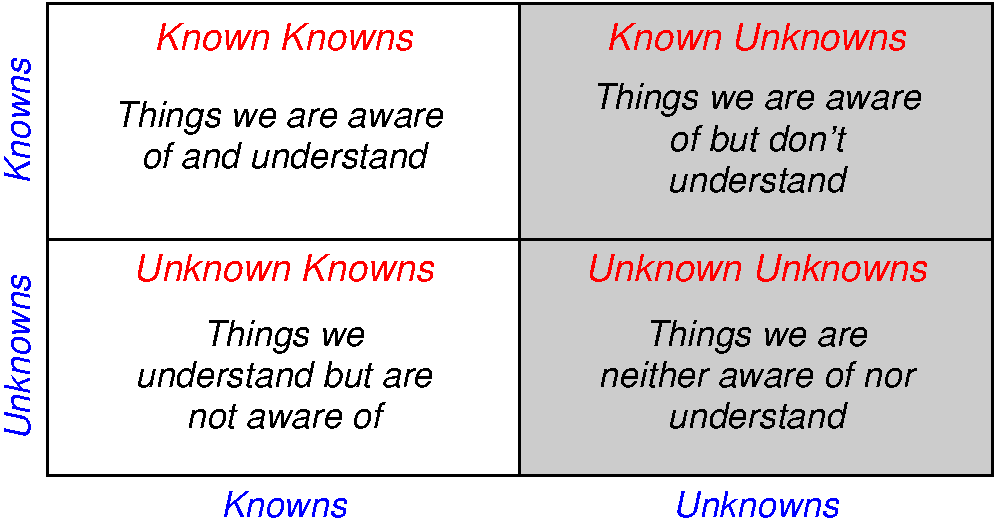
\includegraphics[width=\textwidth/2]{images/darkknowns.pdf}
  %\input{images/darkknowns.latex}
  \caption{Varieties of dark data\index{Dark Data!Varieties|textbf}}
  \label{fig:lightanddark}
\end{figure}\index{Unknown Knowns}

\subsection{Dark Data Example}
A meeting was held prior to the fatal Challenger disaster in January 1986, to decide whether the flight should go ahead due to the prevailing cold weather and concerns over the performance of O-ring seals at low temperatures. The decision to launch was made on the basis of the following data points that show the temperature at which previous O-ring problems had occurred.

\begin{figure}[htbp]
  \centering
  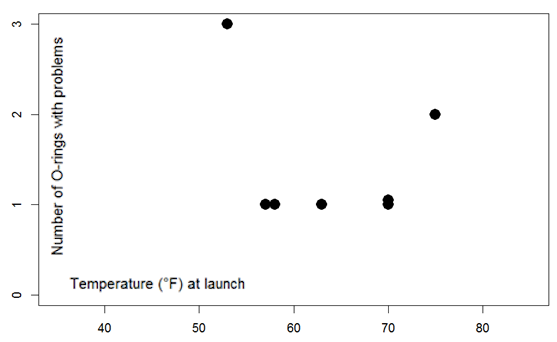
\includegraphics[width=\textwidth/2]{images/darkfailures}
  \caption{O-ring Failures by Temperature}
  \label{fig:o-ringfailures}
\end{figure}

On this basis, it was concluded that: 
``there is nothing irregular in the distribution of O-ring ‘distress’ over the spectrum of joint temperatures at launch between 53 degrees Fahrenheit and 75 degrees Fahrenheit.''
However, there was Dark Data in this dataset --- the data points that show the temperatures for successful launches when there were no O-ring problems were left out. These are shown as the red points in \autoref{fig:o-ringperformance}.

\begin{figure}[htbp]
  \centering
  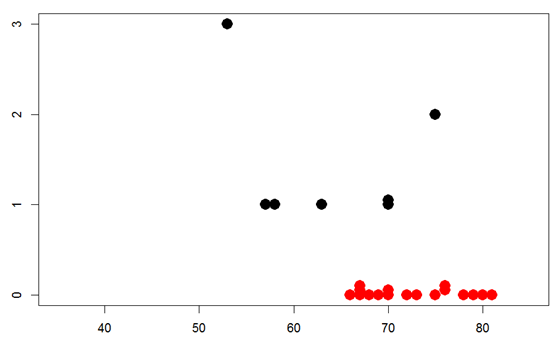
\includegraphics[width=\textwidth/2]{images/darkperformance}
  \caption{O-ring Performance by Temperature}
  \label{fig:o-ringperformance}
\end{figure}

When the Dark Data is included, there is an obvious correlation between temperature and O-ring failures and it is possible the decision to launch may have been different if this additional data had been presented.
\subsection{Dark Data Varieties\index{Dark Data!Varieties} and Safety Examples}
In his book, David introduces a taxonomy of 15 varieties of Dark Data. This section discuses each of these from a data safety perspective.

\subsubsection{Data We Know Are Missing: ``Known unknowns''}\index{Dark Data!Data We Know are Missing}\label{bkm:dark1}

This case is very common in safety justifications\index{Justification, Safety} where assurance information may be withheld for commercial reasons or does not exist, but we know, or are informed, that it isn’t available. Common examples include:
\begin{itemize}
  \item Assurance information for \gls{cots}\index{COTS} components is unavailable
  \item Information about legacy systems was never produced or is now lost
  \item ML training data restricted to a particular context of use
\end{itemize}
    If this is the case, it can be mitigated\index{Mitigation} in several ways, including use of warnings, training, restrictions of use, etc. Evidence can also be substituted with other more indirect assurance e.g.\ established organizational track-record in the sector, or audit reports.
    
\subsubsection{Data We Don’t Know Are Missing: ``Unknown unknowns''}\index{Dark Data!Data We Don't Know are Missing|textbf}\index{Unknown Unknowns}\label{bkm:dark2}
This is the most serious and far-reaching case. Occurrence is hopefully less common than case~\ref{bkm:dark1}, but it is important to acknowledge that it does happen. Some examples are:
\begin{itemize}
  \item The recent Covid-19 Track and Trace data loss (\autoref{bkm:incacc:covidexcel}), where the organization handling the data was unaware that rows were missing from a spreadsheet for some time is illustrated in \autoref {fig:darknewcases}
  \item Somebody knows a problem with a system but does not tell
  \item Machine learning training data\index{Machine Learning Data} missing edge / corner cases
  \item Key \index{Safety Requirement}safety requirements missed
  \item Change of use never anticipated
  \item Data loss which may be discovered after some period (or indeed never) 
  \item Test cases never thought of, so never created or executed
\end{itemize}

\begin{figure}[htbp]
  \centering
  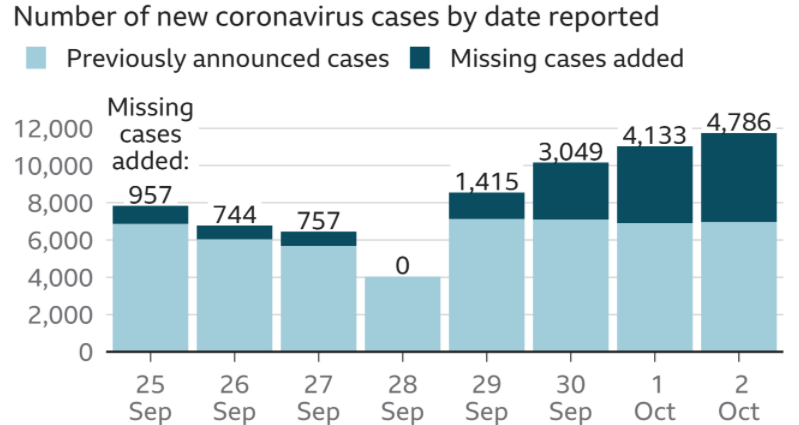
\includegraphics[width=\textwidth/2]{images/darknewcases}
  \caption{Covid-19 Track and Trace Data Loss}
  \label{fig:darknewcases}
\end{figure}

In many cases the loss may be discovered after some time, and it is incumbent on the organization involved to analyse the impact of the missing data over the time period, including subsequent decisions and actions. Its effects should not be underestimated. This case can fundamentally change the safety picture and is probably in the highest safety risk category.

Data that was missing can subsequently be found. The following options show possible approaches to handling this “rediscovered data”:
\begin{enumerate}[label=\color{dsiwgAccentColour}\roman*)]
  \item Apply the missing data
  \item Ignore the missing data 
  \item Mention that the data was missing but not take it into account, and 
  \item Perform an impact analysis on the missing data and then act according to the results
\end{enumerate}

\subsubsection{Choosing Just Some Cases}\index{Dark Data!Choosing Just Some Cases}\label{bkm:dark3}
This is where something or somebody has been selective. Examples might be:
\begin{itemize}
\item Selection of test runs that succeeded (ignoring failed runs and their diagnostics) 
  \item Selective sampling from sensors, or where the sampling intervals are chosen badly
  \item Incorrect filtering of the data, leaving out more cases than intended
  \item Using data from completed forms, finished tasks or only including data which,
    intentionally or not, meets some criteria which excludes the important data.
    This can lead to "Survivorship Bias",
    [Wikipedia ref:
      \href{https://en.wikipedia.org/wiki/Survivorship\_bias}
           {https://en.wikipedia.org/wiki/Survivorship\_bias}]
    of which the following article has a good example from WW2 aircraft where examining the bullet
    holes on aircraft returning from missions could have led to the wrong conclusion:
    \href{https://www.dgsiegel.net/talks/the-bullet-hole-misconception}
         {https://www.dgsiegel.net/talks/the-bullet-hole-misconception}
\end{itemize}
Note that with complex or informal criteria the effects could be as case~\ref{bkm:dark2}, i.e.\ you don’t know what has been left out.

Mitigations\index{Mitigation} include use of peer review, independent teams, and audits. It is important to ask questions and challenge the data selected to be sure it can be justified.
\subsubsection{Self-Selection}\index{Dark Data!Self-selection}\label{bkm:dark4}
This is considered to be similar to case~\ref{bkm:dark3}, but could be even more informal or ambiguous. Again mitigations\index{Mitigation} include: use of peer review, independent teams, and audits.

\subsubsection{Missing What Matters}\index{Dark Data!Missing What Matters|textbf}\label{bkm:dark5}
This was considered similar to case~\ref{bkm:dark2} in impact terms, and might well be considered the “Elephant in the Room”. Examples might be:
\begin{itemize}
\item Measuring the wrong things, e.g.\ poor safety metrics / indicators
  \item Too much data to deal with or analyse, so some is ignored
  \item Too much filtering or processing, so losing information along the way
  \item Being too close to the data, i.e.\ the “wood for the trees”. This is when the detail masks the overall issue with data, e.g.\ a slow trend or bias masked by peaks.
\end{itemize}

Mitigations\index{Mitigation} include independence as~\ref{bkm:dark3} and~\ref{bkm:dark4} but also “taking a step back” to look at the bigger picture.
\subsubsection{Data Which Might Have Been}\index{Dark Data!Data Which Might Have Been}\label{bkm:dark6}
This is where it is impossible to obtain the relevant data as a consequence of how the system/scenario is constructed. This was considered an interesting and important case.

This could for example, be due to an inappropriate system architecture e.g.\ single data channel when a multiple channel approach should have been used, such as in the \index{Boeing 737}Boeing 737 MAX~8 accidents (see section H.2). It is therefore important that Mitigations\index{Mitigation} are in place at design time, as they are often very difficult to retro-fit.

Mitigations\index{Mitigation} include assessing the data collection opportunities gained or lost from the design or architectural approach --- at design time.

\subsubsection{Changes with Time}\index{Dark Data!Changes With Time}\label{bkm:dark7}
This is a common problem in a safety context. Data in safety systems often becomes obsolete or out of date and may still be mistakenly used. Some examples are:
\begin{itemize}
\item System configuration data not kept up to date as software\index{Software Changes} or hardware changes
  \item Medical drug interaction databases
  \item Software patches requiring updates to configuration or system data, which is not always done
\end{itemize}

Mitigations\index{Mitigation} include keeping critical data up to date and regularly refreshed, and knowing how old the data is in the first place.

\subsubsection{Definitions of Data}\index{Dark Data!Definitions of Data}\label{bkm:dark8}
This was considered a common case for systems with databases or those exchanging data with external systems, e.g.
\begin{itemize}
\item Taxonomies e.g.\ in machine learning categorisation schemes
  \item Data schemas in medical record systems 
  \item Interface specifications\index{Interface!Specification} and data definitions\index{Data!Definition}, which often evolve over time. These can render old data obsolete / subject to misinterpretation, and often needing migration/translation or re-interpretation.
\end{itemize}

Mitigations\index{Mitigation} include keeping a list of known changes / incompatibilities and documenting the changes or fixes that have to be applied to make the data usable or consistent.

\subsubsection{Summaries of Data}\index{Dark Data!Summaries of Data}\label{bkm:dark9}
This is often seen in data about safety systems and projects:
\begin{itemize}
\item Safety metrics or indicators where data is aggregated to create a composite value
  \item Data fusion across multiple sensors
Summaries can be misleading or cause “boundary reactions”, e.g. Red-Amber boundary.
\end{itemize}

Mitigations\index{Mitigation} include thinking about what missing data could cause (i.e.\ performing sensitivity analysis) --- for instance, what decisions might be made erroneously due to certain data values being omitted, late or slightly perturbed.

\subsubsection{Measurement Error and Uncertainty}\index{Dark Data!Measurement Error and Uncertainty}\label{bkm:dark10}
Sensors can degrade and fail over time, especially in harsh environments such as automotive, marine or aviation:
\begin{itemize}
\item Sensors may feed faulty or biased data into systems
  \item Sampling techniques can cause some artefacts in themselves
  \item Interval polling interval can lead to misleading readings
  \item Data fusion can be impacted if multiple sensor values are combined
\end{itemize}

Hence sensors need to be regularly maintained and calibrated or replaced, and their interfaces\index{Interface!Sensor} need to be able to detect any problems and report faults. 

\subsubsection{Feedback and Gaming}\index{Dark Data!Feedback and Gaming}\label{bkm:dark11}
This can often happen in safety justifications\index{Justification!Safety} or test case production:
\begin{itemize}
\item Early production of a safety argument could lead to only those artefacts that support the claim being generated, e.g.\ requirements-based testing vs.\ stress testing
  \item Confirmation bias in safety justifications\index{Justification, Safety} and can cause over-optimism
\end{itemize}

Mitigations\index{Mitigation} include the use of dialectic argument approaches (where both positive and negative cases can be considered). It is also useful to get a second opinion, independent review or a ‘fresh pair of eyes’ to check the justification.

\subsubsection{Information Asymmetry}\index{Dark Data!Information Assymetry}\label{bkm:dark12}
This is common where there are multiple stores or sources of the same data:
\begin{itemize}
\item Multiple / backup databases where they are not kept in sync
  \item Image recognition systems that learn, but fail to share data
  \item Issues of divergence of data across multiple sources.
\end{itemize}

Comparisons, reviews and data audits may help in these cases. In general the issue of divergence across multiple data sources needs to be recognized and addressed in the most appropriate technical, and ideally automated, way.

\subsubsection{Intentionally Darkened Data}\index{Dark Data!Intentionally Darkened Data}\label{bkm:dark13}
This can and does happen, e.g.
\begin{itemize}
\item Defence, security and government sectors where data is purposefully hidden or destroyed
  \item Records intentionally deleted after an accident to cover up what really happened
\end{itemize}

This can be mitigated\index{Mitigation} using appropriate technical measures (e.g.\ blockchain, digital signatures, off-site backups), and also robust procedures with oversight.

\subsubsection{Fabricated and Synthetic Data}\index{Dark Data!Fabricated and Synthetic Data}\label{bkm:dark14}
Fabrication (i.e.\ making up the data) is surprisingly common, e.g.\ in medical, policing and maritime sectors. Sometimes it is created with the best of intentions as it was not produced or collected at the right time and is now required (e.g.\ for an audit), but sometimes it is created to mask a problem. Synthetic data is often used where there are difficulties in producing enough real data with the right characteristics:
\begin{itemize}
\item Data is retrospectively entered / patched to make a “clean” record
  \item Synthetic autonomous vehicle training databases can have issues with artificial data if not realistic
\end{itemize}

Possible mitigations\index{Mitigation} include comparisons with current real-world data and checking with historical data.

\subsubsection{Extrapolating Beyond Your Data}\index{Dark Data!Extrapolating Beyond Your Data}\label{bkm:dark15}
Systems, especially machine learning systems (see Appendix J) have to cope with values outside of their training data\index{Machine Learning Data}, but the outcomes may be unexpected:
\begin{itemize}
\item Bizarre results from recognition / detection systems may result
\end{itemize}

Mitigations\index{Mitigation} include use of machine learning training data\index{Machine Learning Data} containing edge/corner cases, boundary cases, and testing well beyond normal or acceptable ranges to give insight into the system degradation behaviour.

\subsection{Summary}
Dark Data is a very useful way of thinking about problems and solutions. It is important to always think of the bigger picture, considering what information is not known:

\begin{itemize}
  \item What might have been left out, intentionally or otherwise?
  \item What might be missing due to the way things are done (or the way those things are being executed)?
  \item Could missing items cause any safety problems?
  \item What is outside of the defined operational domain?
  \item Can you present your results / outputs in a way that shows the dark data?
\end{itemize}

\subsection{Further Reading}
A number of resources are available for further information on how Dark Data relates to data safety:
\begin{itemize}
\item The October 2020 edition of the SCSC Newsletter \cite{citation:SCSC160} contains articles both by David Hand and on Dark Data Safety.
  \item A presentation on Dark Data given by David Hand to the \gls{dsiwg} \cite{citation:darkdata:presentation1};
  \item A presentation by Mike Parsons given at the University of York \cite{citation:darkdata:presentation2}.
\end{itemize}

  %================================================================================
%       Safety Critical Systems Club - Data Safety Initiative Working Group
%================================================================================
%                       DDDD    SSSS  IIIII  W   W   GGGG
%                       D   D  S        I    W   W  G   
%                       D   D   SSS     I    W W W  G  GG
%                       D   D      S    I    WW WW  G   G
%                       DDDD   SSSS   IIIII  W   W   GGG
%================================================================================
%               Data Safety Guidance Document - LaTeX Source File
%================================================================================
%
% Description:
%   Appendix regarding Dark and Dazzle Data
%
%================================================================================
\section{Dark Data and Dazzle Data (Informative)}%
\label{bkm:darkdazzledata}
%
%\dsiwgSectionQuote{Common sense tells us that the government's attempts to solve large problems more often create new ones. Common sense also tells us that a top-down, one-size-fits-all plan will not improve the workings of a nationwide health-care system that accounts for one-sixth of our economy}{Sarah Palin}
\dsiwgSectionQuote{\ldots we can be blind to missing data \ldots that can lead us to conclusions and actions that are mistaken, dangerous, or even disastrous.}{David Hand}

\subsection{Introduction}
Dark and Dazzle data may be viewed as two sides of the same coin. In the former data is hidden, whilst in the latter the important information is hidden by an abundance of other data.

\subsection{Dark Data}%
\index{Dark Data|textbf}\index{Data!Dark|see{Dark Data}}%
\label{bkm:darkdata}
%
\subsubsection{Introduction to Dark Data}
This appendix outlines some of the safety implications arising from the issues identified by Prof. David Hand in his work on ``Dark Data'' presented in his book: ``Dark Data: Why What You Don't Know Matters'' \cite{citation:darkdata:hand} and website \cite{citation:darkdata:website}. Dark Data relates to data that is not available, but nevertheless is important, and indeed, in some cases, more important than the data that is available.

Unintentionally Donald Rumsfeld\index{Rumsfeld, Donald} popularised the concept of Dark Data with his famous speech:

\begin{quote}
\dsiwgTextIT{``…there are known knowns\index{Known Knowns}; there are things we know we know. We also know there are known unknowns\index{Known Unknowns}; that is to say we know there are some things we do not know. But there are also unknown unknowns\index{Unknown Unknowns}—the ones we don't know we don't know…''}
\end{quote}

\autoref{fig:lightanddark} neatly shows the dark varieties\index{Dark Data!Varieties} in grey:

\begin{figure}[htbp]
  \centering
  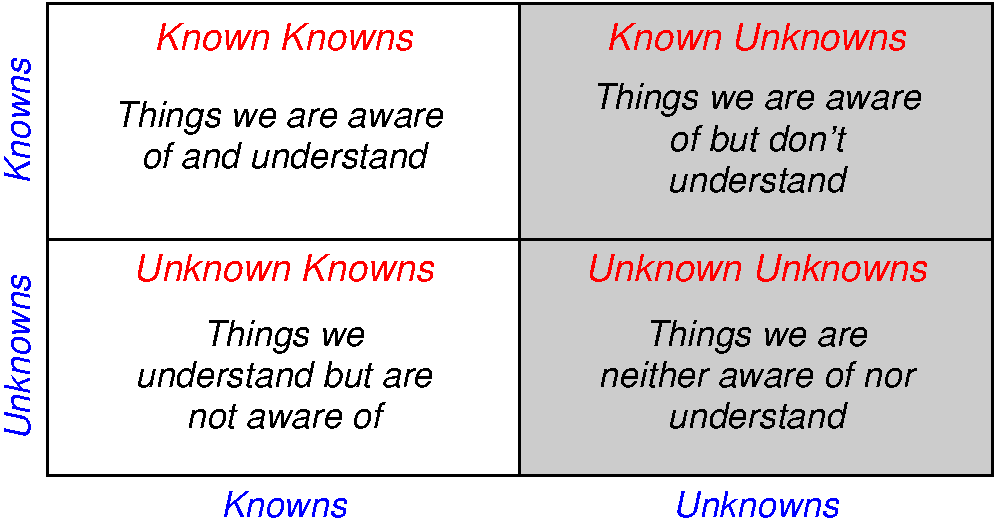
\includegraphics[width=\textwidth/2]{images/darkknowns.pdf}
  %\input{images/darkknowns.latex}
  \caption{Varieties of dark data\index{Dark Data!Varieties|textbf}}
  \label{fig:lightanddark}
\end{figure}\index{Unknown Knowns}

\subsubsection{Dark Data Example}
A meeting was held prior to the fatal Challenger disaster in January 1986, to decide whether the flight should go ahead due to the prevailing cold weather and concerns over the performance of O-ring seals at low temperatures. The decision to launch was made on the basis of the following data points that show the temperature at which previous O-ring problems had occurred.

\begin{figure}[htbp]
  \centering
  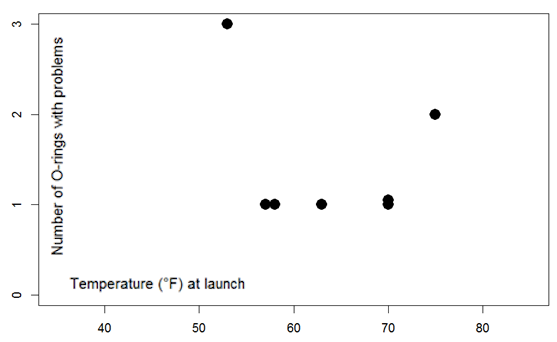
\includegraphics[width=\textwidth/2]{images/darkfailures}
  \caption{O-ring Failures by Temperature}
  \label{fig:o-ringfailures}
\end{figure}

On this basis, it was concluded that: 
``there is nothing irregular in the distribution of O-ring ‘distress’ over the spectrum of joint temperatures at launch between 53 degrees Fahrenheit and 75 degrees Fahrenheit.''
However, there was Dark Data in this dataset --- the data points that show the temperatures for successful launches when there were no O-ring problems were left out. These are shown as the red points in \autoref{fig:o-ringperformance}.

\begin{figure}[htbp]
  \centering
  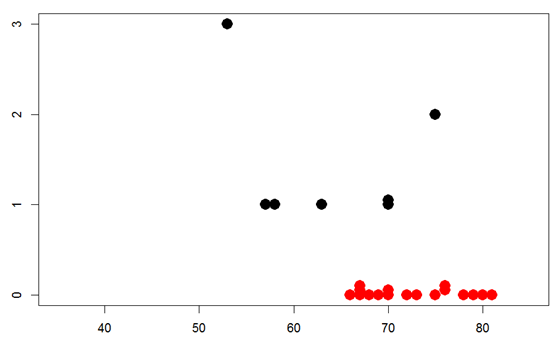
\includegraphics[width=\textwidth/2]{images/darkperformance}
  \caption{O-ring Performance by Temperature}
  \label{fig:o-ringperformance}
\end{figure}

When the Dark Data is included, there is an obvious correlation between temperature and O-ring failures and it is possible the decision to launch may have been different if this additional data had been presented.

\subsubsection{Dark Data Varieties\index{Dark Data!Varieties} and Safety Examples}
In his book, David introduces a taxonomy of 15 varieties of Dark Data. This section discuses each of these from a data safety perspective.

\paragraph{Data We Know Are Missing: ``Known unknowns''}\index{Dark Data!Data We Know are Missing}\label{bkm:dark1}

This case is very common in safety justifications\index{Justification, Safety} where assurance information may be withheld for commercial reasons or does not exist, but we know, or are informed, that it isn’t available. Common examples include:
\begin{itemize}
  \item Assurance information for \gls{cots}\index{COTS} components is unavailable
  \item Information about legacy systems was never produced or is now lost
  \item \Gls{ml} training data restricted to a particular context of use
\end{itemize}
    If this is the case, it can be mitigated\index{Mitigation} in several ways, including use of warnings, training, restrictions of use, etc. Evidence can also be substituted with other more indirect assurance e.g.\ established organisational track-record in the sector, or audit reports.
    
\paragraph{Data We Don’t Know Are Missing: ``Unknown unknowns''}\index{Dark Data!Data We Don't Know are Missing|textbf}\index{Unknown Unknowns}\label{bkm:dark2}
This is the most serious and far-reaching case. Occurrence is hopefully less common than case~\ref{bkm:dark1}, but it is important to acknowledge that it does happen. Some examples are:
\begin{itemize}
  \item The recent Covid-19 Track and Trace data loss (\autoref{bkm:incacc:covidexcel}), where the organisation handling the data was unaware that rows were missing from a spreadsheet for some time is illustrated in \autoref {fig:darknewcases}
  \item Somebody knows a problem with a system but does not tell
  \item Machine learning training data\index{Machine Learning Data} missing edge / corner cases
  \item Key \index{Safety Requirement}safety requirements missed
  \item Change of use never anticipated
  \item Data loss which may be discovered after some period (or indeed never) 
  \item Test cases never thought of, so never created or executed
\end{itemize}

\begin{figure}[htbp]
  \centering
  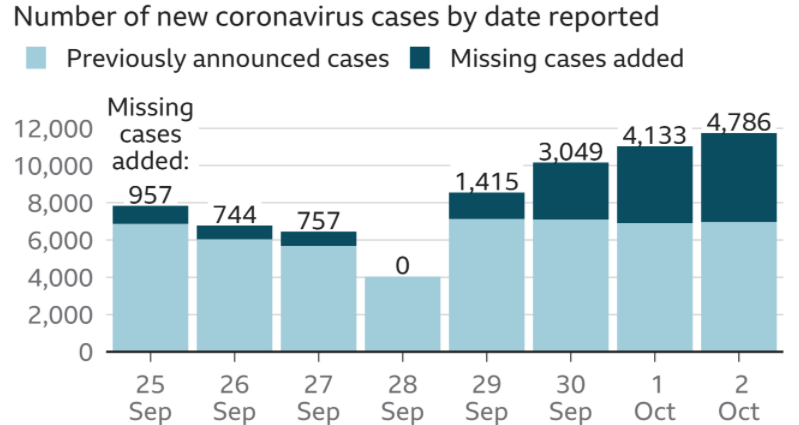
\includegraphics[width=\textwidth/2]{images/darknewcases}
  \caption{Covid-19 Track and Trace Data Loss}
  \label{fig:darknewcases}
\end{figure}

In many cases the loss may be discovered after some time, and it is incumbent on the organisation involved to analyse the impact of the missing data over the time period, including subsequent decisions and actions. Its effects should not be underestimated. This case can fundamentally change the safety picture and is probably in the highest safety risk category.

Data that was missing can subsequently be found. The following options show possible approaches to handling this “rediscovered data”:
\begin{enumerate}[label=\color{dsiwgAccentColour}\roman*)]
  \item Apply the missing data
  \item Ignore the missing data 
  \item Mention that the data was missing but not take it into account, and 
  \item Perform an impact analysis on the missing data and then act according to the results
\end{enumerate}

\paragraph{Choosing Just Some Cases}\index{Dark Data!Choosing Just Some Cases}\label{bkm:dark3}
This is where something or somebody has been selective. Examples might be:
\begin{itemize}
\item Selection of test runs that succeeded (ignoring failed runs and their diagnostics) 
  \item Selective sampling from sensors, or where the sampling intervals are chosen badly
  \item Incorrect filtering of the data, leaving out more cases than intended
  \item Using data from completed forms, finished tasks or only including data which,
    intentionally or not, meets some criteria which excludes the important data.
    This can lead to "Survivorship Bias",
    [Wikipedia ref:
      \href{https://en.wikipedia.org/wiki/Survivorship\_bias}
           {https://en.wikipedia.org/wiki/Survivorship\_bias}]
    of which the following article has a good example from WW2 aircraft where examining the bullet
    holes on aircraft returning from missions could have led to the wrong conclusion:
    \href{https://www.dgsiegel.net/talks/the-bullet-hole-misconception}
         {https://www.dgsiegel.net/talks/the-bullet-hole-misconception}
\end{itemize}
Note that with complex or informal criteria the effects could be as case~\ref{bkm:dark2}, i.e.\ you don’t know what has been left out.

Mitigations\index{Mitigation} include use of peer review, independent teams, and audits. It is important to ask questions and challenge the data selected to be sure it can be justified.

\paragraph{Self-Selection}\index{Dark Data!Self-selection}\label{bkm:dark4}
This is considered to be similar to case~\ref{bkm:dark3}, but could be even more informal or ambiguous. Again mitigations\index{Mitigation} include: use of peer review, independent teams, and audits.

\paragraph{Missing What Matters}\index{Dark Data!Missing What Matters|textbf}\label{bkm:dark5}
This was considered similar to case~\ref{bkm:dark2} in impact terms, and might well be considered the “Elephant in the Room”. Examples might be:
\begin{itemize}
\item Measuring the wrong things, e.g.\ poor safety metrics / indicators
  \item Too much data to deal with or analyse, so some is ignored
  \item Too much filtering or processing, so losing information along the way
  \item Being too close to the data, i.e.\ the “wood for the trees”. This is when the detail masks the overall issue with data, e.g.\ a slow trend or bias masked by peaks.
\end{itemize}

Mitigations\index{Mitigation} include independence as~\ref{bkm:dark3} and~\ref{bkm:dark4} but also “taking a step back” to look at the bigger picture.

\paragraph{Data Which Might Have Been}\index{Dark Data!Data Which Might Have Been}\label{bkm:dark6}
This is where it is impossible to obtain the relevant data as a consequence of how the system/scenario is constructed. This was considered an interesting and important case.

This could for example, be due to an inappropriate system architecture e.g.\ single data channel when a multiple channel approach should have been used, such as in the \index{Boeing 737}Boeing 737 MAX~8 accidents (see section H.2). It is therefore important that Mitigations\index{Mitigation} are in place at design time, as they are often very difficult to retro-fit.

Mitigations\index{Mitigation} include assessing the data collection opportunities gained or lost from the design or architectural approach --- at design time.

\paragraph{Changes with Time}\index{Dark Data!Changes With Time}\label{bkm:dark7}
This is a common problem in a safety context. Data in safety systems often becomes obsolete or out of date and may still be mistakenly used. Some examples are:
\begin{itemize}
\item System configuration data not kept up to date as software\index{Software Changes} or hardware changes
  \item Medical drug interaction databases
  \item Software patches requiring updates to configuration or system data, which is not always done
\end{itemize}

Mitigations\index{Mitigation} include keeping critical data up to date and regularly refreshed, and knowing how old the data is in the first place.

\paragraph{Definitions of Data}\index{Dark Data!Definitions of Data}\label{bkm:dark8}
This was considered a common case for systems with databases or those exchanging data with external systems, e.g.
\begin{itemize}
\item Taxonomies e.g.\ in machine learning categorisation schemes
  \item Data schemas in medical record systems 
  \item Interface specifications\index{Interface!Specification} and data definitions\index{Data!Definition}, which often evolve over time. These can render old data obsolete / subject to misinterpretation, and often needing migration/translation or re-interpretation.
\end{itemize}

Mitigations\index{Mitigation} include keeping a list of known changes / incompatibilities and documenting the changes or fixes that have to be applied to make the data usable or consistent.

\paragraph{Summaries of Data}\index{Dark Data!Summaries of Data}\label{bkm:dark9}
This is often seen in data about safety systems and projects:
\begin{itemize}
\item Safety metrics or indicators where data is aggregated to create a composite value
  \item Data fusion across multiple sensors
Summaries can be misleading or cause “boundary reactions”, e.g. Red-Amber boundary.
\end{itemize}

Mitigations\index{Mitigation} include thinking about what missing data could cause (i.e.\ performing sensitivity analysis) --- for instance, what decisions might be made erroneously due to certain data values being omitted, late or slightly perturbed.

\paragraph{Measurement Error and Uncertainty}\index{Dark Data!Measurement Error and Uncertainty}\label{bkm:dark10}
Sensors can degrade and fail over time, especially in harsh environments such as automotive, marine or aviation:
\begin{itemize}
\item Sensors may feed faulty or biased data into systems
  \item Sampling techniques can cause some artefacts in themselves
  \item Interval polling interval can lead to misleading readings
  \item Data fusion can be impacted if multiple sensor values are combined
\end{itemize}

Hence sensors need to be regularly maintained and calibrated or replaced, and their interfaces\index{Interface!Sensor} need to be able to detect any problems and report faults. 

\paragraph{Feedback and Gaming}\index{Dark Data!Feedback and Gaming}\label{bkm:dark11}
This can often happen in safety justifications\index{Justification!Safety} or test case production:
\begin{itemize}
\item Early production of a safety argument could lead to only those artefacts that support the claim being generated, e.g.\ requirements-based testing vs.\ stress testing
  \item Confirmation bias in safety justifications\index{Justification, Safety} and can cause over-optimism
\end{itemize}

Mitigations\index{Mitigation} include the use of dialectic argument approaches (where both positive and negative cases can be considered). It is also useful to get a second opinion, independent review or a ‘fresh pair of eyes’ to check the justification.

\paragraph{Information Asymmetry}\index{Dark Data!Information Asymmetry}\label{bkm:dark12}
This is common where there are multiple stores or sources of the same data:
\begin{itemize}
\item Multiple / backup databases where they are not kept in sync
  \item Image recognition systems that learn, but fail to share data
  \item Issues of divergence of data across multiple sources.
\end{itemize}

Comparisons, reviews and data audits may help in these cases. In general the issue of divergence across multiple data sources needs to be recognised and addressed in the most appropriate technical, and ideally automated, way.

\paragraph{Intentionally Darkened Data}\index{Dark Data!Intentionally Darkened Data}\label{bkm:dark13}
This can and does happen, e.g.
\begin{itemize}
\item Defence, security and government sectors where data is purposefully hidden or destroyed
  \item Records intentionally deleted after an accident to cover up what really happened
\end{itemize}

This can be mitigated\index{Mitigation} using appropriate technical measures (e.g.\ blockchain, digital signatures, off-site backups), and also robust procedures with oversight.

\paragraph{Fabricated and Synthetic Data}\index{Dark Data!Fabricated and Synthetic Data}\label{bkm:dark14}
Fabrication (i.e.\ making up the data) is surprisingly common, e.g.\ in medical, policing and maritime sectors. Sometimes it is created with the best of intentions as it was not produced or collected at the right time and is now required (e.g.\ for an audit), but sometimes it is created to mask a problem. Synthetic data is often used where there are difficulties in producing enough real data with the right characteristics:
\begin{itemize}
\item Data is retrospectively entered / patched to make a “clean” record
  \item Synthetic autonomous vehicle training databases can have issues with artificial data if not realistic
\end{itemize}

Possible mitigations\index{Mitigation} include comparisons with current real-world data and checking with historical data.

\paragraph{Extrapolating Beyond Your Data}\index{Dark Data!Extrapolating Beyond Your Data}\label{bkm:dark15}
Systems, especially machine learning systems (see Appendix J) have to cope with values outside of their training data\index{Machine Learning Data}, but the outcomes may be unexpected:
\begin{itemize}
\item Bizarre results from recognition / detection systems may result
\end{itemize}

Mitigations\index{Mitigation} include use of machine learning training data\index{Machine Learning Data} containing edge/corner cases, boundary cases, and testing well beyond normal or acceptable ranges to give insight into the system degradation behaviour.
\subsubsection{Summary of Dark Data}
Dark Data is a very useful way of thinking about problems and solutions. It is important to always think of the bigger picture, considering what information is not known:

\begin{itemize}
  \item What might have been left out, intentionally or otherwise?
  \item What might be missing due to the way things are done (or the way those things are being executed)?
  \item Could missing items cause any safety problems?
  \item What is outside of the defined operational domain?
  \item Can you present your results / outputs in a way that shows the dark data?
\end{itemize}

\subsubsection{Further Reading}
A number of resources are available for further information on how Dark Data relates to data safety:
\begin{itemize}
\item The October 2020 edition of the SCSC Newsletter \cite{citation:SCSC160} contains articles both by David Hand and on Dark Data Safety.
  \item A presentation on Dark Data given by David Hand to the \gls{dsiwg} \cite{citation:darkdata:presentation1};
  \item A presentation by Mike Parsons given at the University of York \cite{citation:darkdata:presentation2}.
\end{itemize}
%
%
% Start of Dazzle Data section
%
%
\subsection{Dazzle Data}\index{Dazzle Data|textbf}\index{Data!Dazzle|see{Dazzle Data}} \label{bkm:dazzledata}
%
%\dsiwgSectionQuote{A ship in a port is safe, but that's not what ships are built for}{Grace Hopper}

%\dsiwgSectionQuote{Don't fix the blame, fix the problem}{Keith Pennington}

% Quote previously used at head of Dazzle section: 
%\dsiwgSectionQuote{Camouflage is a game we all like to play, but our secrets are as surely revealed by what we want to seem to be as by what we want to conceal}{Russell Lynes}

\subsubsection{Introduction to Dazzle Data}
This appendix outlines some of the safety implications arising from the issues identified by
``Dazzle Data'' in contrast to ``Dark Data''\index{Dark Data} presented in David Hand's book:
``Dark Data: Why What You Don't Know Matters'' \cite{citation:darkdata:hand}
and website \cite{citation:darkdata:website}.
Dark Data\index{Dark Data} relates to data that is not available but nevertheless is important.

``Dazzle Data'' refers to spurious, superfluous or unexpected data that masks and confuses the picture and can reduce your ability to see details, and indeed the whole picture --- a bit like noise or camouflage.

\begin{quote}
  It is data you don't want, didn't ask for, arrives more frequently than expected, is redundant, or data that arrives at an unexpected or inconvenient time or in the wrong format or sequence, so requiring extra resources to deal with\dots
\end{quote}

At first sight it might be thought this is just an annoyance rather than a problem,
however Dazzle Data can mask, distort or prevent usage of the real or desired data.
It can hide the true picture as in ``wood for the trees'' and in the worst case create real problems. 

Some examples of such false positive alerts that cause real alerts to be ignored are:
\begin{itemize}
  \item The classic case of ``Crying Wolf''.
  \item Denial of Service Attack, when servers can be blocked with useless requests that cannot be distinguished from the real requests.
\end{itemize}

Data which is truly spurious and believable (e.g. generated by extensive electrical noise, or fabricated to mask a fraud) may be accepted as valid data, leading to potentially hazardous results. 

Varieties of Dazzle Data may be identified\index{Dazzle Data} in the same grid manner as Dark Data\index{Dark Data}, as shown in \autoref{fig:dazzle}, where the yellow areas indicate potential dazzle data.

\begin{figure}[htbp]
  \centering
  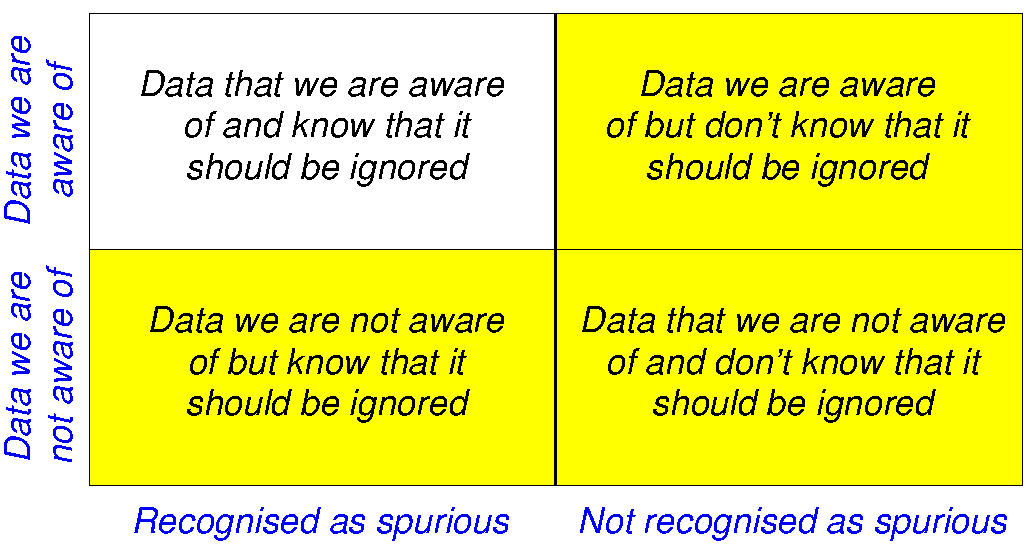
\includegraphics[width=\textwidth/2]{images/dazzleknowns.pdf}
  \caption{Dazzle data varieties}
  \label{fig:dazzle}
\end{figure}

\clearpage
\subsubsection{Dazzle Data Examples}

\paragraph{Data We Are Aware Of --- Recognised as Spurious}\index{Dazzle Data!Data We Know are Spurious or Unneeded}
Repeated false positive alerts (e.g. from faulty sensors or alarms). These tend to be annoying irritants rather than safety issues, however they can lead to alarms being permanently switched off, masking true problems. An example from everyday life might be removing the battery from a badly place smoke alarm in a kitchen which repeatedly sounds when the toaster is used.

\paragraph{Data We Are Aware Of --- Not Recognised as Spurious}\index{Dazzle Data!Data We Don't Know are Spurious or Unneeded}
Electromagnetic interference (EMI) affecting transmitted data is a good example of this case; we know it exists as a possibility but don't know how it might affect data in a system or a communications path, and this could be in different ways at different times or days.

\paragraph{Data We Are Not Aware Of --- Recognised as Spurious}\index{Dazzle Data!Data We Know are Spurious or Unneeded}
In many cases we do not know what changes or corruptions may affect the data, but we have strong correction mechanisms to cope with the problems regardless. A good example is data stores on a spacecraft which have redundancy and error correcting codes built-in and so can deal with the majority of corruptions caused by cosmic rays.

\paragraph{Data We Are Not Aware Of --- Not Recognised as Spurious}\index{Dazzle Data!Data We Don't Know are Spurious or Unneeded}
An example of this is where data is mistakenly added to a machine learning training data\index{Machine Learning Data} set resulting in bizarre and possibly hazardous behaviours of the system using it (e.g. an autonomous road vehicle). It is paramount that data used for such image recognition systems filters and excludes potentially dangerous extraneous data arising from unanticipated situations 

\subsubsection{Dazzle Data Varieties\index{Dazzle Data} and Safety Examples}
In his book, David Hand introduces a taxonomy of fifteen varieties of Dark Data\index{Dark Data}. This section discuses each form of Dazzle Data and considers it from a systems and safety assurance perspective.
Some of the varieties are the same as Dark Data\index{Dark Data}, but some are very different.

\paragraph{Data We Know are Superfluous or Unneeded: ``Known Extras''}\index{Dazzle Data!Data We Know are Spurious or Unneeded|textbf}
\label{bkm:dazzledata:case1}

This case is very common in systems where an interface\index{Interface!Flooding} may be flooded with unsolicited messages.
It is also common in  safety justifications\index{Justification, Safety} where assurance information may be padded out with extra, irrelevant information that can mask the underlying safety argument (which may or may not be intentional).
It can be a serious problem in large, complex safety documents or detailed safety analyses.
Luckily, in this case, the data is recognised as superfluous and can be ignored.
Common examples include:
\begin{itemize}
    \item Mailboxes filled with spam mail, preventing important messages being read
    \item Repeated stall warnings when the aircraft is under control
    \item Assurance information in a safety case is included for components which are not part of the solution in use at that site or situation
    \item Assurance information about old or legacy components is included but these are now not in service
    \item Machine learning training data\index{Machine Learning Data} contains many cases which are duplicates or very closely related, so adding nothing to the learned behaviour but making the set hard to deal with
\end{itemize}
This case can be mitigated\index{Mitigation} in several ways, including careful filtering, review, use of concise  notations (such as Goal Structuring Notation) to extract the essence, and periodic audits and cleans. 

\paragraph{Data We Don’t Know Are Unneeded or Spurious: ``Unknown Extras''}\index{Dazzle Data!Data We Don't Know are Spurious or Unneeded|textbf}
This is the most serious and far-reaching case, where the additional data is not recognised as unneeded and may be processed, analysed or be left in place when it should be removed. Some examples are:
\begin{itemize}
\item Legacy code in software\index{Software!Legacy} where nobody understands its function, or how it relates to the current code and so is reluctant to remove it. The Ariane 4 Inertial Reference function left in place in the Ariane 501 launch disaster might be such a case. Note that code whose function is known would be under the first case, discussed in \ref{bkm:dazzledata:case1}
    \item Parts of the safety case or safety argument are supplied separately (e.g. by a subcontractor or 3rd party) and they are obscure. In this case it will not be known which parts are relevant to the particular situation. Some information may be irrelevant or worse, misleading.
    \item Machine learning training data\index{Machine Learning Data} containing too many outliers, which are not recognised as such
\end{itemize}

In many cases the extra data may be discovered after some time, and it is incumbent on the organisation involved to analyse the impact of the complete set of data which may have been used over the time period, including subsequent decisions and actions. The effect of spurious data should not be underestimated, as it may have masked, prevented or distorted the intended use of the nominal data for some time. This case can fundamentally change the safety picture and is probably in the highest safety risk category.

Data found to be erroneous (i.e. it should not ever have been in the system or in the safety argument) is a problem. The following options show possible approaches to handling this data:
\begin{enumerate}[label=\color{dsiwgAccentColour}\roman*)]
    \item Delete the erroneous data
    \item Accept the erroneous data, i.e. continue using it
    \item Report that the data was erroneous but take no further action 
    \item Establish under what circumstances and situations the erroneous data would have had an effect
    \item Perform a full impact analysis on the effects of the erroneous data and then act according to the results
\end{enumerate}

\paragraph{Data Obscuration: Missing What Matters}\index{Dazzle Data!Data Obscuration}
This is where the meaning of the overall data set becomes obscured due to the extra unnecessary data. Examples might be:
\begin{itemize}
    \item Measuring the wrong things due to excessive noise or too much data to deal with
    \item Processing involving sampling only picks bad data elements
    \item Being too close to the data, i.e. the ``wood for the trees''. This is when the extra data masks the overall issue with the data, e.g. a slow trend or bias hidden by large local variations.
\end{itemize}

Mitigations\index{Mitigation} include review, statistical checks and ``taking a step back'' to look at the bigger picture.
\paragraph{Data Masking in Specific Cases}\index{Dazzle Data!Data Masking in Specific Cases}
This is where the extra data specifically masks, obscures or hides particular data elements (but not all). A particularly nasty case of this is where filters are put in place to remove unwanted data values, but those filters actually remove less (or more) than they should (i.e. don’t remove all unwanted cases or remove valid values as well). Some examples might be:
\begin{itemize}
    \item The number of successful test runs vastly outweighs failed runs and so the failures are not investigated
    \item Incorrect filtering of the data, leaving in some cases that should have been excluded
\end{itemize}

Mitigations\index{Mitigation} include use of review and \index{Completeness!Checks}completeness checks. Note that over-aggressive filtering would create cases of Dark Data\index{Dark Data}.
\paragraph{Masquerade or Fraudulent Data}\index{Dazzle Data!Masquerade or Fraudulent Data}
This is where data has been constructed to fool the system consuming it, hiding, overlaying or replacing the correct data. Often this will be malicious and should be filtered or rejected by the target system, but of course may not be. 
\begin{itemize}
    \item Intentional fraud
    \item Some security attacks
\end{itemize}

Mitigations\index{Mitigation} include audit, blockchain, monitoring, intelligent profiling of data and detection of changes.

\paragraph{Incorrect Definitions of Data}\index{Dazzle Data!Incorrect Definitions of Data}
This is considered a common case for systems exchanging data with external systems, where they may duplicate, translate or incorrectly send multiple messages. They may be time-separated, for instance if communications are lost and then regained, leading to confusion.
\begin{itemize}
    \item Data sent in the wrong rate or units (e.g. every millisecond rather than second)
    \item Data given for the wrong range or duration (e.g. for a month rather than a day
    \item Data sent for the wrong domain or scale (e.g. national values rather than regional)
    \item Text messages re-sent to a mobile phone when coverage restored
\end{itemize}

Mitigations\index{Mitigation} include making sure interface\index{Interface!Specification} specifications are clear and ambiguous, rejecting incorrect size or scale data sets, keeping a list of known changes / incompatibilities and documenting the changes or fixes that have to be applied to make the data usable or consistent.

\paragraph{Summaries of Data}\index{Dazzle Data!Summaries of Data}
Spurious data can affect summaries in a significant way if composite values are calculated, e.g.
\begin{itemize}
    \item Calculations of averages or other statistics affected by duplicates
    \item Spurious outliers can lead to over fitting when analysing data trends
\end{itemize}

Mitigations\index{Mitigation} include audit and assessing what extra data could cause (i.e. performing sensitivity analysis) and establishing what decisions might be made erroneously due to certain data values being present.	

\paragraph{Information Asymmetry}\index{Dazzle Data!Information Asymmetry}
This is common where there are multiple stores or sources of the same data. If one has erroneous duplicate values (i.e. many null values used for padding) then comparisons between them may fail.
\begin{itemize}
    \item Multiple / backup databases where they are not kept in sync
    \item Issues of divergence of data across multiple sources.
\end{itemize}

Comparisons, reviews and data audits may help in these cases. In general the issue of divergence across multiple data sources needs to be recognised and addressed in an automated way.

\paragraph{Intentionally Dazzled Data}\index{Dazzle Data!Intentionally Dazzled Data}
This might happen in a secure context where key data is effectively ``camouflaged'' by hiding within large data items (e.g. images) or the use of large amounts of apparently routine data to mask the secure data.
\begin{itemize}
    \item Defence, security and government sectors where data is purposefully hidden 
    \item An organisation may provide copious amounts of safety case collateral to hide a weak safety case
\end{itemize}
\paragraph{Extrapolating Beyond Your Data}\index{Dazzle Data!Extrapolating Beyond your Data}
Machine learning systems have to cope with values outside of their training data\index{Machine Learning Data}, but the outcomes may be unexpected if the training data contains many spurious values:
\begin{itemize}
    \item Bizarre results from recognition / detection systems due to out of range values
    \item Image components mislabelled leading to strange results
\end{itemize}

Mitigations\index{Mitigation} include checking of the values that are used in training, analysis of outliers and repeats, deletion of duplicates and use of machine learning validation data\index{Machine Learning Data} containing edge/corner cases and boundary cases.

\paragraph{A Note on Sensors}
Sensors can degrade and fail over time, especially in harsh environments such as automotive, marine or aviation. In such cases sensors may feed erroneous or additional data into systems (e.g. if an out of normal range situation is detected), leading to misleading processing or false alarms. The \index{Boeing 737}Boeing 737 MAX~8 accidents might fall into this category as the angle-of-attack sensor erroneously generated high values, and certainly the systems/processing which passed on the values created spurious data. Some examples are:
\begin{itemize}
    \item Faulty sensors
    \item Multiple sensors that do not have their values properly combined
    \item Sampling techniques which generate additional data
    \item Interval polling interval can lead to misleading readings
    \item Data fusion can be impacted if multiple sensor values are combined
\end{itemize}

Mitigations\index{Mitigation} include independent monitoring of sensors and regular maintenance, calibration or replacement of hardware. Their interfaces\index{Interface!Sensor} need to be able to detect any problems and report faults. In particularly critical applications, it may be necessary to minimise the potential for common mode failures by using disparate technologies, or at least sensors from different manufacturers.

An example may be found in\index{Qantas}
\href{https://en.wikipedia.org/wiki/Qantas\_Flight\_72}{https://en.wikipedia.org/wiki/Qantas\_Flight\_72}
where:
\begin{quotation}
  \dots the \glsxtrshort{cpu}\footnote{\Glsxtrlong{cpu}} of the \glsxtrshort{adiru}\index{ADIRU}\footnote{\Glsxtrlong{adiru}} corrupted the \glsxtrshort{aoa}\footnote{\Glsxtrlong{aoa}} data. The exact nature of the corruption was that the \glsxtrshort{adiru} \glsxtrshort{cpu} erroneously re-labelled the altitude data word so that the binary data that represented 37,012 (the altitude at the time of the incident) would represent an angle of attack of 50.625 degrees. The \glsxtrshort{fcpc}\footnote{\Glsxtrlong{fcpc}} then processed the erroneously high \gls{aoa} data, triggering the high-\gls{aoa} protection mode, which sent a command to the electrical flight control system (EFCS) to pitch the nose down.
  
  The \glsxtrshort{fcpc} algorithm was very effective, but it could not correctly manage a scenario where there were multiple spikes in either \gls{aoa} 1 or \gls{aoa} 2 that were 1.2 seconds apart --- i.e., if the 1.2-second period of use of the memorised value happened to end while another spike was happening.
  \end{quotation}
\subsubsection{Summary of Dazzle Data}
Dazzle Data is a very useful way of thinking about data problems and solutions.
It is important to always think of the bigger picture,
considering what information is superfluous and may be distorting or masking the real picture:
\begin{itemize}
    \item What might be hidden intentionally or otherwise due to the extra values?
    \item Could the extra items cause any safety problems, e.g. change a numerical calculation?
    \item How would a system cope if it received data it was not expecting?
    \item How do you characterise the nature of unexpected data so as to ensure it can be handled if it does occur?
    \item Can you present your results / outputs in a way that shows the extra data?
\end{itemize}
%
% Comparison table
%
\subsection{Links between Dark Data / Dazzle Data and Data Properties}
\index{Dazzle Data!Comparison with Dark Data}
\index{Dark Data!Comparison with Dazzle Data}
Fundamentally, Dark Data is data that is not available, but nevertheless is important, and indeed, in some cases, more important than the data that is available.

Similarly, Dazzle Data refers to spurious, superfluous or unexpected data that masks and confuses the picture and
can reduce your ability to see details, and indeed the whole picture --- a bit like noise or camouflage.

The opposite attributes of dark data and dazzle data might be termed Brightness and Clarity respectively. These are potential new properties or meta-properties of data.

\autoref{tab:DarkDazzleComparison} illustrates the properties which can be affected by Dark Data and Dazzle Data issues.

\begin{longtable}{|L{\dsiwgColumnWidth{0.17}}|L{\dsiwgColumnWidth{0.17}}|C{\dsiwgColumnWidth{0.17}}|C{\dsiwgColumnWidth{0.17}}|L{\dsiwgColumnWidth{0.32}}|}
  \caption{Data Properties Affected by Dark Data and / or  Dazzle Data Issues}
  \label{tab:DarkDazzleComparison}
  \\\hline\TableHeadColour{Data Property} & \TableHeadColour{Explanation} & \TableHeadColour{Dark Data --- missing data} & \TableHeadColour{Dazzle data --- obscuring data} & \TableHeadColour{Notes}\\\hline
  \endfirsthead
  \caption[]{Data Properties Affected by Dark Data and / or  Dazzle Data Issues (continued)}
  \\\hline\TableHeadColour{Data Property} & \TableHeadColour{Explanation} & \TableHeadColour{Dark Data --- missing data} & \TableHeadColour{Dazzle data --- obscuring data} & \TableHeadColour{Notes}\\\hline
  \endhead
  \multicolumn{5}{r}{\sl Continued on next page}
  \endfoot\endlastfoot
  %
  Integrity (I) & The data is correct, true and unaltered & \tick & \tick &
  E.g., Corruptions to a database could change the original values so the original data is lost, or hide or mask values such as by inserting End-of-File markers\\
  \hline
  %
  Completeness (C) & The data has nothing missing or lost & \tick & - &
  If data is lost then it is usually unknown and hence dark. However use of parity, CRCs and digital signatures may be able to detect the loss and, in some cases, fill in the missing data.\\
  \hline
  %
  Consistency (N) & The data adheres to a common world view (e.g., units) & - & - &\\
  \hline
  %
  Continuity (Y) & The data is continuous and regular without gaps or breaks & \tick & - &
  Gaps or breaks in a data stream would be dark --- the missing values are unknown.
  Methods may be available to mitigate if detected, e.g., interpolation.\\
  \hline
  %
  Format (O) & The data is represented in a way which is readable by those that need to use it & \tick & \tick &
  If data is not in the correct format then it may not be usable so becomes dark. If lots of data is in the wrong format it may obscure other (good) data, and hence can dazzle.\\
  \hline
  %
  \Gls{accuracy} (A) & The data has sufficient detail for its intended use & \tick & - &
  If the data has lost detail (e.g., due to sensor sampling or representation) then this is a dark case.\\
  \hline
  %
  Resolution (R) & The smallest difference between two adjacent values that can be represented
  in a data storage, display or transfer system & \tick & \tick &
  If the system cannot distinguish between different data values that actually are different, then data could become hidden or lost and hence dark. If the data is masked then it may also be a case of dazzle data.\\
  \hline
  %
  Traceability (T) & The data can be linked back to its source or derivation & \tick & - &
  If traceability is lost then the data effectively becomes darker as its origins and derivation are lost, and may not be able to be used.\\
  \hline
  %
  Timeliness (M) & The data is as up to date as required & \tick & \tick &
  If data is not, or thought to be not, up to date then it may be rejected and hence become dark data. But clocks can become out of sync across different systems leading to erroneous rejection so the timestamps may then be thought of as dazzling the system.\\
  \hline
  %
  Verifiability (V) & The data can be checked and its properties demonstrated to be correct & \tick & - &
  If data can’t be checked then it may be rejected (and become dark), even if it is valid.\\
  \hline
  %
  Availability (L) & The data is accessible and usable when an authorised entity demands access & \tick & - &
  If data is not available as required then it is dark (whether it exists or not).\\
  \hline
  %
  Fidelity / Representation (F) & How well the data maps to the real-world entity it is trying to model &
  - & - &\\
  \hline
  %
  Priority (P) & The data is presented / transmitted / made available in the order required &
  \tick & \tick &
  If data is not prioritised to be available when needed it is effectively dark. This could be because other data is taking precedence so could be a dazzle case.\\
  \hline
  %
  Sequencing (Q) & The data is preserved in the order required &
  \tick & \tick &
  If data is not sequenced as needed it may be rejected or ignored and then is effectively dark. Other data which is out of order or sequence may cause the whole message, set or file to be rejected – a dazzle case.\\
  \hline
  %
  Intended Destination / Usage (U) & The data is only sent to those that should have access to it &
  \tick & - &
  If data is not sent to the correct destination it may be a dark data situation as it is effectively missing.\\
  \hline
  %
  Accessibility (B) & The data is visible only to those that should see it &
  - & \tick &
  If data is more widely visible or distributed than intended it could cause a dazzle situation due to e.g. bandwidth issues.\\
  \hline
  %
  Suppression (S) & The data is intended never to be used again &
  - & \tick &
  If data re-emerges after it should have been deleted it could cause all sorts of dazzle-related problems.\\
  \hline
  %
  History (H) & The data has an audit trail of changes &
  \tick & - &
  If the audit trail is lost then the data is darkened as its origins and derivation could be important.\\
  \hline
  %
  Lifetime (E) & When does the safety-related data expire &
  \tick & \tick &
  If the lifetime is erroneously early than the data is lost --- a dark data problem. Conversely if the lifetime is too long it is potentially a dazzle situation.\\
  \hline
  %
  Disposability / Deletability (D) & The data can be permanently removed when required &
  - & \tick &
  If the data cannot be removed it is potentially a dazzle situation, as it may obscure the real or current data.\\
  \hline
  %
  Goldilocks (G) & The data is just the right size — not too much and not too little &
  \tick & \tick &
  Too little data may be a dark data case and too much data to deal with is a dazzle case.\\
  \hline
  %
  Analysability (Z) & The data is of a suitable size, type and representation (including any metadata) to enable it be usefully analysed &
  \tick & \tick &
  If the data can’t be analysed it may not be able to be used causing a dark data issue. If there is too much of it or it is obscured (e.g., by noise on a comms line) then it is a dazzle case.\\
  \hline
  %
  Explainability (X) & The data can be meaningfully explained to those who need to understand it by a suitable mechanism &
  \tick & \tick &
  If the data can’t be explained it may not be able to be used causing a dark data issue. If there is too much of it or suitable management and analysis tools are not available then it is potentially both cases.\\
  \hline
  %
\end{longtable}

%  %================================================================================
%       Safety Critical Systems Club - Data Safety Initiative Working Group
%================================================================================
%                       DDDD    SSSS  IIIII  W   W   GGGG
%                       D   D  S        I    W   W  G   
%                       D   D   SSS     I    W W W  G  GG
%                       D   D      S    I    WW WW  G   G
%                       DDDD   SSSS   IIIII  W   W   GGG
%================================================================================
%               Data Safety Guidance Document - LaTeX Source File
%================================================================================
%
% Description:
%   Appendix regarding Dazzle / distracting / disruptive data
%   Originally typeset from draft 0.5 and later updated to 0.7
%================================================================================
\section{Dazzle Data and Safety (Informative)}\index{Dazzle Data|textbf}\index{Data!Dazzle|see{Dazzle Data}} \label{bkm:dazzledata}
%
%\dsiwgSectionQuote{A ship in a port is safe, but that's not what ships are built for}{Grace Hopper}

%\dsiwgSectionQuote{Don't fix the blame, fix the problem}{Keith Pennington}

\dsiwgSectionQuote{Camouflage is a game we all like to play, but our secrets are as surely revealed by what we want to seem to be as by what we want to conceal}{Russell Lynes}

\subsection{Introduction}
This appendix outlines some of the safety implications arising from the issues identified by
``Dazzle Data'' in contrast to ``Dark Data''\index{Dark Data} presented in David Hand's book:
``Dark Data: Why What You Don't Know Matters'' \cite{citation:darkdata:hand}
and website \cite{citation:darkdata:website}.
Dark Data\index{Dark Data} relates to data that is not available but nevertheless is important.

``Dazzle Data'' refers to spurious, superfluous or unexpected data that masks and confuses the picture and can reduce your ability to see details, and indeed the whole picture -- a bit like noise or camouflage.

\begin{quote}
  It is data you don't want, didn't ask for, arrives more frequently than expected, is redundant, or data that arrives at an unexpected or inconvenient time or in the wrong format or sequence, so requiring extra resources to deal with\dots
\end{quote}

At first sight it might be thought this is just an annoyance rather than a problem,
however Dazzle Data can mask, distort or prevent usage of the real or desired data.
It can hide the true picture as in ``wood for the trees'' and in the worst case create real problems. 

Some examples of such false positive alerts that cause real alerts to be ignored are:
\begin{itemize}
  \item The classic case of ``Crying Wolf''.
  \item Denial of Service Attack, when servers can be blocked with useless requests that cannot be distinguished from the real requests.
\end{itemize}

Data which is truly spurious and believable (e.g. generated by extensive electrical noise, or fabricated to mask a fraud) may be accepted as valid data, leading to potentially hazardous results. 

Varieties of Dazzle Data may be identified\index{Dazzle Data} in the same grid manner as Dark Data\index{Dark Data}, as shown in \autoref{fig:dazzle}, where the yellow areas indicate potential dazzle data.

\begin{figure}[htbp]
  \centering
  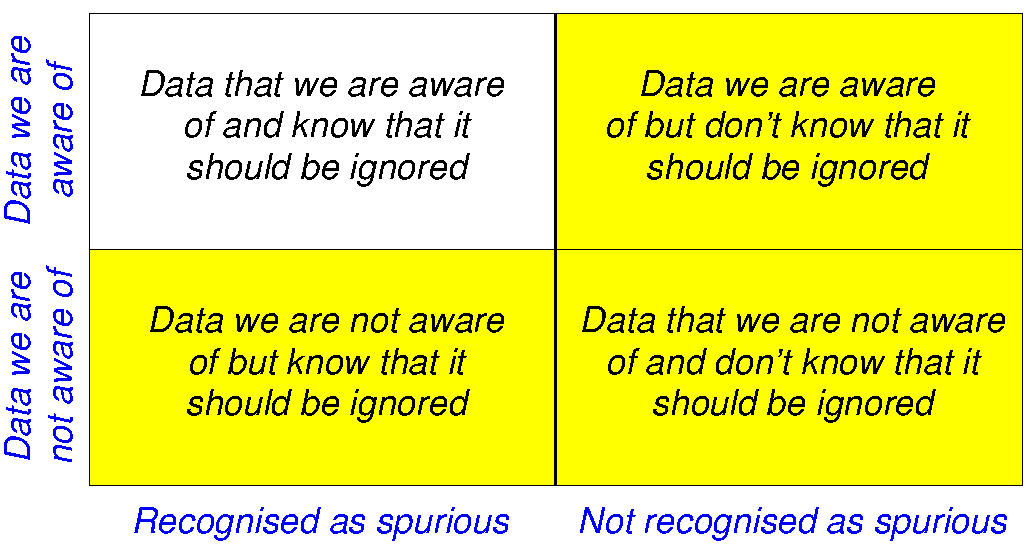
\includegraphics[width=\textwidth/2]{images/dazzleknowns.pdf}
  \caption{Dazzle data varieties}
  \label{fig:dazzle}
\end{figure}

\clearpage
\subsection{Dazzle Data Examples}

\subsubsection{Data We Are Aware Of -- Recognized as Spurious}\index{Dazzle Data!Data We Know are Spurious or Unneeded}
Repeated false positive alerts (e.g. from faulty sensors or alarms). These tend to be annoying irritants rather than safety issues, however they can lead to alarms being permanently switched off, masking true problems. An example from everyday life might be removing the battery from a badly place smoke alarm in a kitchen which repeatedly sounds when the toaster is used.

\subsubsection{Data We Are Aware Of -- Not Recognized as Spurious}\index{Dazzle Data!Data We Don't Know are Spurious or Unneeded}
Electromagnetic interference (EMI) affecting transmitted data is a good example of this case; we know it exists as a possibility but don't know how it might affect data in a system or a communications path, and this could be in different ways at different times or days.

\subsubsection{Data We Are Not Aware Of -- Recognized as Spurious}\index{Dazzle Data!Data We Know are Spurious or Unneeded}
In many cases we do not know what changes or corruptions may affect the data, but we have strong correction mechanisms to cope with the problems regardless. A good example is data stores on a spacecraft which have redundancy and error correcting codes built-in and so can deal with the majority of corruptions caused by cosmic rays.

\subsubsection{Data We Are Not Aware Of -- Not Recognized as Spurious}\index{Dazzle Data!Data We Don't Know are Spurious or Unneeded}
An example of this is where data is mistakenly added to a machine learning training data\index{Machine Learning Data} set resulting in bizarre and possibly hazardous behaviours of the system using it (e.g. an autonomous road vehicle). It is paramount that data used for such image recognition systems filters and excludes potentially dangerous extraneous data arising from unanticipated situations 

\subsection{Dazzle Data Varieties\index{Dazzle Data} and Safety Examples}
In his book, David Hand introduces a taxonomy of fifteen varieties of Dark Data\index{Dark Data}. This section discuses each form of Dazzle Data and considers it from a systems and safety assurance perspective.
Some of the varieties are the same as Dark Data\index{Dark Data}, but some are very different.

\subsubsection{Data We Know are Superfluous or Unneeded: ``Known Extras''}\index{Dazzle Data!Data We Know are Spurious or Unneeded|textbf}
\label{bkm:dazzledata:case1}

This case is very common in systems where an interface\index{Interface!Flooding} may be flooded with unsolicited messages.
It is also common in  safety justifications\index{Justification, Safety} where assurance information may be padded out with extra, irrelevant information that can mask the underlying safety argument (which may or may not be intentional).
It can be a serious problem in large, complex safety documents or detailed safety analyses.
Luckily, in this case, the data is recognized as superfluous and can be ignored.
Common examples include:
\begin{itemize}
    \item Mailboxes filled with spam mail, preventing important messages being read
    \item Repeated stall warnings when the aircraft is under control
    \item Assurance information in a safety case is included for components which are not part of the solution in use at that site or situation
    \item Assurance information about old or legacy components is included but these are now not in service
    \item Machine learning training data\index{Machine Learning Data} contains many cases which are duplicates or very closely related, so adding nothing to the learned behaviour but making the set hard to deal with
\end{itemize}
This case can be mitigated\index{Mitigation} in several ways, including careful filtering, review, use of concise  notations (such as Goal Structuring Notation) to extract the essence, and periodic audits and cleans. 

\subsubsection{Data We Don’t Know Are Unneeded or Spurious: ``Unknown Extras''}\index{Dazzle Data!Data We Don't Know are Spurious or Unneeded|textbf}
This is the most serious and far-reaching case, where the additional data is not recognized as unneeded and may be processed, analysed or be left in place when it should be removed. Some examples are:
\begin{itemize}
\item Legacy code in software\index{Software!Legacy} where nobody understands its function, or how it relates to the current code and so is reluctant to remove it. The Ariane 4 Inertial Reference function left in place in the Ariane 501 launch disaster might be such a case. Note that code whose function is known would be under the first case, discussed in \ref{bkm:dazzledata:case1}
    \item Parts of the safety case or safety argument are supplied separately (e.g. by a subcontractor or 3rd party) and they are obscure. In this case it will not be known which parts are relevant to the particular situation. Some information may be irrelevant or worse, misleading.
    \item Machine learning training data\index{Machine Learning Data} containing too many outliers, which are not recognized as such
\end{itemize}

In many cases the extra data may be discovered after some time, and it is incumbent on the organization involved to analyse the impact of the complete set of data which may have been used over the time period, including subsequent decisions and actions. The effect of spurious data should not be underestimated, as it may have masked, prevented or distorted the intended use of the nominal data for some time. This case can fundamentally change the safety picture and is probably in the highest safety risk category.

Data found to be erroneous (i.e. it should not ever have been in the system or in the safety argument) is a problem. The following options show possible approaches to handling this data:
\begin{enumerate}[label=\color{dsiwgAccentColour}\roman*)]
    \item Delete the erroneous data
    \item Accept the erroneous data, i.e. continue using it
    \item Report that the data was erroneous but take no further action 
    \item Establish under what circumstances and situations the erroneous data would have had an effect
    \item Perform a full impact analysis on the effects of the erroneous data and then act according to the results
\end{enumerate}

\subsubsection{Data Obscuration: Missing What Matters}\index{Dazzle Data!Data Obscuration}
This is where the meaning of the overall data set becomes obscured due to the extra unnecessary data. Examples might be:
\begin{itemize}
    \item Measuring the wrong things due to excessive noise or too much data to deal with
    \item Processing involving sampling only picks bad data elements
    \item Being too close to the data, i.e. the ``wood for the trees''. This is when the extra data masks the overall issue with the data, e.g. a slow trend or bias hidden by large local variations.
\end{itemize}

Mitigations\index{Mitigation} include review, statistical checks and ``taking a step back'' to look at the bigger picture.
\subsubsection{Data Masking in Specific Cases}\index{Dazzle Data!Data Masking in Specific Cases}
This is where the extra data specifically masks, obscures or hides particular data elements (but not all). A particularly nasty case of this is where filters are put in place to remove unwanted data values, but those filters actually remove less (or more) than they should (i.e. don’t remove all unwanted cases or remove valid values as well). Some examples might be:
\begin{itemize}
    \item The number of successful test runs vastly outweighs failed runs and so the failures are not investigated
    \item Incorrect filtering of the data, leaving in some cases that should have been excluded
\end{itemize}

Mitigations\index{Mitigation} include use of review and \index{Completeness!Checks}completeness checks. Note that over-aggressive filtering would create cases of Dark Data\index{Dark Data}.
\subsubsection{Masquerade or Fraudulent Data}\index{Dazzle Data!Masquerade or Fraudulent Data}
This is where data has been constructed to fool the system consuming it, hiding, overlaying or replacing the correct data. Often this will be malicious and should be filtered or rejected by the target system, but of course may not be. 
\begin{itemize}
    \item Intentional fraud
    \item Some security attacks
\end{itemize}

Mitigations\index{Mitigation} include audit, blockchain, monitoring, intelligent profiling of data and detection of changes.

\subsubsection{Incorrect Definitions of Data}\index{Dazzle Data!Incorrect Definitions of Data}
This is considered a common case for systems exchanging data with external systems, where they may duplicate, translate or incorrectly send multiple messages. They may be time-separated, for instance if communications are lost and then regained, leading to confusion.
\begin{itemize}
    \item Data sent in the wrong rate or units (e.g. every millisecond rather than second)
    \item Data given for the wrong range or duration (e.g. for a month rather than a day
    \item Data sent for the wrong domain or scale (e.g. national values rather than regional)
    \item Text messages re-sent to a mobile phone when coverage restored
\end{itemize}

Mitigations\index{Mitigation} include making sure interface\index{Interface!Specification} specifications are clear and ambiguous, rejecting incorrect size or scale data sets, keeping a list of known changes / incompatibilities and documenting the changes or fixes that have to be applied to make the data usable or consistent.

\subsubsection{Summaries of Data}\index{Dazzle Data!Summaries of Data}
Spurious data can affect summaries in a significant way if composite values are calculated, e.g.
\begin{itemize}
    \item Calculations of averages or other statistics affected by duplicates
    \item Spurious outliers can lead to overfitting when analysing data trends
\end{itemize}

Mitigations\index{Mitigation} include audit and assessing what extra data could cause (i.e. performing sensitivity analysis) and establishing what decisions might be made erroneously due to certain data values being present.	

\subsubsection{Information Asymmetry}\index{Dazzle Data!Information Asymmetry}
This is common where there are multiple stores or sources of the same data. If one has erroneous duplicate values (i.e. many null values used for padding) then comparisons between them may fail.
\begin{itemize}
    \item Multiple / backup databases where they are not kept in sync
    \item Issues of divergence of data across multiple sources.
\end{itemize}

Comparisons, reviews and data audits may help in these cases. In general the issue of divergence across multiple data sources needs to be recognized and addressed in an automated way.

\subsubsection{Intentionally Dazzled Data}\index{Dazzle Data!Intentionally Dazzled Data}
This might happen in a secure context where key data is effectively ``camouflaged'' by hiding within large data items (e.g. images) or the use of large amounts of apparently routine data to mask the secure data.
\begin{itemize}
    \item Defence, security and government sectors where data is purposefully hidden 
    \item An organization may provide copious amounts of safety case collateral to hide a weak safety case
\end{itemize}
\subsubsection{Extrapolating Beyond Your Data}\index{Dazzle Data!Extrapolating Beyond your Data}
Machine learning systems have to cope with values outside of their training data\index{Machine Learning Data}, but the outcomes may be unexpected if the training data contains many spurious values:
\begin{itemize}
    \item Bizarre results from recognition / detection systems due to out of range values
    \item Image components mislabelled leading to strange results
\end{itemize}

Mitigations\index{Mitigation} include checking of the values that are used in training, analysis of outliers and repeats, deletion of duplicates and use of machine learning validation data\index{Machine Learning Data} containing edge/corner cases and boundary cases.

\paragraph{A Note on Sensors}
Sensors can degrade and fail over time, especially in harsh environments such as automotive, marine or aviation. In such cases sensors may feed erroneous or additional data into systems (e.g. if an out of normal range situation is detected), leading to misleading processing or false alarms. The \index{Boeing 737}Boeing 737 MAX~8 accidents might fall into this category as the angle-of-attack sensor erroneously generated high values, and certainly the systems/processing which passed on the values created spurious data. Some examples are:
\begin{itemize}
    \item Faulty sensors
    \item Multiple sensors that do not have their values properly combined
    \item Sampling techniques which generate additional data
    \item Interval polling interval can lead to misleading readings
    \item Data fusion can be impacted if multiple sensor values are combined
\end{itemize}

Mitigations\index{Mitigation} include independent monitoring of sensors and regular maintenance, calibration or replacement of hardware. Their interfaces\index{Interface!Sensor} need to be able to detect any problems and report faults. In particularly critical applications, it may be necessary to minimise the potential for common mode failures by using disparate technologies, or at least sensors from different manufacturers.

An example may be found in\index{Qantas}
\href{https://en.wikipedia.org/wiki/Qantas\_Flight\_72}{https://en.wikipedia.org/wiki/Qantas\_Flight\_72}
where:
\begin{quotation}
  \dots the \acrshort{cpu}\footnote{\acrlong{cpu}} of the \acrshort{adiru}\index{ADIRU}\footnote{\acrlong{adiru}} corrupted the \acrfull{aoa} data. The exact nature of the corruption was that the \acrshort{adiru} \acrshort{cpu} erroneously re-labelled the altitude data word so that the binary data that represented 37,012 (the altitude at the time of the incident) would represent an angle of attack of 50.625 degrees. The \acrshort{fcpc}\footnote{\acrlong{fcpc}} then processed the erroneously high \gls{aoa} data, triggering the high-\gls{aoa} protection mode, which sent a command to the electrical flight control system (EFCS) to pitch the nose down.
  
  The \acrshort{fcpc} algorithm was very effective, but it could not correctly manage a scenario where there were multiple spikes in either \gls{aoa} 1 or \gls{aoa} 2 that were 1.2 seconds apart -- i.e., if the 1.2-second period of use of the memorised value happened to end while another spike was happening.
  \end{quotation}

\subsection{Summary}
Dazzle Data is a very useful way of thinking about data problems and solutions.
It is important to always think of the bigger picture,
considering what information is superfluous and may be distorting or masking the real picture:
\begin{itemize}
    \item What might be hidden intentionally or otherwise due to the extra values?
    \item Could the extra items cause any safety problems, e.g. change a numerical calculation?
    \item How would a system cope if it received data it was not expecting?
    \item How do you characterise the nature of unexpected data so as to ensure it can be handled if it does occur?
    \item Can you present your results / outputs in a way that shows the extra data?
\end{itemize}

Fundamentally, Dark Data is data that is not available, but nevertheless is important, and indeed, in some cases, more important than the data that is available.

Similarly, Dazzle Data refers to spurious, superfluous or unexpected data that masks and confuses the picture and
can reduce your ability to see details, and indeed the whole picture -- a bit like noise or camouflage.

The opposite attributes of dark data and dazzle data might be termed Brightness and Clarity respectively. These are potential new properties or meta-properties of data.

\begin{longtable}{|L{\dsiwgColumnWidth{0.17}}|L{\dsiwgColumnWidth{0.17}}|C{\dsiwgColumnWidth{0.17}}|C{\dsiwgColumnWidth{0.17}}|L{\dsiwgColumnWidth{0.32}}|}
  \caption{A comparison of Dark and Dazzle data properties}
  \label{tab:DarkDazzleComparison}
  \\\hline\TableHeadColour{Data Property} & \TableHeadColour{Explanation} & \TableHeadColour{Dark Data -- missing data} & \TableHeadColour{Dazzle data -- obscuring data} & \TableHeadColour{Notes}\\\hline
  \endfirsthead
  \caption[]{A comparison of Dark and Dazzle data properties (continued)}
  \\\hline\TableHeadColour{Data Property} & \TableHeadColour{Explanation} & \TableHeadColour{Dark Data -- missing data} & \TableHeadColour{Dazzle data -- obscuring data} & \TableHeadColour{Notes}\\\hline
  \endhead
  \multicolumn{5}{r}{\sl Continued on next page}
  \endfoot\endlastfoot
  %
  Integrity (I) & The data is correct, true and unaltered & \tick & \tick &
  E.g., Corruptions to a database could change the original values so the original data is lost, or hide or mask values such as by inserting End-of-File markers\\
  \hline
  %
  Completeness (C) & The data has nothing missing or lost & \tick & - &
  If data is lost then it is usually unknown and hence dark. However use of parity, CRCs and digital signatures may be able to detect the loss and, in some cases, fill in the missing data.\\
  \hline
  %
  Consistency (N) & The data adheres to a common world view (e.g., units) & - & - &\\
  \hline
  %
  Continuity (Y) & The data is continuous and regular without gaps or breaks & \tick & - &
  Gaps or breaks in a data stream would be dark -- the missing values are unknown.
  Methods may be available to mitigate if detected, e.g., interpolation.\\
  \hline
  %
  Format (O) & The data is represented in a way which is readable by those that need to use it & \tick & \tick &
  If data is not in the correct format then it may not be usable so becomes dark. If lots of data is in the wrong format it may obscure other (good) data, and hence can dazzle.\\
  \hline
  %
  Accuracy (A) & The data has sufficient detail for its intended use & \tick & - &
  If the data has lost detail (e.g., due to sensor sampling or representation) then this is a dark case.\\
  \hline
  %
  Resolution (R) & The smallest difference between two adjacent values that can be represented
  in a data storage, display or transfer system & \tick & \tick &
  If the system cannot distinguish between different data values that actually are different, then data could become hidden or lost and hence dark. If the data is masked then it may also be a case of dazzle data.\\
  \hline
  %
  Traceability (T) & The data can be linked back to its source or derivation & \tick & - &
  If traceability is lost then the data effectively becomes darker as its origins and derivation are lost, and may not be able to be used.\\
  \hline
  %
  Timeliness (M) & The data is as up to date as required & \tick & \tick &
  If data is not, or thought to be not, up to date then it may be rejected and hence become dark data. But clocks can become out of sync across different systems leading to erroneous rejection so the timestamps may then be thought of as dazzling the system.\\
  \hline
  %
  Verifiability (V) & The data can be checked and its properties demonstrated to be correct & \tick & - &
  If data can’t be checked then it may be rejected (and become dark), even if it is valid.\\
  \hline
  %
  Availability (L) & The data is accessible and usable when an authorized entity demands access & \tick & - &
  If data is not available as required then it is dark (whether it exists or not).\\
  \hline
  %
  Fidelity / Representation (F) & How well the data maps to the real-world entity it is trying to model &
  - & - &\\
  \hline
  %
  Priority (P) & The data is presented / transmitted / made available in the order required &
  \tick & \tick &
  If data is not prioritised to be available when needed it is effectively dark. This could be because other data is taking precedence so could be a dazzle case.\\
  \hline
  %
  Sequencing (Q) & The data is preserved in the order required &
  \tick & \tick &
  If data is not sequenced as needed it may be rejected or ignored and then is effectively dark. Other data which is out of order or sequence may cause the whole message, set or file to be rejected – a dazzle case.\\
  \hline
  %
  Intended Destination / Usage (U) & The data is only sent to those that should have access to it &
  \tick & - &
  If data is not sent to the correct destination it may be a dark data situation as it is effectively missing.\\
  \hline
  %
  Accessibility (B) & The data is visible only to those that should see it &
  - & \tick &
  If data is more widely visible or distributed than intended it could cause a dazzle situation due to e.g. bandwidth issues.\\
  \hline
  %
  Suppression (S) & The data is intended never to be used again &
  - & \tick &
  If data re-emerges after it should have been deleted it could cause all sorts of dazzle-related problems.\\
  \hline
  %
  History (H) & The data has an audit trail of changes &
  \tick & - &
  If the audit trail is lost then the data is darkened as its origins and derivation could be important.\\
  \hline
  %
  Lifetime (E) & When does the safety-related data expire &
  \tick & \tick &
  If the lifetime is erroneously early than the data is lost -- a dark data problem. Conversely if the lifetime is too long it is potentially a dazzle situation.\\
  \hline
  %
  Disposability / Deletability (D) & The data can be permanently removed when required &
  - & \tick &
  If the data cannot be removed it is potentially a dazzle situation, as it may obscure the real or current data.\\
  \hline
  %
  Goldilocks (G) & The data is just the right size — not too much and not too little &
  \tick & \tick &
  Too little data may be a dark data case and too much data to deal with is a dazzle case.\\
  \hline
  %
  Analysability (Z) & The data is of a suitable size, type and representation (including any metadata) to enable it be usefully analysed &
  \tick & \tick &
  If the data can’t be analysed it may not be able to be used causing a dark data issue. If there is too much of it or it is obscured (e.g., by noise on a comms line) then it is a dazzle case.\\
  \hline
  %
  Explainability (X) & The data can be meaningfully explained to those who need to understand it by a suitable mechanism &
  \tick & \tick &
  If the data can’t be explained it may not be able to be used causing a dark data issue. If there is too much of it or suitable management and analysis tools are not available then it is potentially both cases.\\
  \hline
  %
\end{longtable}

  %================================================================================
%       Safety Critical Systems Club - Data Safety Initiative Working Group
%================================================================================
%                       DDDD    SSSS  IIIII  W   W   GGGG
%                       D   D  S        I    W   W  G   
%                       D   D   SSS     I    W W W  G  GG
%                       D   D      S    I    WW WW  G   G
%                       DDDD   SSSS   IIIII  W   W   GGG
%================================================================================
%               Data Safety Guidance Document - LaTeX Source File
%================================================================================
%
% Description:
%   Appendix regarding tool issues and seletion
%================================================================================
\section{Data Cygnology (Informative)}\index{Data Cygnology}\label{bkm:cygnology}
%
\dsiwgSectionQuote{Here be dragons}{Anon}

\subsection{Introduction}
The term “Black Swan” is used to describe an unpredictable event that is beyond what is normally expected of a situation and has potentially severe consequences.
Black Swan events were originally discussed in a financial context by Nassim Taleb in his 2004 book
\dsiwgTextIT{“Fooled By Randomness”} \cite{citation:cyg:RoleOfChance}
and further expanded to cover other topics in
\dsiwgTextIT{“The Black Swan: The Impact of the Highly Improbable”}
\cite{citation:cyg:BlackSwan}.
The term quickly became accepted, and Black Swan events are characterized by their extreme rarity, severe impact, and the widespread insistence they were obvious in hindsight. Taleb gave examples such as the rise of the Internet, the personal computer and financial crashes as “Black Swan” events, but the term can equally be applied to unexpected safety-related events such as the Boeing 737 MAX crashes of 2018 / 2019 \cite{citation:cyg:737Max}.

While Black Swans are events that are only obvious in hindsight, other types of event may be extremely rare and have severe impact but are predictable beforehand, for example pandemics.
Another example comes from the sun:  a Coronal Mass Ejection (CME) of such severity can be produced that it causes widespread life-threatening electromagnetic interference on Earth.
This type of event can be predicted to occur to some extent, and has happened before, for example the “Carrington Event” of 1859 \cite{citation:cyg:carrington}.
These rare events which have rapid escalation, but are somewhat predictable are termed “Dragon King” events.

There are several more event types noted in the literature.
The practice of studying these types of high-impact but rare variants has been termed “Cygnology”,
a term that appears in work by Ale, Hartford and Slater in their “Dragons,
black swans and decisions” paper of 2020 \cite{citation:cyg:dragons}.

While Cygnology can be applied to safety in general,
it can also be applied to data safety and recent research has identified four important
categorisations of data-related risks:
\begin{itemize}
\item Black Swan Data
\item Dragon King Data
\item Perfect Storm Data
\item Pudding Lane Data
\end{itemize}

These types of data are discussed in more detail in the following sections along with recommended strategies for managing their associated risks.

\subsection{Black Swan Data}\index{Data Cygnology!Black Swan Data}
\dsiwgTextBF{Definition:} Data that is totally unexpected by those receiving it (i.e. ‘out of the blue’) and has huge (detrimental) impact, but in retrospect should have been anticipated.

\begin{wrapfigure}{R}{0.25\textwidth}
  
\includegraphics{images/cygSwan}
\end{wrapfigure}

In 2013, a C-130 Hercules aircraft landed at Bar Yehuda airport near the Dead Sea, a saltwater lake sitting astride Israel and Jordan. The Dead Sea is the lowest place on Earth and the airfield lies -1,210 feet below sea level.

The aircraft's navigation system became unresponsive and the constellation of \gls{gps} satellites above, mysteriously winked out of existence. As it turned out, the plane's navigation electronics were not designed to operate at altitudes less than 400 feet below mean sea level. In a sense, the plane thought it was underwater.

This is an example of what is termed a “Black Swan Data” event; the stream of altitude data going to the navigation systems surprisingly turned significantly negative and could have had a catastrophic result; a situation not considered possible. Yet, with hindsight, and knowledge of earth’s geography, we can rationalise this and question why the assumption of positive altitude data was ever thought to be true in the first place.

\subsubsection{Managing Black Swan Data Risks}
The following strategies are recommended for managing Black Swan Data Risks:
\begin{itemize}
\item Be aware of changes of usage, environmental conditions or failures that may produce data
that is not expected.
The Ariane 501 launch disaster may be thought of in these terms,
as the horizontal bias values that caused the exception leading to the complete loss of mission
were not anticipated;
\item Continually test the established thinking; challenge the oft quoted
“that’s just how we do things around here”;
\item What assumptions have been made about the data?
Are these really valid and do they continue to be valid in a changing and dynamic world?
\item What happens if different inputs (e.g. new sensors or \gls{information} flows)
are added to your system?
\item Think outside the box;
it is the most wild and implausible (compared to current perceptions)
ideas that will trip a Black Swan Data event ---
what could possibly be ‘bad data’ and how might it be handled?
\end{itemize}

\subsection{Dragon King Data}\index{Data Cygnology!Dragon King Data}
\dsiwgTextBF{Definition:} Data whose effect might have been foreseen, but leads to an unexpected and explosive escalation
with major impact (‘things get rapidly out of control’).

\begin{wrapfigure}{R}{0.25\textwidth}
  
\includegraphics{images/cygDragon}
\end{wrapfigure}

In risk management a Dragon King is defined as an event that is both extremely large in size
or impact (a "king") and born of unique origins (a "dragon") relative to other events in the system.

Dragon King events are generated by, or correspond to, mechanisms such as positive feedback,
tipping points, bifurcations, and phase transitions that tend to occur in non-linear and complex
systems, and serve to amplify events to extreme levels.
In the data domain, “Dragon King Data” represents incorrect or missing data whose consequences
unexpectedly escalate into an unpredicted and often catastrophic system event.

An example might be the loss of data relating to Covid-19 test results in the UK due to a row limit
in Microsoft Excel.
This led to Public Health England losing 15,841 positive test results, which in turn,
meant that 50,000 potentially infectious people were missed by contact tracers and not told to
self-isolate.
Because of the exponential way that viruses spread,
this may have led to many more infections and deaths.

Another, older, example is the infamous comment given by the weather forecaster Michael Fish
about the Great Storm of 1987:

\begin{quote}
"Earlier on today, apparently, a woman rang the BBC and said she heard there was a hurricane on the way. Well, if you're watching, don't worry, there isn't!"
\end{quote}

These few words may well have led to precautions not being taken across the whole of Southern
England, affecting millions of people.
In fact, the storm was the worst to hit South East England for three centuries,
causing record damage and killing 19 people.

\subsubsection{Managing Dragon King Data Risks}
The following strategies are recommended for managing Dragon King Data Risks:
\begin{itemize}
\item Identify all the receiving systems or users of the data:
what are the consequences of errors or losses in the data to those receiving it?
\item Analyse the effects of data impact: are any effects subject to non-linear effects?
Try to establish the consequence chains and knock-on effects;
\item Do any of the data potentially impact systems that have large fan-out or spread?
\item Create models (or even Digital Twins) of the system in a way that different combinations
of data can be tested and simulated to reveal extreme non-linear behaviours.
\end{itemize}

\subsection{Perfect Storm Data}\index{Data Cygnology!Perfect Storm Data}
\dsiwgTextBF{Definition:} Combinations, sets or occurrences of data (or absences of data) that would never have been thought possible to occur together, and when they do have a large and undesirable impact.

\begin{wrapfigure}{R}{0.25\textwidth}
  
\includegraphics{images/cygStorm}
\end{wrapfigure}

A Perfect Storm in the risk world is when everything bad happens at the same time,
and it was not anticipated that this could happen.
These risks get their name from “The Perfect Storm”,
both a 2000 American biographical disaster drama film \cite{citation:perfectstorm:website}
and a 1997 non-fiction book by Sebastian Junger \cite{citation:perfectstorm:book}.
In the data world, a Perfect Storm is when the data that the system relies upon are all wrong
(or missing) at the same time, and can be layers deep – much akin to Reason’s Swiss cheese model.
A classic example might be to try and restore deleted data from a backup system,
only to find that the backups had not been working properly due to a configuration problem.
Perfect Storm Data is therefore when multiple data faults or losses conspire to create a
situation that has disproportionately catastrophic outcomes.

Another example is from the world of security;
on 10th Dec 2021, a new critical zero-day vulnerability was detected that affected
Apache Log4j 2 Java library.
It adversely impacted the digital domain and security systems worldwide.
The vulnerability, when exploited, permitted remote code execution on the vulnerable server
with system-level privileges.
The exploit was a combination of both the Java code that contains different logging functions
and the settings of a configuration file.

Another example is the China Airlines A333 at Taipei on 14th June 2020  when all primary computers,
reversers and auto brakes failed on touchdown.
During landing, flight controls reconfigured from ‘normal law’ to ‘direct law’ after all three
\glspl{fcpc} became inoperative.
While all aircraft primary control surfaces were still controllable,
the deceleration devices including ground spoilers, thrust reversers, and autobrake were lost;
the deceleration of the aircraft had to be performed by manual braking by the pilots.

\subsubsection{Managing Perfect Storm Data Risks}
The following strategies are recommended for managing Perfect Storm Data Risks:
\begin{itemize}
\item Analyse combinations of data that are important: how might one \gls{dataset} being wrong influence another?
\item Look at dependencies in the data: are seemingly different \cbstart\glspl{dataset}\cbend\ all derived from a common source?
\item Examine as many levels of the system to establish commonalities and dependencies;
\item Even if no commonalities are found,
consider the unlikely cases of independent data being wrong together,
and follow through their consequences.
\end{itemize}

\subsection{Pudding Lane Data}\index{Data Cygnology!Pudding Lane Data}
\dsiwgTextBF{Definition:} Data that is unknowingly and unexpectedly critical to the whole operation and if missing or incorrect in some way, has a dramatic and negative impact. After the event it may be obvious that it was critical.

\begin{wrapfigure}{R}{0.25\textwidth}
  
\includegraphics{images/cygPudding}
\end{wrapfigure}
\begin{quote}
“Lord! what sad sight it was by moone-light to see, the whole City almost on fire,
that you might see it plain at Woolwich, as if you were by it”.
\end{quote}

These words from Samuel Pepys diary in 1666, give a personal account of the Fire of London that
destroyed 13,200 houses, 87 parish churches, The Royal Exchange, Guildhall and St. Paul’s Cathedral,
all from a single fire thought to have started in a humble baker’s shop in Pudding Lane.

In the same way, unexpectedly \gls{critical data} can also act as a catalyst to catastrophic outcomes
if the dependencies are not identified and adequately mitigated.
Often this data is part of an existing system and may be long forgotten
(e.g. a system configuration parameter).
It may also be a hard-wired parameter in legacy source code that code maintainers change because
they do not understand its original purpose.

In 2015, an Airbus A400M Atlas cargo plane on a test flight crashed at La Rinconada, Spain,
less than 5 kilometres from Seville Airport, killing 4 of the 6 crew.
Several reports suggested that as many as three of the aircraft's four engines failed during
the A400M's departure from Seville.

The suspected cause of the failure was that the torque calibration parameter data had been
accidentally wiped on three engines as the engine software was being installed,
which would prevent the engine control software from operating properly.
In this case, the seemingly innocuous calibration data had a critical role to play in the
safety of the entire platform and so the term “Pudding Lane Data” is coined to encompass
this form of data.

\subsubsection{Managing Pudding Lane Data Risks}
The following strategies are recommended for managing Pudding Lane Data Risks:
\begin{itemize}
\item Understand and know all the data.
The high-profile data streams will of course be first and foremost, but is there an inventory of
all the data that the system depends upon and are the implications if there is loss of their \glspl{data property} understood? 
\item Configuration and tailoring data may seem static and uninteresting but what are the
dependencies on this data?
If loss of properties of this data can have catastrophic outcomes,
then what processes and mitigations will be put in place to assure those properties are maintained?
\item Consider the reporting and monitoring data: if this is incorrect will poor decisions be taken?
\end{itemize}

\subsection{Conclusions}
Looking at Data Risks through Cygnology can help to tease out some unlikely but severe failures of systems involving data. It is possible that sometimes these risks are already considered in system \gls{hazop} sessions but discounted as too unlikely to happen. The Data Cygnology approach is recommended as a useful and visual ‘Tool in the Box’ when trying to identify extreme data-related risks of systems.
Due to their serious impact arguably they should still be included, assessed and managed alongside more ‘normal’ risks.

\subsection{Summary Table}\index{Data Cygnology!Summary}
\begin{longtable}{|C{\dsiwgColumnWidth{0.2}}|L{\dsiwgColumnWidth{0.4}}|C{\dsiwgColumnWidth{0.2}}|}
  \caption{Summary of Cygnology Types}
  \label{tab:cygnologytypes}
  \\\hline
%  \TableHeadColour{} & \multicolumn{3}{c|}{\TableHeadColourCX{Likelihood}}\\\cline{2-4}
  \TableHeadColourCX{Type} & \TableHeadColourCX{Brief Explanation} & \TableHeadColourCX{Icon}\\\hline
  \endfirsthead
  \caption[]{Summary of Cygnology Types (continued)}
  \\\hline
%  \TableHeadColour{} & \multicolumn{3}{c|}{\TableHeadColourCX{Likelihood}}\\\cline{2-4}
  \TableHeadColourCX{Type} & \TableHeadColourCX{Brief Explanation} & \TableHeadColourCX{Icon}\\\hline
  \endhead
  \multicolumn{3}{r}{\sl Continued on next page}
  \endfoot
  \endlastfoot
  Black Swan Data &
  Data that is totally unexpected by those receiving it (i.e. ‘out of the blue’)
  and has huge (detrimental) impact, but in retrospect should have been anticipated. &
  
\includegraphics[scale=0.55]{images/cygSwan}
  \\\hline 
  %
  Dragon King Data &
  Data whose effect might have been foreseen,
  but leads to an unexpected and explosive escalation with major impact
  (‘things get rapidly out of control’). &
  
\includegraphics[scale=0.55]{images/cygDragon}
  \\\hline
  %
  Perfect Storm Data &
  Combinations, sets or occurrences of data (or absences of data)
  that would never have been thought possible to occur together,
  and when they do have a large and undesirable impact. &
  
\includegraphics[scale=0.55]{images/cygStorm}
  \\\hline
  %
  Pudding Lane Data &
  Data that is unknowingly and unexpectedly critical to the whole operation and if missing
  or incorrect in some way, has a dramatic and negative impact.
  After the event it may be obvious that it was critical. &
  
\includegraphics[scale=0.55]{images/cygPudding}
  \\\hline
\end{longtable}


  %================================================================================
%       Safety Critical Systems Club - Data Safety Initiative Working Group
%================================================================================
%                       DDDD    SSSS  IIIII  W   W   GGGG
%                       D   D  S        I    W   W  G   
%                       D   D   SSS     I    W W W  G  GG
%                       D   D      S    I    WW WW  G   G
%                       DDDD   SSSS   IIIII  W   W   GGG
%================================================================================
%               Data Safety Guidance Document - LaTeX Source File
%================================================================================
%
% Description:
%   Appendix regarding tool issues and selection
%================================================================================
\section{Tool Confidence and Tool Qualification of Data Processing Tools (Informative)}\index{Tools}\label{bkm:tools}
%
\dsiwgSectionQuote{Don't fix the blame, fix the problem}{Keith Pennington}

\subsection{Introduction}
A tool is a software that is required to build the product, but itself is not part of the product. For example, a compiler or a test tool.

\subsection{What the Standards say}
Main safety standards, like IEC\ 61508, ISO\ 26262, DO-178, EN-50128 require an assessment of ``tool confidence''
or the application of ``tool qualification'' to ensure that a lack of \gls{integrity} in the tools does not impact  the safety of the product. 

These safety standards use an approach which may be broadly defined as a three step process:

\begin{enumerate}
     \item Analyse the risks of the tool, so called ``tool classification''
     \item Make the tools safe, based on the tool classification, so called ``tool qualification'', usually by testing the tool.
       Note if a tool is classified as non-critical, for example, Tool Confidence Level 1 in ISO\ 26262, it does not need to be qualified.
     \item Use the tools as classified and qualified, such as by following a so called ``tool safety manual''
\end{enumerate}
 
The approach to classification differs in different standards and also the proposed qualification methods differ slightly,
but all share the same principle: use the tool carefully (safety manual) or qualify that the tool is doing what it should do.
More details can be found in the safety standards.

\subsection{Data tools}
 
For safety of data the same should be applied to all used tools -- they should be classified, eventually qualified and used according to the safety manuals.
 
A specific approach is not proposed here for data tools,
but a recommendation to use the standards with which a product has to be compliant.
For example, if data is to be used in the Automotive sector,
then consideration should be given to chapters 8--11 ``Confidence in the use of  software tools'' of ISO\ 26262.
 
The following generic recommendations are intended to manage tool confidence according to the standards applicable to the domain:

\begin{itemize}
\item The tool scope is wider: not only do tools for building the product have to be considered,
  but also the tools that create the data which impact the system,
  such as the maps of a self-driving car, or the training data which is used to train \gls{ai} systems.
\item Consider all tools that are working with the data:
  \begin{itemize}
  \item Creation tools that create the data, for example, tools processing sensor data
  \item Data storing tools, that store the data, perhaps into a \gls{database}
  \item Data manipulation tools, that transform data, such as by translation to a different geodetic system, merging of different data sources or the creation of summaries
  \item Data visualization tools that show the data -- viewers that display the results
  \end{itemize}
  
\item Consider all outputs of the tools.
  For example an \gls{ai} training tool usually creates two outputs:
  \begin{enumerate}
  \item The trained network and
  \item The achieved \gls{accuracy}.
  \end{enumerate}
  Each can be impacted by tool errors and therefore both features of the tool have to be classified/qualified  and used safely.
\item When working with generic tools like ``Excel'', ``SQL'', or ``Python'',
consider every new application as a new use of the tool -- in other words, classification of a tool can never be truly generic, but must be reviewed for each specific use. 
  An example of failing to carry out this reassessment is the Covid Summary Table (see \autoref{bkm:incacc:covidexcel}),
  which was written / created in Excel using some tables/schemes into which the data was imported and analysed.
\item The classification and qualification do not depend on the DSAL, however the DSAL should be considered when testing the tool or when classifying the risks.
  For example if a tool is to be qualified by testing, it should be done with the same rigour that is required  for the DSAL. 
\item When looking to the risks of tools, it is not sufficient to consider only the functional risks like ``wrong data created''
  (such as the potential that 1+1 could be computed to be 0 instead of 2).
  In addition, the data-specific risks specified in this document
  (\hyperref[tab:issues]{Section}~\ref{tab:issues} Ways that Data Can Cause  Problems) should be considered for impact from the tools.
  \Glspl{data property} that can be impacted from tools should also be considered.
  Therefore the following aspects of tools to data should be analysed during tool classification:
  \begin{itemize}
  \item Each issue listed in \dsiwgRef{subsection}{tab:issues}
  \item Each Property listed in \autoref{tab:PropertiesOfData}
  \end{itemize}    
\end{itemize}

For all above aspects the impact of the tool has to be considered, for example ``Interpretation'',
the risk of ``Wrong Interpretation'' can be expressed in the question:
``Can the tool change the data, such that it will be wrongly interpreted?''.
If this is not possible / makes no sense, then the error ``Wrong Interpretation'', can be classified as ``no impact''.
Otherwise the risk is valid and has either to be mitigated by a safety guideline in the safety manual,
or it should be excluded by systematic qualification  tests which show that the error ``Wrong Interpretation'' cannot occur.  

%  %================================================================================
%       Safety Critical Systems Club - Data Safety Initiative Working Group
%================================================================================
%                       DDDD    SSSS  IIIII  W   W   GGGG
%                       D   D  S        I    W   W  G   
%                       D   D   SSS     I    W W W  G  GG
%                       D   D      S    I    WW WW  G   G
%                       DDDD   SSSS   IIIII  W   W   GGG
%================================================================================
%               Data Safety Guidance Document - LaTeX Source File
%================================================================================
%
% Description:
%   Radish - a tool to assist in applying the method.
%
%================================================================================
\section{The Data Safety Tool: Radish\index{Radish|textbf} (Discursive)} \label{bkm:radish}

\cbstart

\dsiwgSectionQuote{Technology is nothing.
  What's important is that you have a faith in people, that they're basically good and smart, and if you give them tools, they'll do wonderful things with them.}{Steve Jobs}

\subsection{A caveat}
The tool described in this appendix is usable, but is not yet at production standard.
The developers are working towards a full release in 2025,
and programmes still being considered as test candidates.
To have a programme considered as a possible test vehicle for the tool,
please contact the developers at
\href{https://mca-ltd.com/}{Mission Critical Applications Limited (mca-ltd.com)}.

\subsection{An introduction to the tool}
RADISH (The Risk Assessor for Data Integrity and Safety Hazards) is a software tool being developed by \href{https://mca-ltd.com/}{Mission Critical Applications Limited (mca-ltd.com)}, to assist a data safety practitioner developing a data safety case using the Guidance, by:
\begin{itemize}
  \item recording the decisions that are made,
  \item automating parts of the data safety assessment process,
  \item helping the practitioner to choose between the risk mitigations that are recommended by the guidance, given the nature of each risk.
\end{itemize}

For more information, and to access to the RADISH tool, visit \href{https://data-safety.tech/tooling}{data-safety.tech/tooling}.

As illustrated in \autoref{fig:radish}, the RADISH tool is a central repository of information about the Data Safety case for a project. RADISH guides Data Safety engineers to identify the data artefacts in the system, and the safety properties that are important for each artefact. It then calculates the highly recommended and recommended mitigation techniques following the guidance, allowing the engineer to chose those which should be in the system requirements those which should not, and record the justifications for those choices.

RADISH can generate reports showing the risks that have mitigations, and those where more work is needed, giving project management a view of the state of the data safety process. RADISH can also generate a report that can be included in a Data Safety Case to support the system safety argument, and this can continue to evolve throughout the project lifecycle of development, deployment and maintenance.

\begin{figure}[htbp]
  \centering
  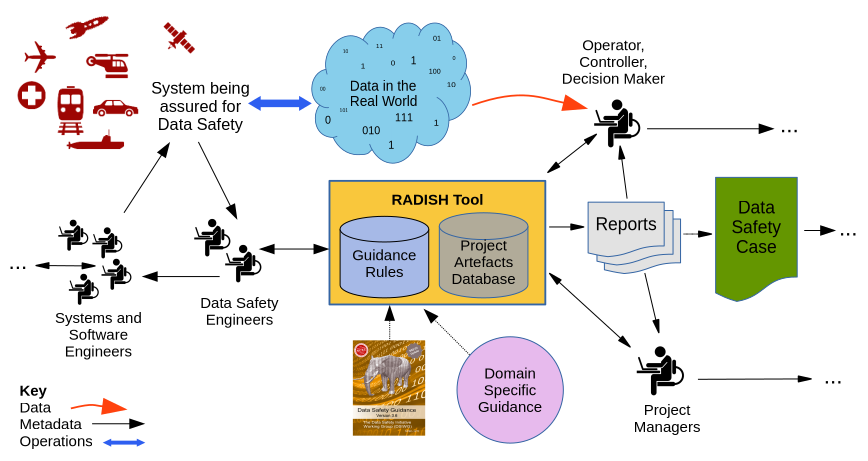
\includegraphics[width=0.85\textwidth]{images/RADISHToolInProjectEnvironment-v02-landscape}
  \caption{Radish within the project environment\index{Radish context}}
  \label{fig:radish}
\end{figure}

\cbend

  %================================================================================
%       Safety Critical Systems Club - Data Safety Initiative Working Group
%================================================================================
%                       DDDD    SSSS  IIIII  W   W   GGGG
%                       D   D  S        I    W   W  G   
%                       D   D   SSS     I    W W W  G  GG
%                       D   D      S    I    WW WW  G   G
%                       DDDD   SSSS   IIIII  W   W   GGG
%================================================================================
%               Data Safety Guidance Document - LaTeX Source File
%================================================================================
%
% Description:
%   Appendix addressing data migration
%================================================================================
\section{Data Migrating, Porting, Importing and Exporting (Informative)}\index{Data Migration}\label{bkm:migration}
%
%\dsiwgSectionQuote{The whole story of migration and what that has done in interconnecting the planet is obviously something I've written about a lot}{Salman Rushdie}
%\dsiwgSectionQuote{Migration is an expression of the human aspiration for dignity, safety and a better future. It is part of the social fabric, part of our very make-up as a human family}{Ban Ki-moon}
%\dsiwgSectionQuote{When it's well managed, migration works in the national interest, for our communities, economy and country.}{Priti Patel}
%\dsiwgSectionQuote{I think migration is a right, but it should be an option, not an obligation}{Nayib Bukele}
\dsiwgSectionQuote{I don't think you'll ever have a perfect world because we humans are prone to error, and so we're always in search of an upgrade}{Henry Rollins}

Migrating, Porting and Import or Export of data between systems is a large and complex topic.
This appendix highlights some of the issues that arise, links to the data safety properties and suggests some mitigations.

\subsection{Introduction and rationale}\label{bkm:migrationintro}
All of these activities involve moving data around, with the expectation that the data will be re-used or re-purposed to some extent after the move. Why is this a problem? Because data can be lost, transformed or misinterpreted due to the migration. If some of this data is safety-related then there is the possibility of creating a data \gls{hazard}. The worst cases are the silent ones: where data is not migrated or modified or changed into something else on migration, and no notification or warning is provided.
In general porting of data, import and export actions can be considered subsets of full data migration activities. 
The following are typical stages of a data migration exercise:
\begin{enumerate}[label=\color{dsiwgAccentColour}\roman*)]
\item Discovery: Identifying what data has to be migrated:
the history, locations, store types, formats and the software currently used to manipulate it.
\item Analysis and Preparation:
Filtering and sorting the data, identifying and cleansing the data, fixing any issues, creating missing data that can’t be moved,
and transforming the data to make it suitable for use in the new system.
\item Trials:
Selected sets or portions of the data are migrated and the results assessed within the new system or context.
This may be extended to include more data through incremental, phased stages.
\item Dry Run:
A full migration is performed to a duplicate system or to the new system in a way that it can be backed out
(ie. the new system can be reverted to its original state), and use of the current system can be continued if necessary.
\item Parallel Running:
Both old and new systems continue running, processing the same data where possible.
This is desirable as it allows quick reversion to the old system in case of failure.
It also allows (sampling) comparison between the old and new systems outputs.
\item Monitoring and Checking:
Operation of the new system is closely monitored and outputs assessed to establish if these would be similar to those produced
by the old system.
\item Move to New:
This is where the old system is switched off and mothballed, and may be subsequently decommissioned and removed.
\end{enumerate}

It is noted that migration is generally between systems
(e.g. a legacy system and a new one) but can be between different instances or environments within the same system,
involving different software, stores or \glspl{database}.

Many moves of data are now to Cloud storage, and the implementation may be largely hidden,
with only software API interfaces available\footnote{It is noted that within a cloud environment mini automated migrations of data are happening all the time as new servers and storage are provisioned by the service provider, software is upgraded, etc. There should be some sort of assurance provided in this case to ensure the data is preserved as required.}.
In this case the options for comparisons may be more limited.
%
\subsection{Migration Cases}
%
There are at least three cases of migration (these simple diagrams are intended to show the end state of the migration, it is acknowledged that there are intermediate stages, as mentioned in \dsiwgRef{Section}{bkm:migrationintro}):
\begin{enumerate}
\item Migration of data from a single old system to a single new system.
This is very common and is the usual upgrade path.
The new system, or indeed both systems, may be in the Cloud.

\begin{figure}[htbp]
  \centering
  
\includegraphics[width=\textwidth/2]{images/migration1.pdf}
  \caption{Simple Migration Path\index{Data Migration!Simple}}
  \label{fig:migration1}
\end{figure}

\item Migration of data from multiple disparate systems to one new system.
This is less common but can be seen in major technology upgrades where it is seen as beneficial to bring together multiple
legacy systems into one new system.

\begin{figure}[htbp]
  \centering
  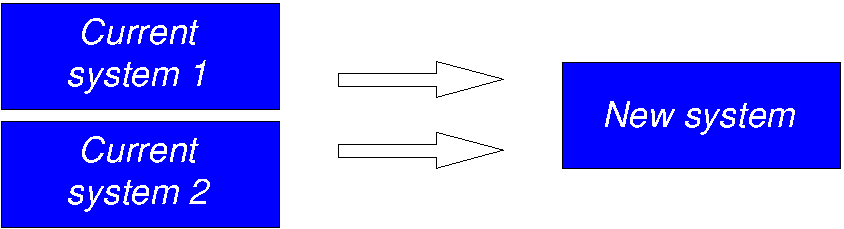
\includegraphics[width=\textwidth/2]{images/migration2.pdf}
  \caption{Many-to-one Migration Path\index{Data Migration!Many to one}}
  \label{fig:migration2}
\end{figure}

\item Migrating data back to an old system in case of failures or to investigate data issues with the new system

\begin{figure}[htbp]
  \centering
  
\includegraphics[width=\textwidth/2]{images/migration3.pdf}
  \caption{Reversion Migration Path\index{Data Migration!Reversion}}
  \label{fig:migration3}
\end{figure}

\end{enumerate}
%
\subsection{Safety Issues due to Migration}
%
The following table summarises some of the safety issues due to migration, maps these to the data safety properties and gives possible mitigations.

\begin{longtable}{|C{\dsiwgColumnWidth{0.10}}|C{\dsiwgColumnWidth{0.24}}|C{\dsiwgColumnWidth{0.20}}|C{\dsiwgColumnWidth{0.20}}|C{\dsiwgColumnWidth{0.20}}|}
  \caption{Safety Issues due to Migration}
  \label{tab:migration}
  \\\hline
  \TableHeadColourCX{No.} & \TableHeadColourCX{Migration Case} & \TableHeadColourCX{What are safety issues in each case?} & \TableHeadColourCX{Mapping to properties/loss of properties} & \TableHeadColourCX{Possible Mitigations (Table \ref{tab:MethodsDataMigration})}\\\hline
  \endfirsthead
  \caption[]{Safety Issues due to Migration (continued)}
  \\\hline
  \TableHeadColourCX{No.} & \TableHeadColourCX{Migration Case} & \TableHeadColourCX{What are safety issues in each case?} & \TableHeadColourCX{Mapping to properties/loss of properties} & \TableHeadColourCX{Possible Mitigations (Table \ref{tab:MethodsDataMigration})}\\\hline
  \endhead
  \multicolumn{5}{r}{\sl Continued on next page}
  \endfoot
  \endlastfoot

1.&
Data format may not map exactly: due to different \gls{database} formats, word lengths, endian issues, etc.&
Data can be lost or discarded, or substituted for defaults. Data may be migrated / imported / exported incorrectly.&
\Gls{integrity}, \gls{completeness}, Format&
DM.02, DM.07, DM.08, DM.09, DM.10\\\hline
%
2.&
Data may not translate exactly: no equivalent data type / record / field type in new system, etc&
Data can be lost or discarded, or substituted for defaults. Data may be migrated / imported / exported incorrectly.&
\Gls{integrity}, \gls{completeness}&
DM.02, DM.04, DM.07, DM.08, DM.09, DM.10\\\hline
%
3.&
Data may not be valid: less numeric range available in new system, etc. Subtype of (2).&
Data can be lost or discarded, or substituted for defaults. Data may be migrated / imported / exported incorrectly.&
\Gls{integrity}, \gls{completeness}&
DM.02, DM.04, DM.07, DM.08, DM.09, DM.10\\\hline
%
4.&
\Gls{metadata} (data about the data) may be lost, including \gls{data dictionary} aspects, derivation, history, signoffs, authorisations,
logs, etc.&
Data may be migrated / imported / exported losing \gls{information}.&
\Gls{traceability}, History&
DM.04, DM.09\\\hline
%
5.&
Data may have a different meaning or interpretation in the new system context.
E.g. if a fluid value is ‘gallons’ and this is migrated from a UK to a US-developed system without applying an adjustment factor.&
Meaning of data can be altered even if migration apparently successful.&
\Gls{consistency}, \gls{fidelity}&
DM.01, DM.04, DM.11\\\hline
%
6.
&
Data may be correctly rejected (detection of error on import / export)&
Data is lost. Not necessarily a problem if notified and fixed.&
\Gls{completeness}&
DM.07, DM.08, DM.09, DM.10\\\hline
%
7.
&
Data may be wrongly filtered or rejected as incompatible&
Correct data is rejected. If data can’t be imported what should happen? a. Rejected and migration halted,
b. Rejected and notified, c. Rejected silently, d. Substituted?&
\Gls{integrity}, \gls{completeness}&
DM.02, DM.03, DM.07, DM.08, DM.09, DM.10\\\hline
%
8.&
Two or more \glspl{item data} may map to the same item in the new system – one may overwrite the other with the last one ‘winning’.&
This is a case of aliasing (See 6.2.2 ref). Data can be lost or discarded. Data may be migrated / imported / exported incorrectly.&
\Gls{integrity}, \gls{completeness}&
DM.02, DM.03, DM.07, DM.08, DM.09, DM.10\\\hline
%
9.&
There may be situations where the data store has to be ‘live’ and the migration / import / export process takes some time.
In this case some data may be out of date and become inconsistent (stale), and \gls{integrity} of the whole \gls{dataset} is lost.&
Data may be migrated / imported / exported incorrectly.&
\Gls{consistency}, \gls{integrity}, \gls{timeliness}&
DM.07, DM.08\\\hline
%
10.&
If a migration is unsuccessful, data changes may have to be undone and stores reverted to original state.
This may not always be possible or completely done.&
Original \gls{dataset} may be corrupted.&
\Gls{consistency}, \Gls{integrity}&
DM.06, DM.07, DM.08\\\hline
%
11.&
The data ‘cleansing’ activity conducted before or during migration may introduce faults.&
The cleansing activity may miss some data faults or may be over-zealous, deleting good values.&
\Gls{integrity}, \gls{completeness}&
DM.07, DM.09, DM.13\\\hline
\end{longtable}

  %================================================================================
%       Safety Critical Systems Club - Data Safety Initiative Working Group
%================================================================================
%                       DDDD    SSSS  IIIII  W   W   GGGG
%                       D   D  S        I    W   W  G   
%                       D   D   SSS     I    W W W  G  GG
%                       D   D      S    I    WW WW  G   G
%                       DDDD   SSSS   IIIII  W   W   GGG
%================================================================================
%               Data Safety Guidance Document - LaTeX Source File
%================================================================================
%
% Description:
%   Section regarding COVID'19, also known as the CCP Virus.
%
%================================================================================
\section{Covid-19\index{Covid-19|textbf} (Informative)} \label{bkm:Covid19}
%\dsiwgSectionQuote{Common sense tells us that the government's attempts to solve large problems more often create new ones. Common sense also tells us that a top-down, one-size-fits-all plan will not improve the workings of a nationwide health-care system that accounts for one-sixth of our economy}{ Sarah Palin}

%\dsiwgSectionQuote{When we make decisions in our personal and professional lives, we typically start with some form of data. The very word ‘data’ derives from the Latin meaning ‘something given’. But who gave it? Where is it from? Should I accept it at face value?}{Adrian Smith CEO of the Alan Turing Institute}

\dsiwgSectionQuote{The public health community wants a safe and effective [COVID-19] vaccine as much as anybody could want it. But the data have to be clear and compelling.}{Michael Osterholm}

\subsection{Covid-19 and Data}
The Covid 19 crisis has highlighted a number of areas where better data and data management could have improved outcomes and hence reduced the death toll. Such pandemic-related data is therefore very much safety-related data. 

Some issues related to Covid-19 data are:
\begin{enumerate}
\item The lack of \index{Consistency!Property Handling}\gls{consistency} and standardisation in handling the data, e.g:
  \begin{enumerate}[label=\color{dsiwgAccentColour}{\alph*.}]
  \item In predictive models\index{Predictive Models} where many assumptions may be wrong, or the algorithms inappropriate
  \item Presentation of statistics in a selective or misleading way
  \item Methods of data collection which may be selective or incomplete. For instance reporting on the number of positive test cases is always misleading, as many people may be asymptomatic with the virus so never get tested.
  \item Calculations and filtering
  \item Allowances for delays in collection or processing
  \item Intentional and unintentional bias
  \item Use of averaging (e.g.\ moving averages) and smoothing of plots hiding sudden increases
  \item Loss of data (e.g.\ in the recent UK Test and Trace system due to old versions of Excel\index{Excel})
  \end{enumerate}
All of which have prevented any meaningful comparisons internationally, even between countries in Western Europe. They also lead to public confusion; this in turn leads to mistrust and a refusal to abide by guidance and regulations. 

\item The poor data within the Test and Trace systems is a major factor in the failure of these systems. If data is not accurate, timely or complete then contacts cannot be traced in time, and the effort put into the activity is wasted. These systems in the UK need huge improvement as there is currently low contact performance and hence very poor outcomes. Background reading on this may be found at this link: \href{https://www.bbc.co.uk/news/health-55008133}{https://www.bbc.co.uk/news/health-55008133}
\end{enumerate}

\subsection{Systems Involved with Covid-19 Data}
Many systems have been created or re-deployed to help manage the pandemic. These systems consume and produce vast amounts of data, some of which is critical and could affect safety of individuals or the general population. Some identified systems are shown in \autoref{tab:PandemicSystems}. For each of these, it is worth thinking through some basic data failure modes, e.g.\ data is lost, late, incorrect or incomplete. For instance if we are running an infection / spread model and we feed it with stale data, then its predictions will clearly be inaccurate.
\begin{longtable}{|L{\dsiwgColumnWidth{0.25}}|L{\dsiwgColumnWidth{0.25}}|L{\dsiwgColumnWidth{0.25}}|L{\dsiwgColumnWidth{0.25}}|}
  \caption{Systems Involving Data Used to Manage the Pandemic}
  \label{tab:PandemicSystems}
  \\\hline
  \endfirsthead
  \caption[]{Systems Involving Data Used to Manage the Pandemic (continued)}
  \\\hline
  \endhead
  \multicolumn{4}{r}{\sl Continued on next page}
  \endfoot\endlastfoot

  Analysis of air flow and particles & 
  Satellite imagery (Wuhan) &
  Video conferencing &
  Risk assessment systems\\\hline
  Infection / spread models (inc new variants) &
  Itinerary systems &
  Remote consultation systems &
  Computational bioinformatics tools\\\hline
  Infra-red / thermal cameras &
  Infection testing systems &
  Ventilators / other patient management devices &
  Appointment systems\\\hline
  Track and Trace apps &
  Antibody testing systems &
  Personal risk profiling apps / systems &
  Border Control / Quarantine systems\\\hline
  Track and Trace back office systems &
  Drug trials systems / data &
  Allocation / reservation / booking systems &
  Risk profiling / prioritising for vaccination\\\hline
  Track and Trace service &
  Ventilation models \& UV sterilisers &
  Models of built environments &
  Digital Twins (systems and biological: lungs, etc.)\\\hline
  Supply chain systems &
  Behavioural models &
  Safety analyses (STAMP/STPA), etc. &
  (Automatic) cleaning systems\\\hline
  Virus aerosols modelling &
  Analysis of delays in system of reporting / actions &
  Modelling / public perception of the disease &
  Virus shedding models\\\hline
%
  Vaccination booking / tracking / monitoring &
  Sanitiser systems &
  Lockdown easing models &
  Vaccination Passports
  \\\hline
%
  Vaccination production data &
  Vaccination trials and reporting data &
  Vaccination ``Yellow Card'' &
  Cross-system data sharing
  \\\hline
%
  PPE testing results &
  Data used to inform public perceptions &
  No coordination across international boundaries --- incompatible systems &
  Use of blockchain to validate Covid and vaccination status\\
  \hline
\end{longtable}

\subsection{Falsification / Misinformation of Data}
One serious and perhaps unexpected aspect of the pandemic is that of misinformation. There are people either in denial of the virus’s dangers, refusing to socially distance or refusing vaccinations. Reasons for these behaviours have generally been driven by intentional misinformation, ignorance, superstition, or economics. Marianna Spring, the BBC’s specialist reporter covering disinformation and social media put the problem of misinformation succinctly when she stated “The problem with misinformation is that it is popular.” See Barack Obama: One election won't stop US `truth decay' --- BBC News at \href{https://www.bbc.co.uk/news/election-us-2020-54910344}{https://www.bbc.co.uk/news/election-us-2020-54910344}. Methods need to be devised or improved to prevent this effect, and to restore trust in carefully managed data. 

\subsection{Rumsfeld’s\index{Rumsfeld, Donald} known unknown\index{Known Unknowns} and unknown unknown\index{Unknown Unknowns} data conundrum}

It is clear that until China reported to the world that Covid 19 had emerged as a threat, that data about the virus was an unknown unknown. However, we know there are thousands of viruses in animals that could pose a threat. These all need analysis and it may be possible to use massive computer analysis of genetic data to identify likely new threats. 
	
A paper was
given by Nick Hales as part of the 2021 Safety-Critical Systems Symposium which gives more detail on this topic {\it“Data Safety in Virus Outbreaks --- Lessons learnt and Recommendations”}~\cite{citation:SCSC161}.

\subsection{Learning}

It is important to learn from these deficiencies because, while Covid 19 has brought tragedies with it, it is unlikely to be the last, or indeed, the most dangerous virus we will face. We must do better next time.

  %================================================================================
%       Safety Critical Systems Club - Data Safety Initiative Working Group
%================================================================================
%                       DDDD    SSSS  IIIII  W   W   GGGG
%                       D   D  S        I    W   W  G   
%                       D   D   SSS     I    W W W  G  GG
%                       D   D      S    I    WW WW  G   G
%                       DDDD   SSSS   IIIII  W   W   GGG
%================================================================================
%               Data Safety Guidance Document - LaTeX Source File
%================================================================================
%
% Description:
%   Proposed alternate ways to customise the assignment of DSALs 
%
%================================================================================
\section{\glsfmtshort{dsal}\index{Assurance Level!Data} Customisation (Informative)} \label{bkm:DsalCustomisation}
%\dsiwgSectionQuote{Common sense tells us that the government's attempts to solve large problems more often create new ones. Common sense also tells us that a top-down, one-size-fits-all plan will not improve the workings of a nationwide health-care system that accounts for one-sixth of our economy}{ Sarah Palin}

\dsiwgSectionQuote{One size does not fit all}{Frank Zappa}

%\dsiwgSectionQuote{When we make decisions in our personal and professional lives, we typically start with some form of data. The very word ‘data’ derives from the Latin meaning ‘something given’. But who gave it? Where is it from? Should I accept it at face value?}{Adrian Smith CEO of the Alan Turing Institute}
\subsection{Introduction}
Within the body of this document, a method has been provided for the assignment of \glspl{dsal}\index{Assurance Level!Data}. However it is anticipated that, as with the methods used for the assignment of safety criteria within system safety analysis, some programmes may find it desirable to develop alternate approaches. This section presents some possible methods for the determination of likelihood. These methods are intended to serve as approaches for consideration when developing project-specific criteria, as these approaches are less generic than that presented through \autoref {tab:Likelihood}, so it is highly likely that customisation will be required.

\subsection{Significance factors}
\label{bkm:SignificanceFactors}
A method of determining likelihood from the different characteristics is to implement a scoring scheme that apportions a quantitative value for each of the characteristics, with the sum giving the total likelihood score. The total score is then compared against a scale, and that in turn determines the overall low, medium or high assessment.

For example, consider the modified version of \autoref {tab:Likelihood} illustrated in \autoref {tab:Likelihood1}

\begin{longtable}{|C{\dsiwgColumnWidth{0.19}}|C{\dsiwgColumnWidth{0.27}}|C{\dsiwgColumnWidth{0.27}}|C{\dsiwgColumnWidth{0.27}}|}
  \caption{Calculation of Likelihood --- Option 1}
  \label{tab:Likelihood1}
  \\\hline
  \TableHeadColour{} & \multicolumn{3}{c|}{\TableHeadColourCX{Score}}\\\cline{2-4}
  \multirow{-2}*{\TableHeadColourCX{}} & \TableHeadColourCX{2} & \TableHeadColourCX{1} & \TableHeadColourCX{0}\\\hline
  \endfirsthead
  \caption[]{Calculation of Likelihood --- Option 1 (continued)}
  \\\hline\TableHeadColour{} & \multicolumn{3}{c|}{\TableHeadColourCX{Score}}\\\cline{2-4}
  \multirow{-2}*{\TableHeadColourCX{}} & \TableHeadColourCX{2} & \TableHeadColourCX{1} & \TableHeadColourCX{0}\\\hline
  \endhead
  \multicolumn{4}{r}{\sl Continued on next page}
  \endfoot
  \endlastfoot
  Proximity & %
    A known use of the data is highly likely to lead to an accident. & %
    A possible use of the data could lead to an accident. & %
    All currently foreseen uses of the data could lead to harm only via lengthy and indirect routes.\\
    \hline
  Dependency & %
    Data is completely relied upon. & %
    Data is indirectly relied upon. & %
    Little reliance on data.\\
    \hline
  Prevention & %
    Difficult or impossible to guard / barrier against errors. & %
    Possible to guard / barrier against errors. & %
    Easy to guard / barrier against error.\\
    \hline
  Detection & %
    Low or no chance of anything else detecting an error. & %
    Some other people / systems are involved in checking the data. & %
    Many other people / systems are involved in checking the data.\\
    \hline
  Correction & %
    Difficult or impossible to correct or workaround errors. & %
    Possible to correct or workaround errors. & %
    Easy to correct or workaround errors.\\
    \hline
\end{longtable}

For each of the characteristics, the applicable assessment of likelihood is then selected and scored. So for example, if it is “Possible to guard / barrier against errors” for Prevention, then the score for that characteristic would be 1. Each characteristic is then scored and they are then summed to give a total score. The range of possible values will run from 0 (all choices in the far right column, favouring low likelihood aspects) through to 10 (all choices in the far left column, favouring high likelihood aspects).

The overall likelihood in the assessed against a scale such that shown in \autoref{tab:Likelihood1a}.

\begin{longtable}{|C{\dsiwgColumnWidth{0.2}}|C{\dsiwgColumnWidth{0.2}}|C{\dsiwgColumnWidth{0.2}}|}
  \caption{Likelihood Assessment}
  \label{tab:Likelihood1a}
  \\\hline
%  \TableHeadColour{} & \multicolumn{3}{c|}{\TableHeadColourCX{Likelihood}}\\\cline{2-4}
  \TableHeadColourCX{Low} & \TableHeadColourCX{Medium} & \TableHeadColourCX{High}\\\hline
  \endfirsthead
  \caption[]{Likelihood Assessment (continued)}
  \\\hline
%  \TableHeadColour{} & \multicolumn{3}{c|}{\TableHeadColourCX{Likelihood}}\\\cline{2-4}
  \TableHeadColourCX{Low} & \TableHeadColourCX{Medium} & \TableHeadColourCX{High}\\\hline
  \endhead
  \multicolumn{3}{r}{\sl Continued on next page}
  \endfoot
  \endlastfoot
  0--2 & 3--6 & >6\\\hline
\end{longtable}


\subsection{Weighted characteristics}
The method presented in
\dsiwgRef{section}{bkm:SignificanceFactors}
may be enhanced to provide a more holistic overall assessment of the likelihood based on all characteristics. Note that the scheme in
\dsiwgRef{section}{bkm:SignificanceFactors}
allocated equal significance to each of the characteristics. This method could be further refined if necessary to apply weightings to each of the characteristics, as shown in \autoref{tab:Likelihood2}.

\begin{longtable}{|C{\dsiwgColumnWidth{0.19}}|C{\dsiwgColumnWidth{0.15}}|C{\dsiwgColumnWidth{0.20}}|C{\dsiwgColumnWidth{0.20}}|C{\dsiwgColumnWidth{0.20}}|}
  \caption{Calculation of Likelihood --- Option 2}
  \label{tab:Likelihood2}
  \\\hline
  \TableHeadColour{} & \TableHeadColour{} & \multicolumn{3}{c|}{\TableHeadColourCX{Score}}\\\cline{2-4}
  \multirow{-2}*{\TableHeadColourCX{}} & \TableHeadColourCX{Weighting} & \TableHeadColourCX{2} & \TableHeadColourCX{1} & \TableHeadColourCX{0}\\\hline
  \endfirsthead
  \caption[]{Calculation of Likelihood --- Option 2 (continued)}
  \\\hline
  \TableHeadColour{} & \TableHeadColour{} & \multicolumn{3}{c|}{\TableHeadColourCX{Score}}\\\cline{2-4}
  \multirow{-2}*{\TableHeadColourCX{}} & \TableHeadColourCX{Weighting} & \TableHeadColourCX{2} & \TableHeadColourCX{1} & \TableHeadColourCX{0}\\\hline
  \endhead
  \multicolumn{4}{r}{\sl Continued on next page}
  \endfoot
  \endlastfoot
  Proximity & %
    1.5 & %
    \bf A known use of the data is highly likely to lead to an accident. & %
    A possible use of the data could lead to an accident. & %
    All currently foreseen uses of the data could lead to harm only via lengthy and indirect routes.\\
    \hline
  Dependency & %
    1.0 & %
    Data is completely relied upon. & %
    \bf Data is indirectly relied upon. & %
    Little reliance on data.\\
    \hline
  Prevention & %
    1.3 & %
    \bf Difficult or impossible to guard / barrier against errors. & %
    Possible to guard / barrier against errors. & %
    Easy to guard / barrier against error.\\
    \hline
  Detection & %
    0.7 & %
    Low or no chance of anything else detecting an error. & %
    Some other people / systems are involved in checking the data. & %
    \bf Many other people / systems are involved in checking the data.\\
    \hline
  Correction & %
    0.5 & %
    Difficult or impossible to correct or workaround errors. & %
    Possible to correct or workaround errors. & %
    \bf Easy to correct or workaround errors.\\
    \hline
\end{longtable}

The total score is then calculated by first multiplying the individual characteristic’s score by the weighting before summing all the values. For example, if the selections highlighted in bold were made, then the score would be
$$(1.5 \times 2) + (1.0 \times 1) + (1.3 \times 2) + (0.7 \times 0) + (0.5 \times 0) = 6.6$$
resulting in a {\sl High} assessment rather than the {\sl Medium} that would result with no weighting. This is because Proximity and Prevention are considered (in this particular example) more important than Detection and Correction. The weightings within a project-specific version of this table would be chosen by the organization to suit the particular scenario under consideration.

        \settocdepth{subsection}
  %================================================================================
%       Safety Critical Systems Club - Data Safety Initiative Working Group
%================================================================================
%                       DDDD    SSSS  IIIII  W   W   GGGG
%                       D   D  S        I    W   W  G   
%                       D   D   SSS     I    W W W  G  GG
%                       D   D      S    I    WW WW  G   G
%                       DDDD   SSSS   IIIII  W   W   GGG
%================================================================================
%               Data Safety Guidance Document - LaTeX Source File
%================================================================================
%
% Description:
%   Acronyms, Definitions and Glossary section.
%
%================================================================================
\section{Acronyms, Definitions and Glossary (Discursive)} \label{bkm:acronyms}

\dsiwgSectionQuote{The plural of anecdote is not data.}{Mark Berkoff}

%
%Uncomment the following to have LaTeX automatically list the acronyms and
%glossary entries used in this document, as indicated by the \gls, \glspl,
%\acrshort, and \acrfull commands. (All defined in the file 'glossary.tex'
% Note: some of these now done, where the Perfectit tool identified issues
% in the existing document. I think it should be \acrlong, not \acrfull.
% New command \acrentry{} introduced to reduce repetition
%
%THIS WILL BE LEFT UNTIL THE NEXT VERSION (2.X OR 3.0)
%
%\printglossary[type=acronym]
%\printglossary

\subsection{Acronyms}
\begin{longtable}{|L{\dsiwgColumnWidth{0.2}}|L{\dsiwgColumnWidth{0.8}}|}
  \hline\TableHeadColour{Acronym} & \TableHeadColour{Expansion}\\\hline
  \endfirsthead
  \hline\TableHeadColour{Acronym} & \TableHeadColour{Expansion}\\\hline
  \endhead
  \endfoot\endlastfoot

  AAL & Above Aerodrome Level\\\hline
  \acrentry{adiru}
  \acrentry{aoa}
  ARP & Aerospace Recommended Practice\\\hline
  ARQ & Automatic Repeat-reQuest\\\hline
  ATM & Air Traffic Management\\\hline
  ATSB & Australian Transport Safety Bureau\\\hline
  BIT(E) & Built-In Test (Equipment)\\\hline
	CFIT & Controlled Flight Into Terrain\\\hline
  CNS & Communications, Navigation, Surveillance\\\hline
  CoD & Certificate of Design\\\hline
  \acrentry{cots}
  \acrentry{cpu}
  CRC & Cyclic Redundancy Check\\\hline
  CSV & Comma Separated Variable\\\hline
  CT & Computed Tomography\\\hline
  DCB & Data Coordination Board\\\hline
  DME & Distance Measuring Equipment\\\hline
	DOC & Department Of Corrections\\\hline
  DRACAS & Defect Reporting And Corrective Action System\\\hline
  \acrentry{dsal}
  DSG & Data Safety Guidance\\\hline
  \acrentry{dsiwg}
  \acrentry{dsmp}
  ECS & Electronic Chart System\\\hline
  ECU & Electronic Control Unit\\\hline
	EDM & Entry Demonstrator Module\\\hline
	EGPWS & Enhanced Ground Proximity Warning System\\\hline
  EHR & Electronic Health Record\\\hline
  ENC & Electronic Navigational Chart\\\hline
  ESA & European Space Agency\\\hline
	FAA & Federal Aviation Administration\\\hline
  \acrentry{fcpc}
  \acrentry{fdal}
  FMGS & Flight Management Guidance System\\\hline
  FMS & Flight Management System\\\hline
	GCS & Ground Control Station\\\hline
  GP & General Practitioner\\\hline
	GPS & Global Positioning System\\\hline
  GTOLS & GPS Take-off and Landing System\\\hline
  \acrentry{hazop}
	HSE & Health and Safety Executive\\\hline
  HUMS & Health and Usage Monitoring System\\\hline
	ICD & Interface Control Document\\\hline
  \acrentry{icao}
  IDAL & Item \index{Assurance Level!Development}Development Assurance Level\\\hline
  IMC & Instrument Meteorological Conditions\\\hline
	IMU & Inertial Measurement Unit\\\hline
  \acrentry{ip}
	IRS & Inertial Reference System\\\hline
  ISO & International Organization for Standardization\\\hline %note official name is with z's
	IV & Intravenous\\\hline
  LHR & London Heathrow\\\hline
	MAIB & Maritime Accident Investigation Board (\textit{or} Branch)\\\hline
        \acrentry{mca}
        ML & Machine Learning\\\hline
	MSAW & Minimum Safe Altitude Warning\\\hline
  NaN & Not a Number\\\hline
  NOTAM & Notice to Airmen\\\hline
  \acrentry{odr}
  OOW & Officer Of the Watch\\\hline
  OSI & Open Systems Interconnection\\\hline
  \acrentry{pcr}
	RDA & Radar Doppler Altimeter\\\hline
	SAR & Search And Rescue\\\hline
  \acrentry{saswg}
  \acrentry{scsc}
  SIL & Safety Integrity Level\\\hline
  SMP & Safety Management Plan\\\hline
  SOP & Standard Operating Procedure\\\hline
  \acrentry{sotif}
  \acrentry{sss}
	TCAS & Traffic Collision Avoidance System\\\hline
	UAS & Unmanned Air System\\\hline
	USB & Universal Serial Bus\\\hline
  \acrentry{vhf}
  \acrentry{vmc}
  VMS & Voyage Management System\\\hline
  VOR & VHF Omnidirectional Range\\\hline
  XML & eXtensible Markup Language\\\hline
\end{longtable}

\clearpage %Manual page break
\subsection{Definitions \& Glossary}
% Odd values required in multirow, to adjust text to centre of multi-line definitions
\begin{longtable}{|p{\dsiwgColumnWidth{0.2}}|L{\dsiwgColumnWidth{0.6}}|L{\dsiwgColumnWidth{0.2}}|}
  \hline\TableHeadColour{} & \TableHeadColour{Definition} & \TableHeadColour{Source}\\\hline
  \endfirsthead
  \hline\TableHeadColour{} & \TableHeadColour{Definition} & \TableHeadColour{Source}\\\hline
  \endhead
  \endfoot\endlastfoot
  \multicolumn{3}{|l|}{\TableDimColour{A}}\\%{\cellcolor{dsiwgAccentColour} \color{white} A}\\
  \hline
  {} & Closeness of agreement between a test result and the accepted reference value. Note that a test result can be observations or measurements. & ISO 19113:2005 \cite{citation:ISO19113}\\
  \cline{2-3}
  \multirow{-3.5}*{\index{Accuracy Property|textbf}Accuracy} & A degree of conformance between the estimated or measured value and the true value. & (EU) No 73/2010 \cite{citation:EU732010}\\
  \hline
  \index{Artefact, Data|textbf} (data) Artefact & An item, or collection of items, that provides a useful perspective on data
  generated, processed or consumed by a system. & \\
  \hline
  \index{Accuracy, Temporal\textbf}Accuracy (temporal) & Correctness of the temporal references of an item (reporting of error in time measurement). Correctness of ordered events or sequences, if reported. Validity of data with respect to time. & ISO 19138:2006 \cite{citation:ISO19138}\\
  \hline
  {} & The required \index{Assurance Level}assurance level for the aeronautical data process is identified, based on the overall system architecture through allocation of risk determined using a preliminary \index{Safety Assessment!System}system safety assessment. & RTCA/DO-200A \cite{citation:ED76}\\
  \cline{2-3}
  \multirow{-4.5}*{\index{Assurance Level!Data|textbf}(data) Assurance Level} & An indication of how much assurance is required (commensurate to risk) before deploying software into an operational system. & J Spriggs, based on (EC) No 482/2008 \cite{citation:EC4822008}\\
  \hline
  Adaptation Data\index{Adaptation Data} & Data used to customise elements of the Air Traffic Management System for their designated purpose.
  Adaptation data\index{Adaptation Data} is used to customise elements of the CNS / ATM system for its designated purpose at a specific location.
  These systems are often configured to accommodate site-specific characteristics.
  These site dependencies are developed into sets of adaptation data\index{Adaptation Data}.
  Adaptation data\index{Adaptation Data} includes data that configures the software for a given geographical site, and data that configures a workstation to the preferences and / or functions of an operator.
  Examples include, but are not limited to:
  \begin{enumerate}
  \item Geographical Data - latitude and longitude of a radar site.
  \item Environmental Data - operator selectable data to provide their specific preferences.
  \item Airspace Data - sector-specific data.
  \item Procedures - operational customisation to provide the desired operational role.
  \end{enumerate}
  Adaptation data\index{Adaptation Data} may take the form of changes to either database parameters or take the form of pre-programmed options.
  In some cases, adaptation data\index{Adaptation Data} involves re-linking the code to include different libraries.
  Note that this should not be confused with recompilation in which a completely new version of the code is generated. & ED-153 \cite{citation:ED153}\\
  \hline
  & A representation of aeronautical facts, concepts or instructions in a formalized manner suitable for communication, interpretation or processing. & (EU) No 73/2010 \cite{citation:EU732010}\\
  \cline{2-3}
  \multirow{-3.5}*{Aeronautical Data} & Data used for aeronautical applications such as navigation, flight planning, flight simulators, terrain awareness, and other purposes. & RTCA/DO-178C \cite{citation:ED12C}\\
  \hline
  Availability\index{Availability Property|textbf} & The property of being accessible and usable upon demand by an authorized entity. & ISO27001:2013 \cite{citation:ISO27001:2013}\\
  \hline
  \multicolumn{3}{|l|}{\TableDimColour{B}}\\
  \hline
  \multicolumn{3}{|l|}{\TableDimColour{C}}\\
  Completeness\index{Completeness!Property|textbf} & Completeness of the data provided. & RTCA/DO-200A \cite{citation:ED76}\\
  \hline
  & Data that configures a generic software system to a particular instance of its use. & (EC) No 482/2008 \cite{citation:EC4822008}\\
  \cline{2-3}
  \multirow{-2.5}*{Configuration Data} & Data that configures a generic software system to a particular instance of its use (e.g., data for flight data processing system for a particular airspace, by setting the positions of airways, reporting points, navigation aids, airports and other elements important to air navigation). & ED-153 \cite{citation:ED153}\\
  \hline
  Confidentiality & The property that information is not made available or disclosed to unauthorized individuals, entities, or processes. & ISO27001:2013 \cite{citation:ISO27001:2013}\\
  \hline
  (data) Consistency\index{Consistency!Property|textbf} & The property that the data adheres to a common world view (e.g., units). &  \\

  \hline
  (data) Continuity\index{Continuity Property|textbf} & The property that the data is continuous and regular without gaps or breaks. &  \\

  \hline
  (data) Correctness & Completeness, \index{Consistency!Self}self-consistency, protection against alteration or corruption and \index{Consistency!With Requirements}consistency with the functional requirements of the data-driven system. & IEC 61508 Part 3 \cite{citation:iec615083}\\
  \hline
  (data) Coupling & The dependence of a software component on data not exclusively under the control of that software component. & RTCA/DO-178C \cite{citation:ED12C}\\ 
  \hline
  (data) Criticality & Classification of data by the potential effect of erroneous data on the expected operation that is supported by that data. & RTCA/DO-200A \cite{citation:ED76}\\ 
  \hline
  Critical Data & Data with an \index{Integrity Property}integrity level as defined in Chapter 3, Section 3.2 point 3.2.8(a) of Annex 15 to the Chicago Convention, i.e., \index{Integrity Property}integrity level one in one hundred million: there is a high probability when using corrupted critical data that the continued safe flight and landing of an aircraft would be severely at risk with the potential for catastrophe. & (EU) No 73/2010 \cite{citation:EU732010}\\ 
  \hline
  Customisation (data) & Data used to configure a system or component. & Def(Aust)5679 \cite{citation:DEFOz}\\ 
  \hline
  \multicolumn{3}{|l|}{\TableDimColour{D}}\\
  \hline
  & A thing given or granted; something known or assumed as fact, and made the basis of reasoning or calculation; an assumption or premiss from which inferences are drawn. & Oxford English Dictionary (OED)\\
  \cline{2-3}
  \multirow{-3.5}*{Data} & A reinterpretable representation of information in a formalized manner suitable for communication, interpretation or processing. & ISO/IEC 2382 \cite{citation:ISO23821}\\
  \hline
  Database & A set of data, part or the whole of another set of data, consisting of at least one file that is sufficient for a given purpose or for a given data processing system. & RTCA/DO-178C \cite{citation:ED12C}\\
  \hline
  & An `Aeronautical Data Chain' is a conceptual representation of the path that a set, or element of aeronautical data takes from its creation to its end use. An aeronautical data chain is a series of interrelated links wherein each link provides a function that facilitates the origination, transmission and use of aeronautical data for a specific purpose. & RTCA/DO-200A \cite{citation:ED76}\\
  \cline{2-3}
  & A collection of organizational data processing functions, where data is transferred from one chain participant to another between data origination and end use. & P. Ensor \cite{citation:Ensor2009}\\
  \cline{2-3}
  \multirow{-8}*{Data Chain} & Any combination of two or more data elements, data items, data codes, and data abbreviations in a prescribed sequence to yield meaningful information; for example, ``date'' consists of data elements year, month, and day. & McGraw-Hill Dictionary \cite{citation:McGrawHill}\\
  \hline
  (data) Dictionary & The detailed description of data, parameters, variables, and constants used by the system. & RTCA/DO-178C \cite{citation:ED12C}\\
  \hline
  Data-Driven Systems & System which relies upon configuration data or lookup tables to define the functionality of the system. & IEC 61508 Part 4 \cite{citation:iec615084}\\
  \hline
  Data-intensive System & Systems which make extensive use of large amounts of data. & N. Storey \cite{citation:StoreyFaulkner20031}\\
  \hline
  \multicolumn{3}{|l|}{\TableDimColour{E}}\\
  \hline
  & Discrepancy with the universe of discourse. & ISO 19138:2006 \cite{citation:ISO19138}\\
  \cline{2-3}
  \multirow{-2}*{(data) Error} & Discrepancy between a data value and the true, specified or theoretically correct value or condition. & P. Ensor \cite{citation:Ensor2009}\\
  \hline
  Essential Data & Data with an \index{Integrity Property}integrity level as defined in Chapter 3, Section 3.2 point 3.2.8(b) of Annex 15 to the Chicago Convention, i.e., \index{Integrity Property}integrity level one in one hundred thousand: there is a low probability when using corrupted essential data that the continued safe flight and landing of an aircraft would be severely at risk with the potential for catastrophe. & (EU) No 73/2010 \cite{citation:EU732010}\\
  \hline
  \multicolumn{3}{|l|}{\TableDimColour{F}}\\
  \hline
  \raggedright{(data) Fidelity/ Representation\index{Fidelity/Representation Property|textbf}} & The property describing how well the data maps to the real world entity it is trying to model. &  \\
  \hline

  \multicolumn{3}{|l|}{\TableDimColour{G}}\\
  \hline
  \multicolumn{3}{|l|}{\TableDimColour{H}}\\
  \hline
  (data) Hazard & Use of data in the context of a system that could lead to an accident. & SCSC Data Safety Initiative Working Group\\
  \hline
  %  Hazard Log & A hazard log is a record keeping tool applied to tracking all hazard analysis, risk assessment and risk reduction activities for the whole-of-life of a safety-related system.&\\
  Hazard Log & A Hazard Log records all hazard analysis,
  safety risk assessment and safety risk reduction activities for the ``whole-of-life'' of a safety-related system. &\\
  \hline
  \multicolumn{3}{|l|}{\TableDimColour{I}}\\
  \hline
  & Knowledge communicated concerning some particular fact, subject, or event; that of which one is apprised or told - intelligence, news - as contrasted with data. & Oxford English Dictionary (OED)\\
  \cline{2-3}
  \multirow{-3.5}*{Information} & Knowledge that has a contextual meaning. & ISO/IEC 2382  \cite{citation:ISO23821}\\
  \hline
  Information (aeronautical) & Information resulting from the assembly, analysis and formatting of aeronautical data. & (EU) No 73/2010 \cite{citation:EU732010}\\
  \hline
  & The assurance that a data element retrieved from a storage system has not been corrupted or altered in any ways since the original data entry\index{Data!Entry} or latest authorised amendment. & RTCA/DO-200A \cite{citation:ED76}\\
  \cline{2-3}
  & The degree of assurance that a data item and its value have not been lost or altered since the data origination or authorised amendment. & (EU) No 73/2010 \cite{citation:EU732010}\\
  \cline{2-3}
  & The degree of undetected (at system level) non-conformity of the input value of the data item with its output value. & (EU) No 1207/2011 \cite{citation:EU12072011}\\
  \cline{2-3}
  \multirow{-7}*{\index{Integrity Property|textbf}(data) Integrity} & The property of protecting the \index{Accuracy Property}accuracy and completeness of assets, i.e., that which has value to the organization. & ISO27001:2013 \cite{citation:ISO27001:2013}\\
  \hline
  (data) Item & Single attribute of a complete data set, which is allocated a value that defines its current status. & (EU) No 73/2010 \cite{citation:EU732010}\\
  \hline
  \multicolumn{3}{|l|}{\TableDimColour{J}}\\
  \hline
  \multicolumn{3}{|l|}{\TableDimColour{K}}\\
  \hline
  \multicolumn{3}{|l|}{\TableDimColour{L}}\\
  \hline
  \multicolumn{3}{|l|}{\TableDimColour{M}}\\
  \hline
  Metadata & Data that represents information about data itself. Note that one should distinguish between ``Structural Metadata'', which is data about the design and specification of data structures (and is more properly called ``data about the containers of data'') and ``Descriptive Metadata'', which is about individual instances of application data, the data content. & J. Inge \cite{citation:inge2008improving}\\
  \hline
  \multicolumn{3}{|l|}{\TableDimColour{N}}\\
  \hline
  \multicolumn{3}{|l|}{\TableDimColour{O}}\\
  \hline
  (data) Origination & Creation of a new data item with its associated value, the modification of the value of an existing data item or the deletion of an existing data item. & (EU) No 73/2010 \cite{citation:EU732010}\\
  \hline
  (data) Owner\index{Data!Owner}\index{Owner, Data|see{Data, Owner}} & The individual or organization responsible for a particular Data Artefact, or collection of Data Artefacts. & \\
  \hline
  \multicolumn{3}{|l|}{\TableDimColour{P}}\\
  \hline
  (data) Product & Dataset or dataset series that conforms to a data product specification. & BS EN ISO 19131:2008 \cite{citation:ISO19131}\\
  \hline
  \multicolumn{3}{|l|}{\TableDimColour{Q}}\\
  \hline
  & A degree or level of confidence that the data provided meet the requirements of the user. These requirements include levels of accuracy\index{Accuracy Property}, resolution\index{Resolution Property}, assurance level\index{Assurance Level}, traceability, timeliness\index{Timeliness Property}, completeness, and format. & RTCA/DO-200A \cite{citation:ED76}\\
  \cline{2-3}
  & Process by which the Electronic Chart Systems (ECS) Database is produced, the source materials, the resolution\index{Resolution Property} and reproduction \index{Accuracy Property}accuracy of chart features, and the correctness and completeness of data. & ISO 19379:2003 \cite{citation:ISO19379}\\
  \cline{2-3}
  \multirow{-8}*{(data) Quality} & A degree or level of confidence that the data provided meets the requirements of the data user in terms of \index{Accuracy Property}accuracy, resolution\index{Resolution Property} and \index{Integrity Property}integrity. & (EU) No 73/2010 \cite{citation:EU732010}\\
  \hline
  (data) Property\index{Property!Data} & A characteristic that can be exhibited by a Data Artefact. & \\
  \hline
  \raggedright{(data) Quality Attributes} & Accuracy\index{Accuracy Property}, resolution\index{Resolution Property}, \index{Assurance Level}assurance level, traceability, timeliness\index{Timeliness Property}, completeness and format. & RTCA/DO-200A \cite{citation:ED76}\\
  \hline
  \multicolumn{3}{|l|}{\TableDimColour{R}}\\
  \hline
  & The smallest difference between two adjacent values that can be represented in a data storage, display or transfer system. & RTCA/DO-200A \cite{citation:ED76}\\
  \cline{2-3}
  \multirow{-2.5}*{Resolution}\index{Resolution Property} & A number of units or digits to which a measured or calculated value is expressed and used. & (EU) No 73/2010 \cite{citation:EU732010}\\
  \hline
  Response\index{Response} & The way in which an identified risk is addressed; possible responses include avoid/eliminate, treat, or accept as sufficiently low. & \\
  \hline
  Routine Data & Data with an \index{Integrity Property}integrity level as defined in Chapter 3, Section 3.2 point 3.2.8(b) of Annex 15 to the Chicago Convention, i.e., \index{Integrity Property}integrity level one in one thousand: there is a very low probability when using corrupted routine data that the continued safe flight and landing of an aircraft would be severely at risk with the potential for catastrophe. & (EU) No 73/2010 \cite{citation:EU732010}\\
  \hline
  \multicolumn{3}{|l|}{\TableDimColour{S}}\\
  \hline
  \raggedright{(data) Safety Assessment}\index{Safety Assessment!Data} & The process of explicitly considering data as part of a system safety assessment, via the means of Data Artefacts, Data Properties and Data Safety Assurance Levels. & \\
  \hline
  \raggedright{(data) Safety Assurance Level}\index{Assurance Level!Data} & An indication of the level of rigour with which relevant Data Properties should be demonstrated for appropriate Data Artefacts. & \\
  \hline
  \raggedright{(data) Safety Requirement}\index{Safety Requirement!Data} & A requirement to implement an approach specifically designed to achieve, maintain or demonstrate a Data Property (or Properties) for a given Data Artefact (or Artefacts). & \\
  \hline
  Sequencing\index{Sequencing, Data|textbf} & The property that the data is preserved in the order required. &\\
  \hline
  (data) Set & Identifiable collection of data. Note that a dataset may be a smaller grouping of data which, though limited by some constraint such as spatial extent or feature type, is located physically within a larger dataset. Theoretically, a dataset may be as small as a single feature or feature attribute contained within a larger dataset. A hardcopy map or chart may be considered a dataset. & BS EN ISO 19131:2008 \cite{citation:ISO19131}\\
  \hline
  \raggedright{Software Lifecycle Data} & Data that is produced during the software lifecycle\index{Lifecycle!Software} to plan, direct, explain, define, record, or provide evidence of activities (including the software product itself). This data enables the software lifecycle\index{Lifecycle!Software} processes, system or equipment approval and post-approval modification of the software product. & ED-153 \cite{citation:ED153}\\
  \hline
  Stakeholder\index{Stakeholder|textbf} & An individual or organization that has some relationship to the system, possibly including a power of veto. & \\
  \hline
  \multicolumn{3}{|l|}{\TableDimColour{T}}\\
  \hline
  & A measure of the time delay between a change in the real world and the associated database update being available to the user. & P. Ensor \cite{citation:Ensor2009}\\ 
  \cline{2-3}
  \multirow{-2.5}*{Timeliness}\index{Timeliness Property} & The difference between the time of output of a data item and the time of applicability of that data item. & (EU) No 1207/2011 \cite{citation:EU12072011}\\ 
  \hline
  Traceability & Ability to determine the origin of the data. & RTCA/DO-200A \cite{citation:ED76}\\ 
  \hline
  Trace (data) & Data providing evidence of traceability of development and verification processes software lifecycle\index{Lifecycle!Software} data without implying the production of any particular artefact. Trace data may show linkages, for example, through the use of naming conventions or through the use of references or pointers either embedded in or external to the software lifecycle\index{Lifecycle!Software} data. & RTCA/DO-178C \cite{citation:ED12C}\\ 
  \hline
  Treatment\index{Treatment!Risk|textbf} & An action taken to reduce or control risk. & \\
  \hline
  \multicolumn{3}{|l|}{\TableDimColour{U}}\\
  \hline
  \multicolumn{3}{|l|}{\TableDimColour{V}}\\
  & The activity whereby a data element is checked as having a value that is fully applicable to the identity given to the data element, or a set of data elements that is checked as being acceptable for their purpose. & RTCA/DO-200A \cite{citation:ED76}\\
  \cline{2-3}
  \multirow{-3.5}*{(data) Validation} & Process of ensuring that data meets the requirements for the specified application or intended use. & (EU) No 73/2010 \cite{citation:EU732010}\\
  \hline
  Validity (period of) & Period between the date and time on which aeronautical information is published and the date and time on which the information ceases to be effective. & (EU) No 73/2010 \cite{citation:EU732010}\\
  \hline
  (data) Verification & Evaluation of the output of an aeronautical data process to ensure correctness and \index{Consistency!With Inputs}consistency with respect to the inputs and applicable data standards, rules and conventions used in that process. & (EU) No 73/2010 \cite{citation:EU732010}\\
  \hline
  Verifiability\index{Verifiability Property|textbf} & The property of the data that it can be checked and its properties demonstrated to be correct &\\
  \hline
  \multicolumn{3}{|l|}{\TableDimColour{W}}\\
  \hline
  \multicolumn{3}{|l|}{\TableDimColour{X}}\\
  \hline
  \multicolumn{3}{|l|}{\TableDimColour{Y}}\\
  \hline
  \multicolumn{3}{|l|}{\TableDimColour{Z}}\\
  \hline
\end{longtable}

  %================================================================================
%       Safety Critical Systems Club - Data Safety Initiative Working Group
%================================================================================
%                       DDDD    SSSS  IIIII  W   W   GGGG
%                       D   D  S        I    W   W  G   
%                       D   D   SSS     I    W W W  G  GG
%                       D   D      S    I    WW WW  G   G
%                       DDDD   SSSS   IIIII  W   W   GGG
%================================================================================
%               Data Safety Guidance Document - LaTeX Source File
%================================================================================
%
% Description:
%   References section.
%
%================================================================================

\section{References (Discursive)} \label{bkm:references}


\dsiwgSectionQuote{Data opportunities multiply as the data is transformed.}{Sun Tzu misquoted}
%
%Simply let LaTeX and BiBTeX do all of the work...
%
% Original format. Doesn't support ISBN.
%\bibliographystyle{ieeetr}
% is-unsrt is part of Nelson Beebe's set of extensions to include ISBN
\bibliographystyle{is-unsrt}
\bibliography{main}

  %================================================================================
%       Safety Critical Systems Club - Data Safety Initiative Working Group
%================================================================================
%                       DDDD    SSSS  IIIII  W   W   GGGG
%                       D   D  S        I    W   W  G   
%                       D   D   SSS     I    W W W  G  GG
%                       D   D      S    I    WW WW  G   G
%                       DDDD   SSSS   IIIII  W   W   GGG
%================================================================================
%               Data Safety Guidance Document - LaTeX Source File
%================================================================================
%
% Description:
%   DSIWG History section.
%
%================================================================================
\section{DSIWG History (Discursive)} \label{bkm:history}

\dsiwgSectionQuote{If we have data, let's look at data. If all we have are opinions, let's go with mine.}{Jim Barksdale}

The task of developing generally applicable, pan-sector guidance for data safety issues was taken on by the Data Safety Initiative Working Group (\gls{dsiwg}) of the \glsfirst{scsc}. The \gls{dsiwg}'s work started with a seminar \textit{``How to Stop Data Causing Harm''}, which was held in December 2012; material from this seminar is available at: (\href{http://scsc.org.uk/e209}{http://scsc.org.uk/e209}) (accessed 30 October 2017). The first meeting of the group agreed the following vision: 

\begin{quote}
  \dsiwgTextBF{\dsiwgTextIT{To have clear guidance on how data (as distinct from software and hardware) should be managed in a safety-related context, which will reflect emerging best practice.}}
\end{quote}

The group, comprising industry, academics, government and independent consultants,
produced an initial guidance document in January 2014.
A subsequent version of the document was released in January 2015,
with a second seminar \dsiwgTextIT{''How to Stop Data Causing Harm: What You Need to Know''} held in December 2015;
material from this seminar is available at: \href{http://scsc.org.uk/e343}{http://scsc.org.uk/e343} (accessed 17 January 2023).
Details pertaining to a third data safety seminar \dsiwgTextIT{``Data Safety Evolution''} that was held in November 2019 may be found at
\href{https://scsc.uk/e651}{https://scsc.uk/e651}
(accessed 17 January 2023).
To help disseminate information, members of the \gls{dsiwg} have presented papers relating to data safety in a number of fora,
including the Safety-critical Systems Symposium (SSS).

Further revisions of the guidance document, which include new material generated during and as a consequence of \gls{dsiwg} meetings, were issued in January 2016, January 2017 and in January 2018.

The January 2018 release was version 3.0 and the \gls{dsiwg} decided to keep this version ``current'' for several years, to enable users to demonstrate compliance against a fixed target. However it was also necessary to keep the document up to date and address user feedback, particularly where this could improve the usability of the document. The next two versions were therefore kept in alignment with version 3.0, with all section numbers in the body of the document remaining constant.

This latest update is version 3.6, the sixth update of the January 2018 version 3.0, and was released in February 2024.

  %================================================================================
%       Safety Critical Systems Club - Data Safety Initiative Working Group
%================================================================================
%                       DDDD    SSSS  IIIII  W   W   GGGG
%                       D   D  S        I    W   W  G   
%                       D   D   SSS     I    W W W  G  GG
%                       D   D      S    I    WW WW  G   G
%                       DDDD   SSSS   IIIII  W   W   GGG
%================================================================================
%               Data Safety Guidance Document - LaTeX Source File
%================================================================================
%
% Description:
%   Contributors section.
%
%================================================================================
\section{Contributors (Discursive)} \label{bkm:contributors}

\dsiwgSectionQuote{Without data, you're just another person with an opinion.}{W. Edwards Deming}

This document has had the benefit of contributions from a large number of people, who work for a variety of organisations, which collectively span a range of different sectors. Note that contributions  have been made on an individual basis and, in particular, the inclusion of an organisation in the following list does \dsiwgTextBF{not} necessarily mean that organisation agrees with the entire contents of the document.

Updates to the most recent version of the document were written by:
\begin{itemize}
  \item Nick Hales
  \item Paul Hampton, CGI IT UK Ltd
  \item Mike Parsons, Ebeni and SCSC
  \item Tim Rowe, TGR Safety Management Ltd
  \item Alan Simpson, Ebeni
  \item Mark Templeton, Arcade Experts Ltd
\end{itemize}

%Review comments were gratefully received from the following:
%\begin{itemize}
%\item Oscar Slotosch, Validas AG
%\item Andy Williams
%\end{itemize}
  
%\clearpage %Manual page break
In addition to the above,
contributors to earlier versions upon which this document is based include the following
(the organisations listed were correct at the time of their contribution)
:
\begin{itemize}
  \item Mike Ainsworth, Ricardo
  \item Rob Ashmore, Dstl
  \item Michael Aspaturian, EDF Energy
  \item Divya Atkins, Mission Critical Applications
  \item Martin Atkins, Mission Critical Applications
  \item Janette Baldwin, Thales UK
  \item Dave Banham, Blackberry QNX
  \item Ian Bingham
  \item John Bragg, MBDA UK Ltd
  \item Jennifer Brain, Wood plc
  \item Eric Bridgstock
  \item Simon Brown, QinetiQ
  \item Dermot Martin Burke, BAE Systems
  \item Dale Callicott, DKCSC Ltd
  \item John Carter, General Dynamics
  \item Martyn Clarke, SCSS Ltd
  \item Steve Clugston, TSC
  \item Robin Cook, Thales
  \item Davin Crowley-Sweet, Highways England
  \item Dijesh Das, AMEC / BAE Systems
  \item Duncan Dowling, DARD
  \item Andrew Eaton
  \item Ashraf El-Shanawany, CRA Risk Analysis
  \item Paul Ensor, Boeing 
  \item Alastair Faulkner, Abbeymeade
  \item Ken Frazer, KAF
  \item Richard Garrett, SQEP
  \item Paulo Giuliani
  \item Ian Glazebrook, Atkins
  \item Rob Green, NATS
  \item Nick Hales
    \item Louise Harney, Leonardo
  \item Ali Hessami, Vega Systems
  \item David Higgins
  \item Gordon Hurwitz, Thales
  \item Pete Hutchison, RPS
  \item Gavin Jones
  \item Amira Kawar, Kawar Engineering Consultancy Ltd
  \item Tim Kelly
  \item Andrew Kent
  \item Brent Kimberley, Durham, Canada
  \item Julian Lockett, Frazer-Nash Consultancy Ltd
  \item David Lund, David Lund Consultants
  \item Dave Lunn, Thales UK
  \item Nasser Al Malki, University of York
  \item Victor Malysz, Rolls-Royce
  \item Jim Mateer, SQEP
  \item John McDermid, University of York
  \item Paul McKernan, Dstl
  \item Thor Myklebust, Sintef
  \item Mark Nicholson, University of York
  \item Yvonne Oakshott
  \item Robert Oates
  \item David Perrin, Virtual PV
  \item Ashley Price, Raytheon UK
  \item Andrew Rankine
  \item Felix Redmill, SCSC
  \item Sam Robinson, EDF Energy
  \item Mark Simmonite, Highways England
  \item Oscar Slotosch, Validas AG
  \item Dave Smith, Frazer-Nash Consultancy Ltd
  \item Peter Smith, Highways England
  \item John Spriggs, NATS
  \item Carolyn Stockton, BAE Systems
  \item Andy Williams
  \item Lesley Winsborrow
  \item Fan Ye, ESC
\end{itemize}

  %================================================================================
%       Safety Critical Systems Club - Data Safety Initiative Working Group
%================================================================================
%                       DDDD    SSSS  IIIII  W   W   GGGG
%                       D   D  S        I    W   W  G   
%                       D   D   SSS     I    W W W  G  GG
%                       D   D      S    I    WW WW  G   G
%                       DDDD   SSSS   IIIII  W   W   GGG
%================================================================================
%               Data Safety Guidance Document - LaTeX Source File
%================================================================================
%
% Description:
%   Acknowledgements section.
%
%================================================================================
\section{Acknowledgements (Discursive)} \label{bkm:acknowledgements}

\dsiwgSectionQuote{Our ability to do great things with data will make a real difference in every aspect of our lives.}{Jennifer Pahlka}

The document contributors would like to thank:
\begin{itemize}
  \item The \gls{scsc}.
  \item The \gls{scsc} Covid-19 Working Group for providing some of the data used in the Covid-19 Appendix.
  \item Brian Jepson of the \gls{scsc} for web hosting support and technical help with the \gls{scsc} web site.
  \item
    Mark Templeton for editing this edition.
  \item Paul Hampton
    and
    Mark Templeton for managing the publication processes.
  \item
    Nick Hales, Mike Parsons, Tim Rowe, Alan Simpson and Mark Templeton
    for developing the additional text for this edition.
  \item
    Martin Atkins and Divya Atkins for driving the development of tooling and promoting data safety.
  \item Mike Parsons for chairing the Working Group meetings.
  \item All those who have taken minutes at Working Group meetings.
  \item
    All the organisations that have hosted Working Group meetings.
  \item All the organisations that have provided support to the document's contributors.
  \item Those that have been unable to attend meetings but have made supporting contributions.
\end{itemize}

%  %================================================================================
%       Safety Critical Systems Club - Data Safety Initiative Working Group
%================================================================================
%                       DDDD    SSSS  IIIII  W   W   GGGG
%                       D   D  S        I    W   W  G   
%                       D   D   SSS     I    W W W  G  GG
%                       D   D      S    I    WW WW  G   G
%                       DDDD   SSSS   IIIII  W   W   GGG
%================================================================================
%               Data Safety Guidance Document - LaTeX Source File
%================================================================================
%
% Description:
%   feedback section.
%   Records feedback from users and actions taken
%================================================================================
\section{Feedback (Discursive)} \label{bkm:feedback}

\dsiwgSectionQuote{I think it’s very important to have a feedback loop, where you’re constantly thinking about what you’ve done and how you could be doing it better.}{Elon Musk}

Comments from users of the Guidance document are always welcome.
\todo{This section to be omitted from published document}
This section records feedback received and the actions we have taken as a result.

Fully completed entries have been ``greyed out''. Green background has been used for comments addressed in the current update.
Those that are not yet fully addressed retain a white background.
\subsection{Submitted by Mark Templeton}
\subsubsection{Main comments on the Guidance in general and which became apparent during the Data Safety course}

\begin{longtable}[H]
{|L{\dsiwgColumnWidth{0.08}}|L{\dsiwgColumnWidth{0.46}}|L{\dsiwgColumnWidth{0.46}}|}
\hline
\TableHeadColour{Num} & \TableHeadColour{Issue} & \TableHeadColour{Action}\\
\hline
  \endfirsthead
  \hline\TableHeadColour{Num} & \TableHeadColour{Issue} & \TableHeadColour{Action}\\\hline
  \endhead
  \endfoot
  \endlastfoot

1&A process flow diagram is required early in the document, to provide an Idiot's Guide to the process.&**TBD** Deferred to next full update.\\\hline
2&The Organisational Data Risk Assessment does not fit well into the overall DSAL-based approach. We need to find a way to be clearer how this fits into the overall process.&**TBD** This requires significant change to the order of the document, and could not be addressed whilst maintaining the section numbering from version 3.0.\\\hline
%
\rowcolor{gray}
3&
Section 6.3.1, para following first table: Explains that it's the *lowest* likelihood which should be used in selecting the overall DSAL. This is very unusual, and needs to be expanded upon.
&Explanatory text has been added to 6.3.1.\\\hline
%
\rowcolor{gray}
4&Section 6.4.2.2: The use of the tables in 6.4.2.3 to 6.4.2.10 is not explained and currently has to be worked out from the later "worked example". An explanation of how to use the tables in sections 6.4.2.3 to 6.4.2.10 is needed, to explain how they should be applied, including:
    \begin{itemize}
        \item The pattern matching,
        \item The meaning of the "dots",
        \item Why we keep the dots.
    \end{itemize}&A step-by-step guide has been added to 6.4.2.2 which addresses each of these issues.\\
  \hline
\end{longtable}

\clearpage
\subsubsection{General comments from Data Safety course}

\begin{longtable}[H]
{|L{\dsiwgColumnWidth{0.08}}|L{\dsiwgColumnWidth{0.46}}|L{\dsiwgColumnWidth{0.46}}|}
\hline
\TableHeadColour{Num} & \TableHeadColour{Issue} & \TableHeadColour{Action}\\
\hline
  \endfirsthead
  \hline\TableHeadColour{Num} & \TableHeadColour{Issue} & \TableHeadColour{Action}\\\hline
  \endhead
  \endfoot
  \endlastfoot
  
  \rowcolor{gray}
  1&The Creative Commons Attribution 4.0 licence has been adopted, but what is its significance? How does it differ from Gnu?&No action.\\\hline
  %
  \rowcolor{gray}
  2&Section 5.2.2.1: "a list of anecdotal "ways that data can cause problems" is also available". From where?&Reworded to refer to Appendix H and to suggest that each domain should maintain its own historical list.\\\hline
  %
  \rowcolor{gray}
  3&Section 5.2.2.4: "Plan) requires updating" should read "Plan) requires review to determine if it needs updating".&Done\\\hline
  \rowcolor{gray}
  4&Section 5.2.3: Para 3 ends "HAZOP Guidewords have been determined". Forward reference to that section should be given.&Done\\\hline
  %
  5&Section 5.3.2.1 includes a DSAL table. However the table does not make sense at this point in the document, as the definition of each likelihood category is not given until page 28, twelve pages later. Need to bring definitions forward, create a reference, or move both table and definitions into the earlier section on the DSMP.&New paragraph added under table as a short-term fix. **Long term fix requires reordering of the document**\\\hline
  %
  \rowcolor{gray}
  6&Section 5.3.2.2: Para 2suggests that assurance levels may come "from perspectives other than data safety". The paragraph should end with a note to suggest that "Such mappings should be included within the DSMP".&Done, with the text ``Where such an approach is used, the mapping to \glspl{dsal} should be included within the \gls{dsmp}''.\\\hline
  %
  \rowcolor{gray}
  7&Section 5.4.2: Treatment "Transfer": Transfer can be a very risky strategy and in military aviation may be prohibited. It should not just be "accepted" by both parties, but needs to be "agreed" by both parties.&Done\\\hline
  %
  \rowcolor{gray}
  8&Section 5.4.3: Second para is a re-wording of 5.3.3 first para.&Addressed by cross-referncing 5.3.3 from 5.3.4\\\hline
  %
  9&Section 6.1.3: Talks about the Data Safety Culture Questionnaire and points to Appendix C. However little guidance on interpreting the results is provided.&**TBD** Needs input from author of this section.\\\hline
  %
  \rowcolor{gray}
  10&Section 6.1.6 table: Items 10 and 12 appear to have significant overlap and caused some confusion. In the case of an aircraft system, is \#10 intended to cover configuration for an F16 aircraft, and \#12 for a specific F16, or does \#10 set up the general menus and \#12 configure menus specific to F16, C-17, etc? We were able to interpret \#11 as "to get it to do what you want", but considering real cases against \#10 and \#12 caused the confusion and made us realise that we were uncertain about the boundaries between all three.&Already described in Appendix E. Extra words added to 6.1.6.\\\hline
  %
  \rowcolor{gray}
  11&Section 6.2.1: Para 2 introduces data properties. A pointer to 6.2.3 (where they are defined) would be helpful.&Sentence reworded and cross reference inserted\\\hline
  %
  \rowcolor{gray}
  12&Section 6.2.3 table: Item "Intended Destination / Usage": Replace "have it" with "have access to it" to make the property more generic.&Done\\\hline
  %
  \rowcolor{gray}
  13&Section 6.2.4: Should explain that the guidewords are to be used against the list of properties which were already defined in section 6.2.3. It would also be helpful to reference out to an explanation of HAZOP.&Done. Also added ref to (withdrawn) 00-58.\\\hline
  %
  \rowcolor{gray}
  14&Section 6.3.1, para following first table: "DSAL is the lowest" should be "DSAL is associated with the lowest".&Done.\\\hline
  %
  \rowcolor{gray}
  15&Section 6.4.2, para 3: Typo: A "methodology" is a catalogue or study of methods. The word "method" should be used in the Guidance, in preference to methodology.&Done. Also fixed in Appendix D.\\\hline
  %
  \rowcolor{gray}
  16&Section 6.4.2.1 table: Entry "Editing limitations" used the domain-specific term "encapsulation of data". Further explanation would help.&Added footnote.\\\hline
  %
  %TGR Start
  \rowcolor{gray}
17&Section 6.4.2.2 table 1: Five new data categories are listed with no explanation of where they have magically appeared from.&They do align now (one is a subset of the other).\\\hline
%TGR End
18&Section 6.4.2.2 table 2: This table of "data properties" is the same as the list of Data Properties presented in section 6.2.3. If we must list them twice, at least cross reference the two tables, so that the reader of section 6.4.2.2 does not wonder how these also magically appear. It might actually be better to embed the Abbreviations in the earlier table, to avoid the need for this one along with cross-referencing.&Cross reference added. **Long term fix: merge tables**\\\hline
19&Section 6.4.2.2 bulleted list following table 2: Why do we have a new set of headings, instead of the list of data type "headings" within the table of section 6.1.6? There appears to be no good reason for introducing a new list and we probably need to harmonise the two lists.&**TBD**\\\hline
20&Section 6.4.2.4: Title is "Data Design" yet only the first four entries fit this title. A better name may be "Construction of the data storage structures and methods".&Inserted descriptive text. **Long term fix: retitle**\\\hline
% TGR Start
\rowcolor{gray}
21&Section 6.4.2.5: Is called "Data Implementation" but is really managing or checking the values themselves.&This table and next restructured and amended.\\\hline
\rowcolor{gray}
22&Section 6.4.2.6: Is called "Data Migration" but it is necessary to read the contents of the table before you can deduce that this means the migration from one implementation to another, as opposed to the movement or gradual corruption of data.&This table and previous restructured and amended.\\\hline
%TGR End
23&Section 6.4.2.6 and 6.4.2.7 both include "Client sign-off" however there is no indication of how this maintains a property of the data.&**TBD**\\\hline
24&Section 6.4.2.7: "Client sign-Off of Data": How can the client determine that the data is "appropriate"?&**TBD**\\\hline
25&Section 6.4.2.8: Seems very incomplete: What about stress testing, limits of range, failure values, ensuring that the whole number space is tested?&**TBD**\\\hline
26&Section 6.4.2.8: The entries "Using Testbed" and "Using Dedicated Platform" appear to be almost the same, and "Using Testbed" seems to be a subset of "Using Dedicated Platform".&**TBD**\\\hline
27&Section 6.4.2.8: Again, we have "Client Sign-Off" as "appropriate" with no indication of how this can affect a data property.&**TBD**\\\hline
%
\rowcolor{gray}
28&Section 7.2.2 needs a reference to Appendix B, page 61, to make it easier to interpret this section.&Done.\\\hline
%
\rowcolor{gray}
29&Section 7.2.2, Q8: First para "have been" should read "need to be validated".&Inserted text.\\\hline
%
\rowcolor{gray}
30&Section 7.2.2, para prior to second Q2: Typo: Assessments => Assessment.&Done.\\\hline
%
\rowcolor{gray}
31&Section 7.2.2, third para after second Q5: Typo: "Health Organisations" => "Health Organisation"&Done.\\\hline
%
\rowcolor{gray}
32&Section 7.3: Second bulleted list: I know the list is only an example, but it may be prudent to add "Will existing barriers be lost as a consequence of the new system?" This is an aspect that we don't seem to talk about anywhere.&Done.\\\hline
%
\rowcolor{gray}
33&Section 7.5 para prior to first table: might be clearer to append "and are relevant to verification data".&Done.\\\hline
%
\rowcolor{gray}
34&Section 7.5: It would be helpful to state where each table comes from: "System Design, pages 34-35...Data Design, pages 36-37..." Otherwise the section is hard to read, and the empty tables do not make sense.&Added links in header of each table\\\hline
%
\rowcolor{gray}
35&Section 7.5, table 3: I note that Data Quality Trend Analysis has been excluded (as it was a "-" for DSAL 1, not an "R") yet appears to be a particularly relevant technique. This suggests that in the explanation of how to use the tables, we need to suggest that even when a "-" appearing against a given DSAL would be grounds for exclusion, it is worth considering whether domain-specific factors could make the approach worth considering.&Incorporated into the step-by-step explanation of how to use the Technique tables.\\\hline
%
\rowcolor{gray}
36&Section 7.5, table 8 (MEx): Why has "Multiple copies" been excluded?&No action: It's DSAL 1, so not needed.\\\hline
%
37&Section 7.5, final table: Claims "There is no contracted client..."yet earlier we're told about how involved the Health Organisation has been - clearly a prospective client "who are procuring a solution". For each of DD4, TD5 and TD6 there are aspects which should be resolved with the client. What does client sign-off mean? Is it an acceptable approach? If not, do additional techniques need to be applied?&**TBD**\\\hline
%
\rowcolor{gray}
38&Section 7.5, final table: Typo in row E2: developed => development&Done.\\\hline
%
39&Appendix E, section "Configuration", entry "Infrastructure" (row 10): "network addresses, passwords" would seem to sit better under "Adaptation" (row 12).&**TBD**\\\hline
%
\rowcolor{gray}
40&Appendix K quote should probably state "Misquoted from Sun Tzu".&Done.\\
      \hline
\end{longtable}
%
\subsubsection{Other errors found during review}
%
\begin{longtable}[H]
{|L{\dsiwgColumnWidth{0.08}}|L{\dsiwgColumnWidth{0.46}}|L{\dsiwgColumnWidth{0.46}}|}
\hline
\TableHeadColour{Num} & \TableHeadColour{Issue} & \TableHeadColour{Action}\\
\hline
  \endfirsthead
  \hline\TableHeadColour{Num} & \TableHeadColour{Issue} & \TableHeadColour{Action}\\\hline
  \endhead
  \endfoot
  \endlastfoot

  %
  \rowcolor{gray}
  1&Table at the beginning of Appendix H had an underfull hbox, due to column 2 being too narrow.&MDT: Tiny adjustment by taking 0.01 from column 4 and adding it to column 2 made entry H.4 "Interception of Communications" look right.\\\hline
  %
  \rowcolor{gray}
2&Tables and figures were hard to reference, yet references are essential in the generation of claims to comply with the Guidance.&Captions have been added to all tables and figures which may require referencing. In the appendices some tables were not captioned, where it would not be normal practice -- for example the list of abbreviations.\\\hline
\end{longtable}

\clearpage
\subsection{Submitted by Dave Banham}
\begin{longtable}[H]
{|L{\dsiwgColumnWidth{0.08}}|L{\dsiwgColumnWidth{0.46}}|L{\dsiwgColumnWidth{0.46}}|}
\hline
\TableHeadColour{Num} & \TableHeadColour{Issue} & \TableHeadColour{Action}\\
\hline
  \endfirsthead
  \hline\TableHeadColour{Num} & \TableHeadColour{Issue} & \TableHeadColour{Action}\\\hline
  \endhead
  \endfoot
  \endlastfoot

  %
  \rowcolor{gray}
  1&DSG v3.0 reveals that “checklist” only features in the stories reported in Appendix H. We should add it as a technique, possibly in section 6.4.2.7 “Data Checking”.&New row added to \autoref{tab:MethodsDataChecking}\\\hline
  %
  \rowcolor{gray}
  2&It’s been pointed out to me that the detailed table of “Hazop Guidewords” in appendix F of DSG v3 conflates “Hazop data considerations” with “Hazop data guidewords”. The reality is that the contents of the column “Hazop data considerations” are the HAZOP guidewords and the contents of the column “Hazop data guidewords” are the sub-property “considerations” (or meta properties) of the data property in the “Property” column.

  Taking the first row in the table as an example: The data property of “integrity” can be considered for “correctness” by asking the HAZOP questions of what the impact of loss of data, partial loss of data, incorrect data, and multiple data might have on this property (given the context and situation of the questions framing).&It's \autoref{tab:HazopShort} which was wrong -- the guidewords were labelled as considerations. I've re-titled the column header in that table. Also added text prior to the table and at the head of \autoref{bkm:guidewords}.\\\hline
\end{longtable}

\subsection{Submitted by Mike Parsons}
\begin{longtable}[H]
{|L{\dsiwgColumnWidth{0.08}}|L{\dsiwgColumnWidth{0.46}}|L{\dsiwgColumnWidth{0.46}}|}
\hline
\TableHeadColour{Num} & \TableHeadColour{Issue} & \TableHeadColour{Action}\\
\hline
  \endfirsthead
  \hline\TableHeadColour{Num} & \TableHeadColour{Issue} & \TableHeadColour{Action}\\\hline
  \endhead
  \endfoot
  \endlastfoot

1&Eurocontrol issue, for potential addition to \autoref{bkm:accidents}: \href{https://www.eurocontrol.int/sites/default/files/publication/files/summary-briefing-eurocontrol-nm-systes-outage-3-april-2018.pdf}{https://www.eurocontrol.int/sites/default/files/ publication/files/summary-briefing-eurocontrol- nm-systes-outage-3-april-2018.pdf}&**TBD** Not certain that it really fits within the Guidance - the cause is not really a data issue, although the symptoms were loss of data.\\\hline
\end{longtable}

\subsection{Submitted by Rob Oates}
\begin{longtable}[H]
{|L{\dsiwgColumnWidth{0.08}}|L{\dsiwgColumnWidth{0.46}}|L{\dsiwgColumnWidth{0.46}}|}
\hline
\TableHeadColour{Num} & \TableHeadColour{Issue} & \TableHeadColour{Action}\\
\hline
  \endfirsthead
  \hline\TableHeadColour{Num} & \TableHeadColour{Issue} & \TableHeadColour{Action}\\\hline
  \endhead
  \endfoot
  \endlastfoot

1&Breast screening error, for potential addition to \autoref{bkm:accidents}: \href{https://www.bbc.co.uk/news/health-43973652}{https://www.bbc.co.uk/news/health-43973652}&**TBD**.\\\hline
\end{longtable}

\clearpage
\subsection{Submitted by Thor Myklebust}
\begin{longtable}[H]
{|L{\dsiwgColumnWidth{0.08}}|L{\dsiwgColumnWidth{0.46}}|L{\dsiwgColumnWidth{0.46}}|}
\hline
\TableHeadColour{Num} & \TableHeadColour{Issue} & \TableHeadColour{Action}\\
\hline
  \endfirsthead
  \hline\TableHeadColour{Num} & \TableHeadColour{Issue} & \TableHeadColour{Action}\\\hline
  \endhead
  \endfoot
  \endlastfoot

  1 &
  Thor's original suggestion was to include properties of ``Analysability'' and ``Testability''.
  The meeting agreed that a third property, ``Explainability'', would be useful, particularly
  for ML/AI systems.
  It was also agreed that ``Testability'' should be generalised to ``Verifiability''. &
  **TBD** MP to address Dec 2022.\\\hline
\end{longtable}

\subsection{Submitted by Oscar Slotosch}
\begin{longtable}[H]
{|L{\dsiwgColumnWidth{0.08}}|L{\dsiwgColumnWidth{0.46}}|L{\dsiwgColumnWidth{0.46}}|}
\hline
\TableHeadColour{Num} & \TableHeadColour{Issue} & \TableHeadColour{Action}\\
\hline
  \endfirsthead
  \hline\TableHeadColour{Num} & \TableHeadColour{Issue} & \TableHeadColour{Action}\\\hline
  \endhead
  \endfoot
  \endlastfoot
% TGR Start
\rowcolor{gray}
  1 &
  When Distribution was added to \autoref{tab:issues}, Oscar pointed out that
  Data Distribution faces two main challenges: 1) Integration and 2) Communication.
  Communication is always a risk to data loss, network problems, hackers.
  The current text for ``Distribution'' addresses the first.
  Mark Templeton sees this as part of a more general weakness in the document,
  that it is primarily concerned with data as an object -
  we really need to review the document to ensure that free-flowing data gets addressed.
  \dsiwgTextBF{GOOD CANDIDATE FOR 4.0} &
  Text amended.\\\hline
  %TGR End
\end{longtable}


\subsection{Submitted by Tim Rowe}
\begin{longtable}[H]
{|L{\dsiwgColumnWidth{0.08}}|L{\dsiwgColumnWidth{0.46}}|L{\dsiwgColumnWidth{0.46}}|}
\hline
\TableHeadColour{Num} & \TableHeadColour{Issue} & \TableHeadColour{Action}\\
\hline
  \endfirsthead
  \hline\TableHeadColour{Num} & \TableHeadColour{Issue} & \TableHeadColour{Action}\\\hline
  \endhead
  \endfoot
  \endlastfoot

  1 &
  Many different things are called "categories" – there are data categories, dark data categories
  and dazzle data categories, and I’m not sure “category” means the same thing in each case.
  & 
  \\\hline
  %
  %TGR Start
  \rowcolor{gray}
  2 &
  Table 13, p39ff. It is not clear whether these are mitigation “methods” or “techniques”?
  & Closed. Although they are probably better described as techniques, this could involve changes to all tables, so no change needed.  %
  \\\hline
  %TGR End
  
  3 &
  Table 13, p39ff. The mitigations identified for dark data and dazzle data don’t seem to align
  with these.
  &
  \\\hline
  %
  %TGR Start
  \rowcolor{gray}
  4 &
  Section 7, Q5: “As with the Manufacturer, the Health Organisation needs to Identify Data
  Artefacts that are potential sources of safety hazards and understand the context of their use
  in its lifecycle.” – what does “its” refer to? It appears to be the Health Organisation,
  but I can't make sense of that.
  & Text clarified
  %TGR End
  \\\hline
  %
  % TGR Start
\rowcolor{gray}
  5 &
  Section J.2. In the main list of data categories, ML training data is the “Machine Learning”
  category. Here it’s only one of three machine learning categories.
  Also, here it’s called “Training Data”, and there is already a “Staffing and Training” category.
  % TGR End
  &
  \\\hline
  %
  % TGR Start
  \rowcolor{gray}
  6 &
  Section J.2 “Test data” is not a category in the main list of data categories.
  Here it appears to correspond to the “Verification” category.
  & Text clarified
  \\\hline

\rowcolor{gray}
  7 &
  Section J.2 “Validation Data” is not a data category in the main list of data categories,
  and is here described as being used for “Verification”, not Validation.
  & Text clarified
  \\\hline
  % TGR End
  %
  8 &
  On an internal editing note, is there a reason some acronyms are sometimes included using the \textbackslash gls command and its variants and sometimes just written out in the text?
  &
  \\\hline
\end{longtable}


\clearpage
\subsection{Issues from DSIWG meeting minutes}
\begin{longtable}[H]
{|L{\dsiwgColumnWidth{0.08}}|L{\dsiwgColumnWidth{0.46}}|L{\dsiwgColumnWidth{0.46}}|}
\hline
\TableHeadColour{Num} & \TableHeadColour{Issue} & \TableHeadColour{Action}\\
\hline
  \endfirsthead
  \hline\TableHeadColour{Num} & \TableHeadColour{Issue} & \TableHeadColour{Action}\\\hline
  \endhead
  \endfoot
  \endlastfoot

  1 &
  DSIWG meeting \#62 minutes, section 3:
  There was further discussion on the issue raised by MT around the possibility of a missing HAZOP
  guide word related to “Sufficiency”.
  
  For the Hazop we may need guidewords such as “Spurious”, “Erroneous”, “Incorrect timing” or
  “Unwanted duplication”.
  
  The problem could be termed “Spuriousity” or “Spuriousness” or “Unexpected” or “Unsolicited”. In
  the end “Unexpected” is probably the best phrasing.
  
  MP suggested that there may be parallels with ‘Dark Data’ which need to be explored.
  
  Action 62.2 (MP): Consider a ‘Dark Data’ type of treatment for unwanted or unexpected data
  
  It was thought that a new guidance section on messaging issues may be required, including aspects
  such as timing, noise, masking, CRC defeat. There are really two aspects: delivery of the unexpected
  message itself and then unexpected payload within the message.
  
  Note that we can also get issues with continuous data feeds. A fundamental issue is the breaking the
  ‘contract’ between sender and receiver (as often documented in Interface Control Documents).
  
  It was also noted that some of the existing property definitions probably need a refresh.&
  Issue 3.4 of the Guidance introduced the Goldilocks property, and the new guide word ``insufficient''.

  **TBD** The Guidance remains weak on communications issues, and we should consider this a candidate for future enhancements, possibly through an appendix focussed on communication / data transfer issues. Deferred to 4.0\\\hline
  %
  \rowcolor{gray}
  2 &
  Incorporate new chapter on dazzle / distracting / disruptive data. &
  Done -- incorporated as an appendix. Needed to go immediately after Dark Data, which altered the appendix numbering following this point.\\\hline
  %
  3 &
  DSIWG \#67 minutes, section 2: Review presentation on sensor data by Carl Jackson, for potential inclusion: \href{https://scsc.uk/file/gd/JM\_-\_20220126\_SCSCDataThoughts-1325.pptx}{https://scsc.uk/file/gd/JM\_- \_20220126\_SCSCDataThoughts-1325.pptx} & Ask Carl if he could write an appendix format.
  \\\hline
  %
  4 &
  DSIWG \#67 minutes, section 3: Topics for future inclusion:
    \begin{itemize}
        \item Communication of data,
        \item Data flows,
        \item Tool assurance,
        \item Free format data,
        \item Re-arranging the tables to make easier to use,
        \item Conflicting / distributed data elaboration.
    \end{itemize}
    & First two addressed above. Tool assurance - Oscar to write appendix (1-2 pages). Last 3 are deferred to 4.0.
    \\\hline
  %
  5 &
  DSIWG \#68 minutes, section 3: Consider DSTL ``Crumbs'' booklet, for possible enhancements to guidance. Also worth referencing.
  \href{https://assets.publishing.service.gov.uk/government/uploads/system/uploads/attachment\_data/file
    /1023385/20210901-Crumbs\_biscuit\_book\_DIGITAL.pdf}
       {https://assets.publishing.service.gov.uk/government/ uploads/system/uploads/attachment\_data/file
/1023385/20210901- Crumbs\_biscuit\_book\_DIGITAL.pdf}& MDT to add referrence, deferring further work to 4.0\\\hline
  %
  6 &
  Related to action 68.1: DSIWG \#68 minutes, section 5 and DSIWG \#69 minutes, section 9: Black Swan and Dragon King events. MP and PH work for possible future inclusion. DSIWG \#70 minutes, section 2 provides a possible basis for Guidance text.& Text almost ready, for new appendix. PH to prepare (with MP).\\\hline
  %
  \rowcolor{green}
  7 &
  Related to action 68.2: DSIWG \#68 minutes, section 7 and DSIWG \#69 minutes, section 10: Migrating, Porting and Importing Data. Probably for MP and MT.& MP to prepare.\\\hline
  %
  8 &
  DSIWG \#68 minutes, section 8: Consider new BSI guidance that addresses data, for possible impact on Guidance:
  \href{https://www.bsigroup.com/en-GB/standards/bsi-flex-236-v1.0-landing}{https://www.bsigroup.com/en-GB/standards/ bsi-flex-236-v1.0-landing} & Deferred to 4.0.\\\hline
  %
  9 &
  Related to action 69.2: DSIWG \#69 minutes, section 3: Consider whether more guidance should be added about lifecycles, and the possible alignment of data lifecycles with software development lifecycles.& Needs an expert in Agile. Deferred to 4.0.\\\hline
  %
  10 &
  Related to action 69.3: DSIWG \#69 minutes, section 3: Incorporate PMck diagram regarding data lifecycles alignment with other lifecycles.& Diagram not yet received.\\\hline
  %
  11 &
  Action 69.4: DSIWG \#69 minutes, section 4: Machine Learning section of Guidance needs elaboration and update. Initially assigned to CJ.& Need to contact Carl - action MDT or MP.\\\hline
  %
  12 &
  Related to action 69.4: DSIWG \#69 minutes, section 5: Incorporate note on Data aggregation. Development of note initially assigned to MA. & Note not yet received. Defer to 4.0.\\\hline
  %
  13 &
  DSIWG \#69 minutes, section 6: New accident for possible inclusion: Golden Ray Car Carrier Accident:
  \href{https://youtu.be/z3b4Cuot4C4}{https://youtu.be/z3b4Cuot4C4}
  & MDT to review and write up.\\\hline
  %
  14 &
  DSIWG \#70 minutes, section 2: New accident for possible inclusion (if not addressed in Black Swan text): Pudding Lane Data from the Great Fire of London:
  \href{https://en.wikipedia.org/wiki/Great\_Fire\_of\_London}{https://en.wikipedia.org/wiki/Great\_Fire\_of\_London}
  & WIll be addressed in Black Swan text.\\\hline
  %
  15 &
  DSIWG \#70 minutes, section 3: New accident for possible inclusion:
  \href{https://www.hsmsearch.com/fatality-mobile-elevating-work-platform}
       {https://www.hsmsearch.com/ fatality-mobile-elevating-work-platform}
  & MDT to review and write up\\\hline
  %
  16 &
  DSIWG \#70 minutes, section 3: New accident for possible inclusion:
  \href{https://www.flightglobal.com/safety/klm-737-used-whole-runway-for-take-off-after-intersection-data-slip-up/148742.article?utm\_source=pocket\_mylist}
       {https://www.flightglobal.com/safety/ klm-737-used-whole-runway-for-take-off-after- intersection-data-slip-up/ 148742.article?utm\_source=pocket\_mylist}
  & MDT to review and write up\\\hline
  %
  17 &
  DSIWG \#70 minutes, section 3: New accident for possible inclusion:
  \href{https://www.theregister.com/2022/07/08/capstone\_software\_bug/}{https://www.theregister.com/2022/07/08/ capstone\_software\_bug/}
  & MDT to review and write up\\\hline
  %
  18 &
  DSIWG \#70 minutes, section 3: New accident for possible inclusion:
  \href{https://www.theregister.com/2020/07/29/esa\_soho\_space\_extenders/}
       {https://www.theregister.com/2020/07/29/ esa\_soho\_space\_extenders/}& MDT to review and write up\\\hline
  %
  19 &
  DSIWG \#70 minutes, section 3: New accident for possible inclusion:
  \href{https://www.bbc.co.uk/news/uk-61829661}{https://www.bbc.co.uk/news/uk-61829661}
  & MDT to review and write up\\\hline
  %
  \rowcolor{green}
  20 &
  Action 71.1: DSIWG \#71 minutes, section 2: Add Homophones/Homonyms explicitly to the guidance. Initially assigned to MP.& MP to write up.\\\hline
  %
  \rowcolor{green}
  21 &
  Related to action 71.1: DSIWG \#71 minutes, section 2: If Homophones/Homonyms are not added to the guidance, incorporate What3Words issue as an accident. Links:
  \begin{itemize}
  \item \href{https://www.bbc.co.uk/news/technology-56901363}{https://www.bbc.co.uk/news/ technology-56901363}
  \item \href{https://cybergibbons.com/security-2/why-what3words-is-not-suitable-for-safety-critical-applications/}
    {https://cybergibbons.com/security-2/ why-what3words-is-not-suitable-for-safety- critical-applications/}
  \item \href{https://techcrunch.com/2021/04/30/what3words-legal-threat-whatfreewords/}
    {https://techcrunch.com/2021/04/30/
      what3words-legal-threat-whatfreewords/}
  \end{itemize}
  & Add the 2 (or more) real accidents that occurred. See latest draft minutes. MDT to address.

  MDT: The three linked documents do not reference specific events, so insufficient to write up as an accident.
  However \href{https://www.telegraph.co.uk/news/2021/06/01/rescuers-directed-china-australia-what3words-app-regional-accent/}{https://www.telegraph.co.uk/news/2021/06/01/ rescuers-directed-china-australia-what3words-app- regional-accent/} does give more concrete examples.\\\hline
  %
  22 &
  Action 71.2: DSIWG \#71 minutes, sections 4 and 15. Also DSIWG \#72 minutes, section 5 and DSIWG \#73 DRAFT minutes, section 5 : Consider additional data risk types (Abandoned/Derelict/Magic
Numbers, etc.) in the list of types and in the articles& Newsletter article initially. Consider for Guidance by 4.0.\\\hline
  %
  23 &
  Action 71.3 and 71.4: DSIWG \#71 minutes, section 5: Consider the addition of Security Properties. Initially assigned to PH/DA/RO
  & Unclear whether this is appropriate for Guidance. Defer to 4.0.\\\hline
  %
  24 &
  Action 71.5: DSIWG \#71 minutes, section 6: Following presentation of work on Data life Cycle by AM,
  \begin{itemize}
  \item Establish if any of his work can be published within the DSIWG and
  \item Consider a structuring similar to that used in security standards or ISO26262
  \end{itemize}
    & Defer to 4.0\\\hline
  %
  % TGR Start
  \rowcolor{gray}
  25 &
  DSIWG \#71 minutes, section 7: New accident for possible inclusion:
  NHS Covid pass down, leaving some passengers struggling to board flights:
  \href{https://www.bbc.co.uk/news/uk-62599489}{https://www.bbc.co.uk/news/uk-62599489}
  & Agreed to exclude.\\\hline
  %
  \rowcolor{gray}
  26 &
  DSIWG \#71 minutes, section 7: New accident for possible inclusion:
  Self-Driving Vehicles – Data is key
  \href{https://eandt.theiet.org/content/articles/2022/09/can-the-road-network-cope-with-self-driving-vehicles}
       {https://eandt.theiet.org/content/articles/2022/09/ can-the-road-network-cope-with-self-driving-vehicles}
  & Agreed to exclude.\\\hline
  %
  \rowcolor{gray}
  27 &
  DSIWG \#71 minutes, section 9: New accident for possible inclusion:
  Fly-by-wire "data" problem (see the second paragraph):
  \href{https://qr.ae/pNZM0P}{https://qr.ae/pNZM0P}
  & MDT: Rejected. Article is an answer to a question.
  The incident mentioned is apocriphal,
  with no specific date or reference,
  but is the kind of thing that can happen
  if checks are not carried out.\\\hline
  %
  \rowcolor{gray}
  28 &
  DSIWG \#71 minutes, section 9: New accident for possible inclusion:
  Experienced crew struggled with instrument flight after 737 lost autopilots:
  \href{https://www.flightglobal.com/safety/experienced-crew-struggled-with-instrument-flight-after-737-lost-autopilots/140072.article}
       {https://www.flightglobal.com/safety/ experienced-crew-struggled-with-instrument-flight- after-737-lost-autopilots/140072.article}
       & MDT: Rejected. Autopilot systems are for workload reduction,
       and should never be flight critical. The article does not
       indicate any equipment failures other than the autopilots
       and implies that the issue was pilot error.
       There is no indication of any specific data failings.
       Therefore out of scope for the Guidance.\\\hline
% TGR End
  %
  29 &
  DSIWG \#71 minutes, section 9: Article to consider for impact on Dark Data appendix:
  \href{https://www.pinterest.co.uk/pin/756464068674050138/}{https://www.pinterest.co.uk/pin/ 756464068674050138/}
  & MP to review example for inclusion.\\\hline
  %
  30 &
  Related to action 72.1: DSIWG \#72 minutes, section 2: Consider Tom Tom's suggestions for the Guidance: A-Structure items were:
  \begin{enumerate}
  \item Introduction: improve to describe what the standard is meant for (history, adaption of other standards, key issues, achievement goal)
    {\color{red} [Missing history, key issue of data safety, how it looks when safety achieved]}
  \item Scope: improve description (to what and where it applies and where it doesn't apply) {\color{red} [Exclusions, tighter description, rationale (esp. for management), benefits to programmes]}
  \item Tailoring/references with other standards
  \item Objectives: don't combine it with outputs (they should end up in a list of work products) {\color{red} [Need to have a more obvious safety argument structure supported by evidence (work products – all WP need unique refs.); need better cross-references]}
  \item Input list/section [What is needed to begin, what are expected outcomes]
    {\color{red} [Note: current guidance missing various distinctions of types of dynamic data, e.g. transmitted vs. stored data.]}
  \item Requirements for compliance (objectives are formulated like this already, the DSAL list with "notes" could be reformulated to cover this approach) 
  \item Implementation guidance (for requirements, like description with examples)
  \item List/section of work products (evidence of achievement)
  \end{enumerate}
  & A-Structure text added to previous column after meeting on 22 December 2022. Address any that can be fitted in. Majority may have to wait to 4.0.\\\hline
  %
  31 &
  DSIWG \#72 minutes, section 6: RR suggestions from other standards documents.
  & Part of Tom Tom issue. Deferred to 4.0\\\hline
  %
  32 &
  DSIWG \#72 minutes, section 6: Possibly include the new work that MP and PH are doing an ontology for data risks. May not yet be ready (Dec 2022).
  & Newsletter first, same as above. Maybe 4.0.\\\hline
  %
  % TGR Start
  \rowcolor{gray}
  33 &
  DSIWG \#72 minutes, section 7: New accident for possible inclusion:
  UK government breaches of email security:
  \href{https://www.theguardian.com/politics/2022/oct/31/braverman-admits-personal-email-work-six-times-apology-secret}
       {https://www.theguardian.com/politics/2022/oct/31/ braverman-admits-personal-email-work-six-times- apology-secret}
  & Agreed to exclude.\\\hline
  % TGR End
  %
       34 &
       DSIWG \#72 minutes, section 7: New accident for possible inclusion:
       UK government handling of migrants in processing centres:
       \href{https://www.bbc.co.uk/news/uk-63477371}{https://www.bbc.co.uk/news/uk-63477371}
  & Agreed to exclude.\\\hline
  %
  35 &
  Indexing and editorial enhancements& Tim Rowe to look into this.\\\hline
  %
  36 &
  DSIWG \#73 DRAFT minutes, section 2: Consider Tom Tom's lower priority issues, from the B-Considerations list:
  \begin{enumerate}
    \item Conceptual model of content (elements of Data Safety in relation to others, i.e. properties and categories)
    \item Process overview diagram (according to Risk Management ISO) 
    \item Referencing of requirements to chapters1
    \item Recommended metrics (part of measurement)
      {\color{red} [Need to be able to justify effort e.g. with metrics.]}
    \item Diagrams from Appendix into the main part
      {\color{red} [Need map of how DSG fits with typical lifecycles: V, Agile, ‘Data Processing Pipeline’]}
    \item (Data Safety in the context of V-Model)2
    \item Regional differences
      {\color{red} [Round the world; also maturity of organisational capability in this regard. Can we use a CMM-type model?]}
    \item Maturity model of Data Safety
    \item Life cycle of data safety
    \item Decision trees (BPMN) for process
    \item Recommended analysis methodologies to achieve Data Safety (i.e. STPA)
      {\color{red} [Need higher-level system hazards to feed down to data level. Also need to be able to propose higher-level hazards based on understanding of lower-level data.]}
    \item Verification and validation
    \item Appendices should be chapters (with introduction, generic, specific)
    \item {\color{red} Also need to add communications between different functions: data safety / security / system level. Need to mention processes that support comms.}
    \item {\color{red} Also need to enable size/estimation/costing of data safety work (via work products, size of system, etc.)}
  \end{enumerate}
  & \\\hline
  %
  37 &
  Action 73.1: DSIWG \#73 DRAFT minutes, section 2: Consider production of a short note which could be used as an appendix to the guidance on lessons learnt using the guidance at TomTom. Action assigned to JK and RR.
  &\\\hline
  %
  38 &
  Action 73.2: DSIWG \#73 DRAFT minutes, section 2: Consider how the guidance fits with different lifecycles considering ‘V’, Continuous Service, Agile and ‘Data Pipeline’. Assigned to MDT.
  &\\\hline
  %
  39 &
  &\\\hline
  %
  40 &
  &\\\hline
  %
\end{longtable}
% Only for internal review, comment out for release
\end{appendices}

\cbstart
%Check this \cbstart - have any new locations been added?
%Include the index
\printindex[locationidx]
\printindex
\cbend
\clearpage% Needed to avoid a Roman page number on last page!
%
%\section{Feedback (Discursive)}
%\listoftodos% Comment out in final version

%
%Finish off
%
\end{styleTextbody}

% Insert back cover, if required
\ifx\withCovers\undefined
\else
\thispagestyle{empty}

\includepdf{images/back cover}
\fi
%
\end{document}
